\documentclass[twoside]{book}

% Packages required by doxygen
\usepackage{calc}
\usepackage{doxygen}
\usepackage{graphicx}
\usepackage[utf8]{inputenc}
\usepackage{makeidx}
\usepackage{multicol}
\usepackage{multirow}
\usepackage{textcomp}
\usepackage[table]{xcolor}

% Font selection
\usepackage[T1]{fontenc}
\usepackage{mathptmx}
\usepackage[scaled=.90]{helvet}
\usepackage{courier}
\usepackage{amssymb}
\usepackage{sectsty}
\renewcommand{\familydefault}{\sfdefault}
\allsectionsfont{%
  \fontseries{bc}\selectfont%
  \color{darkgray}%
}
\renewcommand{\DoxyLabelFont}{%
  \fontseries{bc}\selectfont%
  \color{darkgray}%
}

% Page & text layout
\usepackage{geometry}
\geometry{%
  a4paper,%
  top=2.5cm,%
  bottom=2.5cm,%
  left=2.5cm,%
  right=2.5cm%
}
\tolerance=750
\hfuzz=15pt
\hbadness=750
\setlength{\emergencystretch}{15pt}
\setlength{\parindent}{0cm}
\setlength{\parskip}{0.2cm}
\makeatletter
\renewcommand{\paragraph}{%
  \@startsection{paragraph}{4}{0ex}{-1.0ex}{1.0ex}{%
    \normalfont\normalsize\bfseries\SS@parafont%
  }%
}
\renewcommand{\subparagraph}{%
  \@startsection{subparagraph}{5}{0ex}{-1.0ex}{1.0ex}{%
    \normalfont\normalsize\bfseries\SS@subparafont%
  }%
}
\makeatother

% Headers & footers
\usepackage{fancyhdr}
\pagestyle{fancyplain}
\fancyhead[LE]{\fancyplain{}{\bfseries\thepage}}
\fancyhead[CE]{\fancyplain{}{}}
\fancyhead[RE]{\fancyplain{}{\bfseries\leftmark}}
\fancyhead[LO]{\fancyplain{}{\bfseries\rightmark}}
\fancyhead[CO]{\fancyplain{}{}}
\fancyhead[RO]{\fancyplain{}{\bfseries\thepage}}
\fancyfoot[LE]{\fancyplain{}{}}
\fancyfoot[CE]{\fancyplain{}{}}
\fancyfoot[RE]{\fancyplain{}{\bfseries\scriptsize Generated on Tue Sep 24 2013 22:34:03 for CAST Designer by Doxygen }}
\fancyfoot[LO]{\fancyplain{}{\bfseries\scriptsize Generated on Tue Sep 24 2013 22:34:03 for CAST Designer by Doxygen }}
\fancyfoot[CO]{\fancyplain{}{}}
\fancyfoot[RO]{\fancyplain{}{}}
\renewcommand{\footrulewidth}{0.4pt}
\renewcommand{\chaptermark}[1]{%
  \markboth{#1}{}%
}
\renewcommand{\sectionmark}[1]{%
  \markright{\thesection\ #1}%
}

% Indices & bibliography
\usepackage{natbib}
\usepackage[titles]{tocloft}
\setcounter{tocdepth}{3}
\setcounter{secnumdepth}{5}
\makeindex

% Hyperlinks (required, but should be loaded last)
\usepackage{ifpdf}
\ifpdf
  \usepackage[pdftex,pagebackref=true]{hyperref}
\else
  \usepackage[ps2pdf,pagebackref=true]{hyperref}
\fi
\hypersetup{%
  colorlinks=true,%
  linkcolor=blue,%
  citecolor=blue,%
  unicode%
}

% Custom commands
\newcommand{\clearemptydoublepage}{%
  \newpage{\pagestyle{empty}\cleardoublepage}%
}


%===== C O N T E N T S =====

\begin{document}

% Titlepage & ToC
\hypersetup{pageanchor=false}
\pagenumbering{roman}
\begin{titlepage}
\vspace*{7cm}
\begin{center}%
{\Large C\-A\-S\-T Designer }\\
\vspace*{1cm}
{\large Generated by Doxygen 1.8.4}\\
\vspace*{0.5cm}
{\small Tue Sep 24 2013 22:34:03}\\
\end{center}
\end{titlepage}
\clearemptydoublepage
\tableofcontents
\clearemptydoublepage
\pagenumbering{arabic}
\hypersetup{pageanchor=true}

%--- Begin generated contents ---
\chapter{R\-E\-A\-D\-M\-E}
\label{md_README}
\hypertarget{md_README}{}
D\-E\-P\-E\-N\-D\-E\-N\-C\-Y\-:
\begin{DoxyItemize}
\item flask
\item gevent
\item geventwebsocket
\item greenlet
\item rsa 
\end{DoxyItemize}
\chapter{Namespace Index}
\section{Namespace List}
Here is a list of all documented namespaces with brief descriptions\-:\begin{DoxyCompactList}
\item\contentsline{section}{\hyperlink{namespaceweb_1_1database}{web.\-database} }{\pageref{namespaceweb_1_1database}}{}
\item\contentsline{section}{\hyperlink{namespaceweb_1_1_simulate___class}{web.\-Simulate\-\_\-\-Class} }{\pageref{namespaceweb_1_1_simulate___class}}{}
\item\contentsline{section}{\hyperlink{namespaceweb_1_1user}{web.\-user} }{\pageref{namespaceweb_1_1user}}{}
\end{DoxyCompactList}

\chapter{Hierarchical Index}
\section{Class Hierarchy}
This inheritance list is sorted roughly, but not completely, alphabetically\-:\begin{DoxyCompactList}
\item \contentsline{section}{web.\-websocket.\-apis}{\pageref{classweb_1_1websocket_1_1apis}}{}
\item \contentsline{section}{Base}{\pageref{class_base}}{}
\begin{DoxyCompactList}
\item \contentsline{section}{m\-R\-N\-A}{\pageref{classm_r_n_a}}{}
\item \contentsline{section}{Protein}{\pageref{class_protein}}{}
\end{DoxyCompactList}
\item \contentsline{section}{D\-N\-A}{\pageref{class_d_n_a}}{}
\item \contentsline{section}{web.\-Simulate\-\_\-\-Class.\-D\-N\-A\-\_\-\-Simulate}{\pageref{classweb_1_1_simulate___class_1_1_d_n_a___simulate}}{}
\item \contentsline{section}{web.\-encrypt.\-Encrypt}{\pageref{classweb_1_1encrypt_1_1_encrypt}}{}
\item Exception\begin{DoxyCompactList}
\item \contentsline{section}{web.\-Simulate\-\_\-\-Class.\-Illegal\-Setting}{\pageref{classweb_1_1_simulate___class_1_1_illegal_setting}}{}
\item \contentsline{section}{web.\-Simulate\-\_\-\-Class.\-Invalid\-Parameter}{\pageref{classweb_1_1_simulate___class_1_1_invalid_parameter}}{}
\end{DoxyCompactList}
\item \contentsline{section}{web.\-modeling.\-modeling}{\pageref{classweb_1_1modeling_1_1modeling}}{}
\item \contentsline{section}{web.\-Simulate\-\_\-\-Class.\-m\-R\-N\-A\-\_\-\-Simulate}{\pageref{classweb_1_1_simulate___class_1_1m_r_n_a___simulate}}{}
\item \contentsline{section}{web.\-Simulate\-\_\-\-Class.\-Protein\-\_\-\-Simulate}{\pageref{classweb_1_1_simulate___class_1_1_protein___simulate}}{}
\item \contentsline{section}{web.\-component\-\_\-union.\-R\-F\-C10}{\pageref{classweb_1_1component__union_1_1_r_f_c10}}{}
\item \contentsline{section}{web.\-component\-\_\-union.\-R\-F\-C20}{\pageref{classweb_1_1component__union_1_1_r_f_c20}}{}
\item \contentsline{section}{web.\-component\-\_\-union.\-R\-F\-C21}{\pageref{classweb_1_1component__union_1_1_r_f_c21}}{}
\item \contentsline{section}{web.\-component\-\_\-union.\-R\-F\-C23}{\pageref{classweb_1_1component__union_1_1_r_f_c23}}{}
\item \contentsline{section}{web.\-component\-\_\-union.\-R\-F\-C25}{\pageref{classweb_1_1component__union_1_1_r_f_c25}}{}
\item \contentsline{section}{web.\-shared\-File.\-shared\-Files}{\pageref{classweb_1_1shared_file_1_1shared_files}}{}
\item \contentsline{section}{web.\-database.\-Sqlite\-Database}{\pageref{classweb_1_1database_1_1_sqlite_database}}{}
\item \contentsline{section}{web.\-modeling2.\-Struct1\-\_\-\-S\-Y\-S\-U\-\_\-\-Software}{\pageref{classweb_1_1modeling2_1_1_struct1___s_y_s_u___software}}{}
\item \contentsline{section}{web.\-modeling2.\-Struct2\-\_\-\-S\-Y\-S\-U\-\_\-\-Software}{\pageref{classweb_1_1modeling2_1_1_struct2___s_y_s_u___software}}{}
\item \contentsline{section}{web.\-modeling2.\-Struct3\-\_\-\-S\-Y\-S\-U\-\_\-\-Software}{\pageref{classweb_1_1modeling2_1_1_struct3___s_y_s_u___software}}{}
\item \contentsline{section}{web.\-xml\-Parse.\-xml\-Biobrick}{\pageref{classweb_1_1xml_parse_1_1xml_biobrick}}{}
\end{DoxyCompactList}

\chapter{Class Index}
\section{Class List}
Here are the classes, structs, unions and interfaces with brief descriptions\-:\begin{DoxyCompactList}
\item\contentsline{section}{\hyperlink{classweb_1_1websocket_1_1apis}{web.\-websocket.\-apis} }{\pageref{classweb_1_1websocket_1_1apis}}{}
\item\contentsline{section}{\hyperlink{class_base}{Base} }{\pageref{class_base}}{}
\item\contentsline{section}{\hyperlink{class_d_n_a}{D\-N\-A} }{\pageref{class_d_n_a}}{}
\item\contentsline{section}{\hyperlink{classweb_1_1_simulate___class_1_1_d_n_a___simulate}{web.\-Simulate\-\_\-\-Class.\-D\-N\-A\-\_\-\-Simulate} \\*\subsubsection*{calculating \hyperlink{class_d_n_a}{D\-N\-A} simulation result }}{\pageref{classweb_1_1_simulate___class_1_1_d_n_a___simulate}}{}
\item\contentsline{section}{\hyperlink{classweb_1_1encrypt_1_1_encrypt}{web.\-encrypt.\-Encrypt} \\*\subsubsection*{the class that can provide R\-S\-A method }}{\pageref{classweb_1_1encrypt_1_1_encrypt}}{}
\item\contentsline{section}{\hyperlink{classweb_1_1_simulate___class_1_1_illegal_setting}{web.\-Simulate\-\_\-\-Class.\-Illegal\-Setting} }{\pageref{classweb_1_1_simulate___class_1_1_illegal_setting}}{}
\item\contentsline{section}{\hyperlink{classweb_1_1_simulate___class_1_1_invalid_parameter}{web.\-Simulate\-\_\-\-Class.\-Invalid\-Parameter} }{\pageref{classweb_1_1_simulate___class_1_1_invalid_parameter}}{}
\item\contentsline{section}{\hyperlink{classweb_1_1modeling_1_1modeling}{web.\-modeling.\-modeling} }{\pageref{classweb_1_1modeling_1_1modeling}}{}
\item\contentsline{section}{\hyperlink{classm_r_n_a}{m\-R\-N\-A} }{\pageref{classm_r_n_a}}{}
\item\contentsline{section}{\hyperlink{classweb_1_1_simulate___class_1_1m_r_n_a___simulate}{web.\-Simulate\-\_\-\-Class.\-m\-R\-N\-A\-\_\-\-Simulate} \\*Calculating \hyperlink{classm_r_n_a}{m\-R\-N\-A} simulation result }{\pageref{classweb_1_1_simulate___class_1_1m_r_n_a___simulate}}{}
\item\contentsline{section}{\hyperlink{class_protein}{Protein} }{\pageref{class_protein}}{}
\item\contentsline{section}{\hyperlink{classweb_1_1_simulate___class_1_1_protein___simulate}{web.\-Simulate\-\_\-\-Class.\-Protein\-\_\-\-Simulate} }{\pageref{classweb_1_1_simulate___class_1_1_protein___simulate}}{}
\item\contentsline{section}{\hyperlink{classweb_1_1component__union_1_1_r_f_c10}{web.\-component\-\_\-union.\-R\-F\-C10} }{\pageref{classweb_1_1component__union_1_1_r_f_c10}}{}
\item\contentsline{section}{\hyperlink{classweb_1_1component__union_1_1_r_f_c20}{web.\-component\-\_\-union.\-R\-F\-C20} }{\pageref{classweb_1_1component__union_1_1_r_f_c20}}{}
\item\contentsline{section}{\hyperlink{classweb_1_1component__union_1_1_r_f_c21}{web.\-component\-\_\-union.\-R\-F\-C21} }{\pageref{classweb_1_1component__union_1_1_r_f_c21}}{}
\item\contentsline{section}{\hyperlink{classweb_1_1component__union_1_1_r_f_c23}{web.\-component\-\_\-union.\-R\-F\-C23} }{\pageref{classweb_1_1component__union_1_1_r_f_c23}}{}
\item\contentsline{section}{\hyperlink{classweb_1_1component__union_1_1_r_f_c25}{web.\-component\-\_\-union.\-R\-F\-C25} }{\pageref{classweb_1_1component__union_1_1_r_f_c25}}{}
\item\contentsline{section}{\hyperlink{classweb_1_1shared_file_1_1shared_files}{web.\-shared\-File.\-shared\-Files} \\*\subsubsection*{the class that have wrap the method about controling the shared files }}{\pageref{classweb_1_1shared_file_1_1shared_files}}{}
\item\contentsline{section}{\hyperlink{classweb_1_1database_1_1_sqlite_database}{web.\-database.\-Sqlite\-Database} }{\pageref{classweb_1_1database_1_1_sqlite_database}}{}
\item\contentsline{section}{\hyperlink{classweb_1_1modeling2_1_1_struct1___s_y_s_u___software}{web.\-modeling2.\-Struct1\-\_\-\-S\-Y\-S\-U\-\_\-\-Software} }{\pageref{classweb_1_1modeling2_1_1_struct1___s_y_s_u___software}}{}
\item\contentsline{section}{\hyperlink{classweb_1_1modeling2_1_1_struct2___s_y_s_u___software}{web.\-modeling2.\-Struct2\-\_\-\-S\-Y\-S\-U\-\_\-\-Software} }{\pageref{classweb_1_1modeling2_1_1_struct2___s_y_s_u___software}}{}
\item\contentsline{section}{\hyperlink{classweb_1_1modeling2_1_1_struct3___s_y_s_u___software}{web.\-modeling2.\-Struct3\-\_\-\-S\-Y\-S\-U\-\_\-\-Software} }{\pageref{classweb_1_1modeling2_1_1_struct3___s_y_s_u___software}}{}
\item\contentsline{section}{\hyperlink{classweb_1_1xml_parse_1_1xml_biobrick}{web.\-xml\-Parse.\-xml\-Biobrick} \\*\subsubsection*{the class that can parse a xml to a biobrick object }}{\pageref{classweb_1_1xml_parse_1_1xml_biobrick}}{}
\end{DoxyCompactList}

\chapter{File Index}
\section{File List}
Here is a list of all documented files with brief descriptions\-:\begin{DoxyCompactList}
\item\contentsline{section}{{\bfseries graph.\-h} }{\pageref{graph_8h}}{}
\item\contentsline{section}{\hyperlink{_simulate___class_8py}{Simulate\-\_\-\-Class.\-py} \\*Calculate Simulation data }{\pageref{_simulate___class_8py}}{}
\end{DoxyCompactList}

\chapter{Namespace Documentation}
\hypertarget{namespaceweb}{\section{web Namespace Reference}
\label{namespaceweb}\index{web@{web}}
}
\subsection*{Namespaces}
\begin{DoxyCompactItemize}
\item 
\hyperlink{namespaceweb_1_1app}{app}
\item 
\hyperlink{namespaceweb_1_1component__union}{component\-\_\-union}
\item 
\hyperlink{namespaceweb_1_1database}{database}
\item 
\hyperlink{namespaceweb_1_1encrypt}{encrypt}
\item 
\hyperlink{namespaceweb_1_1export__database}{export\-\_\-database}
\item 
\hyperlink{namespaceweb_1_1extended__sbol}{extended\-\_\-sbol}
\item 
\hyperlink{namespaceweb_1_1group}{group}
\item 
\hyperlink{namespaceweb_1_1json_util}{json\-Util}
\item 
\hyperlink{namespaceweb_1_1make__graph}{make\-\_\-graph}
\item 
\hyperlink{namespaceweb_1_1mlog}{mlog}
\item 
\hyperlink{namespaceweb_1_1modeling}{modeling}
\item 
\hyperlink{namespaceweb_1_1modeling2}{modeling2}
\item 
\hyperlink{namespaceweb_1_1new__sequence}{new\-\_\-sequence}
\item 
\hyperlink{namespaceweb_1_1plasmid}{plasmid}
\item 
\hyperlink{namespaceweb_1_1sbol2json}{sbol2json}
\item 
\hyperlink{namespaceweb_1_1sbol__demo}{sbol\-\_\-demo}
\item 
\hyperlink{namespaceweb_1_1setup}{setup}
\item 
\hyperlink{namespaceweb_1_1shared_file}{shared\-File}
\item 
\hyperlink{namespaceweb_1_1_simulate___class}{Simulate\-\_\-\-Class}
\item 
\hyperlink{namespaceweb_1_1_simulate___function}{Simulate\-\_\-\-Function}
\item 
\hyperlink{namespaceweb_1_1_simulate___poisson}{Simulate\-\_\-\-Poisson}
\item 
\hyperlink{namespaceweb_1_1_steady_state___concen}{Steady\-State\-\_\-\-Concen}
\item 
\hyperlink{namespaceweb_1_1_steady_state___rate}{Steady\-State\-\_\-\-Rate}
\item 
\hyperlink{namespaceweb_1_1user}{user}
\item 
\hyperlink{namespaceweb_1_1websocket}{websocket}
\item 
\hyperlink{namespaceweb_1_1xml_parse}{xml\-Parse}
\end{DoxyCompactItemize}
\subsection*{Functions}
\begin{DoxyCompactItemize}
\item 
def \hyperlink{namespaceweb_a28591c46f6a86ddadc580710cf49cd19}{my\-\_\-app}
\end{DoxyCompactItemize}
\subsection*{Variables}
\begin{DoxyCompactItemize}
\item 
tuple \hyperlink{namespaceweb_ac7cfecc5499465d6e167d0fb4d9c1a30}{app} = Flask(\-\_\-\-\_\-name\-\_\-\-\_\-)
\end{DoxyCompactItemize}


\subsection{Function Documentation}
\hypertarget{namespaceweb_a28591c46f6a86ddadc580710cf49cd19}{\index{web@{web}!my\-\_\-app@{my\-\_\-app}}
\index{my\-\_\-app@{my\-\_\-app}!web@{web}}
\subsubsection[{my\-\_\-app}]{\setlength{\rightskip}{0pt plus 5cm}def web.\-my\-\_\-app (
\begin{DoxyParamCaption}
\item[{}]{environ, }
\item[{}]{start\-\_\-response}
\end{DoxyParamCaption}
)}}\label{namespaceweb_a28591c46f6a86ddadc580710cf49cd19}


\subsection{Variable Documentation}
\hypertarget{namespaceweb_ac7cfecc5499465d6e167d0fb4d9c1a30}{\index{web@{web}!app@{app}}
\index{app@{app}!web@{web}}
\subsubsection[{app}]{\setlength{\rightskip}{0pt plus 5cm}tuple web.\-app = Flask(\-\_\-\-\_\-name\-\_\-\-\_\-)}}\label{namespaceweb_ac7cfecc5499465d6e167d0fb4d9c1a30}

\hypertarget{namespaceweb_1_1app}{\section{web.\-app Namespace Reference}
\label{namespaceweb_1_1app}\index{web.\-app@{web.\-app}}
}
\subsection*{Functions}
\begin{DoxyCompactItemize}
\item 
def \hyperlink{namespaceweb_1_1app_a745eb8a6a27921d6b6f0c36171947c6a}{login}
\item 
def \hyperlink{namespaceweb_1_1app_aedcdaf9c61d02a85fd921fece14f6e2d}{login2}
\item 
def \hyperlink{namespaceweb_1_1app_aaf3029fa60f9d204f822a812acc3cd3f}{register}
\item 
def \hyperlink{namespaceweb_1_1app_ab56469f5a1f1579065b0cbde7c0e1d4d}{index}
\item 
def \hyperlink{namespaceweb_1_1app_a40f920d36965bc0ebc41198c36b87162}{createnewpart}
\item 
def \hyperlink{namespaceweb_1_1app_aa4559272475523124795f65a3c7abd90}{profile}
\item 
def \hyperlink{namespaceweb_1_1app_af189a0dd865383be88bdd72f47ce6c63}{file\-\_\-manager}
\item 
def \hyperlink{namespaceweb_1_1app_ad7949280ec79613530213b8d2302f1ef}{go\-To\-Gene\-Circuit}
\item 
def \hyperlink{namespaceweb_1_1app_adbd2056d68024a369f805011c2db7df0}{go\-To\-Plasmid}
\item 
def \hyperlink{namespaceweb_1_1app_adcb0184364a9086336883613f7472a4a}{go\-To\-Protocol}
\item 
def \hyperlink{namespaceweb_1_1app_a740f34edf85bd465bd51f11de052abc1}{go\-To\-Simulation}
\item 
def \hyperlink{namespaceweb_1_1app_a34159e10360d50f53a0c07971688e454}{web\-Socket}
\end{DoxyCompactItemize}
\subsection*{Variables}
\begin{DoxyCompactItemize}
\item 
tuple \hyperlink{namespaceweb_1_1app_a53f0a841bb2a563afe0e1b27884ce7e2}{sql} = db.\-Sqlite\-Database()
\item 
tuple \hyperlink{namespaceweb_1_1app_af49b9ed96516aeb4dd570f3ed9f98826}{app} = Flask(\-\_\-\-\_\-name\-\_\-\-\_\-)
\item 
tuple \hyperlink{namespaceweb_1_1app_ac8a4afaed9ae7354427e4f68517e1bb6}{http\-\_\-server} = W\-S\-G\-I\-Server(('0.\-0.\-0.\-0',5000), \hyperlink{namespaceweb_1_1app_af49b9ed96516aeb4dd570f3ed9f98826}{app}, handler\-\_\-class=Web\-Socket\-Handler)
\end{DoxyCompactItemize}


\subsection{Function Documentation}
\hypertarget{namespaceweb_1_1app_a40f920d36965bc0ebc41198c36b87162}{\index{web\-::app@{web\-::app}!createnewpart@{createnewpart}}
\index{createnewpart@{createnewpart}!web::app@{web\-::app}}
\subsubsection[{createnewpart}]{\setlength{\rightskip}{0pt plus 5cm}def web.\-app.\-createnewpart (
\begin{DoxyParamCaption}
{}
\end{DoxyParamCaption}
)}}\label{namespaceweb_1_1app_a40f920d36965bc0ebc41198c36b87162}
\hypertarget{namespaceweb_1_1app_af189a0dd865383be88bdd72f47ce6c63}{\index{web\-::app@{web\-::app}!file\-\_\-manager@{file\-\_\-manager}}
\index{file\-\_\-manager@{file\-\_\-manager}!web::app@{web\-::app}}
\subsubsection[{file\-\_\-manager}]{\setlength{\rightskip}{0pt plus 5cm}def web.\-app.\-file\-\_\-manager (
\begin{DoxyParamCaption}
{}
\end{DoxyParamCaption}
)}}\label{namespaceweb_1_1app_af189a0dd865383be88bdd72f47ce6c63}
\hypertarget{namespaceweb_1_1app_ad7949280ec79613530213b8d2302f1ef}{\index{web\-::app@{web\-::app}!go\-To\-Gene\-Circuit@{go\-To\-Gene\-Circuit}}
\index{go\-To\-Gene\-Circuit@{go\-To\-Gene\-Circuit}!web::app@{web\-::app}}
\subsubsection[{go\-To\-Gene\-Circuit}]{\setlength{\rightskip}{0pt plus 5cm}def web.\-app.\-go\-To\-Gene\-Circuit (
\begin{DoxyParamCaption}
{}
\end{DoxyParamCaption}
)}}\label{namespaceweb_1_1app_ad7949280ec79613530213b8d2302f1ef}
\hypertarget{namespaceweb_1_1app_adbd2056d68024a369f805011c2db7df0}{\index{web\-::app@{web\-::app}!go\-To\-Plasmid@{go\-To\-Plasmid}}
\index{go\-To\-Plasmid@{go\-To\-Plasmid}!web::app@{web\-::app}}
\subsubsection[{go\-To\-Plasmid}]{\setlength{\rightskip}{0pt plus 5cm}def web.\-app.\-go\-To\-Plasmid (
\begin{DoxyParamCaption}
{}
\end{DoxyParamCaption}
)}}\label{namespaceweb_1_1app_adbd2056d68024a369f805011c2db7df0}
\hypertarget{namespaceweb_1_1app_adcb0184364a9086336883613f7472a4a}{\index{web\-::app@{web\-::app}!go\-To\-Protocol@{go\-To\-Protocol}}
\index{go\-To\-Protocol@{go\-To\-Protocol}!web::app@{web\-::app}}
\subsubsection[{go\-To\-Protocol}]{\setlength{\rightskip}{0pt plus 5cm}def web.\-app.\-go\-To\-Protocol (
\begin{DoxyParamCaption}
{}
\end{DoxyParamCaption}
)}}\label{namespaceweb_1_1app_adcb0184364a9086336883613f7472a4a}
\hypertarget{namespaceweb_1_1app_a740f34edf85bd465bd51f11de052abc1}{\index{web\-::app@{web\-::app}!go\-To\-Simulation@{go\-To\-Simulation}}
\index{go\-To\-Simulation@{go\-To\-Simulation}!web::app@{web\-::app}}
\subsubsection[{go\-To\-Simulation}]{\setlength{\rightskip}{0pt plus 5cm}def web.\-app.\-go\-To\-Simulation (
\begin{DoxyParamCaption}
{}
\end{DoxyParamCaption}
)}}\label{namespaceweb_1_1app_a740f34edf85bd465bd51f11de052abc1}
\hypertarget{namespaceweb_1_1app_ab56469f5a1f1579065b0cbde7c0e1d4d}{\index{web\-::app@{web\-::app}!index@{index}}
\index{index@{index}!web::app@{web\-::app}}
\subsubsection[{index}]{\setlength{\rightskip}{0pt plus 5cm}def web.\-app.\-index (
\begin{DoxyParamCaption}
{}
\end{DoxyParamCaption}
)}}\label{namespaceweb_1_1app_ab56469f5a1f1579065b0cbde7c0e1d4d}
\hypertarget{namespaceweb_1_1app_a745eb8a6a27921d6b6f0c36171947c6a}{\index{web\-::app@{web\-::app}!login@{login}}
\index{login@{login}!web::app@{web\-::app}}
\subsubsection[{login}]{\setlength{\rightskip}{0pt plus 5cm}def web.\-app.\-login (
\begin{DoxyParamCaption}
{}
\end{DoxyParamCaption}
)}}\label{namespaceweb_1_1app_a745eb8a6a27921d6b6f0c36171947c6a}
\hypertarget{namespaceweb_1_1app_aedcdaf9c61d02a85fd921fece14f6e2d}{\index{web\-::app@{web\-::app}!login2@{login2}}
\index{login2@{login2}!web::app@{web\-::app}}
\subsubsection[{login2}]{\setlength{\rightskip}{0pt plus 5cm}def web.\-app.\-login2 (
\begin{DoxyParamCaption}
{}
\end{DoxyParamCaption}
)}}\label{namespaceweb_1_1app_aedcdaf9c61d02a85fd921fece14f6e2d}
\hypertarget{namespaceweb_1_1app_aa4559272475523124795f65a3c7abd90}{\index{web\-::app@{web\-::app}!profile@{profile}}
\index{profile@{profile}!web::app@{web\-::app}}
\subsubsection[{profile}]{\setlength{\rightskip}{0pt plus 5cm}def web.\-app.\-profile (
\begin{DoxyParamCaption}
{}
\end{DoxyParamCaption}
)}}\label{namespaceweb_1_1app_aa4559272475523124795f65a3c7abd90}
\hypertarget{namespaceweb_1_1app_aaf3029fa60f9d204f822a812acc3cd3f}{\index{web\-::app@{web\-::app}!register@{register}}
\index{register@{register}!web::app@{web\-::app}}
\subsubsection[{register}]{\setlength{\rightskip}{0pt plus 5cm}def web.\-app.\-register (
\begin{DoxyParamCaption}
{}
\end{DoxyParamCaption}
)}}\label{namespaceweb_1_1app_aaf3029fa60f9d204f822a812acc3cd3f}
\hypertarget{namespaceweb_1_1app_a34159e10360d50f53a0c07971688e454}{\index{web\-::app@{web\-::app}!web\-Socket@{web\-Socket}}
\index{web\-Socket@{web\-Socket}!web::app@{web\-::app}}
\subsubsection[{web\-Socket}]{\setlength{\rightskip}{0pt plus 5cm}def web.\-app.\-web\-Socket (
\begin{DoxyParamCaption}
{}
\end{DoxyParamCaption}
)}}\label{namespaceweb_1_1app_a34159e10360d50f53a0c07971688e454}


\subsection{Variable Documentation}
\hypertarget{namespaceweb_1_1app_af49b9ed96516aeb4dd570f3ed9f98826}{\index{web\-::app@{web\-::app}!app@{app}}
\index{app@{app}!web::app@{web\-::app}}
\subsubsection[{app}]{\setlength{\rightskip}{0pt plus 5cm}tuple web.\-app.\-app = Flask(\-\_\-\-\_\-name\-\_\-\-\_\-)}}\label{namespaceweb_1_1app_af49b9ed96516aeb4dd570f3ed9f98826}
\hypertarget{namespaceweb_1_1app_ac8a4afaed9ae7354427e4f68517e1bb6}{\index{web\-::app@{web\-::app}!http\-\_\-server@{http\-\_\-server}}
\index{http\-\_\-server@{http\-\_\-server}!web::app@{web\-::app}}
\subsubsection[{http\-\_\-server}]{\setlength{\rightskip}{0pt plus 5cm}tuple web.\-app.\-http\-\_\-server = W\-S\-G\-I\-Server(('0.\-0.\-0.\-0',5000), {\bf app}, handler\-\_\-class=Web\-Socket\-Handler)}}\label{namespaceweb_1_1app_ac8a4afaed9ae7354427e4f68517e1bb6}
\hypertarget{namespaceweb_1_1app_a53f0a841bb2a563afe0e1b27884ce7e2}{\index{web\-::app@{web\-::app}!sql@{sql}}
\index{sql@{sql}!web::app@{web\-::app}}
\subsubsection[{sql}]{\setlength{\rightskip}{0pt plus 5cm}tuple web.\-app.\-sql = db.\-Sqlite\-Database()}}\label{namespaceweb_1_1app_a53f0a841bb2a563afe0e1b27884ce7e2}

\hypertarget{namespaceweb_1_1component__union}{\section{web.\-component\-\_\-union Namespace Reference}
\label{namespaceweb_1_1component__union}\index{web.\-component\-\_\-union@{web.\-component\-\_\-union}}
}
\subsection*{Classes}
\begin{DoxyCompactItemize}
\item 
class \hyperlink{classweb_1_1component__union_1_1_r_f_c10}{R\-F\-C10}
\item 
class \hyperlink{classweb_1_1component__union_1_1_r_f_c20}{R\-F\-C20}
\item 
class \hyperlink{classweb_1_1component__union_1_1_r_f_c23}{R\-F\-C23}
\item 
class \hyperlink{classweb_1_1component__union_1_1_r_f_c25}{R\-F\-C25}
\item 
class \hyperlink{classweb_1_1component__union_1_1_r_f_c21}{R\-F\-C21}
\end{DoxyCompactItemize}
\subsection*{Functions}
\begin{DoxyCompactItemize}
\item 
def \hyperlink{namespaceweb_1_1component__union_a31a00f66a21dce9973d070928a5b9c96}{get\-\_\-rule}
\item 
def \hyperlink{namespaceweb_1_1component__union_a618bdcac0531c3cf9509edaed5f5185e}{union}
\item 
def \hyperlink{namespaceweb_1_1component__union_abac54baf9bb5a74bb60aeb93adaa58c0}{connect}
\item 
def \hyperlink{namespaceweb_1_1component__union_a3aef7f09818a440458fc00d8538b2e9f}{formatter\-\_\-v11}
\item 
def \hyperlink{namespaceweb_1_1component__union_a4c3d4facdbfae5f7dcc65b3548af7382}{get\-\_\-sbol}
\end{DoxyCompactItemize}
\subsection*{Variables}
\begin{DoxyCompactItemize}
\item 
string \hyperlink{namespaceweb_1_1component__union_a09dd22f423bf9b8b35c70dcd05010e4f}{rule} = \char`\"{}R\-F\-C25\char`\"{}
\item 
tuple \hyperlink{namespaceweb_1_1component__union_a1c39ec4e56348057924a5e34290eb87c}{sbol} = \hyperlink{namespaceweb_1_1component__union_a4c3d4facdbfae5f7dcc65b3548af7382}{get\-\_\-sbol}(sys.\-argv\mbox{[}2\-:\mbox{]}, \hyperlink{namespaceweb_1_1component__union_a09dd22f423bf9b8b35c70dcd05010e4f}{rule})
\item 
tuple \hyperlink{namespaceweb_1_1component__union_a9642c72545ebbae7984a6dab04d32be0}{fp} = open(sys.\-argv\mbox{[}1\mbox{]}, \char`\"{}w\char`\"{})
\end{DoxyCompactItemize}


\subsection{Function Documentation}
\hypertarget{namespaceweb_1_1component__union_abac54baf9bb5a74bb60aeb93adaa58c0}{\index{web\-::component\-\_\-union@{web\-::component\-\_\-union}!connect@{connect}}
\index{connect@{connect}!web::component_union@{web\-::component\-\_\-union}}
\subsubsection[{connect}]{\setlength{\rightskip}{0pt plus 5cm}def web.\-component\-\_\-union.\-connect (
\begin{DoxyParamCaption}
\item[{}]{rule\-\_\-name, }
\item[{}]{content}
\end{DoxyParamCaption}
)}}\label{namespaceweb_1_1component__union_abac54baf9bb5a74bb60aeb93adaa58c0}
\hypertarget{namespaceweb_1_1component__union_a3aef7f09818a440458fc00d8538b2e9f}{\index{web\-::component\-\_\-union@{web\-::component\-\_\-union}!formatter\-\_\-v11@{formatter\-\_\-v11}}
\index{formatter\-\_\-v11@{formatter\-\_\-v11}!web::component_union@{web\-::component\-\_\-union}}
\subsubsection[{formatter\-\_\-v11}]{\setlength{\rightskip}{0pt plus 5cm}def web.\-component\-\_\-union.\-formatter\-\_\-v11 (
\begin{DoxyParamCaption}
\item[{}]{content, }
\item[{}]{dna\-\_\-sequence, }
\item[{}]{header = {\ttfamily None}}
\end{DoxyParamCaption}
)}}\label{namespaceweb_1_1component__union_a3aef7f09818a440458fc00d8538b2e9f}
\hypertarget{namespaceweb_1_1component__union_a31a00f66a21dce9973d070928a5b9c96}{\index{web\-::component\-\_\-union@{web\-::component\-\_\-union}!get\-\_\-rule@{get\-\_\-rule}}
\index{get\-\_\-rule@{get\-\_\-rule}!web::component_union@{web\-::component\-\_\-union}}
\subsubsection[{get\-\_\-rule}]{\setlength{\rightskip}{0pt plus 5cm}def web.\-component\-\_\-union.\-get\-\_\-rule (
\begin{DoxyParamCaption}
\item[{}]{xml\-\_\-file}
\end{DoxyParamCaption}
)}}\label{namespaceweb_1_1component__union_a31a00f66a21dce9973d070928a5b9c96}
\hypertarget{namespaceweb_1_1component__union_a4c3d4facdbfae5f7dcc65b3548af7382}{\index{web\-::component\-\_\-union@{web\-::component\-\_\-union}!get\-\_\-sbol@{get\-\_\-sbol}}
\index{get\-\_\-sbol@{get\-\_\-sbol}!web::component_union@{web\-::component\-\_\-union}}
\subsubsection[{get\-\_\-sbol}]{\setlength{\rightskip}{0pt plus 5cm}def web.\-component\-\_\-union.\-get\-\_\-sbol (
\begin{DoxyParamCaption}
\item[{}]{component, }
\item[{}]{rule = {\ttfamily \char`\"{}RFC10\char`\"{}}, }
\item[{}]{extended = {\ttfamily False}}
\end{DoxyParamCaption}
)}}\label{namespaceweb_1_1component__union_a4c3d4facdbfae5f7dcc65b3548af7382}
\hypertarget{namespaceweb_1_1component__union_a618bdcac0531c3cf9509edaed5f5185e}{\index{web\-::component\-\_\-union@{web\-::component\-\_\-union}!union@{union}}
\index{union@{union}!web::component_union@{web\-::component\-\_\-union}}
\subsubsection[{union}]{\setlength{\rightskip}{0pt plus 5cm}def web.\-component\-\_\-union.\-union (
\begin{DoxyParamCaption}
\item[{}]{rule\-\_\-name, }
\item[{}]{file\-\_\-list}
\end{DoxyParamCaption}
)}}\label{namespaceweb_1_1component__union_a618bdcac0531c3cf9509edaed5f5185e}


\subsection{Variable Documentation}
\hypertarget{namespaceweb_1_1component__union_a9642c72545ebbae7984a6dab04d32be0}{\index{web\-::component\-\_\-union@{web\-::component\-\_\-union}!fp@{fp}}
\index{fp@{fp}!web::component_union@{web\-::component\-\_\-union}}
\subsubsection[{fp}]{\setlength{\rightskip}{0pt plus 5cm}tuple web.\-component\-\_\-union.\-fp = open(sys.\-argv\mbox{[}1\mbox{]}, \char`\"{}w\char`\"{})}}\label{namespaceweb_1_1component__union_a9642c72545ebbae7984a6dab04d32be0}
\hypertarget{namespaceweb_1_1component__union_a09dd22f423bf9b8b35c70dcd05010e4f}{\index{web\-::component\-\_\-union@{web\-::component\-\_\-union}!rule@{rule}}
\index{rule@{rule}!web::component_union@{web\-::component\-\_\-union}}
\subsubsection[{rule}]{\setlength{\rightskip}{0pt plus 5cm}string web.\-component\-\_\-union.\-rule = \char`\"{}R\-F\-C25\char`\"{}}}\label{namespaceweb_1_1component__union_a09dd22f423bf9b8b35c70dcd05010e4f}
\hypertarget{namespaceweb_1_1component__union_a1c39ec4e56348057924a5e34290eb87c}{\index{web\-::component\-\_\-union@{web\-::component\-\_\-union}!sbol@{sbol}}
\index{sbol@{sbol}!web::component_union@{web\-::component\-\_\-union}}
\subsubsection[{sbol}]{\setlength{\rightskip}{0pt plus 5cm}tuple web.\-component\-\_\-union.\-sbol = {\bf get\-\_\-sbol}(sys.\-argv\mbox{[}2\-:\mbox{]}, {\bf rule})}}\label{namespaceweb_1_1component__union_a1c39ec4e56348057924a5e34290eb87c}

\hypertarget{namespaceweb_1_1database}{\section{web.\-database Namespace Reference}
\label{namespaceweb_1_1database}\index{web.\-database@{web.\-database}}
}
\subsection*{Classes}
\begin{DoxyCompactItemize}
\item 
class \hyperlink{classweb_1_1database_1_1_sqlite_database}{Sqlite\-Database}
\end{DoxyCompactItemize}
\subsection*{Variables}
\begin{DoxyCompactItemize}
\item 
\hypertarget{namespaceweb_1_1database_a8ee68d73d9fa5cb7d602355fb7ce0b92}{tuple {\bfseries sql} = \hyperlink{classweb_1_1database_1_1_sqlite_database}{Sqlite\-Database}()}\label{namespaceweb_1_1database_a8ee68d73d9fa5cb7d602355fb7ce0b92}

\end{DoxyCompactItemize}


\subsection{Detailed Description}
\begin{DoxyVerb}@author Jiexin Guo

This is the wrapping of sqlite3 for python.

Copyright (C) 2013-2014 sysu-software. All Rights Reserved.

To use, simply 'import database' and connect the database of sqlite3!\end{DoxyVerb}
 
\hypertarget{namespaceweb_1_1encrypt}{\section{web.\-encrypt Namespace Reference}
\label{namespaceweb_1_1encrypt}\index{web.\-encrypt@{web.\-encrypt}}
}
\subsection*{Classes}
\begin{DoxyCompactItemize}
\item 
class \hyperlink{classweb_1_1encrypt_1_1_encrypt}{Encrypt}
\begin{DoxyCompactList}\small\item\em \subsubsection*{the class that can provide R\-S\-A method }\end{DoxyCompactList}\end{DoxyCompactItemize}
\subsection*{Functions}
\begin{DoxyCompactItemize}
\item 
def \hyperlink{namespaceweb_1_1encrypt_ae4d7771815eeeeabd03fca816957e9e4}{get\-Password\-S\-H\-A1}
\begin{DoxyCompactList}\small\item\em get the S\-H\-A1 digest of a string \end{DoxyCompactList}\item 
def \hyperlink{namespaceweb_1_1encrypt_ad5ae70ccfca1e62305799c3559acfc09}{dec2hex}
\begin{DoxyCompactList}\small\item\em get a string of number to its hex value string \end{DoxyCompactList}\end{DoxyCompactItemize}
\subsection*{Variables}
\begin{DoxyCompactItemize}
\item 
list \hyperlink{namespaceweb_1_1encrypt_a1d14d72c54edd236061a28d9dfe208ed}{base} = \mbox{[}str(x) for x in range(10)\mbox{]}
\end{DoxyCompactItemize}


\subsection{Function Documentation}
\hypertarget{namespaceweb_1_1encrypt_ad5ae70ccfca1e62305799c3559acfc09}{\index{web\-::encrypt@{web\-::encrypt}!dec2hex@{dec2hex}}
\index{dec2hex@{dec2hex}!web::encrypt@{web\-::encrypt}}
\subsubsection[{dec2hex}]{\setlength{\rightskip}{0pt plus 5cm}def web.\-encrypt.\-dec2hex (
\begin{DoxyParamCaption}
\item[{}]{string\-\_\-num}
\end{DoxyParamCaption}
)}}\label{namespaceweb_1_1encrypt_ad5ae70ccfca1e62305799c3559acfc09}


get a string of number to its hex value string 


\begin{DoxyParams}{Parameters}
{\em string\-\_\-num} & string of number\\
\hline
\end{DoxyParams}
\begin{DoxyReturn}{Returns}
return the hex string 

 
\end{DoxyReturn}
\hypertarget{namespaceweb_1_1encrypt_ae4d7771815eeeeabd03fca816957e9e4}{\index{web\-::encrypt@{web\-::encrypt}!get\-Password\-S\-H\-A1@{get\-Password\-S\-H\-A1}}
\index{get\-Password\-S\-H\-A1@{get\-Password\-S\-H\-A1}!web::encrypt@{web\-::encrypt}}
\subsubsection[{get\-Password\-S\-H\-A1}]{\setlength{\rightskip}{0pt plus 5cm}def web.\-encrypt.\-get\-Password\-S\-H\-A1 (
\begin{DoxyParamCaption}
\item[{}]{pwd}
\end{DoxyParamCaption}
)}}\label{namespaceweb_1_1encrypt_ae4d7771815eeeeabd03fca816957e9e4}


get the S\-H\-A1 digest of a string 


\begin{DoxyParams}{Parameters}
{\em pwd} & the string need to get its S\-H\-A1\\
\hline
\end{DoxyParams}
\begin{DoxyReturn}{Returns}
return the S\-H\-A1 digest of a string 

 
\end{DoxyReturn}


\subsection{Variable Documentation}
\hypertarget{namespaceweb_1_1encrypt_a1d14d72c54edd236061a28d9dfe208ed}{\index{web\-::encrypt@{web\-::encrypt}!base@{base}}
\index{base@{base}!web::encrypt@{web\-::encrypt}}
\subsubsection[{base}]{\setlength{\rightskip}{0pt plus 5cm}list web.\-encrypt.\-base = \mbox{[}str(x) for x in range(10)\mbox{]}}}\label{namespaceweb_1_1encrypt_a1d14d72c54edd236061a28d9dfe208ed}

\hypertarget{namespaceweb_1_1export__database}{\section{web.\-export\-\_\-database Namespace Reference}
\label{namespaceweb_1_1export__database}\index{web.\-export\-\_\-database@{web.\-export\-\_\-database}}
}
\subsection*{Functions}
\begin{DoxyCompactItemize}
\item 
def \hyperlink{namespaceweb_1_1export__database_a50152cf2426ffb14e5ea14acd778fa78}{read\-\_\-tables}
\item 
def \hyperlink{namespaceweb_1_1export__database_aaac04dfbbbf4a5463adcfacffaeaf632}{export\-\_\-csv}
\end{DoxyCompactItemize}
\subsection*{Variables}
\begin{DoxyCompactItemize}
\item 
list \hyperlink{namespaceweb_1_1export__database_a42269ae99aba6b0b88e905698a468eba}{db\-\_\-path} = sys.\-argv\mbox{[}1\mbox{]}
\item 
tuple \hyperlink{namespaceweb_1_1export__database_a8dcaae1aee086bde0bfe50ab1f4e0885}{tables} = \hyperlink{namespaceweb_1_1export__database_a50152cf2426ffb14e5ea14acd778fa78}{read\-\_\-tables}(\hyperlink{namespaceweb_1_1export__database_a42269ae99aba6b0b88e905698a468eba}{db\-\_\-path})
\end{DoxyCompactItemize}


\subsection{Function Documentation}
\hypertarget{namespaceweb_1_1export__database_aaac04dfbbbf4a5463adcfacffaeaf632}{\index{web\-::export\-\_\-database@{web\-::export\-\_\-database}!export\-\_\-csv@{export\-\_\-csv}}
\index{export\-\_\-csv@{export\-\_\-csv}!web::export_database@{web\-::export\-\_\-database}}
\subsubsection[{export\-\_\-csv}]{\setlength{\rightskip}{0pt plus 5cm}def web.\-export\-\_\-database.\-export\-\_\-csv (
\begin{DoxyParamCaption}
\item[{}]{db\-\_\-path, }
\item[{}]{tables}
\end{DoxyParamCaption}
)}}\label{namespaceweb_1_1export__database_aaac04dfbbbf4a5463adcfacffaeaf632}
\hypertarget{namespaceweb_1_1export__database_a50152cf2426ffb14e5ea14acd778fa78}{\index{web\-::export\-\_\-database@{web\-::export\-\_\-database}!read\-\_\-tables@{read\-\_\-tables}}
\index{read\-\_\-tables@{read\-\_\-tables}!web::export_database@{web\-::export\-\_\-database}}
\subsubsection[{read\-\_\-tables}]{\setlength{\rightskip}{0pt plus 5cm}def web.\-export\-\_\-database.\-read\-\_\-tables (
\begin{DoxyParamCaption}
\item[{}]{db\-\_\-path}
\end{DoxyParamCaption}
)}}\label{namespaceweb_1_1export__database_a50152cf2426ffb14e5ea14acd778fa78}


\subsection{Variable Documentation}
\hypertarget{namespaceweb_1_1export__database_a42269ae99aba6b0b88e905698a468eba}{\index{web\-::export\-\_\-database@{web\-::export\-\_\-database}!db\-\_\-path@{db\-\_\-path}}
\index{db\-\_\-path@{db\-\_\-path}!web::export_database@{web\-::export\-\_\-database}}
\subsubsection[{db\-\_\-path}]{\setlength{\rightskip}{0pt plus 5cm}string web.\-export\-\_\-database.\-db\-\_\-path = sys.\-argv\mbox{[}1\mbox{]}}}\label{namespaceweb_1_1export__database_a42269ae99aba6b0b88e905698a468eba}
\hypertarget{namespaceweb_1_1export__database_a8dcaae1aee086bde0bfe50ab1f4e0885}{\index{web\-::export\-\_\-database@{web\-::export\-\_\-database}!tables@{tables}}
\index{tables@{tables}!web::export_database@{web\-::export\-\_\-database}}
\subsubsection[{tables}]{\setlength{\rightskip}{0pt plus 5cm}tuple web.\-export\-\_\-database.\-tables = {\bf read\-\_\-tables}({\bf db\-\_\-path})}}\label{namespaceweb_1_1export__database_a8dcaae1aee086bde0bfe50ab1f4e0885}

\hypertarget{namespaceweb_1_1extended__sbol}{\section{web.\-extended\-\_\-sbol Namespace Reference}
\label{namespaceweb_1_1extended__sbol}\index{web.\-extended\-\_\-sbol@{web.\-extended\-\_\-sbol}}
}
\subsection*{Functions}
\begin{DoxyCompactItemize}
\item 
def \hyperlink{namespaceweb_1_1extended__sbol_aeb20270634402fd5a2a4354c36d8d9ad}{extend}
\item 
def \hyperlink{namespaceweb_1_1extended__sbol_aa3bc7da3defcb7a028430f9a35345a82}{get\-\_\-extended\-\_\-sbol}
\end{DoxyCompactItemize}
\subsection*{Variables}
\begin{DoxyCompactItemize}
\item 
tuple \hyperlink{namespaceweb_1_1extended__sbol_afcf418a68aab4e432525941cc55447c0}{db} = \hyperlink{classweb_1_1database_1_1_sqlite_database}{database.\-Sqlite\-Database}()
\end{DoxyCompactItemize}


\subsection{Function Documentation}
\hypertarget{namespaceweb_1_1extended__sbol_aeb20270634402fd5a2a4354c36d8d9ad}{\index{web\-::extended\-\_\-sbol@{web\-::extended\-\_\-sbol}!extend@{extend}}
\index{extend@{extend}!web::extended_sbol@{web\-::extended\-\_\-sbol}}
\subsubsection[{extend}]{\setlength{\rightskip}{0pt plus 5cm}def web.\-extended\-\_\-sbol.\-extend (
\begin{DoxyParamCaption}
\item[{}]{content, }
\item[{}]{model\-\_\-param}
\end{DoxyParamCaption}
)}}\label{namespaceweb_1_1extended__sbol_aeb20270634402fd5a2a4354c36d8d9ad}
\hypertarget{namespaceweb_1_1extended__sbol_aa3bc7da3defcb7a028430f9a35345a82}{\index{web\-::extended\-\_\-sbol@{web\-::extended\-\_\-sbol}!get\-\_\-extended\-\_\-sbol@{get\-\_\-extended\-\_\-sbol}}
\index{get\-\_\-extended\-\_\-sbol@{get\-\_\-extended\-\_\-sbol}!web::extended_sbol@{web\-::extended\-\_\-sbol}}
\subsubsection[{get\-\_\-extended\-\_\-sbol}]{\setlength{\rightskip}{0pt plus 5cm}def web.\-extended\-\_\-sbol.\-get\-\_\-extended\-\_\-sbol (
\begin{DoxyParamCaption}
\item[{}]{db, }
\item[{}]{part\-\_\-id, }
\item[{}]{rule = {\ttfamily \char`\"{}RFC10\char`\"{}}}
\end{DoxyParamCaption}
)}}\label{namespaceweb_1_1extended__sbol_aa3bc7da3defcb7a028430f9a35345a82}


\subsection{Variable Documentation}
\hypertarget{namespaceweb_1_1extended__sbol_afcf418a68aab4e432525941cc55447c0}{\index{web\-::extended\-\_\-sbol@{web\-::extended\-\_\-sbol}!db@{db}}
\index{db@{db}!web::extended_sbol@{web\-::extended\-\_\-sbol}}
\subsubsection[{db}]{\setlength{\rightskip}{0pt plus 5cm}tuple web.\-extended\-\_\-sbol.\-db = {\bf database.\-Sqlite\-Database}()}}\label{namespaceweb_1_1extended__sbol_afcf418a68aab4e432525941cc55447c0}

\hypertarget{namespaceweb_1_1group}{\section{web.\-group Namespace Reference}
\label{namespaceweb_1_1group}\index{web.\-group@{web.\-group}}
}
\subsection*{Functions}
\begin{DoxyCompactItemize}
\item 
def \hyperlink{namespaceweb_1_1group_a7a76edcad82bd03a61d1decdc6f046f4}{find\-\_\-repressor}
\begin{DoxyCompactList}\small\item\em find a unique repressor \end{DoxyCompactList}\item 
def \hyperlink{namespaceweb_1_1group_a2eb7a3d5ff9a89313b7739f0bd3b3a9e}{find\-\_\-activator}
\begin{DoxyCompactList}\small\item\em find a unique activator \end{DoxyCompactList}\item 
def \hyperlink{namespaceweb_1_1group_a090d26034ffbe7cc76af5d46820d2286}{find\-\_\-promoter}
\begin{DoxyCompactList}\small\item\em find a promoter corresponding to regulator \end{DoxyCompactList}\item 
def \hyperlink{namespaceweb_1_1group_a2b259265e97817bd2980fdf5eab3673a}{find\-\_\-file}
\begin{DoxyCompactList}\small\item\em find a file with given file name and path \end{DoxyCompactList}\item 
def \hyperlink{namespaceweb_1_1group_a3c1931bd9782fdfbbc42e27cf9ec0b7e}{pre\-\_\-work}
\begin{DoxyCompactList}\small\item\em get group list with a protein \end{DoxyCompactList}\item 
def \hyperlink{namespaceweb_1_1group_a203c02195af59d2e98d588c0bd0781a2}{bind}
\begin{DoxyCompactList}\small\item\em connect two bounded component \end{DoxyCompactList}\item 
def \hyperlink{namespaceweb_1_1group_ae65499baac8300b77c14b3b0346c0bc5}{find\-\_\-bound\-\_\-src}
\begin{DoxyCompactList}\small\item\em find group name of bounded components using disjoint set \end{DoxyCompactList}\item 
def \hyperlink{namespaceweb_1_1group_a8b2f16691c1fcd46dcaeb6caf126b83c}{work}
\begin{DoxyCompactList}\small\item\em generate group list with regulation network \end{DoxyCompactList}\item 
def \hyperlink{namespaceweb_1_1group_a9e785167826f7ef524a3bdccfc98455c}{get\-\_\-pro\-\_\-info}
\begin{DoxyCompactList}\small\item\em get protein info from database \end{DoxyCompactList}\item 
def \hyperlink{namespaceweb_1_1group_af7921feda2c18777bebf59ae4c532121}{get\-\_\-index\-\_\-in\-\_\-group}
\item 
def \hyperlink{namespaceweb_1_1group_a7ede79fa62936bbc6e821b1f0a75c570}{update\-\_\-proteins\-\_\-repress}
\item 
def \hyperlink{namespaceweb_1_1group_a93eb2d8483a9b3bed1b1b1033805955b}{get\-\_\-graph}
\begin{DoxyCompactList}\small\item\em Get graph without bound edges from link. \end{DoxyCompactList}\item 
def \hyperlink{namespaceweb_1_1group_aafb6d981189db7c6d6043abce37cc4e9}{get\-\_\-graph\-\_\-type}
\begin{DoxyCompactList}\small\item\em Get type of all links. \end{DoxyCompactList}\item 
def \hyperlink{namespaceweb_1_1group_aefc373ecaa83f866c9a8f59a8c33db7a}{dump\-\_\-group}
\begin{DoxyCompactList}\small\item\em Get gene circuit with regulation network. \end{DoxyCompactList}\item 
def \hyperlink{namespaceweb_1_1group_ae75c96cbf52ca98d07424f00b72e53eb}{get\-\_\-type\-\_\-of\-\_\-promoter}
\begin{DoxyCompactList}\small\item\em get promoter parameter type \end{DoxyCompactList}\item 
def \hyperlink{namespaceweb_1_1group_a9603e1e36eec0209ad1e77496588b119}{js\-\_\-formatter}
\begin{DoxyCompactList}\small\item\em Format data from javascript to use in python. \end{DoxyCompactList}\item 
def \hyperlink{namespaceweb_1_1group_a4df9055102fa49794299d919a8ee8b2f}{update\-\_\-controller}
\begin{DoxyCompactList}\small\item\em update gene circuit \end{DoxyCompactList}\end{DoxyCompactItemize}
\subsection*{Variables}
\begin{DoxyCompactItemize}
\item 
string \hyperlink{namespaceweb_1_1group_a2d4e041add204b6a4bc280893ec2f091}{prom\-\_\-name} = \char`\"{}B\-Ba\-\_\-\-I712074\char`\"{}
\item 
string \hyperlink{namespaceweb_1_1group_af78f4e7baaf9e690622dc788a928801d}{rbs\-\_\-name} = \char`\"{}B\-Ba\-\_\-\-J61104\char`\"{}
\item 
string \hyperlink{namespaceweb_1_1group_ac7d21ec85fbfdd177c9373dbd440cc72}{term\-\_\-name} = \char`\"{}B\-Ba\-\_\-\-B0013\char`\"{}
\item 
tuple \hyperlink{namespaceweb_1_1group_acb4e17b433fac74d5699b5b4ee01d036}{db} = \hyperlink{classweb_1_1database_1_1_sqlite_database}{database.\-Sqlite\-Database}()
\end{DoxyCompactItemize}


\subsection{Function Documentation}
\hypertarget{namespaceweb_1_1group_a203c02195af59d2e98d588c0bd0781a2}{\index{web\-::group@{web\-::group}!bind@{bind}}
\index{bind@{bind}!web::group@{web\-::group}}
\subsubsection[{bind}]{\setlength{\rightskip}{0pt plus 5cm}def web.\-group.\-bind (
\begin{DoxyParamCaption}
\item[{}]{protein1, }
\item[{}]{protein2}
\end{DoxyParamCaption}
)}}\label{namespaceweb_1_1group_a203c02195af59d2e98d588c0bd0781a2}


connect two bounded component 


\begin{DoxyParams}{Parameters}
{\em protein1} & the first protein \\
\hline
{\em protein2} & the second protein\\
\hline
\end{DoxyParams}
\begin{DoxyReturn}{Returns}
connected components 

 
\end{DoxyReturn}
\hypertarget{namespaceweb_1_1group_aefc373ecaa83f866c9a8f59a8c33db7a}{\index{web\-::group@{web\-::group}!dump\-\_\-group@{dump\-\_\-group}}
\index{dump\-\_\-group@{dump\-\_\-group}!web::group@{web\-::group}}
\subsubsection[{dump\-\_\-group}]{\setlength{\rightskip}{0pt plus 5cm}def web.\-group.\-dump\-\_\-group (
\begin{DoxyParamCaption}
\item[{}]{network, }
\item[{}]{database}
\end{DoxyParamCaption}
)}}\label{namespaceweb_1_1group_aefc373ecaa83f866c9a8f59a8c33db7a}


Get gene circuit with regulation network. 


\begin{DoxyParams}{Parameters}
{\em network} & regulation network \\
\hline
{\em database} & database instance\\
\hline
\end{DoxyParams}
\begin{DoxyReturn}{Returns}
gene circuit 

 
\end{DoxyReturn}
\hypertarget{namespaceweb_1_1group_a2eb7a3d5ff9a89313b7739f0bd3b3a9e}{\index{web\-::group@{web\-::group}!find\-\_\-activator@{find\-\_\-activator}}
\index{find\-\_\-activator@{find\-\_\-activator}!web::group@{web\-::group}}
\subsubsection[{find\-\_\-activator}]{\setlength{\rightskip}{0pt plus 5cm}def web.\-group.\-find\-\_\-activator (
\begin{DoxyParamCaption}
\item[{}]{database, }
\item[{}]{item, }
\item[{}]{regulator\-\_\-list}
\end{DoxyParamCaption}
)}}\label{namespaceweb_1_1group_a2eb7a3d5ff9a89313b7739f0bd3b3a9e}


find a unique activator 


\begin{DoxyParams}{Parameters}
{\em database} & database instance \\
\hline
{\em item} & activator \\
\hline
{\em regulator\-\_\-list} & currently used repressor and activator\\
\hline
\end{DoxyParams}
\begin{DoxyReturn}{Returns}
select activator 

 
\end{DoxyReturn}
\hypertarget{namespaceweb_1_1group_ae65499baac8300b77c14b3b0346c0bc5}{\index{web\-::group@{web\-::group}!find\-\_\-bound\-\_\-src@{find\-\_\-bound\-\_\-src}}
\index{find\-\_\-bound\-\_\-src@{find\-\_\-bound\-\_\-src}!web::group@{web\-::group}}
\subsubsection[{find\-\_\-bound\-\_\-src}]{\setlength{\rightskip}{0pt plus 5cm}def web.\-group.\-find\-\_\-bound\-\_\-src (
\begin{DoxyParamCaption}
\item[{}]{v, }
\item[{}]{bound\-\_\-list}
\end{DoxyParamCaption}
)}}\label{namespaceweb_1_1group_ae65499baac8300b77c14b3b0346c0bc5}


find group name of bounded components using disjoint set 


\begin{DoxyParams}{Parameters}
{\em v} & current node \\
\hline
{\em bound\-\_\-list} & the relation of bound edges\\
\hline
\end{DoxyParams}
\begin{DoxyReturn}{Returns}
the group name of bounded components 

 
\end{DoxyReturn}
\hypertarget{namespaceweb_1_1group_a2b259265e97817bd2980fdf5eab3673a}{\index{web\-::group@{web\-::group}!find\-\_\-file@{find\-\_\-file}}
\index{find\-\_\-file@{find\-\_\-file}!web::group@{web\-::group}}
\subsubsection[{find\-\_\-file}]{\setlength{\rightskip}{0pt plus 5cm}def web.\-group.\-find\-\_\-file (
\begin{DoxyParamCaption}
\item[{}]{name, }
\item[{}]{path}
\end{DoxyParamCaption}
)}}\label{namespaceweb_1_1group_a2b259265e97817bd2980fdf5eab3673a}


find a file with given file name and path 


\begin{DoxyParams}{Parameters}
{\em name} & file name \\
\hline
{\em path} & file path\\
\hline
\end{DoxyParams}
\begin{DoxyReturn}{Returns}
the file with path 

 
\end{DoxyReturn}
\hypertarget{namespaceweb_1_1group_a090d26034ffbe7cc76af5d46820d2286}{\index{web\-::group@{web\-::group}!find\-\_\-promoter@{find\-\_\-promoter}}
\index{find\-\_\-promoter@{find\-\_\-promoter}!web::group@{web\-::group}}
\subsubsection[{find\-\_\-promoter}]{\setlength{\rightskip}{0pt plus 5cm}def web.\-group.\-find\-\_\-promoter (
\begin{DoxyParamCaption}
\item[{}]{db, }
\item[{}]{activator = {\ttfamily None}, }
\item[{}]{repressor = {\ttfamily None}}
\end{DoxyParamCaption}
)}}\label{namespaceweb_1_1group_a090d26034ffbe7cc76af5d46820d2286}


find a promoter corresponding to regulator 


\begin{DoxyParams}{Parameters}
{\em db} & database instance \\
\hline
{\em activator} & optional activator \\
\hline
{\em repressor} & optional repressor\\
\hline
\end{DoxyParams}
\begin{DoxyReturn}{Returns}
selected promoter 

 
\end{DoxyReturn}
\hypertarget{namespaceweb_1_1group_a7a76edcad82bd03a61d1decdc6f046f4}{\index{web\-::group@{web\-::group}!find\-\_\-repressor@{find\-\_\-repressor}}
\index{find\-\_\-repressor@{find\-\_\-repressor}!web::group@{web\-::group}}
\subsubsection[{find\-\_\-repressor}]{\setlength{\rightskip}{0pt plus 5cm}def web.\-group.\-find\-\_\-repressor (
\begin{DoxyParamCaption}
\item[{}]{database, }
\item[{}]{item, }
\item[{}]{regulator\-\_\-list}
\end{DoxyParamCaption}
)}}\label{namespaceweb_1_1group_a7a76edcad82bd03a61d1decdc6f046f4}


find a unique repressor 


\begin{DoxyParams}{Parameters}
{\em database} & database instance \\
\hline
{\em item} & repressor \\
\hline
{\em regulator\-\_\-list} & currently used repressor and activator\\
\hline
\end{DoxyParams}
\begin{DoxyReturn}{Returns}
selected repressor 

 
\end{DoxyReturn}
\hypertarget{namespaceweb_1_1group_a93eb2d8483a9b3bed1b1b1033805955b}{\index{web\-::group@{web\-::group}!get\-\_\-graph@{get\-\_\-graph}}
\index{get\-\_\-graph@{get\-\_\-graph}!web::group@{web\-::group}}
\subsubsection[{get\-\_\-graph}]{\setlength{\rightskip}{0pt plus 5cm}def web.\-group.\-get\-\_\-graph (
\begin{DoxyParamCaption}
\item[{}]{link}
\end{DoxyParamCaption}
)}}\label{namespaceweb_1_1group_a93eb2d8483a9b3bed1b1b1033805955b}


Get graph without bound edges from link. 


\begin{DoxyParams}{Parameters}
{\em link} & links in regulation network\\
\hline
\end{DoxyParams}
\begin{DoxyReturn}{Returns}
basic graph info 

 
\end{DoxyReturn}
\hypertarget{namespaceweb_1_1group_aafb6d981189db7c6d6043abce37cc4e9}{\index{web\-::group@{web\-::group}!get\-\_\-graph\-\_\-type@{get\-\_\-graph\-\_\-type}}
\index{get\-\_\-graph\-\_\-type@{get\-\_\-graph\-\_\-type}!web::group@{web\-::group}}
\subsubsection[{get\-\_\-graph\-\_\-type}]{\setlength{\rightskip}{0pt plus 5cm}def web.\-group.\-get\-\_\-graph\-\_\-type (
\begin{DoxyParamCaption}
\item[{}]{link}
\end{DoxyParamCaption}
)}}\label{namespaceweb_1_1group_aafb6d981189db7c6d6043abce37cc4e9}


Get type of all links. 


\begin{DoxyParams}{Parameters}
{\em link} & link in regulation network\\
\hline
\end{DoxyParams}
\begin{DoxyReturn}{Returns}
type of all links in regulation network 

 
\end{DoxyReturn}
\hypertarget{namespaceweb_1_1group_af7921feda2c18777bebf59ae4c532121}{\index{web\-::group@{web\-::group}!get\-\_\-index\-\_\-in\-\_\-group@{get\-\_\-index\-\_\-in\-\_\-group}}
\index{get\-\_\-index\-\_\-in\-\_\-group@{get\-\_\-index\-\_\-in\-\_\-group}!web::group@{web\-::group}}
\subsubsection[{get\-\_\-index\-\_\-in\-\_\-group}]{\setlength{\rightskip}{0pt plus 5cm}def web.\-group.\-get\-\_\-index\-\_\-in\-\_\-group (
\begin{DoxyParamCaption}
\item[{}]{pro\-\_\-name, }
\item[{}]{group}
\end{DoxyParamCaption}
)}}\label{namespaceweb_1_1group_af7921feda2c18777bebf59ae4c532121}
\hypertarget{namespaceweb_1_1group_a9e785167826f7ef524a3bdccfc98455c}{\index{web\-::group@{web\-::group}!get\-\_\-pro\-\_\-info@{get\-\_\-pro\-\_\-info}}
\index{get\-\_\-pro\-\_\-info@{get\-\_\-pro\-\_\-info}!web::group@{web\-::group}}
\subsubsection[{get\-\_\-pro\-\_\-info}]{\setlength{\rightskip}{0pt plus 5cm}def web.\-group.\-get\-\_\-pro\-\_\-info (
\begin{DoxyParamCaption}
\item[{}]{database, }
\item[{}]{protein\-\_\-idx, }
\item[{}]{groups, }
\item[{}]{grp\-\_\-id, }
\item[{}]{regulator, }
\item[{}]{backbone = {\ttfamily \char`\"{}pSB1AT3\char`\"{}}}
\end{DoxyParamCaption}
)}}\label{namespaceweb_1_1group_a9e785167826f7ef524a3bdccfc98455c}


get protein info from database 


\begin{DoxyParams}{Parameters}
{\em database} & database instance \\
\hline
{\em protein\-\_\-idx} & the protein index in the group \\
\hline
{\em groups} & all groups in gene circuit \\
\hline
{\em grp\-\_\-id} & group id of the protein \\
\hline
{\em regulator} & regulator to the protein \\
\hline
{\em backbone} & plasmid backbone, p\-S\-B1\-A\-T3 by default\\
\hline
\end{DoxyParams}
\begin{DoxyReturn}{Returns}
protein info 

 
\end{DoxyReturn}
\hypertarget{namespaceweb_1_1group_ae75c96cbf52ca98d07424f00b72e53eb}{\index{web\-::group@{web\-::group}!get\-\_\-type\-\_\-of\-\_\-promoter@{get\-\_\-type\-\_\-of\-\_\-promoter}}
\index{get\-\_\-type\-\_\-of\-\_\-promoter@{get\-\_\-type\-\_\-of\-\_\-promoter}!web::group@{web\-::group}}
\subsubsection[{get\-\_\-type\-\_\-of\-\_\-promoter}]{\setlength{\rightskip}{0pt plus 5cm}def web.\-group.\-get\-\_\-type\-\_\-of\-\_\-promoter (
\begin{DoxyParamCaption}
\item[{}]{p\-\_\-type}
\end{DoxyParamCaption}
)}}\label{namespaceweb_1_1group_ae75c96cbf52ca98d07424f00b72e53eb}


get promoter parameter type 


\begin{DoxyParams}{Parameters}
{\em p\-\_\-type} & link type\\
\hline
\end{DoxyParams}
\begin{DoxyReturn}{Returns}
promoter paramter type 

 
\end{DoxyReturn}
\hypertarget{namespaceweb_1_1group_a9603e1e36eec0209ad1e77496588b119}{\index{web\-::group@{web\-::group}!js\-\_\-formatter@{js\-\_\-formatter}}
\index{js\-\_\-formatter@{js\-\_\-formatter}!web::group@{web\-::group}}
\subsubsection[{js\-\_\-formatter}]{\setlength{\rightskip}{0pt plus 5cm}def web.\-group.\-js\-\_\-formatter (
\begin{DoxyParamCaption}
\item[{}]{gene\-\_\-circuit}
\end{DoxyParamCaption}
)}}\label{namespaceweb_1_1group_a9603e1e36eec0209ad1e77496588b119}


Format data from javascript to use in python. 


\begin{DoxyParams}{Parameters}
{\em gene\-\_\-circuit} & gene circuit\\
\hline
\end{DoxyParams}
\begin{DoxyReturn}{Returns}
formatted data 

 
\end{DoxyReturn}
\hypertarget{namespaceweb_1_1group_a3c1931bd9782fdfbbc42e27cf9ec0b7e}{\index{web\-::group@{web\-::group}!pre\-\_\-work@{pre\-\_\-work}}
\index{pre\-\_\-work@{pre\-\_\-work}!web::group@{web\-::group}}
\subsubsection[{pre\-\_\-work}]{\setlength{\rightskip}{0pt plus 5cm}def web.\-group.\-pre\-\_\-work (
\begin{DoxyParamCaption}
\item[{}]{part}
\end{DoxyParamCaption}
)}}\label{namespaceweb_1_1group_a3c1931bd9782fdfbbc42e27cf9ec0b7e}


get group list with a protein 


\begin{DoxyParams}{Parameters}
{\em part} & protein\\
\hline
\end{DoxyParams}
\begin{DoxyReturn}{Returns}
the group list 

 
\end{DoxyReturn}
\hypertarget{namespaceweb_1_1group_a4df9055102fa49794299d919a8ee8b2f}{\index{web\-::group@{web\-::group}!update\-\_\-controller@{update\-\_\-controller}}
\index{update\-\_\-controller@{update\-\_\-controller}!web::group@{web\-::group}}
\subsubsection[{update\-\_\-controller}]{\setlength{\rightskip}{0pt plus 5cm}def web.\-group.\-update\-\_\-controller (
\begin{DoxyParamCaption}
\item[{}]{db, }
\item[{}]{update\-\_\-info}
\end{DoxyParamCaption}
)}}\label{namespaceweb_1_1group_a4df9055102fa49794299d919a8ee8b2f}


update gene circuit 


\begin{DoxyParams}{Parameters}
{\em db} & database instance \\
\hline
{\em update\-\_\-info} & update detail and gene circuit\\
\hline
\end{DoxyParams}
\begin{DoxyReturn}{Returns}
updated gene circuit 

 
\end{DoxyReturn}
\hypertarget{namespaceweb_1_1group_a7ede79fa62936bbc6e821b1f0a75c570}{\index{web\-::group@{web\-::group}!update\-\_\-proteins\-\_\-repress@{update\-\_\-proteins\-\_\-repress}}
\index{update\-\_\-proteins\-\_\-repress@{update\-\_\-proteins\-\_\-repress}!web::group@{web\-::group}}
\subsubsection[{update\-\_\-proteins\-\_\-repress}]{\setlength{\rightskip}{0pt plus 5cm}def web.\-group.\-update\-\_\-proteins\-\_\-repress (
\begin{DoxyParamCaption}
\item[{}]{database, }
\item[{}]{gene\-\_\-circuit}
\end{DoxyParamCaption}
)}}\label{namespaceweb_1_1group_a7ede79fa62936bbc6e821b1f0a75c570}
\hypertarget{namespaceweb_1_1group_a8b2f16691c1fcd46dcaeb6caf126b83c}{\index{web\-::group@{web\-::group}!work@{work}}
\index{work@{work}!web::group@{web\-::group}}
\subsubsection[{work}]{\setlength{\rightskip}{0pt plus 5cm}def web.\-group.\-work (
\begin{DoxyParamCaption}
\item[{}]{data, }
\item[{}]{database}
\end{DoxyParamCaption}
)}}\label{namespaceweb_1_1group_a8b2f16691c1fcd46dcaeb6caf126b83c}


generate group list with regulation network 


\begin{DoxyParams}{Parameters}
{\em data} & regulation network \\
\hline
{\em database} & databse instance\\
\hline
\end{DoxyParams}
\begin{DoxyReturn}{Returns}
group list 

 
\end{DoxyReturn}


\subsection{Variable Documentation}
\hypertarget{namespaceweb_1_1group_acb4e17b433fac74d5699b5b4ee01d036}{\index{web\-::group@{web\-::group}!db@{db}}
\index{db@{db}!web::group@{web\-::group}}
\subsubsection[{db}]{\setlength{\rightskip}{0pt plus 5cm}tuple web.\-group.\-db = {\bf database.\-Sqlite\-Database}()}}\label{namespaceweb_1_1group_acb4e17b433fac74d5699b5b4ee01d036}
\hypertarget{namespaceweb_1_1group_a2d4e041add204b6a4bc280893ec2f091}{\index{web\-::group@{web\-::group}!prom\-\_\-name@{prom\-\_\-name}}
\index{prom\-\_\-name@{prom\-\_\-name}!web::group@{web\-::group}}
\subsubsection[{prom\-\_\-name}]{\setlength{\rightskip}{0pt plus 5cm}string web.\-group.\-prom\-\_\-name = \char`\"{}B\-Ba\-\_\-\-I712074\char`\"{}}}\label{namespaceweb_1_1group_a2d4e041add204b6a4bc280893ec2f091}
\hypertarget{namespaceweb_1_1group_af78f4e7baaf9e690622dc788a928801d}{\index{web\-::group@{web\-::group}!rbs\-\_\-name@{rbs\-\_\-name}}
\index{rbs\-\_\-name@{rbs\-\_\-name}!web::group@{web\-::group}}
\subsubsection[{rbs\-\_\-name}]{\setlength{\rightskip}{0pt plus 5cm}string web.\-group.\-rbs\-\_\-name = \char`\"{}B\-Ba\-\_\-\-J61104\char`\"{}}}\label{namespaceweb_1_1group_af78f4e7baaf9e690622dc788a928801d}
\hypertarget{namespaceweb_1_1group_ac7d21ec85fbfdd177c9373dbd440cc72}{\index{web\-::group@{web\-::group}!term\-\_\-name@{term\-\_\-name}}
\index{term\-\_\-name@{term\-\_\-name}!web::group@{web\-::group}}
\subsubsection[{term\-\_\-name}]{\setlength{\rightskip}{0pt plus 5cm}string web.\-group.\-term\-\_\-name = \char`\"{}B\-Ba\-\_\-\-B0013\char`\"{}}}\label{namespaceweb_1_1group_ac7d21ec85fbfdd177c9373dbd440cc72}

\hypertarget{namespaceweb_1_1json_util}{\section{web.\-json\-Util Namespace Reference}
\label{namespaceweb_1_1json_util}\index{web.\-json\-Util@{web.\-json\-Util}}
}
\subsection*{Functions}
\begin{DoxyCompactItemize}
\item 
def \hyperlink{namespaceweb_1_1json_util_ad5dd4506892c246f39a15331564355fb}{turn\-Selection\-Result\-To\-Json}
\begin{DoxyCompactList}\small\item\em turn the result of sqlite3 selecting to json format(with column name as key) \end{DoxyCompactList}\item 
def \hyperlink{namespaceweb_1_1json_util_abff5aca021353aa401d34764dd428e6b}{change\-A\-Dict\-To\-String\-That\-Can\-Use\-By\-Sql}
\begin{DoxyCompactList}\small\item\em turn the dictionery to the format that can be use by sqlite3,for example\-: \{u'desp'\-: u'as you know', u'type'\-: u'pre', u'id'\-: 123, u'name'\-: u'test1'\} to "type = 'pre' and desp = 'as you know' and id = '123' and name = 'test1' \end{DoxyCompactList}\item 
def \hyperlink{namespaceweb_1_1json_util_a75de9e1f0e95149a3813c591ba4f6b8c}{turn\-String\-Double\-Quote\-To\-Single\-Quote}
\begin{DoxyCompactList}\small\item\em turn the doule quote to single quote \end{DoxyCompactList}\end{DoxyCompactItemize}


\subsection{Function Documentation}
\hypertarget{namespaceweb_1_1json_util_abff5aca021353aa401d34764dd428e6b}{\index{web\-::json\-Util@{web\-::json\-Util}!change\-A\-Dict\-To\-String\-That\-Can\-Use\-By\-Sql@{change\-A\-Dict\-To\-String\-That\-Can\-Use\-By\-Sql}}
\index{change\-A\-Dict\-To\-String\-That\-Can\-Use\-By\-Sql@{change\-A\-Dict\-To\-String\-That\-Can\-Use\-By\-Sql}!web::jsonUtil@{web\-::json\-Util}}
\subsubsection[{change\-A\-Dict\-To\-String\-That\-Can\-Use\-By\-Sql}]{\setlength{\rightskip}{0pt plus 5cm}def web.\-json\-Util.\-change\-A\-Dict\-To\-String\-That\-Can\-Use\-By\-Sql (
\begin{DoxyParamCaption}
\item[{}]{dict = {\ttfamily \{\}}}
\end{DoxyParamCaption}
)}}\label{namespaceweb_1_1json_util_abff5aca021353aa401d34764dd428e6b}


turn the dictionery to the format that can be use by sqlite3,for example\-: \{u'desp'\-: u'as you know', u'type'\-: u'pre', u'id'\-: 123, u'name'\-: u'test1'\} to "type = 'pre' and desp = 'as you know' and id = '123' and name = 'test1' 


\begin{DoxyParams}{Parameters}
{\em dict} & the dictionery that need to change\\
\hline
\end{DoxyParams}
\begin{DoxyReturn}{Returns}
return the string that can be use by sqlite3 

 
\end{DoxyReturn}
\hypertarget{namespaceweb_1_1json_util_ad5dd4506892c246f39a15331564355fb}{\index{web\-::json\-Util@{web\-::json\-Util}!turn\-Selection\-Result\-To\-Json@{turn\-Selection\-Result\-To\-Json}}
\index{turn\-Selection\-Result\-To\-Json@{turn\-Selection\-Result\-To\-Json}!web::jsonUtil@{web\-::json\-Util}}
\subsubsection[{turn\-Selection\-Result\-To\-Json}]{\setlength{\rightskip}{0pt plus 5cm}def web.\-json\-Util.\-turn\-Selection\-Result\-To\-Json (
\begin{DoxyParamCaption}
\item[{}]{description = {\ttfamily \mbox{[}\mbox{]}}, }
\item[{}]{result = {\ttfamily \mbox{[}\mbox{]}}}
\end{DoxyParamCaption}
)}}\label{namespaceweb_1_1json_util_ad5dd4506892c246f39a15331564355fb}


turn the result of sqlite3 selecting to json format(with column name as key) 


\begin{DoxyParams}{Parameters}
{\em description} & the dictionery that is the sqlite table description \\
\hline
{\em result} & the selecting result dictionery from sqlite3\\
\hline
\end{DoxyParams}
\begin{DoxyReturn}{Returns}
return the json object of the sqlite3 result 

 
\end{DoxyReturn}
\hypertarget{namespaceweb_1_1json_util_a75de9e1f0e95149a3813c591ba4f6b8c}{\index{web\-::json\-Util@{web\-::json\-Util}!turn\-String\-Double\-Quote\-To\-Single\-Quote@{turn\-String\-Double\-Quote\-To\-Single\-Quote}}
\index{turn\-String\-Double\-Quote\-To\-Single\-Quote@{turn\-String\-Double\-Quote\-To\-Single\-Quote}!web::jsonUtil@{web\-::json\-Util}}
\subsubsection[{turn\-String\-Double\-Quote\-To\-Single\-Quote}]{\setlength{\rightskip}{0pt plus 5cm}def web.\-json\-Util.\-turn\-String\-Double\-Quote\-To\-Single\-Quote (
\begin{DoxyParamCaption}
\item[{}]{old\-Str}
\end{DoxyParamCaption}
)}}\label{namespaceweb_1_1json_util_a75de9e1f0e95149a3813c591ba4f6b8c}


turn the doule quote to single quote 


\begin{DoxyParams}{Parameters}
{\em old\-Str} & the str that need to be changed\\
\hline
\end{DoxyParams}
\begin{DoxyReturn}{Returns}
return the string that have been turned from doule quote to single quote 

 
\end{DoxyReturn}

\hypertarget{namespaceweb_1_1make__graph}{\section{web.\-make\-\_\-graph Namespace Reference}
\label{namespaceweb_1_1make__graph}\index{web.\-make\-\_\-graph@{web.\-make\-\_\-graph}}
}
\subsection*{Functions}
\begin{DoxyCompactItemize}
\item 
def \hyperlink{namespaceweb_1_1make__graph_a1be969da62318ccd322c22d9defb51b6}{parse\-\_\-data}
\end{DoxyCompactItemize}


\subsection{Function Documentation}
\hypertarget{namespaceweb_1_1make__graph_a1be969da62318ccd322c22d9defb51b6}{\index{web\-::make\-\_\-graph@{web\-::make\-\_\-graph}!parse\-\_\-data@{parse\-\_\-data}}
\index{parse\-\_\-data@{parse\-\_\-data}!web::make_graph@{web\-::make\-\_\-graph}}
\subsubsection[{parse\-\_\-data}]{\setlength{\rightskip}{0pt plus 5cm}def web.\-make\-\_\-graph.\-parse\-\_\-data (
\begin{DoxyParamCaption}
{}
\end{DoxyParamCaption}
)}}\label{namespaceweb_1_1make__graph_a1be969da62318ccd322c22d9defb51b6}

\hypertarget{namespaceweb_1_1mlog}{\section{web.\-mlog Namespace Reference}
\label{namespaceweb_1_1mlog}\index{web.\-mlog@{web.\-mlog}}
}
\subsection*{Variables}
\begin{DoxyCompactItemize}
\item 
string \hyperlink{namespaceweb_1_1mlog_a00f8125e9f17157323540a7e1a1d87e1}{format} = '\%(asctime)s \mbox{[}\%(process)d\mbox{]} \mbox{[}\%(levelname)s\mbox{]} \%(message)s'
\item 
string \hyperlink{namespaceweb_1_1mlog_a9b58771f85f132788f53c33d98d8cb30}{datefmt} = '\%Y-\/\%m-\/\%d \%H\-:\%M\-:\%S'
\item 
string \hyperlink{namespaceweb_1_1mlog_a538c912597a5d2ac200d6932d02cac96}{filename} = \char`\"{}server.\-log\char`\"{}
\item 
tuple \hyperlink{namespaceweb_1_1mlog_a584640685df4cef6445090f31fb29746}{console} = logging.\-Stream\-Handler()
\item 
tuple \hyperlink{namespaceweb_1_1mlog_a202732635fa47983472657e9eaba3a88}{formatter} = logging.\-Formatter('\%(name)-\/12s\-: \%(levelname)-\/8s \%(message)s')
\end{DoxyCompactItemize}


\subsection{Variable Documentation}
\hypertarget{namespaceweb_1_1mlog_a584640685df4cef6445090f31fb29746}{\index{web\-::mlog@{web\-::mlog}!console@{console}}
\index{console@{console}!web::mlog@{web\-::mlog}}
\subsubsection[{console}]{\setlength{\rightskip}{0pt plus 5cm}tuple web.\-mlog.\-console = logging.\-Stream\-Handler()}}\label{namespaceweb_1_1mlog_a584640685df4cef6445090f31fb29746}
\hypertarget{namespaceweb_1_1mlog_a9b58771f85f132788f53c33d98d8cb30}{\index{web\-::mlog@{web\-::mlog}!datefmt@{datefmt}}
\index{datefmt@{datefmt}!web::mlog@{web\-::mlog}}
\subsubsection[{datefmt}]{\setlength{\rightskip}{0pt plus 5cm}string web.\-mlog.\-datefmt = '\%Y-\/\%m-\/\%d \%H\-:\%M\-:\%S'}}\label{namespaceweb_1_1mlog_a9b58771f85f132788f53c33d98d8cb30}
\hypertarget{namespaceweb_1_1mlog_a538c912597a5d2ac200d6932d02cac96}{\index{web\-::mlog@{web\-::mlog}!filename@{filename}}
\index{filename@{filename}!web::mlog@{web\-::mlog}}
\subsubsection[{filename}]{\setlength{\rightskip}{0pt plus 5cm}string web.\-mlog.\-filename = \char`\"{}server.\-log\char`\"{}}}\label{namespaceweb_1_1mlog_a538c912597a5d2ac200d6932d02cac96}
\hypertarget{namespaceweb_1_1mlog_a00f8125e9f17157323540a7e1a1d87e1}{\index{web\-::mlog@{web\-::mlog}!format@{format}}
\index{format@{format}!web::mlog@{web\-::mlog}}
\subsubsection[{format}]{\setlength{\rightskip}{0pt plus 5cm}string web.\-mlog.\-format = '\%(asctime)s \mbox{[}\%(process)d\mbox{]} \mbox{[}\%(levelname)s\mbox{]} \%(message)s'}}\label{namespaceweb_1_1mlog_a00f8125e9f17157323540a7e1a1d87e1}
\hypertarget{namespaceweb_1_1mlog_a202732635fa47983472657e9eaba3a88}{\index{web\-::mlog@{web\-::mlog}!formatter@{formatter}}
\index{formatter@{formatter}!web::mlog@{web\-::mlog}}
\subsubsection[{formatter}]{\setlength{\rightskip}{0pt plus 5cm}tuple web.\-mlog.\-formatter = logging.\-Formatter('\%(name)-\/12s\-: \%(levelname)-\/8s \%(message)s')}}\label{namespaceweb_1_1mlog_a202732635fa47983472657e9eaba3a88}

\hypertarget{namespaceweb_1_1modeling}{\section{web.\-modeling Namespace Reference}
\label{namespaceweb_1_1modeling}\index{web.\-modeling@{web.\-modeling}}
}
\subsection*{Classes}
\begin{DoxyCompactItemize}
\item 
class \hyperlink{classweb_1_1modeling_1_1modeling}{modeling}
\end{DoxyCompactItemize}
\subsection*{Functions}
\begin{DoxyCompactItemize}
\item 
def \hyperlink{namespaceweb_1_1modeling_a7a8fde3dbbd2db97c15de3b897a5dac7}{repress\-\_\-rate}
\item 
def \hyperlink{namespaceweb_1_1modeling_a89e6192003662f6b3a876ff7bb94fd3a}{concen\-\_\-without\-\_\-repress}
\end{DoxyCompactItemize}
\subsection*{Variables}
\begin{DoxyCompactItemize}
\item 
tuple \hyperlink{namespaceweb_1_1modeling_a5d36bb88ac240bdc558e50c0262671f8}{sql} = Sqlite\-Database()
\item 
tuple \hyperlink{namespaceweb_1_1modeling_a1bc5ee3cb21ab5b881af5cb7caa7a256}{m} = \hyperlink{classweb_1_1modeling_1_1modeling}{modeling}(\hyperlink{namespaceweb_1_1modeling_a5d36bb88ac240bdc558e50c0262671f8}{sql},0.\-1,0.\-9,'B\-Ba\-\_\-\-K091109','B\-Ba\-\_\-\-I725011',True)
\end{DoxyCompactItemize}


\subsection{Function Documentation}
\hypertarget{namespaceweb_1_1modeling_a89e6192003662f6b3a876ff7bb94fd3a}{\index{web\-::modeling@{web\-::modeling}!concen\-\_\-without\-\_\-repress@{concen\-\_\-without\-\_\-repress}}
\index{concen\-\_\-without\-\_\-repress@{concen\-\_\-without\-\_\-repress}!web::modeling@{web\-::modeling}}
\subsubsection[{concen\-\_\-without\-\_\-repress}]{\setlength{\rightskip}{0pt plus 5cm}def web.\-modeling.\-concen\-\_\-without\-\_\-repress (
\begin{DoxyParamCaption}
\item[{}]{database, }
\item[{}]{group, }
\item[{}]{Copy\-Number, }
\item[{}]{pro\-\_\-idx}
\end{DoxyParamCaption}
)}}\label{namespaceweb_1_1modeling_a89e6192003662f6b3a876ff7bb94fd3a}
\hypertarget{namespaceweb_1_1modeling_a7a8fde3dbbd2db97c15de3b897a5dac7}{\index{web\-::modeling@{web\-::modeling}!repress\-\_\-rate@{repress\-\_\-rate}}
\index{repress\-\_\-rate@{repress\-\_\-rate}!web::modeling@{web\-::modeling}}
\subsubsection[{repress\-\_\-rate}]{\setlength{\rightskip}{0pt plus 5cm}def web.\-modeling.\-repress\-\_\-rate (
\begin{DoxyParamCaption}
\item[{}]{database, }
\item[{}]{grp1, }
\item[{}]{Copy\-Number1, }
\item[{}]{grp2, }
\item[{}]{Copy\-Number2}
\end{DoxyParamCaption}
)}}\label{namespaceweb_1_1modeling_a7a8fde3dbbd2db97c15de3b897a5dac7}


\subsection{Variable Documentation}
\hypertarget{namespaceweb_1_1modeling_a1bc5ee3cb21ab5b881af5cb7caa7a256}{\index{web\-::modeling@{web\-::modeling}!m@{m}}
\index{m@{m}!web::modeling@{web\-::modeling}}
\subsubsection[{m}]{\setlength{\rightskip}{0pt plus 5cm}tuple web.\-modeling.\-m = {\bf modeling}({\bf sql},0.\-1,0.\-9,'B\-Ba\-\_\-\-K091109','B\-Ba\-\_\-\-I725011',True)}}\label{namespaceweb_1_1modeling_a1bc5ee3cb21ab5b881af5cb7caa7a256}
\hypertarget{namespaceweb_1_1modeling_a5d36bb88ac240bdc558e50c0262671f8}{\index{web\-::modeling@{web\-::modeling}!sql@{sql}}
\index{sql@{sql}!web::modeling@{web\-::modeling}}
\subsubsection[{sql}]{\setlength{\rightskip}{0pt plus 5cm}tuple web.\-modeling.\-sql = Sqlite\-Database()}}\label{namespaceweb_1_1modeling_a5d36bb88ac240bdc558e50c0262671f8}

\hypertarget{namespaceweb_1_1modeling2}{\section{web.\-modeling2 Namespace Reference}
\label{namespaceweb_1_1modeling2}\index{web.\-modeling2@{web.\-modeling2}}
}
\subsection*{Classes}
\begin{DoxyCompactItemize}
\item 
class \hyperlink{classweb_1_1modeling2_1_1_struct1___s_y_s_u___software}{Struct1\-\_\-\-S\-Y\-S\-U\-\_\-\-Software}
\item 
class \hyperlink{classweb_1_1modeling2_1_1_struct2___s_y_s_u___software}{Struct2\-\_\-\-S\-Y\-S\-U\-\_\-\-Software}
\item 
class \hyperlink{classweb_1_1modeling2_1_1_struct3___s_y_s_u___software}{Struct3\-\_\-\-S\-Y\-S\-U\-\_\-\-Software}
\end{DoxyCompactItemize}
\subsection*{Functions}
\begin{DoxyCompactItemize}
\item 
def \hyperlink{namespaceweb_1_1modeling2_a94a4dd1113863222897b23466e0417d0}{Steady\-State\-\_\-\-Concen}
\item 
def \hyperlink{namespaceweb_1_1modeling2_ad14475cf6cc4bb4e2b08284f951aa7d2}{Steady\-State\-\_\-\-Concen\-\_\-\-Act\-Rep}
\item 
def \hyperlink{namespaceweb_1_1modeling2_a10bdeb8ee99c6b8ace79378384de76f0}{Steady\-State\-\_\-\-Concen\-\_\-\-Corep\-Ind}
\end{DoxyCompactItemize}
\subsection*{Variables}
\begin{DoxyCompactItemize}
\item 
tuple \hyperlink{namespaceweb_1_1modeling2_a6628c8cbbaee8f2ab5b9e73ca321c0bd}{db} = \hyperlink{classweb_1_1database_1_1_sqlite_database}{database.\-Sqlite\-Database}()
\item 
dictionary \hyperlink{namespaceweb_1_1modeling2_a12de35e18a887e18bda0900ab3ad5db1}{circuit}
\item 
dictionary \hyperlink{namespaceweb_1_1modeling2_a0f584bb39bca55bd6be2522fc91cb7de}{proteins}
\end{DoxyCompactItemize}


\subsection{Function Documentation}
\hypertarget{namespaceweb_1_1modeling2_a94a4dd1113863222897b23466e0417d0}{\index{web\-::modeling2@{web\-::modeling2}!Steady\-State\-\_\-\-Concen@{Steady\-State\-\_\-\-Concen}}
\index{Steady\-State\-\_\-\-Concen@{Steady\-State\-\_\-\-Concen}!web::modeling2@{web\-::modeling2}}
\subsubsection[{Steady\-State\-\_\-\-Concen}]{\setlength{\rightskip}{0pt plus 5cm}def web.\-modeling2.\-Steady\-State\-\_\-\-Concen (
\begin{DoxyParamCaption}
\item[{}]{database, }
\item[{}]{proteins, }
\item[{}]{circuit, }
\item[{}]{start\-\_\-pos}
\end{DoxyParamCaption}
)}}\label{namespaceweb_1_1modeling2_a94a4dd1113863222897b23466e0417d0}
\hypertarget{namespaceweb_1_1modeling2_ad14475cf6cc4bb4e2b08284f951aa7d2}{\index{web\-::modeling2@{web\-::modeling2}!Steady\-State\-\_\-\-Concen\-\_\-\-Act\-Rep@{Steady\-State\-\_\-\-Concen\-\_\-\-Act\-Rep}}
\index{Steady\-State\-\_\-\-Concen\-\_\-\-Act\-Rep@{Steady\-State\-\_\-\-Concen\-\_\-\-Act\-Rep}!web::modeling2@{web\-::modeling2}}
\subsubsection[{Steady\-State\-\_\-\-Concen\-\_\-\-Act\-Rep}]{\setlength{\rightskip}{0pt plus 5cm}def web.\-modeling2.\-Steady\-State\-\_\-\-Concen\-\_\-\-Act\-Rep (
\begin{DoxyParamCaption}
\item[{}]{database, }
\item[{}]{proteins, }
\item[{}]{circuit, }
\item[{}]{start\-\_\-pos}
\end{DoxyParamCaption}
)}}\label{namespaceweb_1_1modeling2_ad14475cf6cc4bb4e2b08284f951aa7d2}
\hypertarget{namespaceweb_1_1modeling2_a10bdeb8ee99c6b8ace79378384de76f0}{\index{web\-::modeling2@{web\-::modeling2}!Steady\-State\-\_\-\-Concen\-\_\-\-Corep\-Ind@{Steady\-State\-\_\-\-Concen\-\_\-\-Corep\-Ind}}
\index{Steady\-State\-\_\-\-Concen\-\_\-\-Corep\-Ind@{Steady\-State\-\_\-\-Concen\-\_\-\-Corep\-Ind}!web::modeling2@{web\-::modeling2}}
\subsubsection[{Steady\-State\-\_\-\-Concen\-\_\-\-Corep\-Ind}]{\setlength{\rightskip}{0pt plus 5cm}def web.\-modeling2.\-Steady\-State\-\_\-\-Concen\-\_\-\-Corep\-Ind (
\begin{DoxyParamCaption}
\item[{}]{database, }
\item[{}]{proteins, }
\item[{}]{circuit, }
\item[{}]{corepind, }
\item[{}]{start\-\_\-pos}
\end{DoxyParamCaption}
)}}\label{namespaceweb_1_1modeling2_a10bdeb8ee99c6b8ace79378384de76f0}


\subsection{Variable Documentation}
\hypertarget{namespaceweb_1_1modeling2_a12de35e18a887e18bda0900ab3ad5db1}{\index{web\-::modeling2@{web\-::modeling2}!circuit@{circuit}}
\index{circuit@{circuit}!web::modeling2@{web\-::modeling2}}
\subsubsection[{circuit}]{\setlength{\rightskip}{0pt plus 5cm}dictionary web.\-modeling2.\-circuit}}\label{namespaceweb_1_1modeling2_a12de35e18a887e18bda0900ab3ad5db1}
{\bfseries Initial value\-:}
\begin{DoxyCode}
1 = \{2: \{\textcolor{stringliteral}{'from'}: -1, \textcolor{stringliteral}{'sbol'}: [\{\textcolor{stringliteral}{'type'}: \textcolor{stringliteral}{'Regulatory'}, \textcolor{stringliteral}{'name'}:
2     \textcolor{stringliteral}{'BBa\_I712074'}\}, \{\textcolor{stringliteral}{'type'}: \textcolor{stringliteral}{'RBS'}, \textcolor{stringliteral}{'name'}: \textcolor{stringliteral}{'BBa\_J61104'}\}, \{\textcolor{stringliteral}{'type'}: \textcolor{stringliteral}{'Coding'},
3       \textcolor{stringliteral}{'name'}: \textcolor{stringliteral}{'BBa\_C0060'}, \textcolor{stringliteral}{'id'}: 1\}, \{\textcolor{stringliteral}{'type'}: \textcolor{stringliteral}{'RBS'}, \textcolor{stringliteral}{'name'}: \textcolor{stringliteral}{'BBa\_J61104'}\},
4     \{\textcolor{stringliteral}{'type'}: \textcolor{stringliteral}{'Coding'}, \textcolor{stringliteral}{'name'}: \textcolor{stringliteral}{u'BBa\_K518003'}, \textcolor{stringliteral}{'id'}: 2\}, \{\textcolor{stringliteral}{'type'}: \textcolor{stringliteral}{'Terminator'},
5       \textcolor{stringliteral}{'name'}: \textcolor{stringliteral}{'BBa\_B0013'}\}], \textcolor{stringliteral}{'type'}: \textcolor{stringliteral}{'Constitutive'}, \textcolor{stringliteral}{'state'}: \textcolor{stringliteral}{'cis'}, \textcolor{stringliteral}{'to'}: [3,
6         4]\}, 3: \{\textcolor{stringliteral}{'from'}: 2, \textcolor{stringliteral}{'sbol'}: [\{\textcolor{stringliteral}{'type'}: \textcolor{stringliteral}{'Regulatory'}, \textcolor{stringliteral}{'name'}:
7           \textcolor{stringliteral}{'BBa\_J64000'}\}, \{\textcolor{stringliteral}{'type'}: \textcolor{stringliteral}{'RBS'}, \textcolor{stringliteral}{'name'}: \textcolor{stringliteral}{'BBa\_J61104'}\}, \{\textcolor{stringliteral}{'type'}:
8             \textcolor{stringliteral}{'Coding'}, \textcolor{stringliteral}{'name'}: \textcolor{stringliteral}{'BBa\_C0160'}, \textcolor{stringliteral}{'id'}: 3\}, \{\textcolor{stringliteral}{'type'}: \textcolor{stringliteral}{'Terminator'},
9               \textcolor{stringliteral}{'name'}: \textcolor{stringliteral}{'BBa\_B0013'}\}], \textcolor{stringliteral}{'type'}: \textcolor{stringliteral}{'Negative'}, \textcolor{stringliteral}{'state'}: \textcolor{stringliteral}{'cis'}, \textcolor{stringliteral}{'to'}:
10             []\}, 4: \{\textcolor{stringliteral}{'from'}: 2, \textcolor{stringliteral}{'sbol'}: [\{\textcolor{stringliteral}{'type'}: \textcolor{stringliteral}{'Regulatory'}, \textcolor{stringliteral}{'name'}:
11               \textcolor{stringliteral}{'BBa\_J64000'}\}, \{\textcolor{stringliteral}{'type'}: \textcolor{stringliteral}{'RBS'}, \textcolor{stringliteral}{'name'}: \textcolor{stringliteral}{'BBa\_J61104'}\}, \{\textcolor{stringliteral}{'type'}:
12                 \textcolor{stringliteral}{'Coding'}, \textcolor{stringliteral}{'name'}: \textcolor{stringliteral}{'BBa\_C0178'}, \textcolor{stringliteral}{'id'}: 4\}, \{\textcolor{stringliteral}{'type'}: \textcolor{stringliteral}{'Terminator'},
13                   \textcolor{stringliteral}{'name'}: \textcolor{stringliteral}{'BBa\_B0013'}\}], \textcolor{stringliteral}{'type'}: \textcolor{stringliteral}{'Negative'}, \textcolor{stringliteral}{'state'}: \textcolor{stringliteral}{'cis'},
14                 \textcolor{stringliteral}{'to'}: []\}\}
\end{DoxyCode}
\hypertarget{namespaceweb_1_1modeling2_a6628c8cbbaee8f2ab5b9e73ca321c0bd}{\index{web\-::modeling2@{web\-::modeling2}!db@{db}}
\index{db@{db}!web::modeling2@{web\-::modeling2}}
\subsubsection[{db}]{\setlength{\rightskip}{0pt plus 5cm}tuple web.\-modeling2.\-db = {\bf database.\-Sqlite\-Database}()}}\label{namespaceweb_1_1modeling2_a6628c8cbbaee8f2ab5b9e73ca321c0bd}
\hypertarget{namespaceweb_1_1modeling2_a0f584bb39bca55bd6be2522fc91cb7de}{\index{web\-::modeling2@{web\-::modeling2}!proteins@{proteins}}
\index{proteins@{proteins}!web::modeling2@{web\-::modeling2}}
\subsubsection[{proteins}]{\setlength{\rightskip}{0pt plus 5cm}dictionary web.\-modeling2.\-proteins}}\label{namespaceweb_1_1modeling2_a0f584bb39bca55bd6be2522fc91cb7de}
{\bfseries Initial value\-:}
\begin{DoxyCode}
1 = \{1: \{\textcolor{stringliteral}{'RiPs'}: 11.49, \textcolor{stringliteral}{'name'}: \textcolor{stringliteral}{'BBa\_C0060'},
2     \textcolor{stringliteral}{'before\_regulated'}: 0, \textcolor{stringliteral}{'concen'}: 7.95908853, \textcolor{stringliteral}{'grp\_id'}: 2, \textcolor{stringliteral}{'PoPs'}: 94.89,
3     \textcolor{stringliteral}{'repress\_rate'}: 100, \textcolor{stringliteral}{'induce\_rate'}: 0, \textcolor{stringliteral}{'after\_induced'}: 0, \textcolor{stringliteral}{'copy'}: 3.0,
4     \textcolor{stringliteral}{'after\_regulated'}: 0\}, 2: \{\textcolor{stringliteral}{'RiPs'}: 11.49, \textcolor{stringliteral}{'name'}: \textcolor{stringliteral}{u'BBa\_K518003'},
5       \textcolor{stringliteral}{'before\_regulated'}: 0, \textcolor{stringliteral}{'concen'}: 7.95908853, \textcolor{stringliteral}{'grp\_id'}: 2, \textcolor{stringliteral}{'PoPs'}: 94.89,
6       \textcolor{stringliteral}{'repress\_rate'}: 100, \textcolor{stringliteral}{'induce\_rate'}: 0, \textcolor{stringliteral}{'after\_induced'}: 0, \textcolor{stringliteral}{'copy'}: 3.0,
7       \textcolor{stringliteral}{'after\_regulated'}: 0\}, 3: \{\textcolor{stringliteral}{'RiPs'}: 11.49, \textcolor{stringliteral}{'name'}: \textcolor{stringliteral}{'BBa\_C0160'},
8         \textcolor{stringliteral}{'before\_regulated'}: 0, \textcolor{stringliteral}{'concen'}: 383.20873499999993, \textcolor{stringliteral}{'grp\_id'}: 3,
9         \textcolor{stringliteral}{'PoPs'}: 55.55, \textcolor{stringliteral}{'repress\_rate'}: 0.2998365890589771, \textcolor{stringliteral}{'induce\_rate'}: 0,
10         \textcolor{stringliteral}{'after\_induced'}: 0, \textcolor{stringliteral}{'copy'}: 3.0, \textcolor{stringliteral}{'after\_regulated'}: 0\}, 4: \{\textcolor{stringliteral}{'RiPs'}:
11           11.49, \textcolor{stringliteral}{'name'}: \textcolor{stringliteral}{'BBa\_C0178'}, \textcolor{stringliteral}{'before\_regulated'}: 0, \textcolor{stringliteral}{'concen'}:
12           383.20873499999993, \textcolor{stringliteral}{'grp\_id'}: 4, \textcolor{stringliteral}{'PoPs'}: 55.55, \textcolor{stringliteral}{'repress\_rate'}:
13           0.2998365890589771, \textcolor{stringliteral}{'induce\_rate'}: 0, \textcolor{stringliteral}{'after\_induced'}: 0, \textcolor{stringliteral}{'copy'}:
14           3.0, \textcolor{stringliteral}{'after\_regulated'}: 0\}\}
\end{DoxyCode}

\hypertarget{namespaceweb_1_1new__sequence}{\section{web.\-new\-\_\-sequence Namespace Reference}
\label{namespaceweb_1_1new__sequence}\index{web.\-new\-\_\-sequence@{web.\-new\-\_\-sequence}}
}
\subsection*{Functions}
\begin{DoxyCompactItemize}
\item 
def \hyperlink{namespaceweb_1_1new__sequence_a8e5d63273e46f10036e2134a18ca1317}{find\-\_\-file}
\item 
def \hyperlink{namespaceweb_1_1new__sequence_a30bc3808f9e697750a7ea56e31ae9c79}{get\-\_\-new\-\_\-part\-\_\-sequence}
\end{DoxyCompactItemize}


\subsection{Function Documentation}
\hypertarget{namespaceweb_1_1new__sequence_a8e5d63273e46f10036e2134a18ca1317}{\index{web\-::new\-\_\-sequence@{web\-::new\-\_\-sequence}!find\-\_\-file@{find\-\_\-file}}
\index{find\-\_\-file@{find\-\_\-file}!web::new_sequence@{web\-::new\-\_\-sequence}}
\subsubsection[{find\-\_\-file}]{\setlength{\rightskip}{0pt plus 5cm}def web.\-new\-\_\-sequence.\-find\-\_\-file (
\begin{DoxyParamCaption}
\item[{}]{name, }
\item[{}]{path}
\end{DoxyParamCaption}
)}}\label{namespaceweb_1_1new__sequence_a8e5d63273e46f10036e2134a18ca1317}
\hypertarget{namespaceweb_1_1new__sequence_a30bc3808f9e697750a7ea56e31ae9c79}{\index{web\-::new\-\_\-sequence@{web\-::new\-\_\-sequence}!get\-\_\-new\-\_\-part\-\_\-sequence@{get\-\_\-new\-\_\-part\-\_\-sequence}}
\index{get\-\_\-new\-\_\-part\-\_\-sequence@{get\-\_\-new\-\_\-part\-\_\-sequence}!web::new_sequence@{web\-::new\-\_\-sequence}}
\subsubsection[{get\-\_\-new\-\_\-part\-\_\-sequence}]{\setlength{\rightskip}{0pt plus 5cm}def web.\-new\-\_\-sequence.\-get\-\_\-new\-\_\-part\-\_\-sequence (
\begin{DoxyParamCaption}
\item[{}]{component, }
\item[{}]{rule = {\ttfamily \char`\"{}RFC10\char`\"{}}}
\end{DoxyParamCaption}
)}}\label{namespaceweb_1_1new__sequence_a30bc3808f9e697750a7ea56e31ae9c79}

\hypertarget{namespaceweb_1_1plasmid}{\section{web.\-plasmid Namespace Reference}
\label{namespaceweb_1_1plasmid}\index{web.\-plasmid@{web.\-plasmid}}
}
\subsection*{Functions}
\begin{DoxyCompactItemize}
\item 
def \hyperlink{namespaceweb_1_1plasmid_ae547689a9a88efbb40244b70932d8fb4}{find\-\_\-file}
\item 
def \hyperlink{namespaceweb_1_1plasmid_abe025b0e48e975deecc57ad618ff0ea7}{trans}
\item 
def \hyperlink{namespaceweb_1_1plasmid_a815b6bb1e8ce0d7c5e74517980fe8956}{plasmid\-\_\-sbol}
\end{DoxyCompactItemize}
\subsection*{Variables}
\begin{DoxyCompactItemize}
\item 
dictionary \hyperlink{namespaceweb_1_1plasmid_aafb74ca9719e0596b5c9c71f5f493d9d}{groups}
\item 
dictionary \hyperlink{namespaceweb_1_1plasmid_ac9b01088cbfe70ce3083dc036af63196}{reverse} = \{\char`\"{}A\char`\"{}\-:\char`\"{}T\char`\"{}, \char`\"{}T\char`\"{}\-:\char`\"{}A\char`\"{}, \char`\"{}C\char`\"{}\-:\char`\"{}G\char`\"{}, \char`\"{}G\char`\"{}\-:\char`\"{}C\char`\"{}, \char`\"{}a\char`\"{}\-:\char`\"{}t\char`\"{}, \char`\"{}t\char`\"{}\-:\char`\"{}a\char`\"{}, \char`\"{}g\char`\"{}\-:\char`\"{}c\char`\"{},\char`\"{}c\char`\"{}\-:\char`\"{}g\char`\"{}\}
\item 
tuple \hyperlink{namespaceweb_1_1plasmid_ad2b82bff33d21eabbac7f05683887542}{db} = \hyperlink{classweb_1_1database_1_1_sqlite_database}{database.\-Sqlite\-Database}()
\end{DoxyCompactItemize}


\subsection{Function Documentation}
\hypertarget{namespaceweb_1_1plasmid_ae547689a9a88efbb40244b70932d8fb4}{\index{web\-::plasmid@{web\-::plasmid}!find\-\_\-file@{find\-\_\-file}}
\index{find\-\_\-file@{find\-\_\-file}!web::plasmid@{web\-::plasmid}}
\subsubsection[{find\-\_\-file}]{\setlength{\rightskip}{0pt plus 5cm}def web.\-plasmid.\-find\-\_\-file (
\begin{DoxyParamCaption}
\item[{}]{name, }
\item[{}]{path}
\end{DoxyParamCaption}
)}}\label{namespaceweb_1_1plasmid_ae547689a9a88efbb40244b70932d8fb4}
\hypertarget{namespaceweb_1_1plasmid_a815b6bb1e8ce0d7c5e74517980fe8956}{\index{web\-::plasmid@{web\-::plasmid}!plasmid\-\_\-sbol@{plasmid\-\_\-sbol}}
\index{plasmid\-\_\-sbol@{plasmid\-\_\-sbol}!web::plasmid@{web\-::plasmid}}
\subsubsection[{plasmid\-\_\-sbol}]{\setlength{\rightskip}{0pt plus 5cm}def web.\-plasmid.\-plasmid\-\_\-sbol (
\begin{DoxyParamCaption}
\item[{}]{db, }
\item[{}]{groups, }
\item[{}]{rule = {\ttfamily \char`\"{}RFC10\char`\"{}}}
\end{DoxyParamCaption}
)}}\label{namespaceweb_1_1plasmid_a815b6bb1e8ce0d7c5e74517980fe8956}
\hypertarget{namespaceweb_1_1plasmid_abe025b0e48e975deecc57ad618ff0ea7}{\index{web\-::plasmid@{web\-::plasmid}!trans@{trans}}
\index{trans@{trans}!web::plasmid@{web\-::plasmid}}
\subsubsection[{trans}]{\setlength{\rightskip}{0pt plus 5cm}def web.\-plasmid.\-trans (
\begin{DoxyParamCaption}
\item[{}]{s}
\end{DoxyParamCaption}
)}}\label{namespaceweb_1_1plasmid_abe025b0e48e975deecc57ad618ff0ea7}


\subsection{Variable Documentation}
\hypertarget{namespaceweb_1_1plasmid_ad2b82bff33d21eabbac7f05683887542}{\index{web\-::plasmid@{web\-::plasmid}!db@{db}}
\index{db@{db}!web::plasmid@{web\-::plasmid}}
\subsubsection[{db}]{\setlength{\rightskip}{0pt plus 5cm}tuple web.\-plasmid.\-db = {\bf database.\-Sqlite\-Database}()}}\label{namespaceweb_1_1plasmid_ad2b82bff33d21eabbac7f05683887542}
\hypertarget{namespaceweb_1_1plasmid_aafb74ca9719e0596b5c9c71f5f493d9d}{\index{web\-::plasmid@{web\-::plasmid}!groups@{groups}}
\index{groups@{groups}!web::plasmid@{web\-::plasmid}}
\subsubsection[{groups}]{\setlength{\rightskip}{0pt plus 5cm}dictionary web.\-plasmid.\-groups}}\label{namespaceweb_1_1plasmid_aafb74ca9719e0596b5c9c71f5f493d9d}
\hypertarget{namespaceweb_1_1plasmid_ac9b01088cbfe70ce3083dc036af63196}{\index{web\-::plasmid@{web\-::plasmid}!reverse@{reverse}}
\index{reverse@{reverse}!web::plasmid@{web\-::plasmid}}
\subsubsection[{reverse}]{\setlength{\rightskip}{0pt plus 5cm}dictionary web.\-plasmid.\-reverse = \{\char`\"{}A\char`\"{}\-:\char`\"{}T\char`\"{}, \char`\"{}T\char`\"{}\-:\char`\"{}A\char`\"{}, \char`\"{}C\char`\"{}\-:\char`\"{}G\char`\"{}, \char`\"{}G\char`\"{}\-:\char`\"{}C\char`\"{}, \char`\"{}a\char`\"{}\-:\char`\"{}t\char`\"{}, \char`\"{}t\char`\"{}\-:\char`\"{}a\char`\"{}, \char`\"{}g\char`\"{}\-:\char`\"{}c\char`\"{},\char`\"{}c\char`\"{}\-:\char`\"{}g\char`\"{}\}}}\label{namespaceweb_1_1plasmid_ac9b01088cbfe70ce3083dc036af63196}

\hypertarget{namespaceweb_1_1sbol2json}{\section{web.\-sbol2json Namespace Reference}
\label{namespaceweb_1_1sbol2json}\index{web.\-sbol2json@{web.\-sbol2json}}
}
\subsection*{Functions}
\begin{DoxyCompactItemize}
\item 
def \hyperlink{namespaceweb_1_1sbol2json_a65d4097ac981de3ba0cae4958e9b25bd}{format\-\_\-to\-\_\-json}
\end{DoxyCompactItemize}
\subsection*{Variables}
\begin{DoxyCompactItemize}
\item 
tuple \hyperlink{namespaceweb_1_1sbol2json_a5af797a63324777244a14096342e467d}{fp} = open(sys.\-argv\mbox{[}1\mbox{]})
\item 
tuple \hyperlink{namespaceweb_1_1sbol2json_ab3d456638be71c04a94c486b3adfefda}{content} = fp.\-read()
\end{DoxyCompactItemize}


\subsection{Function Documentation}
\hypertarget{namespaceweb_1_1sbol2json_a65d4097ac981de3ba0cae4958e9b25bd}{\index{web\-::sbol2json@{web\-::sbol2json}!format\-\_\-to\-\_\-json@{format\-\_\-to\-\_\-json}}
\index{format\-\_\-to\-\_\-json@{format\-\_\-to\-\_\-json}!web::sbol2json@{web\-::sbol2json}}
\subsubsection[{format\-\_\-to\-\_\-json}]{\setlength{\rightskip}{0pt plus 5cm}def web.\-sbol2json.\-format\-\_\-to\-\_\-json (
\begin{DoxyParamCaption}
\item[{}]{content}
\end{DoxyParamCaption}
)}}\label{namespaceweb_1_1sbol2json_a65d4097ac981de3ba0cae4958e9b25bd}


\subsection{Variable Documentation}
\hypertarget{namespaceweb_1_1sbol2json_ab3d456638be71c04a94c486b3adfefda}{\index{web\-::sbol2json@{web\-::sbol2json}!content@{content}}
\index{content@{content}!web::sbol2json@{web\-::sbol2json}}
\subsubsection[{content}]{\setlength{\rightskip}{0pt plus 5cm}tuple web.\-sbol2json.\-content = fp.\-read()}}\label{namespaceweb_1_1sbol2json_ab3d456638be71c04a94c486b3adfefda}
\hypertarget{namespaceweb_1_1sbol2json_a5af797a63324777244a14096342e467d}{\index{web\-::sbol2json@{web\-::sbol2json}!fp@{fp}}
\index{fp@{fp}!web::sbol2json@{web\-::sbol2json}}
\subsubsection[{fp}]{\setlength{\rightskip}{0pt plus 5cm}tuple web.\-sbol2json.\-fp = open(sys.\-argv\mbox{[}1\mbox{]})}}\label{namespaceweb_1_1sbol2json_a5af797a63324777244a14096342e467d}

\hypertarget{namespaceweb_1_1sbol__demo}{\section{web.\-sbol\-\_\-demo Namespace Reference}
\label{namespaceweb_1_1sbol__demo}\index{web.\-sbol\-\_\-demo@{web.\-sbol\-\_\-demo}}
}
\subsection*{Functions}
\begin{DoxyCompactItemize}
\item 
def \hyperlink{namespaceweb_1_1sbol__demo_a4087aef863b88aa01ef0443aa9fc80c2}{test}
\end{DoxyCompactItemize}


\subsection{Function Documentation}
\hypertarget{namespaceweb_1_1sbol__demo_a4087aef863b88aa01ef0443aa9fc80c2}{\index{web\-::sbol\-\_\-demo@{web\-::sbol\-\_\-demo}!test@{test}}
\index{test@{test}!web::sbol_demo@{web\-::sbol\-\_\-demo}}
\subsubsection[{test}]{\setlength{\rightskip}{0pt plus 5cm}def web.\-sbol\-\_\-demo.\-test (
\begin{DoxyParamCaption}
{}
\end{DoxyParamCaption}
)}}\label{namespaceweb_1_1sbol__demo_a4087aef863b88aa01ef0443aa9fc80c2}

\hypertarget{namespaceweb_1_1setup}{\section{web.\-setup Namespace Reference}
\label{namespaceweb_1_1setup}\index{web.\-setup@{web.\-setup}}
}
\subsection*{Variables}
\begin{DoxyCompactItemize}
\item 
tuple \hyperlink{namespaceweb_1_1setup_ad0ce9204ecf224ca2a7c050f612ca10a}{module1} = Extension('graph', sources = \mbox{[}'graph.\-cpp'\mbox{]})
\end{DoxyCompactItemize}


\subsection{Variable Documentation}
\hypertarget{namespaceweb_1_1setup_ad0ce9204ecf224ca2a7c050f612ca10a}{\index{web\-::setup@{web\-::setup}!module1@{module1}}
\index{module1@{module1}!web::setup@{web\-::setup}}
\subsubsection[{module1}]{\setlength{\rightskip}{0pt plus 5cm}tuple web.\-setup.\-module1 = Extension('graph', sources = \mbox{[}'graph.\-cpp'\mbox{]})}}\label{namespaceweb_1_1setup_ad0ce9204ecf224ca2a7c050f612ca10a}

\hypertarget{namespaceweb_1_1shared_file}{\section{web.\-shared\-File Namespace Reference}
\label{namespaceweb_1_1shared_file}\index{web.\-shared\-File@{web.\-shared\-File}}
}
\subsection*{Classes}
\begin{DoxyCompactItemize}
\item 
class \hyperlink{classweb_1_1shared_file_1_1shared_files}{shared\-Files}
\begin{DoxyCompactList}\small\item\em \subsubsection*{the class that have wrap the method about controling the shared files }\end{DoxyCompactList}\end{DoxyCompactItemize}
\subsection*{Variables}
\begin{DoxyCompactItemize}
\item 
tuple \hyperlink{namespaceweb_1_1shared_file_a0c7c5200d908cb509ef1cc0318f3aea9}{sql} = Sqlite\-Database()
\item 
tuple \hyperlink{namespaceweb_1_1shared_file_afec4a04679339f45654e8329facebf81}{shared} = \hyperlink{classweb_1_1shared_file_1_1shared_files}{shared\-Files}(\hyperlink{namespaceweb_1_1shared_file_a0c7c5200d908cb509ef1cc0318f3aea9}{sql})
\end{DoxyCompactItemize}


\subsection{Variable Documentation}
\hypertarget{namespaceweb_1_1shared_file_afec4a04679339f45654e8329facebf81}{\index{web\-::shared\-File@{web\-::shared\-File}!shared@{shared}}
\index{shared@{shared}!web::sharedFile@{web\-::shared\-File}}
\subsubsection[{shared}]{\setlength{\rightskip}{0pt plus 5cm}tuple web.\-shared\-File.\-shared = {\bf shared\-Files}({\bf sql})}}\label{namespaceweb_1_1shared_file_afec4a04679339f45654e8329facebf81}
\hypertarget{namespaceweb_1_1shared_file_a0c7c5200d908cb509ef1cc0318f3aea9}{\index{web\-::shared\-File@{web\-::shared\-File}!sql@{sql}}
\index{sql@{sql}!web::sharedFile@{web\-::shared\-File}}
\subsubsection[{sql}]{\setlength{\rightskip}{0pt plus 5cm}tuple web.\-shared\-File.\-sql = Sqlite\-Database()}}\label{namespaceweb_1_1shared_file_a0c7c5200d908cb509ef1cc0318f3aea9}

\hypertarget{namespaceweb_1_1_simulate___class}{\section{web.\-Simulate\-\_\-\-Class Namespace Reference}
\label{namespaceweb_1_1_simulate___class}\index{web.\-Simulate\-\_\-\-Class@{web.\-Simulate\-\_\-\-Class}}
}
\subsection*{Classes}
\begin{DoxyCompactItemize}
\item 
class \hyperlink{classweb_1_1_simulate___class_1_1_invalid_parameter}{Invalid\-Parameter}
\item 
class \hyperlink{classweb_1_1_simulate___class_1_1_illegal_setting}{Illegal\-Setting}
\item 
class \hyperlink{classweb_1_1_simulate___class_1_1_d_n_a___simulate}{D\-N\-A\-\_\-\-Simulate}
\begin{DoxyCompactList}\small\item\em \subsubsection*{calculating \hyperlink{class_d_n_a}{D\-N\-A} simulation result }\end{DoxyCompactList}\item 
class \hyperlink{classweb_1_1_simulate___class_1_1m_r_n_a___simulate}{m\-R\-N\-A\-\_\-\-Simulate}
\item 
class \hyperlink{classweb_1_1_simulate___class_1_1_protein___simulate}{Protein\-\_\-\-Simulate}
\end{DoxyCompactItemize}


\subsection{Detailed Description}
\begin{DoxyVerb}The MIT License

Copyright (c) 2013 iGEM - SYSU Software Team. All rights reserved.

Permission is hereby granted, free of charge, to any person obtaining a copy
of this software and associated documentation files (the "Software"), to deal
in the Software without restriction, including without limitation the rights
to use, copy, modify, merge, publish, distribute, sublicense, and/or sell
copies of the Software, and to permit persons to whom the Software is
furnished to do so, subject to the following conditions:

The above copyright notice and this permission notice shall be included in
all copies or substantial portions of the Software.

THE SOFTWARE IS PROVIDED "AS IS", WITHOUT WARRANTY OF ANY KIND, EXPRESS OR
IMPLIED, INCLUDING BUT NOT LIMITED TO THE WARRANTIES OF MERCHANTABILITY,
FITNESS FOR A PARTICULAR PURPOSE AND NONINFRINGEMENT. IN NO EVENT SHALL THE
AUTHORS OR COPYRIGHT HOLDERS BE LIABLE FOR ANY CLAIM, DAMAGES OR OTHER
LIABILITY, WHETHER IN AN ACTION OF CONTRACT, TORT OR OTHERWISE, ARISING FROM,
OUT OF OR IN CONNECTION WITH THE SOFTWARE OR THE USE OR OTHER DEALINGS IN
THE SOFTWARE.
\end{DoxyVerb}
 
\hypertarget{namespaceweb_1_1_simulate___function}{\section{web.\-Simulate\-\_\-\-Function Namespace Reference}
\label{namespaceweb_1_1_simulate___function}\index{web.\-Simulate\-\_\-\-Function@{web.\-Simulate\-\_\-\-Function}}
}
\subsection*{Functions}
\begin{DoxyCompactItemize}
\item 
def \hyperlink{namespaceweb_1_1_simulate___function_a96d5cc0f6da7b87529b9ce38e0ad20d4}{Simulate}
\end{DoxyCompactItemize}
\subsection*{Variables}
\begin{DoxyCompactItemize}
\item 
tuple \hyperlink{namespaceweb_1_1_simulate___function_aa6287cbf61a8af0085b4f12a1dd76ea4}{db} = \hyperlink{classweb_1_1database_1_1_sqlite_database}{database.\-Sqlite\-Database}()
\item 
dictionary \hyperlink{namespaceweb_1_1_simulate___function_a81c5f255dec55bf662a9efb5d21ed85d}{corepind} = \{\}
\item 
dictionary \hyperlink{namespaceweb_1_1_simulate___function_a457ef517e113fcce96844b1789700e8c}{gene\-\_\-circuit} = \{\char`\"{}proteins\char`\"{}\-:\{\char`\"{}1\char`\"{}\-:\{\char`\"{}Ri\-P\-S\char`\"{}\-:11.\-49,\char`\"{}name\char`\"{}\-:\char`\"{}B\-Ba\-\_\-\-C0060\char`\"{},\char`\"{}before\-\_\-regulated\char`\"{}\-:34381.\-1823,\char`\"{}concen\char`\"{}\-:None,\char`\"{}grp\-\_\-id\char`\"{}\-:4,\char`\"{}pos\char`\"{}\-:2,\char`\"{}Po\-P\-S\char`\"{}\-:40.\-99,\char`\"{}repress\-\_\-rate\char`\"{}\-:0,\char`\"{}K1\char`\"{}\-:None,\char`\"{}induce\-\_\-rate\char`\"{}\-:0,\char`\"{}copy\char`\"{}\-:73,\char`\"{}display\char`\"{}\-:True\},\char`\"{}2\char`\"{}\-:\{\char`\"{}Ri\-P\-S\char`\"{}\-:11.\-49,\char`\"{}name\char`\"{}\-:\char`\"{}B\-Ba\-\_\-\-C0060\char`\"{},\char`\"{}before\-\_\-regulated\char`\"{}\-:34381.\-1823,\char`\"{}concen\char`\"{}\-:None,\char`\"{}grp\-\_\-id\char`\"{}\-:4,\char`\"{}pos\char`\"{}\-:4,\char`\"{}Po\-P\-S\char`\"{}\-:40.\-99,\char`\"{}repress\-\_\-rate\char`\"{}\-:0,\char`\"{}K1\char`\"{}\-:None,\char`\"{}induce\-\_\-rate\char`\"{}\-:0,\char`\"{}copy\char`\"{}\-:73,\char`\"{}display\char`\"{}\-:True\},\char`\"{}3\char`\"{}\-:\{\char`\"{}Ri\-P\-S\char`\"{}\-:11.\-49,\char`\"{}name\char`\"{}\-:\char`\"{}B\-Ba\-\_\-\-K518003\char`\"{},\char`\"{}before\-\_\-regulated\char`\"{}\-:34381.\-1823,\char`\"{}concen\char`\"{}\-:None,\char`\"{}grp\-\_\-id\char`\"{}\-:4,\char`\"{}pos\char`\"{}\-:6,\char`\"{}Po\-P\-S\char`\"{}\-:40.\-99,\char`\"{}repress\-\_\-rate\char`\"{}\-:0,\char`\"{}K1\char`\"{}\-:None,\char`\"{}induce\-\_\-rate\char`\"{}\-:0,\char`\"{}copy\char`\"{}\-:73,\char`\"{}display\char`\"{}\-:False\},\char`\"{}4\char`\"{}\-:\{\char`\"{}Ri\-P\-S\char`\"{}\-:11.\-49,\char`\"{}name\char`\"{}\-:\char`\"{}B\-Ba\-\_\-\-K142002\char`\"{},\char`\"{}before\-\_\-regulated\char`\"{}\-:34381.\-1823,\char`\"{}concen\char`\"{}\-:None,\char`\"{}grp\-\_\-id\char`\"{}\-:4,\char`\"{}pos\char`\"{}\-:8,\char`\"{}Po\-P\-S\char`\"{}\-:40.\-99,\char`\"{}repress\-\_\-rate\char`\"{}\-:0,\char`\"{}K1\char`\"{}\-:None,\char`\"{}induce\-\_\-rate\char`\"{}\-:0,\char`\"{}copy\char`\"{}\-:73,\char`\"{}display\char`\"{}\-:False\},\char`\"{}5\char`\"{}\-:\{\char`\"{}Ri\-P\-S\char`\"{}\-:11.\-49,\char`\"{}name\char`\"{}\-:\char`\"{}B\-Ba\-\_\-\-C0160\char`\"{},\char`\"{}before\-\_\-regulated\char`\"{}\-:28711.\-097099999995,\char`\"{}concen\char`\"{}\-:None,\char`\"{}grp\-\_\-id\char`\"{}\-:5,\char`\"{}pos\char`\"{}\-:2,\char`\"{}Po\-P\-S\char`\"{}\-:34.\-23,\char`\"{}repress\-\_\-rate\char`\"{}\-:0.\-44281322723427,\char`\"{}K1\char`\"{}\-:3.\-041392685158225,\char`\"{}induce\-\_\-rate\char`\"{}\-:0.\-44281322723427,\char`\"{}copy\char`\"{}\-:73,\char`\"{}display\char`\"{}\-:True\},\char`\"{}6\char`\"{}\-:\{\char`\"{}Ri\-P\-S\char`\"{}\-:11.\-49,\char`\"{}name\char`\"{}\-:\char`\"{}B\-Ba\-\_\-\-C0178\char`\"{},\char`\"{}before\-\_\-regulated\char`\"{}\-:79590.\-88530000001,\char`\"{}concen\char`\"{}\-:0.\-1,\char`\"{}grp\-\_\-id\char`\"{}\-:7,\char`\"{}pos\char`\"{}\-:2,\char`\"{}Po\-P\-S\char`\"{}\-:94.\-89,\char`\"{}repress\-\_\-rate\char`\"{}\-:-\/0.\-44281354749750734,\char`\"{}K1\char`\"{}\-:-\/2.\-451703061628793,\char`\"{}induce\-\_\-rate\char`\"{}\-:-\/0.\-4428135474972783,\char`\"{}copy\char`\"{}\-:73,\char`\"{}display\char`\"{}\-:True\},\char`\"{}7\char`\"{}\-:\{\char`\"{}Ri\-P\-S\char`\"{}\-:11.\-49,\char`\"{}name\char`\"{}\-:\char`\"{}B\-Ba\-\_\-\-C0178\char`\"{},\char`\"{}before\-\_\-regulated\char`\"{}\-:79590.\-88530000001,\char`\"{}concen\char`\"{}\-:0.\-1,\char`\"{}grp\-\_\-id\char`\"{}\-:7,\char`\"{}pos\char`\"{}\-:4,\char`\"{}Po\-P\-S\char`\"{}\-:94.\-89,\char`\"{}repress\-\_\-rate\char`\"{}\-:-\/0.\-44281354749750734,\char`\"{}K1\char`\"{}\-:-\/2.\-451703061628793,\char`\"{}induce\-\_\-rate\char`\"{}\-:-\/0.\-4428135474972783,\char`\"{}copy\char`\"{}\-:73,\char`\"{}display\char`\"{}\-:True\}\},\char`\"{}plasmids\char`\"{}\-:\mbox{[}\mbox{[}4,5,7\mbox{]}\mbox{]},\char`\"{}groups\char`\"{}\-:\{\char`\"{}4\char`\"{}\-:\{\char`\"{}from\char`\"{}\-:-\/1,\char`\"{}state\char`\"{}\-:\char`\"{}cis\char`\"{},\char`\"{}corep\-\_\-ind\-\_\-type\char`\"{}\-:\char`\"{}None\char`\"{},\char`\"{}to\char`\"{}\-:\mbox{[}5,6\mbox{]},\char`\"{}sbol\char`\"{}\-:\mbox{[}\{\char`\"{}type\char`\"{}\-:\char`\"{}Promoter\char`\"{},\char`\"{}name\char`\"{}\-:\char`\"{}B\-Ba\-\_\-\-J23100\char`\"{}\},\{\char`\"{}type\char`\"{}\-:\char`\"{}R\-B\-S\char`\"{},\char`\"{}name\char`\"{}\-:\char`\"{}B\-Ba\-\_\-\-J61104\char`\"{}\},\{\char`\"{}type\char`\"{}\-:\char`\"{}\hyperlink{class_protein}{Protein}\char`\"{},\char`\"{}name\char`\"{}\-:\char`\"{}B\-Ba\-\_\-\-C0060\char`\"{},\char`\"{}id\char`\"{}\-:1\},\{\char`\"{}type\char`\"{}\-:\char`\"{}R\-B\-S\char`\"{},\char`\"{}name\char`\"{}\-:\char`\"{}B\-Ba\-\_\-\-J61104\char`\"{}\},\{\char`\"{}type\char`\"{}\-:\char`\"{}\hyperlink{class_protein}{Protein}\char`\"{},\char`\"{}name\char`\"{}\-:\char`\"{}B\-Ba\-\_\-\-C0060\char`\"{},\char`\"{}id\char`\"{}\-:2\},\{\char`\"{}type\char`\"{}\-:\char`\"{}R\-B\-S\char`\"{},\char`\"{}name\char`\"{}\-:\char`\"{}B\-Ba\-\_\-\-J61104\char`\"{}\},\{\char`\"{}type\char`\"{}\-:\char`\"{}Activator\char`\"{},\char`\"{}name\char`\"{}\-:\char`\"{}B\-Ba\-\_\-\-K518003\char`\"{},\char`\"{}id\char`\"{}\-:3\},\{\char`\"{}type\char`\"{}\-:\char`\"{}R\-B\-S\char`\"{},\char`\"{}name\char`\"{}\-:\char`\"{}B\-Ba\-\_\-\-J61104\char`\"{}\},\{\char`\"{}type\char`\"{}\-:\char`\"{}Repressor\char`\"{},\char`\"{}name\char`\"{}\-:\char`\"{}B\-Ba\-\_\-\-K142002\char`\"{},\char`\"{}id\char`\"{}\-:4\},\{\char`\"{}type\char`\"{}\-:\char`\"{}Terminator\char`\"{},\char`\"{}name\char`\"{}\-:\char`\"{}B\-Ba\-\_\-\-B0013\char`\"{}\}\mbox{]},\char`\"{}type\char`\"{}\-:\char`\"{}Constitutive\char`\"{}\},\char`\"{}5\char`\"{}\-:\{\char`\"{}from\char`\"{}\-:3,\char`\"{}state\char`\"{}\-:\char`\"{}cis\char`\"{},\char`\"{}corep\-\_\-ind\-\_\-type\char`\"{}\-:\char`\"{}None\char`\"{},\char`\"{}to\char`\"{}\-:\mbox{[}$\,$\mbox{]},\char`\"{}sbol\char`\"{}\-:\mbox{[}\{\char`\"{}type\char`\"{}\-:\char`\"{}Promoter\char`\"{},\char`\"{}name\char`\"{}\-:\char`\"{}B\-Ba\-\_\-\-I712074\char`\"{}\},\{\char`\"{}type\char`\"{}\-:\char`\"{}R\-B\-S\char`\"{},\char`\"{}name\char`\"{}\-:\char`\"{}B\-Ba\-\_\-\-J61104\char`\"{}\},\{\char`\"{}type\char`\"{}\-:\char`\"{}\hyperlink{class_protein}{Protein}\char`\"{},\char`\"{}name\char`\"{}\-:\char`\"{}B\-Ba\-\_\-\-C0160\char`\"{},\char`\"{}id\char`\"{}\-:5\},\{\char`\"{}type\char`\"{}\-:\char`\"{}Terminator\char`\"{},\char`\"{}name\char`\"{}\-:\char`\"{}B\-Ba\-\_\-\-B0013\char`\"{}\}\mbox{]},\char`\"{}type\char`\"{}\-:\char`\"{}Positive\char`\"{}\},\char`\"{}7\char`\"{}\-:\{\char`\"{}from\char`\"{}\-:4,\char`\"{}state\char`\"{}\-:\char`\"{}cis\char`\"{},\char`\"{}corep\-\_\-ind\-\_\-type\char`\"{}\-:\char`\"{}Inducer\char`\"{},\char`\"{}to\char`\"{}\-:\mbox{[}$\,$\mbox{]},\char`\"{}sbol\char`\"{}\-:\mbox{[}\{\char`\"{}type\char`\"{}\-:\char`\"{}Promoter\char`\"{},\char`\"{}name\char`\"{}\-:\char`\"{}B\-Ba\-\_\-\-I712074\char`\"{}\},\{\char`\"{}type\char`\"{}\-:\char`\"{}R\-B\-S\char`\"{},\char`\"{}name\char`\"{}\-:\char`\"{}B\-Ba\-\_\-\-J61104\char`\"{}\},\{\char`\"{}type\char`\"{}\-:\char`\"{}\hyperlink{class_protein}{Protein}\char`\"{},\char`\"{}name\char`\"{}\-:\char`\"{}B\-Ba\-\_\-\-C0178\char`\"{},\char`\"{}id\char`\"{}\-:6\},\{\char`\"{}type\char`\"{}\-:\char`\"{}R\-B\-S\char`\"{},\char`\"{}name\char`\"{}\-:\char`\"{}B\-Ba\-\_\-\-J61104\char`\"{}\},\{\char`\"{}type\char`\"{}\-:\char`\"{}\hyperlink{class_protein}{Protein}\char`\"{},\char`\"{}name\char`\"{}\-:\char`\"{}B\-Ba\-\_\-\-C0178\char`\"{},\char`\"{}id\char`\"{}\-:7\},\{\char`\"{}type\char`\"{}\-:\char`\"{}Terminator\char`\"{},\char`\"{}name\char`\"{}\-:\char`\"{}B\-Ba\-\_\-\-B0013\char`\"{}\}\mbox{]},\char`\"{}corep\-\_\-ind\char`\"{}\-:\char`\"{}Ind\-\_\-0140\char`\"{},\char`\"{}type\char`\"{}\-:\char`\"{}Negative\char`\"{}\}\}\}
\end{DoxyCompactItemize}


\subsection{Function Documentation}
\hypertarget{namespaceweb_1_1_simulate___function_a96d5cc0f6da7b87529b9ce38e0ad20d4}{\index{web\-::\-Simulate\-\_\-\-Function@{web\-::\-Simulate\-\_\-\-Function}!Simulate@{Simulate}}
\index{Simulate@{Simulate}!web::Simulate_Function@{web\-::\-Simulate\-\_\-\-Function}}
\subsubsection[{Simulate}]{\setlength{\rightskip}{0pt plus 5cm}def web.\-Simulate\-\_\-\-Function.\-Simulate (
\begin{DoxyParamCaption}
\item[{}]{is\-Stochastic, }
\item[{}]{circuit, }
\item[{}]{corepind, }
\item[{}]{database, }
\item[{}]{time, }
\item[{}]{dt}
\end{DoxyParamCaption}
)}}\label{namespaceweb_1_1_simulate___function_a96d5cc0f6da7b87529b9ce38e0ad20d4}


\subsection{Variable Documentation}
\hypertarget{namespaceweb_1_1_simulate___function_a81c5f255dec55bf662a9efb5d21ed85d}{\index{web\-::\-Simulate\-\_\-\-Function@{web\-::\-Simulate\-\_\-\-Function}!corepind@{corepind}}
\index{corepind@{corepind}!web::Simulate_Function@{web\-::\-Simulate\-\_\-\-Function}}
\subsubsection[{corepind}]{\setlength{\rightskip}{0pt plus 5cm}dictionary web.\-Simulate\-\_\-\-Function.\-corepind = \{\}}}\label{namespaceweb_1_1_simulate___function_a81c5f255dec55bf662a9efb5d21ed85d}
\hypertarget{namespaceweb_1_1_simulate___function_aa6287cbf61a8af0085b4f12a1dd76ea4}{\index{web\-::\-Simulate\-\_\-\-Function@{web\-::\-Simulate\-\_\-\-Function}!db@{db}}
\index{db@{db}!web::Simulate_Function@{web\-::\-Simulate\-\_\-\-Function}}
\subsubsection[{db}]{\setlength{\rightskip}{0pt plus 5cm}tuple web.\-Simulate\-\_\-\-Function.\-db = {\bf database.\-Sqlite\-Database}()}}\label{namespaceweb_1_1_simulate___function_aa6287cbf61a8af0085b4f12a1dd76ea4}
\hypertarget{namespaceweb_1_1_simulate___function_a457ef517e113fcce96844b1789700e8c}{\index{web\-::\-Simulate\-\_\-\-Function@{web\-::\-Simulate\-\_\-\-Function}!gene\-\_\-circuit@{gene\-\_\-circuit}}
\index{gene\-\_\-circuit@{gene\-\_\-circuit}!web::Simulate_Function@{web\-::\-Simulate\-\_\-\-Function}}
\subsubsection[{gene\-\_\-circuit}]{\setlength{\rightskip}{0pt plus 5cm}dictionary web.\-Simulate\-\_\-\-Function.\-gene\-\_\-circuit = \{\char`\"{}proteins\char`\"{}\-:\{\char`\"{}1\char`\"{}\-:\{\char`\"{}Ri\-P\-S\char`\"{}\-:11.\-49,\char`\"{}name\char`\"{}\-:\char`\"{}B\-Ba\-\_\-\-C0060\char`\"{},\char`\"{}before\-\_\-regulated\char`\"{}\-:34381.\-1823,\char`\"{}concen\char`\"{}\-:None,\char`\"{}grp\-\_\-id\char`\"{}\-:4,\char`\"{}pos\char`\"{}\-:2,\char`\"{}Po\-P\-S\char`\"{}\-:40.\-99,\char`\"{}repress\-\_\-rate\char`\"{}\-:0,\char`\"{}K1\char`\"{}\-:None,\char`\"{}induce\-\_\-rate\char`\"{}\-:0,\char`\"{}copy\char`\"{}\-:73,\char`\"{}display\char`\"{}\-:True\},\char`\"{}2\char`\"{}\-:\{\char`\"{}Ri\-P\-S\char`\"{}\-:11.\-49,\char`\"{}name\char`\"{}\-:\char`\"{}B\-Ba\-\_\-\-C0060\char`\"{},\char`\"{}before\-\_\-regulated\char`\"{}\-:34381.\-1823,\char`\"{}concen\char`\"{}\-:None,\char`\"{}grp\-\_\-id\char`\"{}\-:4,\char`\"{}pos\char`\"{}\-:4,\char`\"{}Po\-P\-S\char`\"{}\-:40.\-99,\char`\"{}repress\-\_\-rate\char`\"{}\-:0,\char`\"{}K1\char`\"{}\-:None,\char`\"{}induce\-\_\-rate\char`\"{}\-:0,\char`\"{}copy\char`\"{}\-:73,\char`\"{}display\char`\"{}\-:True\},\char`\"{}3\char`\"{}\-:\{\char`\"{}Ri\-P\-S\char`\"{}\-:11.\-49,\char`\"{}name\char`\"{}\-:\char`\"{}B\-Ba\-\_\-\-K518003\char`\"{},\char`\"{}before\-\_\-regulated\char`\"{}\-:34381.\-1823,\char`\"{}concen\char`\"{}\-:None,\char`\"{}grp\-\_\-id\char`\"{}\-:4,\char`\"{}pos\char`\"{}\-:6,\char`\"{}Po\-P\-S\char`\"{}\-:40.\-99,\char`\"{}repress\-\_\-rate\char`\"{}\-:0,\char`\"{}K1\char`\"{}\-:None,\char`\"{}induce\-\_\-rate\char`\"{}\-:0,\char`\"{}copy\char`\"{}\-:73,\char`\"{}display\char`\"{}\-:False\},\char`\"{}4\char`\"{}\-:\{\char`\"{}Ri\-P\-S\char`\"{}\-:11.\-49,\char`\"{}name\char`\"{}\-:\char`\"{}B\-Ba\-\_\-\-K142002\char`\"{},\char`\"{}before\-\_\-regulated\char`\"{}\-:34381.\-1823,\char`\"{}concen\char`\"{}\-:None,\char`\"{}grp\-\_\-id\char`\"{}\-:4,\char`\"{}pos\char`\"{}\-:8,\char`\"{}Po\-P\-S\char`\"{}\-:40.\-99,\char`\"{}repress\-\_\-rate\char`\"{}\-:0,\char`\"{}K1\char`\"{}\-:None,\char`\"{}induce\-\_\-rate\char`\"{}\-:0,\char`\"{}copy\char`\"{}\-:73,\char`\"{}display\char`\"{}\-:False\},\char`\"{}5\char`\"{}\-:\{\char`\"{}Ri\-P\-S\char`\"{}\-:11.\-49,\char`\"{}name\char`\"{}\-:\char`\"{}B\-Ba\-\_\-\-C0160\char`\"{},\char`\"{}before\-\_\-regulated\char`\"{}\-:28711.\-097099999995,\char`\"{}concen\char`\"{}\-:None,\char`\"{}grp\-\_\-id\char`\"{}\-:5,\char`\"{}pos\char`\"{}\-:2,\char`\"{}Po\-P\-S\char`\"{}\-:34.\-23,\char`\"{}repress\-\_\-rate\char`\"{}\-:0.\-44281322723427,\char`\"{}K1\char`\"{}\-:3.\-041392685158225,\char`\"{}induce\-\_\-rate\char`\"{}\-:0.\-44281322723427,\char`\"{}copy\char`\"{}\-:73,\char`\"{}display\char`\"{}\-:True\},\char`\"{}6\char`\"{}\-:\{\char`\"{}Ri\-P\-S\char`\"{}\-:11.\-49,\char`\"{}name\char`\"{}\-:\char`\"{}B\-Ba\-\_\-\-C0178\char`\"{},\char`\"{}before\-\_\-regulated\char`\"{}\-:79590.\-88530000001,\char`\"{}concen\char`\"{}\-:0.\-1,\char`\"{}grp\-\_\-id\char`\"{}\-:7,\char`\"{}pos\char`\"{}\-:2,\char`\"{}Po\-P\-S\char`\"{}\-:94.\-89,\char`\"{}repress\-\_\-rate\char`\"{}\-:-\/0.\-44281354749750734,\char`\"{}K1\char`\"{}\-:-\/2.\-451703061628793,\char`\"{}induce\-\_\-rate\char`\"{}\-:-\/0.\-4428135474972783,\char`\"{}copy\char`\"{}\-:73,\char`\"{}display\char`\"{}\-:True\},\char`\"{}7\char`\"{}\-:\{\char`\"{}Ri\-P\-S\char`\"{}\-:11.\-49,\char`\"{}name\char`\"{}\-:\char`\"{}B\-Ba\-\_\-\-C0178\char`\"{},\char`\"{}before\-\_\-regulated\char`\"{}\-:79590.\-88530000001,\char`\"{}concen\char`\"{}\-:0.\-1,\char`\"{}grp\-\_\-id\char`\"{}\-:7,\char`\"{}pos\char`\"{}\-:4,\char`\"{}Po\-P\-S\char`\"{}\-:94.\-89,\char`\"{}repress\-\_\-rate\char`\"{}\-:-\/0.\-44281354749750734,\char`\"{}K1\char`\"{}\-:-\/2.\-451703061628793,\char`\"{}induce\-\_\-rate\char`\"{}\-:-\/0.\-4428135474972783,\char`\"{}copy\char`\"{}\-:73,\char`\"{}display\char`\"{}\-:True\}\},\char`\"{}plasmids\char`\"{}\-:\mbox{[}\mbox{[}4,5,7\mbox{]}\mbox{]},\char`\"{}groups\char`\"{}\-:\{\char`\"{}4\char`\"{}\-:\{\char`\"{}from\char`\"{}\-:-\/1,\char`\"{}state\char`\"{}\-:\char`\"{}cis\char`\"{},\char`\"{}corep\-\_\-ind\-\_\-type\char`\"{}\-:\char`\"{}None\char`\"{},\char`\"{}to\char`\"{}\-:\mbox{[}5,6\mbox{]},\char`\"{}sbol\char`\"{}\-:\mbox{[}\{\char`\"{}type\char`\"{}\-:\char`\"{}Promoter\char`\"{},\char`\"{}name\char`\"{}\-:\char`\"{}B\-Ba\-\_\-\-J23100\char`\"{}\},\{\char`\"{}type\char`\"{}\-:\char`\"{}R\-B\-S\char`\"{},\char`\"{}name\char`\"{}\-:\char`\"{}B\-Ba\-\_\-\-J61104\char`\"{}\},\{\char`\"{}type\char`\"{}\-:\char`\"{}{\bf Protein}\char`\"{},\char`\"{}name\char`\"{}\-:\char`\"{}B\-Ba\-\_\-\-C0060\char`\"{},\char`\"{}id\char`\"{}\-:1\},\{\char`\"{}type\char`\"{}\-:\char`\"{}R\-B\-S\char`\"{},\char`\"{}name\char`\"{}\-:\char`\"{}B\-Ba\-\_\-\-J61104\char`\"{}\},\{\char`\"{}type\char`\"{}\-:\char`\"{}{\bf Protein}\char`\"{},\char`\"{}name\char`\"{}\-:\char`\"{}B\-Ba\-\_\-\-C0060\char`\"{},\char`\"{}id\char`\"{}\-:2\},\{\char`\"{}type\char`\"{}\-:\char`\"{}R\-B\-S\char`\"{},\char`\"{}name\char`\"{}\-:\char`\"{}B\-Ba\-\_\-\-J61104\char`\"{}\},\{\char`\"{}type\char`\"{}\-:\char`\"{}Activator\char`\"{},\char`\"{}name\char`\"{}\-:\char`\"{}B\-Ba\-\_\-\-K518003\char`\"{},\char`\"{}id\char`\"{}\-:3\},\{\char`\"{}type\char`\"{}\-:\char`\"{}R\-B\-S\char`\"{},\char`\"{}name\char`\"{}\-:\char`\"{}B\-Ba\-\_\-\-J61104\char`\"{}\},\{\char`\"{}type\char`\"{}\-:\char`\"{}Repressor\char`\"{},\char`\"{}name\char`\"{}\-:\char`\"{}B\-Ba\-\_\-\-K142002\char`\"{},\char`\"{}id\char`\"{}\-:4\},\{\char`\"{}type\char`\"{}\-:\char`\"{}Terminator\char`\"{},\char`\"{}name\char`\"{}\-:\char`\"{}B\-Ba\-\_\-\-B0013\char`\"{}\}\mbox{]},\char`\"{}type\char`\"{}\-:\char`\"{}Constitutive\char`\"{}\},\char`\"{}5\char`\"{}\-:\{\char`\"{}from\char`\"{}\-:3,\char`\"{}state\char`\"{}\-:\char`\"{}cis\char`\"{},\char`\"{}corep\-\_\-ind\-\_\-type\char`\"{}\-:\char`\"{}None\char`\"{},\char`\"{}to\char`\"{}\-:\mbox{[}$\,$\mbox{]},\char`\"{}sbol\char`\"{}\-:\mbox{[}\{\char`\"{}type\char`\"{}\-:\char`\"{}Promoter\char`\"{},\char`\"{}name\char`\"{}\-:\char`\"{}B\-Ba\-\_\-\-I712074\char`\"{}\},\{\char`\"{}type\char`\"{}\-:\char`\"{}R\-B\-S\char`\"{},\char`\"{}name\char`\"{}\-:\char`\"{}B\-Ba\-\_\-\-J61104\char`\"{}\},\{\char`\"{}type\char`\"{}\-:\char`\"{}{\bf Protein}\char`\"{},\char`\"{}name\char`\"{}\-:\char`\"{}B\-Ba\-\_\-\-C0160\char`\"{},\char`\"{}id\char`\"{}\-:5\},\{\char`\"{}type\char`\"{}\-:\char`\"{}Terminator\char`\"{},\char`\"{}name\char`\"{}\-:\char`\"{}B\-Ba\-\_\-\-B0013\char`\"{}\}\mbox{]},\char`\"{}type\char`\"{}\-:\char`\"{}Positive\char`\"{}\},\char`\"{}7\char`\"{}\-:\{\char`\"{}from\char`\"{}\-:4,\char`\"{}state\char`\"{}\-:\char`\"{}cis\char`\"{},\char`\"{}corep\-\_\-ind\-\_\-type\char`\"{}\-:\char`\"{}Inducer\char`\"{},\char`\"{}to\char`\"{}\-:\mbox{[}$\,$\mbox{]},\char`\"{}sbol\char`\"{}\-:\mbox{[}\{\char`\"{}type\char`\"{}\-:\char`\"{}Promoter\char`\"{},\char`\"{}name\char`\"{}\-:\char`\"{}B\-Ba\-\_\-\-I712074\char`\"{}\},\{\char`\"{}type\char`\"{}\-:\char`\"{}R\-B\-S\char`\"{},\char`\"{}name\char`\"{}\-:\char`\"{}B\-Ba\-\_\-\-J61104\char`\"{}\},\{\char`\"{}type\char`\"{}\-:\char`\"{}{\bf Protein}\char`\"{},\char`\"{}name\char`\"{}\-:\char`\"{}B\-Ba\-\_\-\-C0178\char`\"{},\char`\"{}id\char`\"{}\-:6\},\{\char`\"{}type\char`\"{}\-:\char`\"{}R\-B\-S\char`\"{},\char`\"{}name\char`\"{}\-:\char`\"{}B\-Ba\-\_\-\-J61104\char`\"{}\},\{\char`\"{}type\char`\"{}\-:\char`\"{}{\bf Protein}\char`\"{},\char`\"{}name\char`\"{}\-:\char`\"{}B\-Ba\-\_\-\-C0178\char`\"{},\char`\"{}id\char`\"{}\-:7\},\{\char`\"{}type\char`\"{}\-:\char`\"{}Terminator\char`\"{},\char`\"{}name\char`\"{}\-:\char`\"{}B\-Ba\-\_\-\-B0013\char`\"{}\}\mbox{]},\char`\"{}corep\-\_\-ind\char`\"{}\-:\char`\"{}Ind\-\_\-0140\char`\"{},\char`\"{}type\char`\"{}\-:\char`\"{}Negative\char`\"{}\}\}\}}}\label{namespaceweb_1_1_simulate___function_a457ef517e113fcce96844b1789700e8c}

\hypertarget{namespaceweb_1_1_simulate___poisson}{\section{web.\-Simulate\-\_\-\-Poisson Namespace Reference}
\label{namespaceweb_1_1_simulate___poisson}\index{web.\-Simulate\-\_\-\-Poisson@{web.\-Simulate\-\_\-\-Poisson}}
}
\subsection*{Functions}
\begin{DoxyCompactItemize}
\item 
def \hyperlink{namespaceweb_1_1_simulate___poisson_a4d805ce377655504a50a0e32dac30088}{Poisson\-Random}
\item 
def \hyperlink{namespaceweb_1_1_simulate___poisson_ae0b841caeacff8f36482d9db18a31ba3}{Poissrnd}
\end{DoxyCompactItemize}


\subsection{Function Documentation}
\hypertarget{namespaceweb_1_1_simulate___poisson_a4d805ce377655504a50a0e32dac30088}{\index{web\-::\-Simulate\-\_\-\-Poisson@{web\-::\-Simulate\-\_\-\-Poisson}!Poisson\-Random@{Poisson\-Random}}
\index{Poisson\-Random@{Poisson\-Random}!web::Simulate_Poisson@{web\-::\-Simulate\-\_\-\-Poisson}}
\subsubsection[{Poisson\-Random}]{\setlength{\rightskip}{0pt plus 5cm}def web.\-Simulate\-\_\-\-Poisson.\-Poisson\-Random (
\begin{DoxyParamCaption}
\item[{}]{mean}
\end{DoxyParamCaption}
)}}\label{namespaceweb_1_1_simulate___poisson_a4d805ce377655504a50a0e32dac30088}
\hypertarget{namespaceweb_1_1_simulate___poisson_ae0b841caeacff8f36482d9db18a31ba3}{\index{web\-::\-Simulate\-\_\-\-Poisson@{web\-::\-Simulate\-\_\-\-Poisson}!Poissrnd@{Poissrnd}}
\index{Poissrnd@{Poissrnd}!web::Simulate_Poisson@{web\-::\-Simulate\-\_\-\-Poisson}}
\subsubsection[{Poissrnd}]{\setlength{\rightskip}{0pt plus 5cm}def web.\-Simulate\-\_\-\-Poisson.\-Poissrnd (
\begin{DoxyParamCaption}
\item[{}]{mean}
\end{DoxyParamCaption}
)}}\label{namespaceweb_1_1_simulate___poisson_ae0b841caeacff8f36482d9db18a31ba3}

\hypertarget{namespaceweb_1_1_steady_state___concen}{\section{web.\-Steady\-State\-\_\-\-Concen Namespace Reference}
\label{namespaceweb_1_1_steady_state___concen}\index{web.\-Steady\-State\-\_\-\-Concen@{web.\-Steady\-State\-\_\-\-Concen}}
}
\subsection*{Functions}
\begin{DoxyCompactItemize}
\item 
def \hyperlink{namespaceweb_1_1_steady_state___concen_adc58997220a193d81f8b0781b8de055d}{Steady\-State\-\_\-\-Concen}
\end{DoxyCompactItemize}


\subsection{Function Documentation}
\hypertarget{namespaceweb_1_1_steady_state___concen_adc58997220a193d81f8b0781b8de055d}{\index{web\-::\-Steady\-State\-\_\-\-Concen@{web\-::\-Steady\-State\-\_\-\-Concen}!Steady\-State\-\_\-\-Concen@{Steady\-State\-\_\-\-Concen}}
\index{Steady\-State\-\_\-\-Concen@{Steady\-State\-\_\-\-Concen}!web::SteadyState_Concen@{web\-::\-Steady\-State\-\_\-\-Concen}}
\subsubsection[{Steady\-State\-\_\-\-Concen}]{\setlength{\rightskip}{0pt plus 5cm}def web.\-Steady\-State\-\_\-\-Concen.\-Steady\-State\-\_\-\-Concen (
\begin{DoxyParamCaption}
\item[{}]{Data\-Set}
\end{DoxyParamCaption}
)}}\label{namespaceweb_1_1_steady_state___concen_adc58997220a193d81f8b0781b8de055d}

\hypertarget{namespaceweb_1_1_steady_state___rate}{\section{web.\-Steady\-State\-\_\-\-Rate Namespace Reference}
\label{namespaceweb_1_1_steady_state___rate}\index{web.\-Steady\-State\-\_\-\-Rate@{web.\-Steady\-State\-\_\-\-Rate}}
}
\subsection*{Functions}
\begin{DoxyCompactItemize}
\item 
def \hyperlink{namespaceweb_1_1_steady_state___rate_a447d9a9b1a6a654a9bd6b8b0bb0f5171}{Act\-Rep\-Rate}
\item 
def \hyperlink{namespaceweb_1_1_steady_state___rate_a3d8d7bb5a84d383873f40a1d1e2334a3}{Corep\-Ind\-Rate}
\end{DoxyCompactItemize}
\subsection*{Variables}
\begin{DoxyCompactItemize}
\item 
tuple \hyperlink{namespaceweb_1_1_steady_state___rate_a531f9391907dcb2ec8d4bd2097e49587}{db} = \hyperlink{classweb_1_1database_1_1_sqlite_database}{database.\-Sqlite\-Database}()
\item 
dictionary \hyperlink{namespaceweb_1_1_steady_state___rate_a3635765778627d1b462180a128f69c89}{gene\-\_\-circuit}
\item 
dictionary \hyperlink{namespaceweb_1_1_steady_state___rate_ac658de5480a1725ee5f7188e37d3c9e3}{corepind} = \{1\-:0.\-1, 2\-:0.\-1, 3\-:0.\-1, 4\-:0.\-1, 5\-:0.\-1, 6\-:0.\-1, 7\-:0.\-6\}
\end{DoxyCompactItemize}


\subsection{Function Documentation}
\hypertarget{namespaceweb_1_1_steady_state___rate_a447d9a9b1a6a654a9bd6b8b0bb0f5171}{\index{web\-::\-Steady\-State\-\_\-\-Rate@{web\-::\-Steady\-State\-\_\-\-Rate}!Act\-Rep\-Rate@{Act\-Rep\-Rate}}
\index{Act\-Rep\-Rate@{Act\-Rep\-Rate}!web::SteadyState_Rate@{web\-::\-Steady\-State\-\_\-\-Rate}}
\subsubsection[{Act\-Rep\-Rate}]{\setlength{\rightskip}{0pt plus 5cm}def web.\-Steady\-State\-\_\-\-Rate.\-Act\-Rep\-Rate (
\begin{DoxyParamCaption}
\item[{}]{circuit, }
\item[{}]{database}
\end{DoxyParamCaption}
)}}\label{namespaceweb_1_1_steady_state___rate_a447d9a9b1a6a654a9bd6b8b0bb0f5171}
\hypertarget{namespaceweb_1_1_steady_state___rate_a3d8d7bb5a84d383873f40a1d1e2334a3}{\index{web\-::\-Steady\-State\-\_\-\-Rate@{web\-::\-Steady\-State\-\_\-\-Rate}!Corep\-Ind\-Rate@{Corep\-Ind\-Rate}}
\index{Corep\-Ind\-Rate@{Corep\-Ind\-Rate}!web::SteadyState_Rate@{web\-::\-Steady\-State\-\_\-\-Rate}}
\subsubsection[{Corep\-Ind\-Rate}]{\setlength{\rightskip}{0pt plus 5cm}def web.\-Steady\-State\-\_\-\-Rate.\-Corep\-Ind\-Rate (
\begin{DoxyParamCaption}
\item[{}]{circuit, }
\item[{}]{database}
\end{DoxyParamCaption}
)}}\label{namespaceweb_1_1_steady_state___rate_a3d8d7bb5a84d383873f40a1d1e2334a3}


\subsection{Variable Documentation}
\hypertarget{namespaceweb_1_1_steady_state___rate_ac658de5480a1725ee5f7188e37d3c9e3}{\index{web\-::\-Steady\-State\-\_\-\-Rate@{web\-::\-Steady\-State\-\_\-\-Rate}!corepind@{corepind}}
\index{corepind@{corepind}!web::SteadyState_Rate@{web\-::\-Steady\-State\-\_\-\-Rate}}
\subsubsection[{corepind}]{\setlength{\rightskip}{0pt plus 5cm}dictionary web.\-Steady\-State\-\_\-\-Rate.\-corepind = \{1\-:0.\-1, 2\-:0.\-1, 3\-:0.\-1, 4\-:0.\-1, 5\-:0.\-1, 6\-:0.\-1, 7\-:0.\-6\}}}\label{namespaceweb_1_1_steady_state___rate_ac658de5480a1725ee5f7188e37d3c9e3}
\hypertarget{namespaceweb_1_1_steady_state___rate_a531f9391907dcb2ec8d4bd2097e49587}{\index{web\-::\-Steady\-State\-\_\-\-Rate@{web\-::\-Steady\-State\-\_\-\-Rate}!db@{db}}
\index{db@{db}!web::SteadyState_Rate@{web\-::\-Steady\-State\-\_\-\-Rate}}
\subsubsection[{db}]{\setlength{\rightskip}{0pt plus 5cm}tuple web.\-Steady\-State\-\_\-\-Rate.\-db = {\bf database.\-Sqlite\-Database}()}}\label{namespaceweb_1_1_steady_state___rate_a531f9391907dcb2ec8d4bd2097e49587}
\hypertarget{namespaceweb_1_1_steady_state___rate_a3635765778627d1b462180a128f69c89}{\index{web\-::\-Steady\-State\-\_\-\-Rate@{web\-::\-Steady\-State\-\_\-\-Rate}!gene\-\_\-circuit@{gene\-\_\-circuit}}
\index{gene\-\_\-circuit@{gene\-\_\-circuit}!web::SteadyState_Rate@{web\-::\-Steady\-State\-\_\-\-Rate}}
\subsubsection[{gene\-\_\-circuit}]{\setlength{\rightskip}{0pt plus 5cm}dictionary web.\-Steady\-State\-\_\-\-Rate.\-gene\-\_\-circuit}}\label{namespaceweb_1_1_steady_state___rate_a3635765778627d1b462180a128f69c89}
{\bfseries Initial value\-:}
\begin{DoxyCode}
1 = \{\textcolor{stringliteral}{'proteins'}: \{1: \{\textcolor{stringliteral}{'concen'}: 0.1, \textcolor{stringliteral}{'grp\_id'}: 4, \textcolor{stringliteral}{'pos'}: 2,
2     \textcolor{stringliteral}{'before\_regulated'}: 38256.2997, \textcolor{stringliteral}{'K1'}: \textcolor{keywordtype}{None}, \textcolor{stringliteral}{'copy'}: 73.0, \textcolor{stringliteral}{'PoPS'}: 45.61,
3     \textcolor{stringliteral}{'name'}: \textcolor{stringliteral}{'BBa\_C0060'}, \textcolor{stringliteral}{'repress\_rate'}: 0.0, \textcolor{stringliteral}{'RiPS'}: 11.49, \textcolor{stringliteral}{'induce\_rate'}: -1,
4     \textcolor{stringliteral}{'display'}: \textcolor{stringliteral}{'True'}\}, 2: \{\textcolor{stringliteral}{'concen'}: 0.1, \textcolor{stringliteral}{'grp\_id'}: 4, \textcolor{stringliteral}{'pos'}: 4,
5       \textcolor{stringliteral}{'before\_regulated'}: 38256.2997, \textcolor{stringliteral}{'K1'}: \textcolor{keywordtype}{None}, \textcolor{stringliteral}{'copy'}: 73.0, \textcolor{stringliteral}{'PoPS'}: 45.61,
6       \textcolor{stringliteral}{'name'}: \textcolor{stringliteral}{'BBa\_C0060'}, \textcolor{stringliteral}{'repress\_rate'}: 0.0, \textcolor{stringliteral}{'RiPS'}: 11.49, \textcolor{stringliteral}{'induce\_rate'}:
7       -1, \textcolor{stringliteral}{'display'}: \textcolor{stringliteral}{'True'}\}, 3: \{\textcolor{stringliteral}{'concen'}: 0.1, \textcolor{stringliteral}{'grp\_id'}: 4, \textcolor{stringliteral}{'pos'}: 6,
8         \textcolor{stringliteral}{'before\_regulated'}: 38256.2997, \textcolor{stringliteral}{'K1'}: \textcolor{keywordtype}{None}, \textcolor{stringliteral}{'copy'}: 73.0, \textcolor{stringliteral}{'PoPS'}: 45.61,
9         \textcolor{stringliteral}{'name'}: \textcolor{stringliteral}{'BBa\_K518003'}, \textcolor{stringliteral}{'repress\_rate'}: 0.0, \textcolor{stringliteral}{'RiPS'}: 11.49,
10         \textcolor{stringliteral}{'induce\_rate'}: -1, \textcolor{stringliteral}{'display'}: \textcolor{stringliteral}{'False'}\}, 4: \{\textcolor{stringliteral}{'concen'}: 0.1, \textcolor{stringliteral}{'grp\_id'}: 4,
11           \textcolor{stringliteral}{'pos'}: 8, \textcolor{stringliteral}{'before\_regulated'}: 38256.2997, \textcolor{stringliteral}{'K1'}: \textcolor{keywordtype}{None}, \textcolor{stringliteral}{'copy'}: 73.0,
12           \textcolor{stringliteral}{'PoPS'}: 45.61, \textcolor{stringliteral}{'name'}: \textcolor{stringliteral}{'BBa\_K142002'}, \textcolor{stringliteral}{'repress\_rate'}: 0.0, \textcolor{stringliteral}{'RiPS'}:
13           11.49, \textcolor{stringliteral}{'induce\_rate'}: -1, \textcolor{stringliteral}{'display'}: \textcolor{stringliteral}{'False'}\}, 5: \{\textcolor{stringliteral}{'concen'}: 0.1,
14             \textcolor{stringliteral}{'grp\_id'}: 5, \textcolor{stringliteral}{'pos'}: 2, \textcolor{stringliteral}{'before\_regulated'}: 28711.097099999995, \textcolor{stringliteral}{'K1'}:
15             -2.4287510356503725, \textcolor{stringliteral}{'copy'}: 73.0, \textcolor{stringliteral}{'PoPS'}: 34.23, \textcolor{stringliteral}{'name'}:
16             \textcolor{stringliteral}{'BBa\_C0160'}, \textcolor{stringliteral}{'repress\_rate'}: 0.4428135474975083, \textcolor{stringliteral}{'RiPS'}: 11.49,
17             \textcolor{stringliteral}{'induce\_rate'}: -1, \textcolor{stringliteral}{'display'}: \textcolor{stringliteral}{'True'}\}, 6: \{\textcolor{stringliteral}{'concen'}: 0.1, \textcolor{stringliteral}{'grp\_id'}:
18               7, \textcolor{stringliteral}{'pos'}: 2, \textcolor{stringliteral}{'before\_regulated'}: 79590.88530000001, \textcolor{stringliteral}{'K1'}:
19               -2.451703061628793, \textcolor{stringliteral}{'copy'}: 73.0, \textcolor{stringliteral}{'PoPS'}: 94.89, \textcolor{stringliteral}{'name'}:
20               \textcolor{stringliteral}{'BBa\_C0178'}, \textcolor{stringliteral}{'repress\_rate'}: -0.44281354749738794, \textcolor{stringliteral}{'RiPS'}: 11.49,
21               \textcolor{stringliteral}{'induce\_rate'}: -1, \textcolor{stringliteral}{'display'}: \textcolor{stringliteral}{'True'}\}, 7: \{\textcolor{stringliteral}{'concen'}: 0.1,
22                 \textcolor{stringliteral}{'grp\_id'}: 7, \textcolor{stringliteral}{'pos'}: 4, \textcolor{stringliteral}{'before\_regulated'}: 79590.88530000001,
23                 \textcolor{stringliteral}{'K1'}: -2.451703061628793, \textcolor{stringliteral}{'copy'}: 73.0, \textcolor{stringliteral}{'PoPS'}: 94.89, \textcolor{stringliteral}{'name'}:
24                 \textcolor{stringliteral}{'BBa\_C0178'}, \textcolor{stringliteral}{'repress\_rate'}: -0.44281354749738794, \textcolor{stringliteral}{'RiPS'}:
25                 11.49, \textcolor{stringliteral}{'induce\_rate'}: -1, \textcolor{stringliteral}{'display'}: \textcolor{stringliteral}{'True'}\}\}, \textcolor{stringliteral}{'plasmids'}: [[4],[5, 7]], \textcolor{stringliteral}{'groups'}: \{4: \{\textcolor{stringliteral}{'
      from'}: -1, \textcolor{stringliteral}{'sbol'}: [\{\textcolor{stringliteral}{'type'}: \textcolor{stringliteral}{'Promoter'}, \textcolor{stringliteral}{'name'}: \textcolor{stringliteral}{u'BBa\_J23150'}\}, \{\textcolor{stringliteral}{'type'}: \textcolor{stringliteral}{'RBS'}, \textcolor{stringliteral}{'name'}: \textcolor{stringliteral}{'BBa\_J61104'}\}, \{\textcolor{stringliteral}{'type
      '}: \textcolor{stringliteral}{'Protein'}, \textcolor{stringliteral}{'name'}: \textcolor{stringliteral}{'BBa\_C0060'}, \textcolor{stringliteral}{'id'}: 1\}, \{\textcolor{stringliteral}{'type'}: \textcolor{stringliteral}{'RBS'}, \textcolor{stringliteral}{'name'}: \textcolor{stringliteral}{'BBa\_J61104'}\}, \{\textcolor{stringliteral}{'type'}: \textcolor{stringliteral}{'Protein'}, \textcolor{stringliteral}{'
      name'}: \textcolor{stringliteral}{'BBa\_C0060'}, \textcolor{stringliteral}{'id'}: 2\}, \{\textcolor{stringliteral}{'type'}: \textcolor{stringliteral}{'RBS'}, \textcolor{stringliteral}{'name'}: \textcolor{stringliteral}{'BBa\_J61104'}\}, \{\textcolor{stringliteral}{'type'}: \textcolor{stringliteral}{'Activator'}, \textcolor{stringliteral}{'name'}: \textcolor{stringliteral}{'BBa\_K518003
      '}, \textcolor{stringliteral}{'id'}: 3\}, \{\textcolor{stringliteral}{'type'}: \textcolor{stringliteral}{'RBS'}, \textcolor{stringliteral}{'name'}: \textcolor{stringliteral}{'BBa\_J61104'}\}, \{\textcolor{stringliteral}{'type'}: \textcolor{stringliteral}{'Repressor'}, \textcolor{stringliteral}{'name'}: \textcolor{stringliteral}{'BBa\_K142002'}, \textcolor{stringliteral}{'id'}: 4\}, \{\textcolor{stringliteral}{
      'type'}: \textcolor{stringliteral}{'Terminator'}, \textcolor{stringliteral}{'name'}: \textcolor{stringliteral}{'BBa\_B0013'}\}], \textcolor{stringliteral}{'corep\_ind\_type'}: \textcolor{stringliteral}{'None'}, \textcolor{stringliteral}{'to'}: [5, 6], \textcolor{stringliteral}{'state'}: \textcolor{stringliteral}{'cis'}, \textcolor{stringliteral}{'type'}:
       \textcolor{stringliteral}{'Constitutive'}\}, 5: \{\textcolor{stringliteral}{'from'}: 3, \textcolor{stringliteral}{'sbol'}: [\{\textcolor{stringliteral}{'type'}: \textcolor{stringliteral}{'Promoter'}, \textcolor{stringliteral}{'name'}: \textcolor{stringliteral}{'BBa\_I712074'}\}, \{\textcolor{stringliteral}{'type'}: \textcolor{stringliteral}{'RBS'}, \textcolor{stringliteral}{'name
      '}: \textcolor{stringliteral}{'BBa\_J61104'}\}, \{\textcolor{stringliteral}{'type'}: \textcolor{stringliteral}{'Protein'}, \textcolor{stringliteral}{'name'}: \textcolor{stringliteral}{'BBa\_C0160'}, \textcolor{stringliteral}{'id'}: 5\}, \{\textcolor{stringliteral}{'type'}: \textcolor{stringliteral}{'Terminator'}, \textcolor{stringliteral}{'name'}: \textcolor{stringliteral}{'
      BBa\_B0013'}\}], \textcolor{stringliteral}{'corep\_ind\_type'}: \textcolor{stringliteral}{'None'}, \textcolor{stringliteral}{'to'}: [], \textcolor{stringliteral}{'state'}: \textcolor{stringliteral}{'cis'}, \textcolor{stringliteral}{'type'}: \textcolor{stringliteral}{'Positive'}\}, 7: \{\textcolor{stringliteral}{'from'}: 4, \textcolor{stringliteral}{'sbol'}: [\{\textcolor{stringliteral}{'
      type'}: \textcolor{stringliteral}{'Promoter'}, \textcolor{stringliteral}{'name'}: \textcolor{stringliteral}{'BBa\_I712074'}\}, \{\textcolor{stringliteral}{'type'}: \textcolor{stringliteral}{'RBS'}, \textcolor{stringliteral}{'name'}: \textcolor{stringliteral}{'BBa\_J61104'}\}, \{\textcolor{stringliteral}{'type'}: \textcolor{stringliteral}{'Protein'}, \textcolor{stringliteral}{'name'}: \textcolor{stringliteral}{
      'BBa\_C0178'}, \textcolor{stringliteral}{'id'}: 6\}, \{\textcolor{stringliteral}{'type'}: \textcolor{stringliteral}{'RBS'}, \textcolor{stringliteral}{'name'}: \textcolor{stringliteral}{'BBa\_J61104'}\}, \{\textcolor{stringliteral}{'type'}: \textcolor{stringliteral}{'Protein'}, \textcolor{stringliteral}{'name'}: \textcolor{stringliteral}{'BBa\_C0178'}, \textcolor{stringliteral}{'id'}:
       7\}, \{\textcolor{stringliteral}{'type'}: \textcolor{stringliteral}{'Terminator'}, \textcolor{stringliteral}{'name'}: \textcolor{stringliteral}{'BBa\_B0013'}\}], \textcolor{stringliteral}{'corep\_ind\_type'}: \textcolor{stringliteral}{'Inducer'}, \textcolor{stringliteral}{'to'}: [], \textcolor{stringliteral}{'state'}: \textcolor{stringliteral}{'cis'}, \textcolor{stringliteral}{'
      corep\_ind'}: \textcolor{stringliteral}{u'Ind\_0140'}, \textcolor{stringliteral}{'type'}: \textcolor{stringliteral}{'Negative'}\}\}\}
\end{DoxyCode}

\hypertarget{namespaceweb_1_1user}{\section{web.\-user Namespace Reference}
\label{namespaceweb_1_1user}\index{web.\-user@{web.\-user}}
}
\subsection*{Functions}
\begin{DoxyCompactItemize}
\item 
\hypertarget{namespaceweb_1_1user_abc5c01a718c5fbe455f9e3d7e4a1be8c}{def {\bfseries user\-Set\-Remember\-Me}}\label{namespaceweb_1_1user_abc5c01a718c5fbe455f9e3d7e4a1be8c}

\item 
\hypertarget{namespaceweb_1_1user_a18010cc8915fb5842636d8db4774d041}{def {\bfseries user\-Login}}\label{namespaceweb_1_1user_a18010cc8915fb5842636d8db4774d041}

\item 
\hypertarget{namespaceweb_1_1user_ad9a3fcd158779b725194a3ff92b171e6}{def {\bfseries get\-User\-Question}}\label{namespaceweb_1_1user_ad9a3fcd158779b725194a3ff92b171e6}

\item 
\hypertarget{namespaceweb_1_1user_af5687cf4f00354107c94a03eac017496}{def {\bfseries is\-Nameed\-User\-Logined}}\label{namespaceweb_1_1user_af5687cf4f00354107c94a03eac017496}

\item 
\hypertarget{namespaceweb_1_1user_a38fcd46ce0e5fd094569f50175317c30}{def {\bfseries is\-User\-Logined}}\label{namespaceweb_1_1user_a38fcd46ce0e5fd094569f50175317c30}

\item 
\hypertarget{namespaceweb_1_1user_a1e8cb3da4ff08ce9aa68c24c79dcc4d4}{def {\bfseries change\-User\-Password}}\label{namespaceweb_1_1user_a1e8cb3da4ff08ce9aa68c24c79dcc4d4}

\item 
\hypertarget{namespaceweb_1_1user_a426bfbbae764bd023f6fee52a3782535}{def {\bfseries user\-Logout}}\label{namespaceweb_1_1user_a426bfbbae764bd023f6fee52a3782535}

\item 
\hypertarget{namespaceweb_1_1user_aa0ff67d8d0604dab33c58f9c34104c47}{def {\bfseries get\-User\-File\-List}}\label{namespaceweb_1_1user_aa0ff67d8d0604dab33c58f9c34104c47}

\item 
\hypertarget{namespaceweb_1_1user_a0c638af1e9b3e433edcd3ba5a2a905cb}{def {\bfseries get\-User\-Group}}\label{namespaceweb_1_1user_a0c638af1e9b3e433edcd3ba5a2a905cb}

\item 
\hypertarget{namespaceweb_1_1user_a423926853a44513dcedce2ecd8b612e0}{def {\bfseries is\-User\-Answer\-Right}}\label{namespaceweb_1_1user_a423926853a44513dcedce2ecd8b612e0}

\item 
\hypertarget{namespaceweb_1_1user_aaab11f1324b2c958c63a3d4005ef8f36}{def {\bfseries reset\-User\-Password}}\label{namespaceweb_1_1user_aaab11f1324b2c958c63a3d4005ef8f36}

\item 
\hypertarget{namespaceweb_1_1user_a555ab9b03ddbc9cc599fd63864c5c32d}{def {\bfseries save\-User\-Data}}\label{namespaceweb_1_1user_a555ab9b03ddbc9cc599fd63864c5c32d}

\item 
\hypertarget{namespaceweb_1_1user_a0c395ddf8c1d656ecbc98924132f3050}{def {\bfseries delete\-User\-Data}}\label{namespaceweb_1_1user_a0c395ddf8c1d656ecbc98924132f3050}

\item 
\hypertarget{namespaceweb_1_1user_a9808fe9440f0f5629ca4a9badd9f7dc4}{def {\bfseries load\-User\-Data}}\label{namespaceweb_1_1user_a9808fe9440f0f5629ca4a9badd9f7dc4}

\item 
\hypertarget{namespaceweb_1_1user_a5070623b7ad189135704bb2f74baa86f}{def {\bfseries regist\-A\-User}}\label{namespaceweb_1_1user_a5070623b7ad189135704bb2f74baa86f}

\item 
\hypertarget{namespaceweb_1_1user_af99f5873e49733c43b08e012fa415830}{def {\bfseries get\-Logined\-User\-Name}}\label{namespaceweb_1_1user_af99f5873e49733c43b08e012fa415830}

\item 
\hypertarget{namespaceweb_1_1user_a05d65592ef23fa49cfe5981572dc4d2e}{def {\bfseries get\-User\-Info}}\label{namespaceweb_1_1user_a05d65592ef23fa49cfe5981572dc4d2e}

\item 
\hypertarget{namespaceweb_1_1user_a4a012ea4ff6e4f93a108fc142c10009a}{def {\bfseries update\-User\-Info}}\label{namespaceweb_1_1user_a4a012ea4ff6e4f93a108fc142c10009a}

\item 
\hypertarget{namespaceweb_1_1user_a9f722c8fc6cc29639f97401ff43ae52b}{def {\bfseries user\-Login\-By\-Ticket}}\label{namespaceweb_1_1user_a9f722c8fc6cc29639f97401ff43ae52b}

\item 
\hypertarget{namespaceweb_1_1user_acd9378ec2190f99ba7c702db8fd5680c}{def {\bfseries get\-Remember\-Me\-Ticket}}\label{namespaceweb_1_1user_acd9378ec2190f99ba7c702db8fd5680c}

\end{DoxyCompactItemize}
\subsection*{Variables}
\begin{DoxyCompactItemize}
\item 
\hypertarget{namespaceweb_1_1user_ae4c15c998e969053728966b533ddb61d}{tuple {\bfseries sql} = Sqlite\-Database()}\label{namespaceweb_1_1user_ae4c15c998e969053728966b533ddb61d}

\end{DoxyCompactItemize}


\subsection{Detailed Description}
\begin{DoxyVerb}@author Jiexin Guo

a set of users' methods that can control the database(class database)

Copyright (C) 2013-2014 sysu-software. All Rights Reserved.
\end{DoxyVerb}
 
\hypertarget{namespaceweb_1_1websocket}{\section{web.\-websocket Namespace Reference}
\label{namespaceweb_1_1websocket}\index{web.\-websocket@{web.\-websocket}}
}
\subsection*{Classes}
\begin{DoxyCompactItemize}
\item 
class \hyperlink{classweb_1_1websocket_1_1apis}{apis}
\end{DoxyCompactItemize}
\subsection*{Functions}
\begin{DoxyCompactItemize}
\item 
def \hyperlink{namespaceweb_1_1websocket_a33ef9743f6d3e7f906a7204224394a80}{handle\-\_\-websocket}
\end{DoxyCompactItemize}
\subsection*{Variables}
\begin{DoxyCompactItemize}
\item 
\hyperlink{namespaceweb_1_1websocket_a49bb241e032eee732a261c8c8a9cdfe3}{logging} = mlog.\-logging
\end{DoxyCompactItemize}


\subsection{Function Documentation}
\hypertarget{namespaceweb_1_1websocket_a33ef9743f6d3e7f906a7204224394a80}{\index{web\-::websocket@{web\-::websocket}!handle\-\_\-websocket@{handle\-\_\-websocket}}
\index{handle\-\_\-websocket@{handle\-\_\-websocket}!web::websocket@{web\-::websocket}}
\subsubsection[{handle\-\_\-websocket}]{\setlength{\rightskip}{0pt plus 5cm}def web.\-websocket.\-handle\-\_\-websocket (
\begin{DoxyParamCaption}
\item[{}]{ws, }
\item[{}]{db}
\end{DoxyParamCaption}
)}}\label{namespaceweb_1_1websocket_a33ef9743f6d3e7f906a7204224394a80}


\subsection{Variable Documentation}
\hypertarget{namespaceweb_1_1websocket_a49bb241e032eee732a261c8c8a9cdfe3}{\index{web\-::websocket@{web\-::websocket}!logging@{logging}}
\index{logging@{logging}!web::websocket@{web\-::websocket}}
\subsubsection[{logging}]{\setlength{\rightskip}{0pt plus 5cm}web.\-websocket.\-logging = mlog.\-logging}}\label{namespaceweb_1_1websocket_a49bb241e032eee732a261c8c8a9cdfe3}

\hypertarget{namespaceweb_1_1xml_parse}{\section{web.\-xml\-Parse Namespace Reference}
\label{namespaceweb_1_1xml_parse}\index{web.\-xml\-Parse@{web.\-xml\-Parse}}
}
\subsection*{Classes}
\begin{DoxyCompactItemize}
\item 
class \hyperlink{classweb_1_1xml_parse_1_1xml_biobrick}{xml\-Biobrick}
\begin{DoxyCompactList}\small\item\em \subsubsection*{the class that can parse a xml to a biobrick object }\end{DoxyCompactList}\end{DoxyCompactItemize}
\subsection*{Functions}
\begin{DoxyCompactItemize}
\item 
def \hyperlink{namespaceweb_1_1xml_parse_a3b372b8bdc761af013717f8830c16551}{find\-File}
\begin{DoxyCompactList}\small\item\em get a file's path by its name \end{DoxyCompactList}\item 
def \hyperlink{namespaceweb_1_1xml_parse_a8cafc0755a63011514d64d6ac120ac5e}{list\-\_\-dir}
\begin{DoxyCompactList}\small\item\em list all the files and dirs of the path \end{DoxyCompactList}\item 
def \hyperlink{namespaceweb_1_1xml_parse_adb3ca98dde0a817707f1d1e8c22bcece}{get\-All\-In\-Path\-Demo}
\begin{DoxyCompactList}\small\item\em list all the files and dirs of the path \end{DoxyCompactList}\item 
def \hyperlink{namespaceweb_1_1xml_parse_a694b1591e6131cb36e7f21dc2a8351aa}{list\-\_\-all\-\_\-fileanddir}
\begin{DoxyCompactList}\small\item\em list all the files and dirs of the path \end{DoxyCompactList}\item 
def \hyperlink{namespaceweb_1_1xml_parse_a3b0e7e3415dfeae62dfbe33053d165e2}{get\-\_\-allfiledirs}
\begin{DoxyCompactList}\small\item\em list all the files and dirs of the path \end{DoxyCompactList}\item 
def \hyperlink{namespaceweb_1_1xml_parse_a3969e676a453939509762befc13140e1}{get\-All\-In\-Path}
\begin{DoxyCompactList}\small\item\em list all the files and dirs of the path \end{DoxyCompactList}\item 
def \hyperlink{namespaceweb_1_1xml_parse_a1484b327ca60f3e8bc915f897fe1e5f4}{output\-Paths\-To\-File}
\begin{DoxyCompactList}\small\item\em output Paths To File in format as option to help making the option groups html tags \end{DoxyCompactList}\end{DoxyCompactItemize}


\subsection{Function Documentation}
\hypertarget{namespaceweb_1_1xml_parse_a3b372b8bdc761af013717f8830c16551}{\index{web\-::xml\-Parse@{web\-::xml\-Parse}!find\-File@{find\-File}}
\index{find\-File@{find\-File}!web::xmlParse@{web\-::xml\-Parse}}
\subsubsection[{find\-File}]{\setlength{\rightskip}{0pt plus 5cm}def web.\-xml\-Parse.\-find\-File (
\begin{DoxyParamCaption}
\item[{}]{rootdir = {\ttfamily \char`\"{}web\textbackslash{}\textbackslash{}biobrick\textbackslash{}\textbackslash{}\char`\"{}}, }
\item[{}]{key = {\ttfamily \char`\"{}BBa\-\_\-J61008\char`\"{}}}
\end{DoxyParamCaption}
)}}\label{namespaceweb_1_1xml_parse_a3b372b8bdc761af013717f8830c16551}


get a file's path by its name 


\begin{DoxyParams}{Parameters}
{\em rootdir} & the dir to start searching \\
\hline
{\em key} & the file's name to be find\\
\hline
\end{DoxyParams}
\begin{DoxyReturn}{Returns}
return the path of file 

 
\end{DoxyReturn}
\hypertarget{namespaceweb_1_1xml_parse_a3b0e7e3415dfeae62dfbe33053d165e2}{\index{web\-::xml\-Parse@{web\-::xml\-Parse}!get\-\_\-allfiledirs@{get\-\_\-allfiledirs}}
\index{get\-\_\-allfiledirs@{get\-\_\-allfiledirs}!web::xmlParse@{web\-::xml\-Parse}}
\subsubsection[{get\-\_\-allfiledirs}]{\setlength{\rightskip}{0pt plus 5cm}def web.\-xml\-Parse.\-get\-\_\-allfiledirs (
\begin{DoxyParamCaption}
\item[{}]{path = {\ttfamily \char`\"{}biobrick\char`\"{}}}
\end{DoxyParamCaption}
)}}\label{namespaceweb_1_1xml_parse_a3b0e7e3415dfeae62dfbe33053d165e2}


list all the files and dirs of the path 


\begin{DoxyParams}{Parameters}
{\em path} & the path to be listed\\
\hline
\end{DoxyParams}
\begin{DoxyReturn}{Returns}
return res that include all the information about the path 

 
\end{DoxyReturn}
\hypertarget{namespaceweb_1_1xml_parse_a3969e676a453939509762befc13140e1}{\index{web\-::xml\-Parse@{web\-::xml\-Parse}!get\-All\-In\-Path@{get\-All\-In\-Path}}
\index{get\-All\-In\-Path@{get\-All\-In\-Path}!web::xmlParse@{web\-::xml\-Parse}}
\subsubsection[{get\-All\-In\-Path}]{\setlength{\rightskip}{0pt plus 5cm}def web.\-xml\-Parse.\-get\-All\-In\-Path (
\begin{DoxyParamCaption}
\item[{}]{path, }
\item[{}]{result}
\end{DoxyParamCaption}
)}}\label{namespaceweb_1_1xml_parse_a3969e676a453939509762befc13140e1}


list all the files and dirs of the path 


\begin{DoxyParams}{Parameters}
{\em path} & the path to be listed \\
\hline
{\em result} & the res dict to save the last step's result\\
\hline
\end{DoxyParams}
\begin{DoxyReturn}{Returns}
return res that include all the information about the path 

 
\end{DoxyReturn}
\hypertarget{namespaceweb_1_1xml_parse_adb3ca98dde0a817707f1d1e8c22bcece}{\index{web\-::xml\-Parse@{web\-::xml\-Parse}!get\-All\-In\-Path\-Demo@{get\-All\-In\-Path\-Demo}}
\index{get\-All\-In\-Path\-Demo@{get\-All\-In\-Path\-Demo}!web::xmlParse@{web\-::xml\-Parse}}
\subsubsection[{get\-All\-In\-Path\-Demo}]{\setlength{\rightskip}{0pt plus 5cm}def web.\-xml\-Parse.\-get\-All\-In\-Path\-Demo (
\begin{DoxyParamCaption}
\item[{}]{path, }
\item[{}]{result}
\end{DoxyParamCaption}
)}}\label{namespaceweb_1_1xml_parse_adb3ca98dde0a817707f1d1e8c22bcece}


list all the files and dirs of the path 


\begin{DoxyParams}{Parameters}
{\em path} & the path to be listed \\
\hline
{\em result} & the res dict to save the last step's result\\
\hline
\end{DoxyParams}
\begin{DoxyReturn}{Returns}
return res that include all the information about the path 

 
\end{DoxyReturn}
\hypertarget{namespaceweb_1_1xml_parse_a694b1591e6131cb36e7f21dc2a8351aa}{\index{web\-::xml\-Parse@{web\-::xml\-Parse}!list\-\_\-all\-\_\-fileanddir@{list\-\_\-all\-\_\-fileanddir}}
\index{list\-\_\-all\-\_\-fileanddir@{list\-\_\-all\-\_\-fileanddir}!web::xmlParse@{web\-::xml\-Parse}}
\subsubsection[{list\-\_\-all\-\_\-fileanddir}]{\setlength{\rightskip}{0pt plus 5cm}def web.\-xml\-Parse.\-list\-\_\-all\-\_\-fileanddir (
\begin{DoxyParamCaption}
\item[{}]{path}
\end{DoxyParamCaption}
)}}\label{namespaceweb_1_1xml_parse_a694b1591e6131cb36e7f21dc2a8351aa}


list all the files and dirs of the path 


\begin{DoxyParams}{Parameters}
{\em path} & the path to be listed\\
\hline
\end{DoxyParams}
\begin{DoxyReturn}{Returns}
return res that include all the information about the path 

 
\end{DoxyReturn}
\hypertarget{namespaceweb_1_1xml_parse_a8cafc0755a63011514d64d6ac120ac5e}{\index{web\-::xml\-Parse@{web\-::xml\-Parse}!list\-\_\-dir@{list\-\_\-dir}}
\index{list\-\_\-dir@{list\-\_\-dir}!web::xmlParse@{web\-::xml\-Parse}}
\subsubsection[{list\-\_\-dir}]{\setlength{\rightskip}{0pt plus 5cm}def web.\-xml\-Parse.\-list\-\_\-dir (
\begin{DoxyParamCaption}
\item[{}]{path, }
\item[{}]{res}
\end{DoxyParamCaption}
)}}\label{namespaceweb_1_1xml_parse_a8cafc0755a63011514d64d6ac120ac5e}


list all the files and dirs of the path 


\begin{DoxyParams}{Parameters}
{\em path} & the path to be listed \\
\hline
{\em res} & the res dict to save the last step's result\\
\hline
\end{DoxyParams}
\begin{DoxyReturn}{Returns}
return res that include all the information about the path 

 \begin{DoxyVerb}    res = {'dir':'root', 'child_dirs' : [] , 'files' : []}
    print list_dir('/root', res)
\end{DoxyVerb}
 
\end{DoxyReturn}
\hypertarget{namespaceweb_1_1xml_parse_a1484b327ca60f3e8bc915f897fe1e5f4}{\index{web\-::xml\-Parse@{web\-::xml\-Parse}!output\-Paths\-To\-File@{output\-Paths\-To\-File}}
\index{output\-Paths\-To\-File@{output\-Paths\-To\-File}!web::xmlParse@{web\-::xml\-Parse}}
\subsubsection[{output\-Paths\-To\-File}]{\setlength{\rightskip}{0pt plus 5cm}def web.\-xml\-Parse.\-output\-Paths\-To\-File (
\begin{DoxyParamCaption}
\item[{}]{res}
\end{DoxyParamCaption}
)}}\label{namespaceweb_1_1xml_parse_a1484b327ca60f3e8bc915f897fe1e5f4}


output Paths To File in format as option to help making the option groups html tags 


\begin{DoxyParams}{Parameters}
{\em res} & the dict to output to file\\
\hline
\end{DoxyParams}
\begin{DoxyReturn}{Returns}
return nothing 

 
\end{DoxyReturn}

\hypertarget{namespacexml_parse}{\section{xml\-Parse Namespace Reference}
\label{namespacexml_parse}\index{xml\-Parse@{xml\-Parse}}
}


tools to parse the xml or the os paths  




\subsection{Detailed Description}
tools to parse the xml or the os paths \begin{DoxyAuthor}{Author}
Jiexin guo 
\end{DoxyAuthor}
\begin{DoxyVersion}{Version}
1.\-0 
\end{DoxyVersion}
\begin{DoxyDate}{Date}
2013-\/07-\/28 
\end{DoxyDate}
\begin{DoxyCopyright}{Copyright}
2013 S\-Y\-S\-U-\/\-Software. All rights reserved. This project is released under M\-I\-T License. 
\end{DoxyCopyright}

\chapter{Class Documentation}
\hypertarget{classweb_1_1websocket_1_1apis}{\section{web.\-websocket.\-apis Class Reference}
\label{classweb_1_1websocket_1_1apis}\index{web.\-websocket.\-apis@{web.\-websocket.\-apis}}
}
\subsection*{Public Member Functions}
\begin{DoxyCompactItemize}
\item 
\hypertarget{classweb_1_1websocket_1_1apis_a5238c2beaa2b1d0a072d166fd98fc59c}{def {\bfseries \-\_\-\-\_\-init\-\_\-\-\_\-}}\label{classweb_1_1websocket_1_1apis_a5238c2beaa2b1d0a072d166fd98fc59c}

\item 
\hypertarget{classweb_1_1websocket_1_1apis_a3fec76d778807e6ac958f69df5bcbe43}{def {\bfseries set\-File\-Shared}}\label{classweb_1_1websocket_1_1apis_a3fec76d778807e6ac958f69df5bcbe43}

\item 
\hypertarget{classweb_1_1websocket_1_1apis_afad457c5d1683e83f299b5a8e8bc6895}{def {\bfseries is\-Extract\-Code\-Right}}\label{classweb_1_1websocket_1_1apis_afad457c5d1683e83f299b5a8e8bc6895}

\item 
\hypertarget{classweb_1_1websocket_1_1apis_ae947e9a3c9305e06bab8212626109552}{def {\bfseries unshared\-A\-File}}\label{classweb_1_1websocket_1_1apis_ae947e9a3c9305e06bab8212626109552}

\item 
\hypertarget{classweb_1_1websocket_1_1apis_ace60e93cc4fecdeea005b8767b4d9746}{def {\bfseries getuser\-Part\-By\-Type}}\label{classweb_1_1websocket_1_1apis_ace60e93cc4fecdeea005b8767b4d9746}

\item 
\hypertarget{classweb_1_1websocket_1_1apis_a4a974f66e9b0a2f3cc111babac7f0b21}{def {\bfseries add\-Aplasmid\-\_\-backbone}}\label{classweb_1_1websocket_1_1apis_a4a974f66e9b0a2f3cc111babac7f0b21}

\item 
\hypertarget{classweb_1_1websocket_1_1apis_af064ec186d51b795f5e529fcefaaa2b5}{def {\bfseries add\-A\-Terminator}}\label{classweb_1_1websocket_1_1apis_af064ec186d51b795f5e529fcefaaa2b5}

\item 
\hypertarget{classweb_1_1websocket_1_1apis_a5c1e119a65ed3da3ae047fb605b99cda}{def {\bfseries add\-A\-Promoter}}\label{classweb_1_1websocket_1_1apis_a5c1e119a65ed3da3ae047fb605b99cda}

\item 
\hypertarget{classweb_1_1websocket_1_1apis_aaf96d3818088ac926a36404c7b8be002}{def {\bfseries add\-A\-R\-B\-S}}\label{classweb_1_1websocket_1_1apis_aaf96d3818088ac926a36404c7b8be002}

\item 
\hypertarget{classweb_1_1websocket_1_1apis_ac7d13ca993fe6d352f0852eabf04aeb8}{def {\bfseries add\-An\-Inducer}}\label{classweb_1_1websocket_1_1apis_ac7d13ca993fe6d352f0852eabf04aeb8}

\item 
\hypertarget{classweb_1_1websocket_1_1apis_afb2b5ae19e109e03b5de6f9e8918141c}{def {\bfseries add\-A\-Repressor}}\label{classweb_1_1websocket_1_1apis_afb2b5ae19e109e03b5de6f9e8918141c}

\item 
\hypertarget{classweb_1_1websocket_1_1apis_a1196854adab730ec70da24c055702f03}{def {\bfseries add\-A\-User\-Part}}\label{classweb_1_1websocket_1_1apis_a1196854adab730ec70da24c055702f03}

\item 
\hypertarget{classweb_1_1websocket_1_1apis_a232a5bd04230c96e4ea601f5622655e8}{def {\bfseries get\-Remember\-Me\-Ticket}}\label{classweb_1_1websocket_1_1apis_a232a5bd04230c96e4ea601f5622655e8}

\item 
\hypertarget{classweb_1_1websocket_1_1apis_a4fbe2f5d57955ba593a6610d79e31ff6}{def {\bfseries user\-Login\-By\-Ticket}}\label{classweb_1_1websocket_1_1apis_a4fbe2f5d57955ba593a6610d79e31ff6}

\item 
\hypertarget{classweb_1_1websocket_1_1apis_a15d8a9669330c0995a8f8f8f96d6c2ca}{def {\bfseries index\-Save\-To\-Gene\-Circuit}}\label{classweb_1_1websocket_1_1apis_a15d8a9669330c0995a8f8f8f96d6c2ca}

\item 
\hypertarget{classweb_1_1websocket_1_1apis_a4fb8843f3f56c1fce8d5ec9958860db9}{def {\bfseries get\-Biobrick\-Path}}\label{classweb_1_1websocket_1_1apis_a4fb8843f3f56c1fce8d5ec9958860db9}

\item 
\hypertarget{classweb_1_1websocket_1_1apis_a3b798d7e73b5188a5d02174918beea7d}{def {\bfseries get\-Index\-Save}}\label{classweb_1_1websocket_1_1apis_a3b798d7e73b5188a5d02174918beea7d}

\item 
\hypertarget{classweb_1_1websocket_1_1apis_ae532a18f40e7c6a6489d9fc124575e14}{def {\bfseries generate\-Randomsession\-Key}}\label{classweb_1_1websocket_1_1apis_ae532a18f40e7c6a6489d9fc124575e14}

\item 
\hypertarget{classweb_1_1websocket_1_1apis_aae4443505e0cd13fe52529c71e14d0bb}{def {\bfseries get\-\_\-part}}\label{classweb_1_1websocket_1_1apis_aae4443505e0cd13fe52529c71e14d0bb}

\item 
\hypertarget{classweb_1_1websocket_1_1apis_a30a11049dbfba2349732464c2476eb44}{def {\bfseries user\-Login}}\label{classweb_1_1websocket_1_1apis_a30a11049dbfba2349732464c2476eb44}

\item 
\hypertarget{classweb_1_1websocket_1_1apis_a2b3b2feccb1d4a68dfd9026736846b4f}{def {\bfseries get\-Dir\-List}}\label{classweb_1_1websocket_1_1apis_a2b3b2feccb1d4a68dfd9026736846b4f}

\item 
\hypertarget{classweb_1_1websocket_1_1apis_aaa8be02d193479b1295c32b7f1b4943b}{def {\bfseries get\-Biobrick}}\label{classweb_1_1websocket_1_1apis_aaa8be02d193479b1295c32b7f1b4943b}

\item 
\hypertarget{classweb_1_1websocket_1_1apis_a78e1f0407fa3ec02c3541961bd009f42}{def {\bfseries save\-User\-Data}}\label{classweb_1_1websocket_1_1apis_a78e1f0407fa3ec02c3541961bd009f42}

\item 
\hypertarget{classweb_1_1websocket_1_1apis_acf6f7463345b6cd581ca8f6d562158ce}{def {\bfseries regist\-A\-User}}\label{classweb_1_1websocket_1_1apis_acf6f7463345b6cd581ca8f6d562158ce}

\item 
\hypertarget{classweb_1_1websocket_1_1apis_a83bb21a1d746bd18601fcc37e92cbbd6}{def {\bfseries get\-Logined\-User\-Name}}\label{classweb_1_1websocket_1_1apis_a83bb21a1d746bd18601fcc37e92cbbd6}

\item 
\hypertarget{classweb_1_1websocket_1_1apis_a2039344dab3ebf74945cd0826afc799d}{def {\bfseries get\-Xml\-Json}}\label{classweb_1_1websocket_1_1apis_a2039344dab3ebf74945cd0826afc799d}

\item 
\hypertarget{classweb_1_1websocket_1_1apis_aa673e5bc2f1532ab519a1ea711eccd0c}{def {\bfseries login\-Out}}\label{classweb_1_1websocket_1_1apis_aa673e5bc2f1532ab519a1ea711eccd0c}

\item 
\hypertarget{classweb_1_1websocket_1_1apis_a7ccc5ee831fa151d97942f71458d5b32}{def {\bfseries get\-User\-File\-List}}\label{classweb_1_1websocket_1_1apis_a7ccc5ee831fa151d97942f71458d5b32}

\item 
\hypertarget{classweb_1_1websocket_1_1apis_a4fb236bbf6c1e59f246225e92948beb2}{def {\bfseries delete\-User\-Data}}\label{classweb_1_1websocket_1_1apis_a4fb236bbf6c1e59f246225e92948beb2}

\item 
\hypertarget{classweb_1_1websocket_1_1apis_aa01f5f4f3895f58b51ada97b820f8523}{def {\bfseries update\-User\-Info}}\label{classweb_1_1websocket_1_1apis_aa01f5f4f3895f58b51ada97b820f8523}

\item 
\hypertarget{classweb_1_1websocket_1_1apis_a0613c1db2dd272ebc5afd3c02aa60600}{def {\bfseries update\-Password}}\label{classweb_1_1websocket_1_1apis_a0613c1db2dd272ebc5afd3c02aa60600}

\item 
\hypertarget{classweb_1_1websocket_1_1apis_a05adcc07fe9c867b194e4c88780ae3eb}{def {\bfseries load\-User\-File}}\label{classweb_1_1websocket_1_1apis_a05adcc07fe9c867b194e4c88780ae3eb}

\item 
\hypertarget{classweb_1_1websocket_1_1apis_ad37a32c39994af5a5832ca27a7cdc1b7}{def {\bfseries Simulate}}\label{classweb_1_1websocket_1_1apis_ad37a32c39994af5a5832ca27a7cdc1b7}

\item 
\hypertarget{classweb_1_1websocket_1_1apis_a25fcbfe1550499045c4f393bd0614b05}{def {\bfseries get\-Group}}\label{classweb_1_1websocket_1_1apis_a25fcbfe1550499045c4f393bd0614b05}

\item 
\hypertarget{classweb_1_1websocket_1_1apis_afc8b7cf604dd99438bee44bcfe0c7aa9}{def {\bfseries get\-Plasmid\-Sbol\-\_\-deprecated}}\label{classweb_1_1websocket_1_1apis_afc8b7cf604dd99438bee44bcfe0c7aa9}

\item 
\hypertarget{classweb_1_1websocket_1_1apis_acdd2d7e59bad485ae23c06e67b713ec0}{def {\bfseries update\-Gene\-Circuit}}\label{classweb_1_1websocket_1_1apis_acdd2d7e59bad485ae23c06e67b713ec0}

\item 
\hypertarget{classweb_1_1websocket_1_1apis_ade7892234a75f5b4017262ed87332595}{def {\bfseries get\-User\-Question}}\label{classweb_1_1websocket_1_1apis_ade7892234a75f5b4017262ed87332595}

\item 
\hypertarget{classweb_1_1websocket_1_1apis_aa36573629156c13e49397d4b81cca8cb}{def {\bfseries get\-New\-Part\-Sequence}}\label{classweb_1_1websocket_1_1apis_aa36573629156c13e49397d4b81cca8cb}

\item 
\hypertarget{classweb_1_1websocket_1_1apis_a8d5d3e3fbbb95fcb1c2d0316ed861645}{def {\bfseries forget\-Password\-And\-Reset}}\label{classweb_1_1websocket_1_1apis_a8d5d3e3fbbb95fcb1c2d0316ed861645}

\item 
\hypertarget{classweb_1_1websocket_1_1apis_aff2c62acdee7baef7f071b4930718e3a}{def {\bfseries get\-Plasmid\-Sbol}}\label{classweb_1_1websocket_1_1apis_aff2c62acdee7baef7f071b4930718e3a}

\item 
\hypertarget{classweb_1_1websocket_1_1apis_ac595a074bc729b2bbcb8d5ad14cac637}{def {\bfseries load\-S\-B\-O\-L}}\label{classweb_1_1websocket_1_1apis_ac595a074bc729b2bbcb8d5ad14cac637}

\item 
\hypertarget{classweb_1_1websocket_1_1apis_a58588773b5a1229e88713bdba74b3056}{def {\bfseries get\-\_\-extended\-\_\-sbol}}\label{classweb_1_1websocket_1_1apis_a58588773b5a1229e88713bdba74b3056}

\end{DoxyCompactItemize}
\subsection*{Public Attributes}
\begin{DoxyCompactItemize}
\item 
\hypertarget{classweb_1_1websocket_1_1apis_ad550cb9e0f7743f19b2eae710004de53}{{\bfseries db}}\label{classweb_1_1websocket_1_1apis_ad550cb9e0f7743f19b2eae710004de53}

\end{DoxyCompactItemize}


The documentation for this class was generated from the following file\-:\begin{DoxyCompactItemize}
\item 
websocket.\-py\end{DoxyCompactItemize}

\hypertarget{class_base}{\section{Base Class Reference}
\label{class_base}\index{Base@{Base}}
}
Inheritance diagram for Base\-:\begin{figure}[H]
\begin{center}
\leavevmode
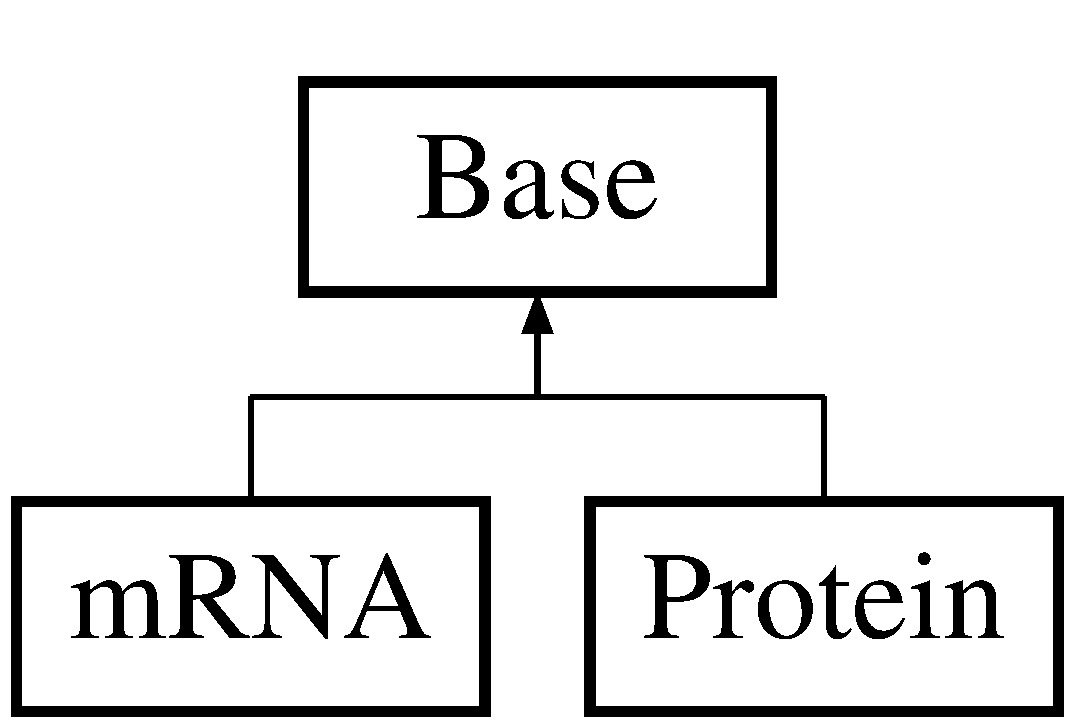
\includegraphics[height=2.000000cm]{class_base}
\end{center}
\end{figure}
\subsection*{Public Member Functions}
\begin{DoxyCompactItemize}
\item 
\hypertarget{class_base_a2539be60a003bf1153a87444870cfc50}{virtual void {\bfseries Compute} (int)=0}\label{class_base_a2539be60a003bf1153a87444870cfc50}

\end{DoxyCompactItemize}
\subsection*{Protected Attributes}
\begin{DoxyCompactItemize}
\item 
\hypertarget{class_base_af46b05bd03228ba15d40a05c15abffa0}{int {\bfseries id}}\label{class_base_af46b05bd03228ba15d40a05c15abffa0}

\item 
\hypertarget{class_base_afc939d650ee448e4b9e9302fdd8e6dae}{int {\bfseries length}}\label{class_base_afc939d650ee448e4b9e9302fdd8e6dae}

\item 
\hypertarget{class_base_a4c2c4261e4f2d0e7ebaf93bde00d3a26}{double {\bfseries dt}}\label{class_base_a4c2c4261e4f2d0e7ebaf93bde00d3a26}

\item 
\hypertarget{class_base_a262c09f4273320c819d77ec15a895980}{double $\ast$ {\bfseries abundance}}\label{class_base_a262c09f4273320c819d77ec15a895980}

\end{DoxyCompactItemize}
\subsection*{Friends}
\begin{DoxyCompactItemize}
\item 
\hypertarget{class_base_a50c933a62458087717ab7406e4cf01bc}{double $\ast$ {\bfseries Export} (int \&)}\label{class_base_a50c933a62458087717ab7406e4cf01bc}

\item 
\hypertarget{class_base_a868cf38fedb3c52291069b74bb198bf0}{void {\bfseries Simulate} ()}\label{class_base_a868cf38fedb3c52291069b74bb198bf0}

\end{DoxyCompactItemize}


The documentation for this class was generated from the following file\-:\begin{DoxyCompactItemize}
\item 
graph.\-h\end{DoxyCompactItemize}

\hypertarget{class_d_n_a}{\section{D\-N\-A Class Reference}
\label{class_d_n_a}\index{D\-N\-A@{D\-N\-A}}
}


{\ttfamily \#include $<$graph.\-h$>$}



Collaboration diagram for D\-N\-A\-:
\subsection*{Public Member Functions}
\begin{DoxyCompactItemize}
\item 
\hyperlink{class_d_n_a_a6d92499f10d383ac656e98694cc6c5e6}{D\-N\-A} (double, double, double)
\item 
void \hyperlink{class_d_n_a_a4db79a1d4530c15f30ec82cb8a502dda}{Connect} (\hyperlink{class_protein}{Protein} $\ast$)
\end{DoxyCompactItemize}
\subsection*{Private Attributes}
\begin{DoxyCompactItemize}
\item 
\hyperlink{class_protein}{Protein} $\ast$ \hyperlink{class_d_n_a_a08dd607e26ea53375e0c6d61c0c04ba9}{repressor}
\item 
double \hyperlink{class_d_n_a_ad9f4838495b5f66e494a8adb3384b919}{m}
\item 
double \hyperlink{class_d_n_a_a30c4d522f315530f9ce72e84afd6804c}{alpha}
\item 
double \hyperlink{class_d_n_a_a0dbd4309884cc23e9cbaf6cf4dc5ba0e}{epsilon}
\end{DoxyCompactItemize}
\subsection*{Friends}
\begin{DoxyCompactItemize}
\item 
class \hyperlink{class_d_n_a_a904bf77ec17baad950eb63ea5c40c6ea}{m\-R\-N\-A}
\end{DoxyCompactItemize}


\subsection{Constructor \& Destructor Documentation}
\hypertarget{class_d_n_a_a6d92499f10d383ac656e98694cc6c5e6}{\index{D\-N\-A@{D\-N\-A}!D\-N\-A@{D\-N\-A}}
\index{D\-N\-A@{D\-N\-A}!DNA@{D\-N\-A}}
\subsubsection[{D\-N\-A}]{\setlength{\rightskip}{0pt plus 5cm}D\-N\-A\-::\-D\-N\-A (
\begin{DoxyParamCaption}
\item[{double}]{mm, }
\item[{double}]{a, }
\item[{double}]{e}
\end{DoxyParamCaption}
)}}\label{class_d_n_a_a6d92499f10d383ac656e98694cc6c5e6}


\subsection{Member Function Documentation}
\hypertarget{class_d_n_a_a4db79a1d4530c15f30ec82cb8a502dda}{\index{D\-N\-A@{D\-N\-A}!Connect@{Connect}}
\index{Connect@{Connect}!DNA@{D\-N\-A}}
\subsubsection[{Connect}]{\setlength{\rightskip}{0pt plus 5cm}void D\-N\-A\-::\-Connect (
\begin{DoxyParamCaption}
\item[{{\bf Protein} $\ast$}]{p}
\end{DoxyParamCaption}
)}}\label{class_d_n_a_a4db79a1d4530c15f30ec82cb8a502dda}


\subsection{Friends And Related Function Documentation}
\hypertarget{class_d_n_a_a904bf77ec17baad950eb63ea5c40c6ea}{\index{D\-N\-A@{D\-N\-A}!m\-R\-N\-A@{m\-R\-N\-A}}
\index{m\-R\-N\-A@{m\-R\-N\-A}!DNA@{D\-N\-A}}
\subsubsection[{m\-R\-N\-A}]{\setlength{\rightskip}{0pt plus 5cm}friend class {\bf m\-R\-N\-A}\hspace{0.3cm}{\ttfamily [friend]}}}\label{class_d_n_a_a904bf77ec17baad950eb63ea5c40c6ea}


\subsection{Member Data Documentation}
\hypertarget{class_d_n_a_a30c4d522f315530f9ce72e84afd6804c}{\index{D\-N\-A@{D\-N\-A}!alpha@{alpha}}
\index{alpha@{alpha}!DNA@{D\-N\-A}}
\subsubsection[{alpha}]{\setlength{\rightskip}{0pt plus 5cm}double D\-N\-A\-::alpha\hspace{0.3cm}{\ttfamily [private]}}}\label{class_d_n_a_a30c4d522f315530f9ce72e84afd6804c}
\hypertarget{class_d_n_a_a0dbd4309884cc23e9cbaf6cf4dc5ba0e}{\index{D\-N\-A@{D\-N\-A}!epsilon@{epsilon}}
\index{epsilon@{epsilon}!DNA@{D\-N\-A}}
\subsubsection[{epsilon}]{\setlength{\rightskip}{0pt plus 5cm}double D\-N\-A\-::epsilon\hspace{0.3cm}{\ttfamily [private]}}}\label{class_d_n_a_a0dbd4309884cc23e9cbaf6cf4dc5ba0e}
\hypertarget{class_d_n_a_ad9f4838495b5f66e494a8adb3384b919}{\index{D\-N\-A@{D\-N\-A}!m@{m}}
\index{m@{m}!DNA@{D\-N\-A}}
\subsubsection[{m}]{\setlength{\rightskip}{0pt plus 5cm}double D\-N\-A\-::m\hspace{0.3cm}{\ttfamily [private]}}}\label{class_d_n_a_ad9f4838495b5f66e494a8adb3384b919}
\hypertarget{class_d_n_a_a08dd607e26ea53375e0c6d61c0c04ba9}{\index{D\-N\-A@{D\-N\-A}!repressor@{repressor}}
\index{repressor@{repressor}!DNA@{D\-N\-A}}
\subsubsection[{repressor}]{\setlength{\rightskip}{0pt plus 5cm}{\bf Protein}$\ast$ D\-N\-A\-::repressor\hspace{0.3cm}{\ttfamily [private]}}}\label{class_d_n_a_a08dd607e26ea53375e0c6d61c0c04ba9}


The documentation for this class was generated from the following file\-:\begin{DoxyCompactItemize}
\item 
\hyperlink{graph_8h}{graph.\-h}\end{DoxyCompactItemize}

\hypertarget{classweb_1_1_simulate___class_1_1_d_n_a___simulate}{\section{web.\-Simulate\-\_\-\-Class.\-D\-N\-A\-\_\-\-Simulate Class Reference}
\label{classweb_1_1_simulate___class_1_1_d_n_a___simulate}\index{web.\-Simulate\-\_\-\-Class.\-D\-N\-A\-\_\-\-Simulate@{web.\-Simulate\-\_\-\-Class.\-D\-N\-A\-\_\-\-Simulate}}
}


\subsubsection*{calculating \hyperlink{class_d_n_a}{D\-N\-A} simulation result } 


\subsection*{Public Member Functions}
\begin{DoxyCompactItemize}
\item 
def \hyperlink{classweb_1_1_simulate___class_1_1_d_n_a___simulate_a06ff5bd8c89a820405d937a5f8a837f3}{Set\-Data}
\begin{DoxyCompactList}\small\item\em Set data in class. \end{DoxyCompactList}\item 
def \hyperlink{classweb_1_1_simulate___class_1_1_d_n_a___simulate_ad17aed6fe820df86a76eae9e307c6fbc}{Set\-Activator}
\begin{DoxyCompactList}\small\item\em set activator in class \end{DoxyCompactList}\item 
def \hyperlink{classweb_1_1_simulate___class_1_1_d_n_a___simulate_af3ad470a356961ff4019e740f813e321}{Set\-Repressor}
\begin{DoxyCompactList}\small\item\em set repressor in class \end{DoxyCompactList}\item 
def \hyperlink{classweb_1_1_simulate___class_1_1_d_n_a___simulate_a467aabf0e04b68c0b813931ffdfbd86c}{Set\-Corepressor}
\begin{DoxyCompactList}\small\item\em set corepressor in class \end{DoxyCompactList}\item 
def \hyperlink{classweb_1_1_simulate___class_1_1_d_n_a___simulate_ad7ed3917ea1662b7d8ebded6ae6c9275}{Set\-Inducer}
\begin{DoxyCompactList}\small\item\em set inducer in class \end{DoxyCompactList}\end{DoxyCompactItemize}
\subsection*{Public Attributes}
\begin{DoxyCompactItemize}
\item 
\hypertarget{classweb_1_1_simulate___class_1_1_d_n_a___simulate_aa234468d2d8f7d04de55e93cb1ab0680}{{\bfseries Type}}\label{classweb_1_1_simulate___class_1_1_d_n_a___simulate_aa234468d2d8f7d04de55e93cb1ab0680}

\end{DoxyCompactItemize}
\subsection*{Static Public Attributes}
\begin{DoxyCompactItemize}
\item 
\hypertarget{classweb_1_1_simulate___class_1_1_d_n_a___simulate_a85da64f8805311e83467d99e2b4553a1}{string {\bfseries Type} = \char`\"{}\char`\"{}}\label{classweb_1_1_simulate___class_1_1_d_n_a___simulate_a85da64f8805311e83467d99e2b4553a1}

\item 
\hypertarget{classweb_1_1_simulate___class_1_1_d_n_a___simulate_a399330e85a7f32291f717b9eb846d080}{{\bfseries Copy\-Number} = None}\label{classweb_1_1_simulate___class_1_1_d_n_a___simulate_a399330e85a7f32291f717b9eb846d080}

\item 
\hypertarget{classweb_1_1_simulate___class_1_1_d_n_a___simulate_aea102d7a236466b4204e777bcbcfb1af}{{\bfseries T\-S\-Promoter} = None}\label{classweb_1_1_simulate___class_1_1_d_n_a___simulate_aea102d7a236466b4204e777bcbcfb1af}

\item 
\hypertarget{classweb_1_1_simulate___class_1_1_d_n_a___simulate_abc27d2561f40165607efd2b894fc18ef}{{\bfseries Leakage\-Rate} = None}\label{classweb_1_1_simulate___class_1_1_d_n_a___simulate_abc27d2561f40165607efd2b894fc18ef}

\item 
\hypertarget{classweb_1_1_simulate___class_1_1_d_n_a___simulate_af4973b509128336acfee906693d6af4b}{{\bfseries Ter\-E} = None}\label{classweb_1_1_simulate___class_1_1_d_n_a___simulate_af4973b509128336acfee906693d6af4b}

\item 
\hypertarget{classweb_1_1_simulate___class_1_1_d_n_a___simulate_ae298041c1b536e5ab369dff6cd3bac76}{{\bfseries Activator} = None}\label{classweb_1_1_simulate___class_1_1_d_n_a___simulate_ae298041c1b536e5ab369dff6cd3bac76}

\item 
\hypertarget{classweb_1_1_simulate___class_1_1_d_n_a___simulate_a6fc6961ca56a8c2f63f6289001092aa8}{{\bfseries Repressor} = None}\label{classweb_1_1_simulate___class_1_1_d_n_a___simulate_a6fc6961ca56a8c2f63f6289001092aa8}

\item 
\hypertarget{classweb_1_1_simulate___class_1_1_d_n_a___simulate_afe473f23d1ec1f5e576297bfa99b8d55}{{\bfseries Hill\-Coeff} = None}\label{classweb_1_1_simulate___class_1_1_d_n_a___simulate_afe473f23d1ec1f5e576297bfa99b8d55}

\item 
\hypertarget{classweb_1_1_simulate___class_1_1_d_n_a___simulate_ab41cef07d4729f53b81042b06b637fdf}{{\bfseries K} = None}\label{classweb_1_1_simulate___class_1_1_d_n_a___simulate_ab41cef07d4729f53b81042b06b637fdf}

\item 
\hypertarget{classweb_1_1_simulate___class_1_1_d_n_a___simulate_a4c01a78dc773cffe777a928a3ad8abcf}{{\bfseries Corep\-Const} = None}\label{classweb_1_1_simulate___class_1_1_d_n_a___simulate_a4c01a78dc773cffe777a928a3ad8abcf}

\item 
\hypertarget{classweb_1_1_simulate___class_1_1_d_n_a___simulate_a555c52a90c570dda2ccd7a0ec7eb00e2}{{\bfseries Ind\-Const} = None}\label{classweb_1_1_simulate___class_1_1_d_n_a___simulate_a555c52a90c570dda2ccd7a0ec7eb00e2}

\end{DoxyCompactItemize}


\subsection{Detailed Description}
\subsubsection*{calculating \hyperlink{class_d_n_a}{D\-N\-A} simulation result }

\subsection{Member Function Documentation}
\hypertarget{classweb_1_1_simulate___class_1_1_d_n_a___simulate_ad17aed6fe820df86a76eae9e307c6fbc}{\index{web\-::\-Simulate\-\_\-\-Class\-::\-D\-N\-A\-\_\-\-Simulate@{web\-::\-Simulate\-\_\-\-Class\-::\-D\-N\-A\-\_\-\-Simulate}!Set\-Activator@{Set\-Activator}}
\index{Set\-Activator@{Set\-Activator}!web::Simulate_Class::DNA_Simulate@{web\-::\-Simulate\-\_\-\-Class\-::\-D\-N\-A\-\_\-\-Simulate}}
\subsubsection[{Set\-Activator}]{\setlength{\rightskip}{0pt plus 5cm}def web.\-Simulate\-\_\-\-Class.\-D\-N\-A\-\_\-\-Simulate.\-Set\-Activator (
\begin{DoxyParamCaption}
\item[{}]{self, }
\item[{}]{activator, }
\item[{}]{k, }
\item[{}]{hillcoeff}
\end{DoxyParamCaption}
)}}\label{classweb_1_1_simulate___class_1_1_d_n_a___simulate_ad17aed6fe820df86a76eae9e307c6fbc}


set activator in class 


\begin{DoxyParams}{Parameters}
{\em activator} & name of activator \\
\hline
{\em k} & K value of activator \\
\hline
{\em hillcoeff} & hill coefficiency of activator\\
\hline
\end{DoxyParams}
\begin{DoxyReturn}{Returns}
return nothing 

 
\end{DoxyReturn}
\hypertarget{classweb_1_1_simulate___class_1_1_d_n_a___simulate_a467aabf0e04b68c0b813931ffdfbd86c}{\index{web\-::\-Simulate\-\_\-\-Class\-::\-D\-N\-A\-\_\-\-Simulate@{web\-::\-Simulate\-\_\-\-Class\-::\-D\-N\-A\-\_\-\-Simulate}!Set\-Corepressor@{Set\-Corepressor}}
\index{Set\-Corepressor@{Set\-Corepressor}!web::Simulate_Class::DNA_Simulate@{web\-::\-Simulate\-\_\-\-Class\-::\-D\-N\-A\-\_\-\-Simulate}}
\subsubsection[{Set\-Corepressor}]{\setlength{\rightskip}{0pt plus 5cm}def web.\-Simulate\-\_\-\-Class.\-D\-N\-A\-\_\-\-Simulate.\-Set\-Corepressor (
\begin{DoxyParamCaption}
\item[{}]{self, }
\item[{}]{corepressor, }
\item[{}]{k, }
\item[{}]{hillcoeff}
\end{DoxyParamCaption}
)}}\label{classweb_1_1_simulate___class_1_1_d_n_a___simulate_a467aabf0e04b68c0b813931ffdfbd86c}


set corepressor in class 


\begin{DoxyParams}{Parameters}
{\em corepressor} & name of corepressor \\
\hline
{\em k} & K value of corepressor \\
\hline
{\em hillcoeff} & hill coefficiency of corepressor\\
\hline
\end{DoxyParams}
\begin{DoxyReturn}{Returns}
return nothing 

 
\end{DoxyReturn}
\hypertarget{classweb_1_1_simulate___class_1_1_d_n_a___simulate_a06ff5bd8c89a820405d937a5f8a837f3}{\index{web\-::\-Simulate\-\_\-\-Class\-::\-D\-N\-A\-\_\-\-Simulate@{web\-::\-Simulate\-\_\-\-Class\-::\-D\-N\-A\-\_\-\-Simulate}!Set\-Data@{Set\-Data}}
\index{Set\-Data@{Set\-Data}!web::Simulate_Class::DNA_Simulate@{web\-::\-Simulate\-\_\-\-Class\-::\-D\-N\-A\-\_\-\-Simulate}}
\subsubsection[{Set\-Data}]{\setlength{\rightskip}{0pt plus 5cm}def web.\-Simulate\-\_\-\-Class.\-D\-N\-A\-\_\-\-Simulate.\-Set\-Data (
\begin{DoxyParamCaption}
\item[{}]{self, }
\item[{}]{ty, }
\item[{}]{copynumber, }
\item[{}]{tspromoter, }
\item[{}]{leakagerate, }
\item[{}]{tere}
\end{DoxyParamCaption}
)}}\label{classweb_1_1_simulate___class_1_1_d_n_a___simulate_a06ff5bd8c89a820405d937a5f8a837f3}


Set data in class. 


\begin{DoxyParams}{Parameters}
{\em ty} & type of data(constitutive, positive or negative) \\
\hline
{\em copynumber} & copy number of corresponding plasmid of component \\
\hline
{\em tspromoter} & T\-S\-Promoter of corresponding group of component \\
\hline
{\em leakagerate} & Leakage Rate of corresponding group of component \\
\hline
{\em tere} & terminator efficiency of corresponding group of component\\
\hline
\end{DoxyParams}
\begin{DoxyReturn}{Returns}
return nothing 

 
\end{DoxyReturn}
\hypertarget{classweb_1_1_simulate___class_1_1_d_n_a___simulate_ad7ed3917ea1662b7d8ebded6ae6c9275}{\index{web\-::\-Simulate\-\_\-\-Class\-::\-D\-N\-A\-\_\-\-Simulate@{web\-::\-Simulate\-\_\-\-Class\-::\-D\-N\-A\-\_\-\-Simulate}!Set\-Inducer@{Set\-Inducer}}
\index{Set\-Inducer@{Set\-Inducer}!web::Simulate_Class::DNA_Simulate@{web\-::\-Simulate\-\_\-\-Class\-::\-D\-N\-A\-\_\-\-Simulate}}
\subsubsection[{Set\-Inducer}]{\setlength{\rightskip}{0pt plus 5cm}def web.\-Simulate\-\_\-\-Class.\-D\-N\-A\-\_\-\-Simulate.\-Set\-Inducer (
\begin{DoxyParamCaption}
\item[{}]{self, }
\item[{}]{inducer, }
\item[{}]{k, }
\item[{}]{hillcoeff}
\end{DoxyParamCaption}
)}}\label{classweb_1_1_simulate___class_1_1_d_n_a___simulate_ad7ed3917ea1662b7d8ebded6ae6c9275}


set inducer in class 


\begin{DoxyParams}{Parameters}
{\em inducer} & name of inducer \\
\hline
{\em k} & K value of inducer \\
\hline
{\em hillcoeff} & hill coefficiency of inducer\\
\hline
\end{DoxyParams}
\begin{DoxyReturn}{Returns}
return nothing 

 
\end{DoxyReturn}
\hypertarget{classweb_1_1_simulate___class_1_1_d_n_a___simulate_af3ad470a356961ff4019e740f813e321}{\index{web\-::\-Simulate\-\_\-\-Class\-::\-D\-N\-A\-\_\-\-Simulate@{web\-::\-Simulate\-\_\-\-Class\-::\-D\-N\-A\-\_\-\-Simulate}!Set\-Repressor@{Set\-Repressor}}
\index{Set\-Repressor@{Set\-Repressor}!web::Simulate_Class::DNA_Simulate@{web\-::\-Simulate\-\_\-\-Class\-::\-D\-N\-A\-\_\-\-Simulate}}
\subsubsection[{Set\-Repressor}]{\setlength{\rightskip}{0pt plus 5cm}def web.\-Simulate\-\_\-\-Class.\-D\-N\-A\-\_\-\-Simulate.\-Set\-Repressor (
\begin{DoxyParamCaption}
\item[{}]{self, }
\item[{}]{repressor, }
\item[{}]{k, }
\item[{}]{hillcoeff}
\end{DoxyParamCaption}
)}}\label{classweb_1_1_simulate___class_1_1_d_n_a___simulate_af3ad470a356961ff4019e740f813e321}


set repressor in class 


\begin{DoxyParams}{Parameters}
{\em repressor} & name of repressor \\
\hline
{\em k} & K value of repressor \\
\hline
{\em hillcoeff} & hill coefficiency of repressor\\
\hline
\end{DoxyParams}
\begin{DoxyReturn}{Returns}
return nothing 

 
\end{DoxyReturn}


The documentation for this class was generated from the following file\-:\begin{DoxyCompactItemize}
\item 
\hyperlink{_simulate___class_8py}{Simulate\-\_\-\-Class.\-py}\end{DoxyCompactItemize}

\hypertarget{classweb_1_1encrypt_1_1_encrypt}{\section{web.\-encrypt.\-Encrypt Class Reference}
\label{classweb_1_1encrypt_1_1_encrypt}\index{web.\-encrypt.\-Encrypt@{web.\-encrypt.\-Encrypt}}
}


\subsubsection*{the class that can provide R\-S\-A method } 


\subsection*{Public Member Functions}
\begin{DoxyCompactItemize}
\item 
def \hyperlink{classweb_1_1encrypt_1_1_encrypt_a7ac013ef450d16011e76b7af95c25f3d}{\-\_\-\-\_\-init\-\_\-\-\_\-}
\item 
def \hyperlink{classweb_1_1encrypt_1_1_encrypt_ad9c50ce7eec9117081e4d86a9bfd87c9}{get\-Public\-Key}
\begin{DoxyCompactList}\small\item\em get the public key \end{DoxyCompactList}\item 
def \hyperlink{classweb_1_1encrypt_1_1_encrypt_afcab4d2eea9fe8213086a46253e72316}{decrypt}
\begin{DoxyCompactList}\small\item\em decrypt a string \end{DoxyCompactList}\end{DoxyCompactItemize}
\subsection*{Public Attributes}
\begin{DoxyCompactItemize}
\item 
\hyperlink{classweb_1_1encrypt_1_1_encrypt_a1e54531b2aac210260199608edc7f62c}{public\-Key}
\item 
\hyperlink{classweb_1_1encrypt_1_1_encrypt_a1145a5b40bf2a2ff38383b34d4d86dc8}{private\-Key}
\end{DoxyCompactItemize}


\subsection{Detailed Description}
\subsubsection*{the class that can provide R\-S\-A method }

\subsection{Constructor \& Destructor Documentation}
\hypertarget{classweb_1_1encrypt_1_1_encrypt_a7ac013ef450d16011e76b7af95c25f3d}{\index{web\-::encrypt\-::\-Encrypt@{web\-::encrypt\-::\-Encrypt}!\-\_\-\-\_\-init\-\_\-\-\_\-@{\-\_\-\-\_\-init\-\_\-\-\_\-}}
\index{\-\_\-\-\_\-init\-\_\-\-\_\-@{\-\_\-\-\_\-init\-\_\-\-\_\-}!web::encrypt::Encrypt@{web\-::encrypt\-::\-Encrypt}}
\subsubsection[{\-\_\-\-\_\-init\-\_\-\-\_\-}]{\setlength{\rightskip}{0pt plus 5cm}def web.\-encrypt.\-Encrypt.\-\_\-\-\_\-init\-\_\-\-\_\- (
\begin{DoxyParamCaption}
\item[{}]{self}
\end{DoxyParamCaption}
)}}\label{classweb_1_1encrypt_1_1_encrypt_a7ac013ef450d16011e76b7af95c25f3d}


\subsection{Member Function Documentation}
\hypertarget{classweb_1_1encrypt_1_1_encrypt_afcab4d2eea9fe8213086a46253e72316}{\index{web\-::encrypt\-::\-Encrypt@{web\-::encrypt\-::\-Encrypt}!decrypt@{decrypt}}
\index{decrypt@{decrypt}!web::encrypt::Encrypt@{web\-::encrypt\-::\-Encrypt}}
\subsubsection[{decrypt}]{\setlength{\rightskip}{0pt plus 5cm}def web.\-encrypt.\-Encrypt.\-decrypt (
\begin{DoxyParamCaption}
\item[{}]{self, }
\item[{}]{crypto}
\end{DoxyParamCaption}
)}}\label{classweb_1_1encrypt_1_1_encrypt_afcab4d2eea9fe8213086a46253e72316}


decrypt a string 


\begin{DoxyParams}{Parameters}
{\em self} & \\
\hline
{\em crypto} & the crypto string\\
\hline
\end{DoxyParams}
\begin{DoxyReturn}{Returns}
return the original string using the private\-Key 

 
\end{DoxyReturn}
\hypertarget{classweb_1_1encrypt_1_1_encrypt_ad9c50ce7eec9117081e4d86a9bfd87c9}{\index{web\-::encrypt\-::\-Encrypt@{web\-::encrypt\-::\-Encrypt}!get\-Public\-Key@{get\-Public\-Key}}
\index{get\-Public\-Key@{get\-Public\-Key}!web::encrypt::Encrypt@{web\-::encrypt\-::\-Encrypt}}
\subsubsection[{get\-Public\-Key}]{\setlength{\rightskip}{0pt plus 5cm}def web.\-encrypt.\-Encrypt.\-get\-Public\-Key (
\begin{DoxyParamCaption}
\item[{}]{self}
\end{DoxyParamCaption}
)}}\label{classweb_1_1encrypt_1_1_encrypt_ad9c50ce7eec9117081e4d86a9bfd87c9}


get the public key 


\begin{DoxyParams}{Parameters}
{\em self} & \\
\hline
\end{DoxyParams}
\begin{DoxyReturn}{Returns}
return the public key 

 
\end{DoxyReturn}


\subsection{Member Data Documentation}
\hypertarget{classweb_1_1encrypt_1_1_encrypt_a1145a5b40bf2a2ff38383b34d4d86dc8}{\index{web\-::encrypt\-::\-Encrypt@{web\-::encrypt\-::\-Encrypt}!private\-Key@{private\-Key}}
\index{private\-Key@{private\-Key}!web::encrypt::Encrypt@{web\-::encrypt\-::\-Encrypt}}
\subsubsection[{private\-Key}]{\setlength{\rightskip}{0pt plus 5cm}web.\-encrypt.\-Encrypt.\-private\-Key}}\label{classweb_1_1encrypt_1_1_encrypt_a1145a5b40bf2a2ff38383b34d4d86dc8}
\hypertarget{classweb_1_1encrypt_1_1_encrypt_a1e54531b2aac210260199608edc7f62c}{\index{web\-::encrypt\-::\-Encrypt@{web\-::encrypt\-::\-Encrypt}!public\-Key@{public\-Key}}
\index{public\-Key@{public\-Key}!web::encrypt::Encrypt@{web\-::encrypt\-::\-Encrypt}}
\subsubsection[{public\-Key}]{\setlength{\rightskip}{0pt plus 5cm}web.\-encrypt.\-Encrypt.\-public\-Key}}\label{classweb_1_1encrypt_1_1_encrypt_a1e54531b2aac210260199608edc7f62c}


The documentation for this class was generated from the following file\-:\begin{DoxyCompactItemize}
\item 
\hyperlink{encrypt_8py}{encrypt.\-py}\end{DoxyCompactItemize}

\hypertarget{classweb_1_1_simulate___class_1_1_illegal_setting}{\section{web.\-Simulate\-\_\-\-Class.\-Illegal\-Setting Class Reference}
\label{classweb_1_1_simulate___class_1_1_illegal_setting}\index{web.\-Simulate\-\_\-\-Class.\-Illegal\-Setting@{web.\-Simulate\-\_\-\-Class.\-Illegal\-Setting}}
}
Inheritance diagram for web.\-Simulate\-\_\-\-Class.\-Illegal\-Setting\-:\begin{figure}[H]
\begin{center}
\leavevmode
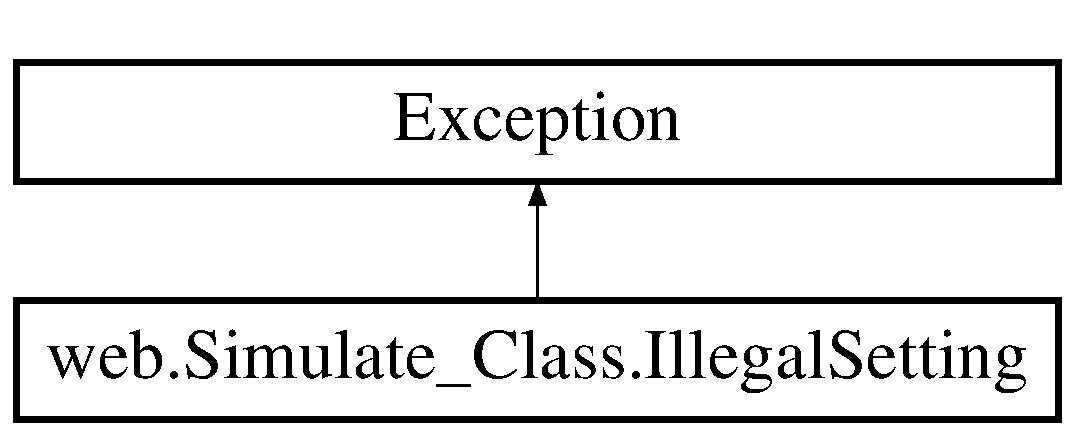
\includegraphics[height=2.000000cm]{classweb_1_1_simulate___class_1_1_illegal_setting}
\end{center}
\end{figure}


The documentation for this class was generated from the following file\-:\begin{DoxyCompactItemize}
\item 
\hyperlink{_simulate___class_8py}{Simulate\-\_\-\-Class.\-py}\end{DoxyCompactItemize}

\hypertarget{classweb_1_1_simulate___class_1_1_invalid_parameter}{\section{web.\-Simulate\-\_\-\-Class.\-Invalid\-Parameter Class Reference}
\label{classweb_1_1_simulate___class_1_1_invalid_parameter}\index{web.\-Simulate\-\_\-\-Class.\-Invalid\-Parameter@{web.\-Simulate\-\_\-\-Class.\-Invalid\-Parameter}}
}
Inheritance diagram for web.\-Simulate\-\_\-\-Class.\-Invalid\-Parameter\-:\begin{figure}[H]
\begin{center}
\leavevmode
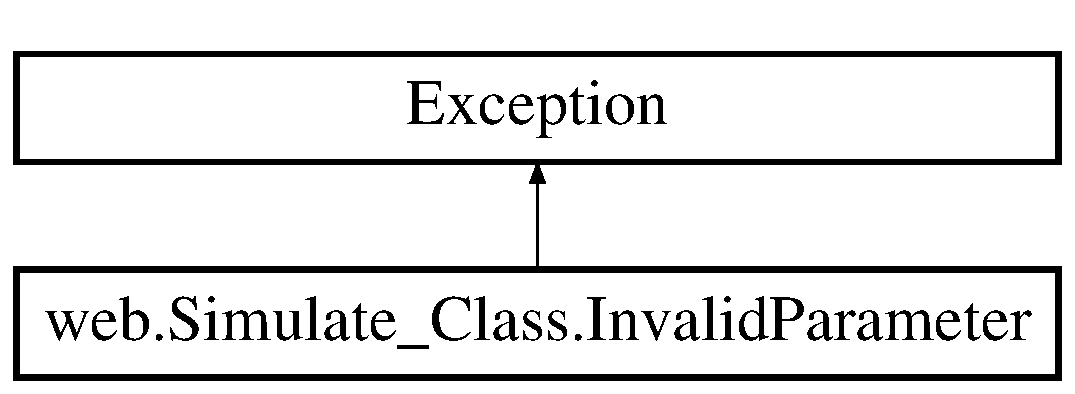
\includegraphics[height=2.000000cm]{classweb_1_1_simulate___class_1_1_invalid_parameter}
\end{center}
\end{figure}


The documentation for this class was generated from the following file\-:\begin{DoxyCompactItemize}
\item 
\hyperlink{_simulate___class_8py}{Simulate\-\_\-\-Class.\-py}\end{DoxyCompactItemize}

\hypertarget{classweb_1_1modeling_1_1modeling}{\section{web.\-modeling.\-modeling Class Reference}
\label{classweb_1_1modeling_1_1modeling}\index{web.\-modeling.\-modeling@{web.\-modeling.\-modeling}}
}
\subsection*{Public Member Functions}
\begin{DoxyCompactItemize}
\item 
\hypertarget{classweb_1_1modeling_1_1modeling_a7898b83d4325000468bf3b19dd0cf009}{def {\bfseries \-\_\-\-\_\-init\-\_\-\-\_\-}}\label{classweb_1_1modeling_1_1modeling_a7898b83d4325000468bf3b19dd0cf009}

\item 
\hypertarget{classweb_1_1modeling_1_1modeling_ad21a9030cd229dc73b6318abff8733e6}{def {\bfseries depressing\-Function}}\label{classweb_1_1modeling_1_1modeling_ad21a9030cd229dc73b6318abff8733e6}

\end{DoxyCompactItemize}
\subsection*{Public Attributes}
\begin{DoxyCompactItemize}
\item 
\hypertarget{classweb_1_1modeling_1_1modeling_affbc9a007f7b35ef14afce145c58bf18}{{\bfseries db}}\label{classweb_1_1modeling_1_1modeling_affbc9a007f7b35ef14afce145c58bf18}

\item 
\hypertarget{classweb_1_1modeling_1_1modeling_a7305302d2cd99859e0641132ac9ac0f3}{{\bfseries A\-Expression\-Value\-Record}}\label{classweb_1_1modeling_1_1modeling_a7305302d2cd99859e0641132ac9ac0f3}

\item 
\hypertarget{classweb_1_1modeling_1_1modeling_a8fb8abde81146a93ee8f7e0ec8fedf7f}{{\bfseries A\-Promoter}}\label{classweb_1_1modeling_1_1modeling_a8fb8abde81146a93ee8f7e0ec8fedf7f}

\item 
\hypertarget{classweb_1_1modeling_1_1modeling_ad8689aeec5372b03c7455f53d32cc1d8}{{\bfseries A\-Plasmid\-Backbone}}\label{classweb_1_1modeling_1_1modeling_ad8689aeec5372b03c7455f53d32cc1d8}

\item 
\hypertarget{classweb_1_1modeling_1_1modeling_ab2ab0f6fc77ef28f58988fffed95fa74}{{\bfseries B\-Expression\-Value\-Record}}\label{classweb_1_1modeling_1_1modeling_ab2ab0f6fc77ef28f58988fffed95fa74}

\item 
\hypertarget{classweb_1_1modeling_1_1modeling_a96fa7c50494910911cd1bb5e0fd6c247}{{\bfseries B\-Promoter}}\label{classweb_1_1modeling_1_1modeling_a96fa7c50494910911cd1bb5e0fd6c247}

\item 
\hypertarget{classweb_1_1modeling_1_1modeling_a18419f401d8b614ce048cd4f61fe3720}{{\bfseries B\-Plasmid\-Backbone}}\label{classweb_1_1modeling_1_1modeling_a18419f401d8b614ce048cd4f61fe3720}

\item 
\hypertarget{classweb_1_1modeling_1_1modeling_a6da71e7f269b891b00412fc6897c9747}{{\bfseries Protein\-A}}\label{classweb_1_1modeling_1_1modeling_a6da71e7f269b891b00412fc6897c9747}

\item 
\hypertarget{classweb_1_1modeling_1_1modeling_aff3389950cb599a298b6370a2dad0185}{{\bfseries Protein\-B}}\label{classweb_1_1modeling_1_1modeling_aff3389950cb599a298b6370a2dad0185}

\item 
\hypertarget{classweb_1_1modeling_1_1modeling_a4cc11ff2adba839163240e9ea66ef398}{{\bfseries R\-B\-S}}\label{classweb_1_1modeling_1_1modeling_a4cc11ff2adba839163240e9ea66ef398}

\item 
\hypertarget{classweb_1_1modeling_1_1modeling_a0314c62c089feb8e1d85448cc94f7900}{{\bfseries Repressor\-Table}}\label{classweb_1_1modeling_1_1modeling_a0314c62c089feb8e1d85448cc94f7900}

\end{DoxyCompactItemize}


The documentation for this class was generated from the following file\-:\begin{DoxyCompactItemize}
\item 
modeling.\-py\end{DoxyCompactItemize}

\hypertarget{classm_r_n_a}{\section{m\-R\-N\-A Class Reference}
\label{classm_r_n_a}\index{m\-R\-N\-A@{m\-R\-N\-A}}
}


{\ttfamily \#include $<$graph.\-h$>$}

Inheritance diagram for m\-R\-N\-A\-:\begin{figure}[H]
\begin{center}
\leavevmode
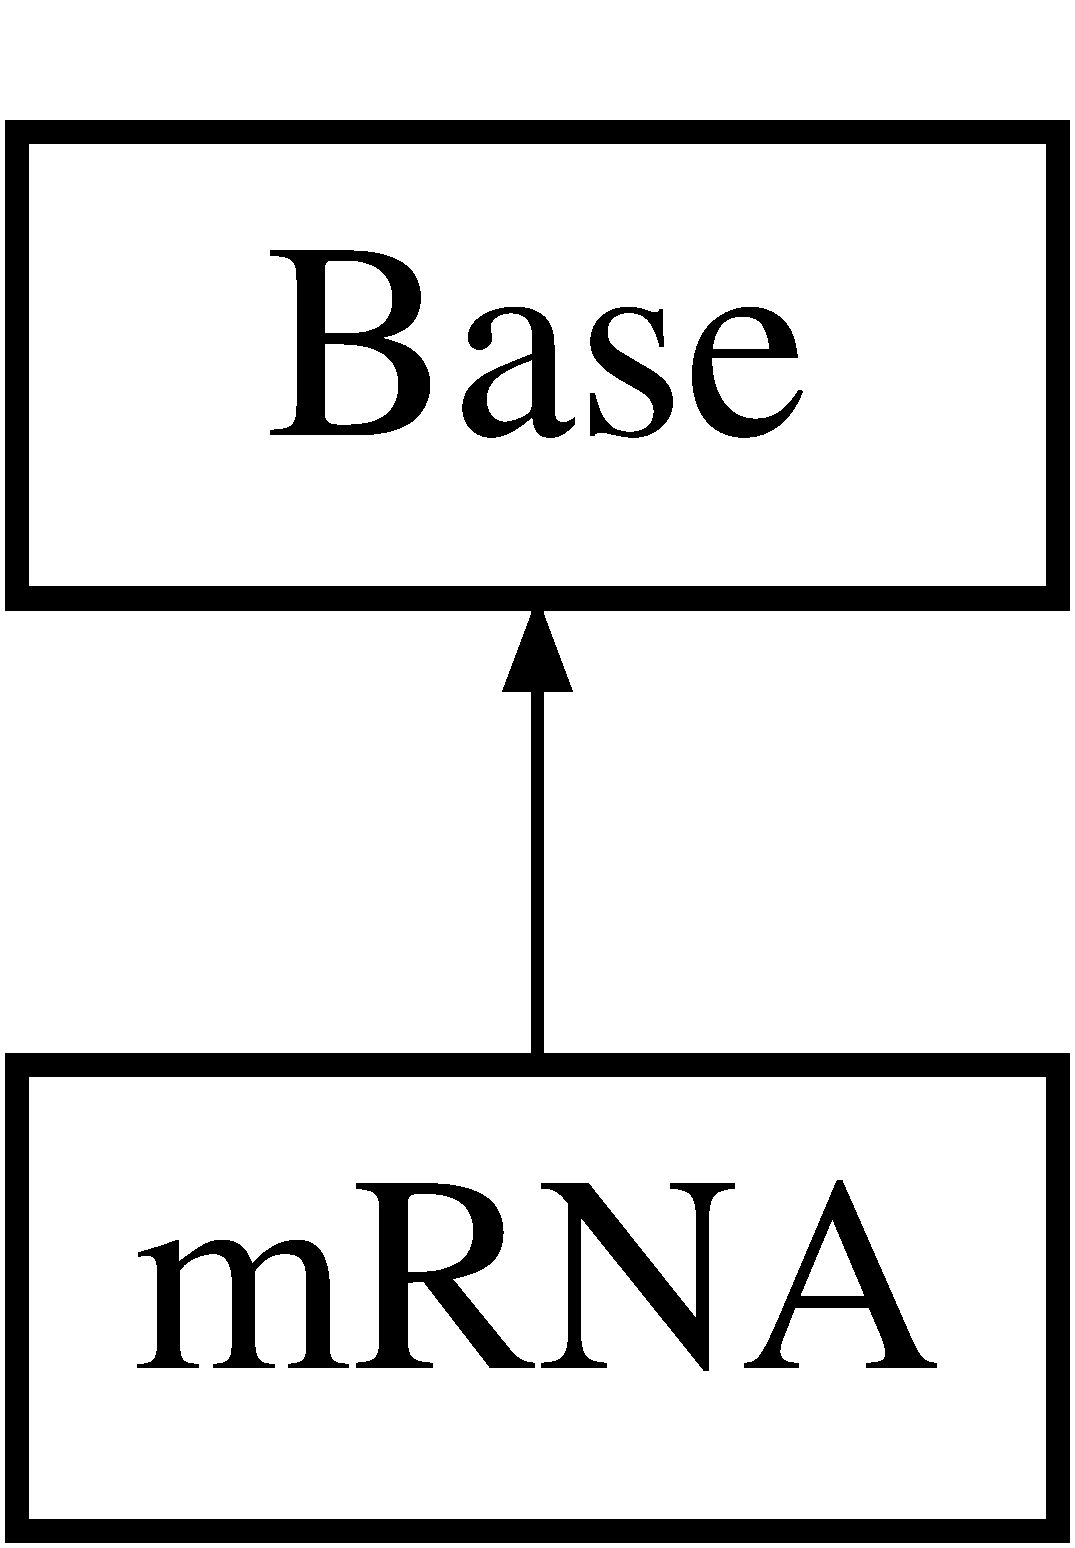
\includegraphics[height=2.000000cm]{classm_r_n_a}
\end{center}
\end{figure}
\subsection*{Public Member Functions}
\begin{DoxyCompactItemize}
\item 
\hyperlink{classm_r_n_a_a1fc26dc1fe542e23f9d374533600b9fb}{m\-R\-N\-A} (double, double, double, double)
\item 
void \hyperlink{classm_r_n_a_ac010324e6b1dc61fb8e1391b219acb2c}{Connect} (\hyperlink{class_d_n_a}{D\-N\-A} $\ast$)
\item 
void \hyperlink{classm_r_n_a_a490f8026d612c405ce2678a4d15cf7a8}{Compute} (int)
\end{DoxyCompactItemize}
\subsection*{Private Attributes}
\begin{DoxyCompactItemize}
\item 
\hyperlink{class_d_n_a}{D\-N\-A} $\ast$ \hyperlink{classm_r_n_a_ace67bd5431ec023732e05049e5ca9a4b}{dna}
\item 
double \hyperlink{classm_r_n_a_a07cdcbe61a2af4fc74751521e0c7920e}{v\-\_\-max}
\item 
double \hyperlink{classm_r_n_a_ace3b5460f5ed647cbe52e6a86e8d6ef7}{k\-\_\-mich}
\item 
double \hyperlink{classm_r_n_a_ac4e84c4700ca924196809e36fa17c5b7}{k\-\_\-deg}
\end{DoxyCompactItemize}
\subsection*{Friends}
\begin{DoxyCompactItemize}
\item 
class \hyperlink{classm_r_n_a_a2cc8b86817f46f61585ecf591984f8eb}{Protein}
\end{DoxyCompactItemize}
\subsection*{Additional Inherited Members}


\subsection{Constructor \& Destructor Documentation}
\hypertarget{classm_r_n_a_a1fc26dc1fe542e23f9d374533600b9fb}{\index{m\-R\-N\-A@{m\-R\-N\-A}!m\-R\-N\-A@{m\-R\-N\-A}}
\index{m\-R\-N\-A@{m\-R\-N\-A}!mRNA@{m\-R\-N\-A}}
\subsubsection[{m\-R\-N\-A}]{\setlength{\rightskip}{0pt plus 5cm}m\-R\-N\-A\-::m\-R\-N\-A (
\begin{DoxyParamCaption}
\item[{double}]{v, }
\item[{double}]{km, }
\item[{double}]{kd, }
\item[{double}]{ini}
\end{DoxyParamCaption}
)}}\label{classm_r_n_a_a1fc26dc1fe542e23f9d374533600b9fb}


\subsection{Member Function Documentation}
\hypertarget{classm_r_n_a_a490f8026d612c405ce2678a4d15cf7a8}{\index{m\-R\-N\-A@{m\-R\-N\-A}!Compute@{Compute}}
\index{Compute@{Compute}!mRNA@{m\-R\-N\-A}}
\subsubsection[{Compute}]{\setlength{\rightskip}{0pt plus 5cm}void m\-R\-N\-A\-::\-Compute (
\begin{DoxyParamCaption}
\item[{int}]{n}
\end{DoxyParamCaption}
)\hspace{0.3cm}{\ttfamily [virtual]}}}\label{classm_r_n_a_a490f8026d612c405ce2678a4d15cf7a8}


Implements \hyperlink{class_base_a2539be60a003bf1153a87444870cfc50}{Base}.

\hypertarget{classm_r_n_a_ac010324e6b1dc61fb8e1391b219acb2c}{\index{m\-R\-N\-A@{m\-R\-N\-A}!Connect@{Connect}}
\index{Connect@{Connect}!mRNA@{m\-R\-N\-A}}
\subsubsection[{Connect}]{\setlength{\rightskip}{0pt plus 5cm}void m\-R\-N\-A\-::\-Connect (
\begin{DoxyParamCaption}
\item[{{\bf D\-N\-A} $\ast$}]{d}
\end{DoxyParamCaption}
)}}\label{classm_r_n_a_ac010324e6b1dc61fb8e1391b219acb2c}


\subsection{Friends And Related Function Documentation}
\hypertarget{classm_r_n_a_a2cc8b86817f46f61585ecf591984f8eb}{\index{m\-R\-N\-A@{m\-R\-N\-A}!Protein@{Protein}}
\index{Protein@{Protein}!mRNA@{m\-R\-N\-A}}
\subsubsection[{Protein}]{\setlength{\rightskip}{0pt plus 5cm}friend class {\bf Protein}\hspace{0.3cm}{\ttfamily [friend]}}}\label{classm_r_n_a_a2cc8b86817f46f61585ecf591984f8eb}


\subsection{Member Data Documentation}
\hypertarget{classm_r_n_a_ace67bd5431ec023732e05049e5ca9a4b}{\index{m\-R\-N\-A@{m\-R\-N\-A}!dna@{dna}}
\index{dna@{dna}!mRNA@{m\-R\-N\-A}}
\subsubsection[{dna}]{\setlength{\rightskip}{0pt plus 5cm}{\bf D\-N\-A}$\ast$ m\-R\-N\-A\-::dna\hspace{0.3cm}{\ttfamily [private]}}}\label{classm_r_n_a_ace67bd5431ec023732e05049e5ca9a4b}
\hypertarget{classm_r_n_a_ac4e84c4700ca924196809e36fa17c5b7}{\index{m\-R\-N\-A@{m\-R\-N\-A}!k\-\_\-deg@{k\-\_\-deg}}
\index{k\-\_\-deg@{k\-\_\-deg}!mRNA@{m\-R\-N\-A}}
\subsubsection[{k\-\_\-deg}]{\setlength{\rightskip}{0pt plus 5cm}double m\-R\-N\-A\-::k\-\_\-deg\hspace{0.3cm}{\ttfamily [private]}}}\label{classm_r_n_a_ac4e84c4700ca924196809e36fa17c5b7}
\hypertarget{classm_r_n_a_ace3b5460f5ed647cbe52e6a86e8d6ef7}{\index{m\-R\-N\-A@{m\-R\-N\-A}!k\-\_\-mich@{k\-\_\-mich}}
\index{k\-\_\-mich@{k\-\_\-mich}!mRNA@{m\-R\-N\-A}}
\subsubsection[{k\-\_\-mich}]{\setlength{\rightskip}{0pt plus 5cm}double m\-R\-N\-A\-::k\-\_\-mich\hspace{0.3cm}{\ttfamily [private]}}}\label{classm_r_n_a_ace3b5460f5ed647cbe52e6a86e8d6ef7}
\hypertarget{classm_r_n_a_a07cdcbe61a2af4fc74751521e0c7920e}{\index{m\-R\-N\-A@{m\-R\-N\-A}!v\-\_\-max@{v\-\_\-max}}
\index{v\-\_\-max@{v\-\_\-max}!mRNA@{m\-R\-N\-A}}
\subsubsection[{v\-\_\-max}]{\setlength{\rightskip}{0pt plus 5cm}double m\-R\-N\-A\-::v\-\_\-max\hspace{0.3cm}{\ttfamily [private]}}}\label{classm_r_n_a_a07cdcbe61a2af4fc74751521e0c7920e}


The documentation for this class was generated from the following file\-:\begin{DoxyCompactItemize}
\item 
\hyperlink{graph_8h}{graph.\-h}\end{DoxyCompactItemize}

\hypertarget{classweb_1_1_simulate___class_1_1m_r_n_a___simulate}{\section{web.\-Simulate\-\_\-\-Class.\-m\-R\-N\-A\-\_\-\-Simulate Class Reference}
\label{classweb_1_1_simulate___class_1_1m_r_n_a___simulate}\index{web.\-Simulate\-\_\-\-Class.\-m\-R\-N\-A\-\_\-\-Simulate@{web.\-Simulate\-\_\-\-Class.\-m\-R\-N\-A\-\_\-\-Simulate}}
}
\subsection*{Public Member Functions}
\begin{DoxyCompactItemize}
\item 
\hypertarget{classweb_1_1_simulate___class_1_1m_r_n_a___simulate_aafa306e52e6cd8565e2abc96336bacbf}{def {\bfseries Set\-Data}}\label{classweb_1_1_simulate___class_1_1m_r_n_a___simulate_aafa306e52e6cd8565e2abc96336bacbf}

\item 
\hypertarget{classweb_1_1_simulate___class_1_1m_r_n_a___simulate_a4af7cedb8c3df5fcd581affc57e7afca}{def {\bfseries Connect}}\label{classweb_1_1_simulate___class_1_1m_r_n_a___simulate_a4af7cedb8c3df5fcd581affc57e7afca}

\item 
\hypertarget{classweb_1_1_simulate___class_1_1m_r_n_a___simulate_a8b9036fb94041c3247f18ab5b7d28216}{def {\bfseries Ini\-Concen}}\label{classweb_1_1_simulate___class_1_1m_r_n_a___simulate_a8b9036fb94041c3247f18ab5b7d28216}

\item 
\hypertarget{classweb_1_1_simulate___class_1_1m_r_n_a___simulate_ab96aa173aa7a27b60a60c3cddc05b41b}{def {\bfseries Compute\-\_\-\-Concen}}\label{classweb_1_1_simulate___class_1_1m_r_n_a___simulate_ab96aa173aa7a27b60a60c3cddc05b41b}

\end{DoxyCompactItemize}
\subsection*{Public Attributes}
\begin{DoxyCompactItemize}
\item 
\hypertarget{classweb_1_1_simulate___class_1_1m_r_n_a___simulate_a89a68a9662a7c802b3b9d7436649920f}{{\bfseries Concen}}\label{classweb_1_1_simulate___class_1_1m_r_n_a___simulate_a89a68a9662a7c802b3b9d7436649920f}

\end{DoxyCompactItemize}
\subsection*{Static Public Attributes}
\begin{DoxyCompactItemize}
\item 
\hypertarget{classweb_1_1_simulate___class_1_1m_r_n_a___simulate_aff71f631c32c2e13789fb4f2e413feb5}{{\bfseries Dt} = None}\label{classweb_1_1_simulate___class_1_1m_r_n_a___simulate_aff71f631c32c2e13789fb4f2e413feb5}

\item 
\hypertarget{classweb_1_1_simulate___class_1_1m_r_n_a___simulate_a1fbca90fe65ec4c5a6e07ef6aab4ef4f}{{\bfseries Time\-Len} = None}\label{classweb_1_1_simulate___class_1_1m_r_n_a___simulate_a1fbca90fe65ec4c5a6e07ef6aab4ef4f}

\item 
\hypertarget{classweb_1_1_simulate___class_1_1m_r_n_a___simulate_a8d08b83d4273c7c21c20fedc33d71d46}{list {\bfseries Concen} = \mbox{[}$\,$\mbox{]}}\label{classweb_1_1_simulate___class_1_1m_r_n_a___simulate_a8d08b83d4273c7c21c20fedc33d71d46}

\item 
\hypertarget{classweb_1_1_simulate___class_1_1m_r_n_a___simulate_a93f85081905b6beb3c395793f15b2956}{{\bfseries D\-N\-A} = None}\label{classweb_1_1_simulate___class_1_1m_r_n_a___simulate_a93f85081905b6beb3c395793f15b2956}

\item 
\hypertarget{classweb_1_1_simulate___class_1_1m_r_n_a___simulate_a0f1d34dcecf981a5dac457ce57260ead}{{\bfseries Transl\-E} = None}\label{classweb_1_1_simulate___class_1_1m_r_n_a___simulate_a0f1d34dcecf981a5dac457ce57260ead}

\item 
\hypertarget{classweb_1_1_simulate___class_1_1m_r_n_a___simulate_ab0f22fbf0ee72dcac2743805b982aab8}{{\bfseries Deg\-Rate} = None}\label{classweb_1_1_simulate___class_1_1m_r_n_a___simulate_ab0f22fbf0ee72dcac2743805b982aab8}

\end{DoxyCompactItemize}


The documentation for this class was generated from the following file\-:\begin{DoxyCompactItemize}
\item 
\hyperlink{_simulate___class_8py}{Simulate\-\_\-\-Class.\-py}\end{DoxyCompactItemize}

\hypertarget{class_protein}{\section{Protein Class Reference}
\label{class_protein}\index{Protein@{Protein}}
}
Inheritance diagram for Protein\-:\begin{figure}[H]
\begin{center}
\leavevmode
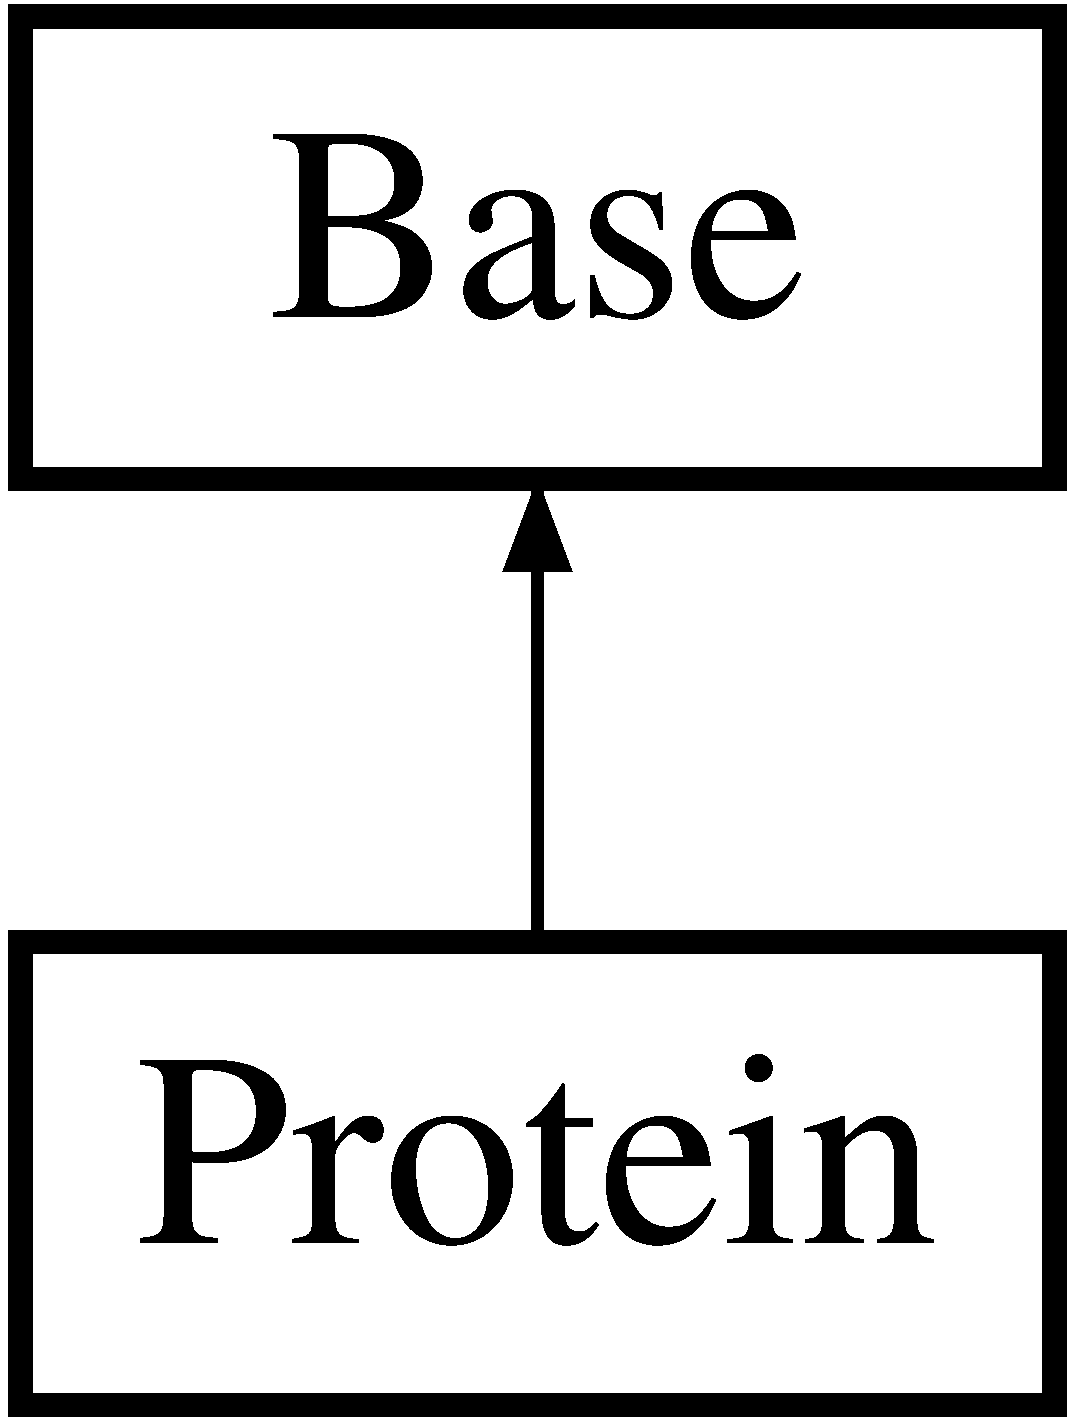
\includegraphics[height=2.000000cm]{class_protein}
\end{center}
\end{figure}
\subsection*{Public Member Functions}
\begin{DoxyCompactItemize}
\item 
\hypertarget{class_protein_a9f0a706232fd3e68c15263e2102fec02}{{\bfseries Protein} (double, double)}\label{class_protein_a9f0a706232fd3e68c15263e2102fec02}

\item 
\hypertarget{class_protein_a52cf8da9e08eeb67b44114af2d12f45c}{void {\bfseries Connect} (\hyperlink{classm_r_n_a}{m\-R\-N\-A} $\ast$)}\label{class_protein_a52cf8da9e08eeb67b44114af2d12f45c}

\item 
\hypertarget{class_protein_af977204f0e2ffe5544bcab971d5eeb0d}{void {\bfseries Compute} (int)}\label{class_protein_af977204f0e2ffe5544bcab971d5eeb0d}

\end{DoxyCompactItemize}
\subsection*{Friends}
\begin{DoxyCompactItemize}
\item 
\hypertarget{class_protein_a904bf77ec17baad950eb63ea5c40c6ea}{class {\bfseries m\-R\-N\-A}}\label{class_protein_a904bf77ec17baad950eb63ea5c40c6ea}

\end{DoxyCompactItemize}
\subsection*{Additional Inherited Members}


The documentation for this class was generated from the following file\-:\begin{DoxyCompactItemize}
\item 
graph.\-h\end{DoxyCompactItemize}

\hypertarget{classweb_1_1_simulate___class_1_1_protein___simulate}{\section{web.\-Simulate\-\_\-\-Class.\-Protein\-\_\-\-Simulate Class Reference}
\label{classweb_1_1_simulate___class_1_1_protein___simulate}\index{web.\-Simulate\-\_\-\-Class.\-Protein\-\_\-\-Simulate@{web.\-Simulate\-\_\-\-Class.\-Protein\-\_\-\-Simulate}}
}
\subsection*{Public Member Functions}
\begin{DoxyCompactItemize}
\item 
def \hyperlink{classweb_1_1_simulate___class_1_1_protein___simulate_aed90abad02aad5dc6ac31a344032b8c8}{Set\-Data}
\item 
def \hyperlink{classweb_1_1_simulate___class_1_1_protein___simulate_a25ef40b09e3b2ad608d7fd32dfbbc552}{Ini\-Concen}
\item 
def \hyperlink{classweb_1_1_simulate___class_1_1_protein___simulate_ad8e95c5ff42680746fd7f0e66dfefa95}{Connect}
\item 
def \hyperlink{classweb_1_1_simulate___class_1_1_protein___simulate_ac7de7384d587c3bc575e762ad40d8446}{Compute\-\_\-\-Concen}
\end{DoxyCompactItemize}
\subsection*{Public Attributes}
\begin{DoxyCompactItemize}
\item 
\hyperlink{classweb_1_1_simulate___class_1_1_protein___simulate_ac37e685db664715fb1f7a71d9064d80d}{Concen}
\end{DoxyCompactItemize}
\subsection*{Static Public Attributes}
\begin{DoxyCompactItemize}
\item 
\hyperlink{classweb_1_1_simulate___class_1_1_protein___simulate_a989acf6cadfdaf26684d13f36dc63adb}{Dt} = None
\item 
\hyperlink{classweb_1_1_simulate___class_1_1_protein___simulate_a50edacbd205b198ab95cdb5fc7f9635e}{Time\-Len} = None
\item 
list \hyperlink{classweb_1_1_simulate___class_1_1_protein___simulate_a446c78bb62c53d12797f4e15e634b4ac}{Concen} = \mbox{[}$\,$\mbox{]}
\item 
\hyperlink{classweb_1_1_simulate___class_1_1_protein___simulate_a7b63979d25ab27dceed5ec84fb2d1345}{m\-R\-N\-A} = None
\item 
\hyperlink{classweb_1_1_simulate___class_1_1_protein___simulate_adbb5f457e3feae482778dd6fe5ff7788}{Deg\-Rate} = None
\end{DoxyCompactItemize}


\subsection{Member Function Documentation}
\hypertarget{classweb_1_1_simulate___class_1_1_protein___simulate_ac7de7384d587c3bc575e762ad40d8446}{\index{web\-::\-Simulate\-\_\-\-Class\-::\-Protein\-\_\-\-Simulate@{web\-::\-Simulate\-\_\-\-Class\-::\-Protein\-\_\-\-Simulate}!Compute\-\_\-\-Concen@{Compute\-\_\-\-Concen}}
\index{Compute\-\_\-\-Concen@{Compute\-\_\-\-Concen}!web::Simulate_Class::Protein_Simulate@{web\-::\-Simulate\-\_\-\-Class\-::\-Protein\-\_\-\-Simulate}}
\subsubsection[{Compute\-\_\-\-Concen}]{\setlength{\rightskip}{0pt plus 5cm}def web.\-Simulate\-\_\-\-Class.\-Protein\-\_\-\-Simulate.\-Compute\-\_\-\-Concen (
\begin{DoxyParamCaption}
\item[{}]{self, }
\item[{}]{n, }
\item[{}]{is\-Stochastic}
\end{DoxyParamCaption}
)}}\label{classweb_1_1_simulate___class_1_1_protein___simulate_ac7de7384d587c3bc575e762ad40d8446}
\hypertarget{classweb_1_1_simulate___class_1_1_protein___simulate_ad8e95c5ff42680746fd7f0e66dfefa95}{\index{web\-::\-Simulate\-\_\-\-Class\-::\-Protein\-\_\-\-Simulate@{web\-::\-Simulate\-\_\-\-Class\-::\-Protein\-\_\-\-Simulate}!Connect@{Connect}}
\index{Connect@{Connect}!web::Simulate_Class::Protein_Simulate@{web\-::\-Simulate\-\_\-\-Class\-::\-Protein\-\_\-\-Simulate}}
\subsubsection[{Connect}]{\setlength{\rightskip}{0pt plus 5cm}def web.\-Simulate\-\_\-\-Class.\-Protein\-\_\-\-Simulate.\-Connect (
\begin{DoxyParamCaption}
\item[{}]{self, }
\item[{}]{mrna}
\end{DoxyParamCaption}
)}}\label{classweb_1_1_simulate___class_1_1_protein___simulate_ad8e95c5ff42680746fd7f0e66dfefa95}
\hypertarget{classweb_1_1_simulate___class_1_1_protein___simulate_a25ef40b09e3b2ad608d7fd32dfbbc552}{\index{web\-::\-Simulate\-\_\-\-Class\-::\-Protein\-\_\-\-Simulate@{web\-::\-Simulate\-\_\-\-Class\-::\-Protein\-\_\-\-Simulate}!Ini\-Concen@{Ini\-Concen}}
\index{Ini\-Concen@{Ini\-Concen}!web::Simulate_Class::Protein_Simulate@{web\-::\-Simulate\-\_\-\-Class\-::\-Protein\-\_\-\-Simulate}}
\subsubsection[{Ini\-Concen}]{\setlength{\rightskip}{0pt plus 5cm}def web.\-Simulate\-\_\-\-Class.\-Protein\-\_\-\-Simulate.\-Ini\-Concen (
\begin{DoxyParamCaption}
\item[{}]{self, }
\item[{}]{timelen, }
\item[{}]{dt, }
\item[{}]{ini}
\end{DoxyParamCaption}
)}}\label{classweb_1_1_simulate___class_1_1_protein___simulate_a25ef40b09e3b2ad608d7fd32dfbbc552}
\hypertarget{classweb_1_1_simulate___class_1_1_protein___simulate_aed90abad02aad5dc6ac31a344032b8c8}{\index{web\-::\-Simulate\-\_\-\-Class\-::\-Protein\-\_\-\-Simulate@{web\-::\-Simulate\-\_\-\-Class\-::\-Protein\-\_\-\-Simulate}!Set\-Data@{Set\-Data}}
\index{Set\-Data@{Set\-Data}!web::Simulate_Class::Protein_Simulate@{web\-::\-Simulate\-\_\-\-Class\-::\-Protein\-\_\-\-Simulate}}
\subsubsection[{Set\-Data}]{\setlength{\rightskip}{0pt plus 5cm}def web.\-Simulate\-\_\-\-Class.\-Protein\-\_\-\-Simulate.\-Set\-Data (
\begin{DoxyParamCaption}
\item[{}]{self, }
\item[{}]{degrate}
\end{DoxyParamCaption}
)}}\label{classweb_1_1_simulate___class_1_1_protein___simulate_aed90abad02aad5dc6ac31a344032b8c8}


\subsection{Member Data Documentation}
\hypertarget{classweb_1_1_simulate___class_1_1_protein___simulate_a446c78bb62c53d12797f4e15e634b4ac}{\index{web\-::\-Simulate\-\_\-\-Class\-::\-Protein\-\_\-\-Simulate@{web\-::\-Simulate\-\_\-\-Class\-::\-Protein\-\_\-\-Simulate}!Concen@{Concen}}
\index{Concen@{Concen}!web::Simulate_Class::Protein_Simulate@{web\-::\-Simulate\-\_\-\-Class\-::\-Protein\-\_\-\-Simulate}}
\subsubsection[{Concen}]{\setlength{\rightskip}{0pt plus 5cm}list web.\-Simulate\-\_\-\-Class.\-Protein\-\_\-\-Simulate.\-Concen = \mbox{[}$\,$\mbox{]}\hspace{0.3cm}{\ttfamily [static]}}}\label{classweb_1_1_simulate___class_1_1_protein___simulate_a446c78bb62c53d12797f4e15e634b4ac}
\hypertarget{classweb_1_1_simulate___class_1_1_protein___simulate_ac37e685db664715fb1f7a71d9064d80d}{\index{web\-::\-Simulate\-\_\-\-Class\-::\-Protein\-\_\-\-Simulate@{web\-::\-Simulate\-\_\-\-Class\-::\-Protein\-\_\-\-Simulate}!Concen@{Concen}}
\index{Concen@{Concen}!web::Simulate_Class::Protein_Simulate@{web\-::\-Simulate\-\_\-\-Class\-::\-Protein\-\_\-\-Simulate}}
\subsubsection[{Concen}]{\setlength{\rightskip}{0pt plus 5cm}web.\-Simulate\-\_\-\-Class.\-Protein\-\_\-\-Simulate.\-Concen}}\label{classweb_1_1_simulate___class_1_1_protein___simulate_ac37e685db664715fb1f7a71d9064d80d}
\hypertarget{classweb_1_1_simulate___class_1_1_protein___simulate_adbb5f457e3feae482778dd6fe5ff7788}{\index{web\-::\-Simulate\-\_\-\-Class\-::\-Protein\-\_\-\-Simulate@{web\-::\-Simulate\-\_\-\-Class\-::\-Protein\-\_\-\-Simulate}!Deg\-Rate@{Deg\-Rate}}
\index{Deg\-Rate@{Deg\-Rate}!web::Simulate_Class::Protein_Simulate@{web\-::\-Simulate\-\_\-\-Class\-::\-Protein\-\_\-\-Simulate}}
\subsubsection[{Deg\-Rate}]{\setlength{\rightskip}{0pt plus 5cm}web.\-Simulate\-\_\-\-Class.\-Protein\-\_\-\-Simulate.\-Deg\-Rate = None\hspace{0.3cm}{\ttfamily [static]}}}\label{classweb_1_1_simulate___class_1_1_protein___simulate_adbb5f457e3feae482778dd6fe5ff7788}
\hypertarget{classweb_1_1_simulate___class_1_1_protein___simulate_a989acf6cadfdaf26684d13f36dc63adb}{\index{web\-::\-Simulate\-\_\-\-Class\-::\-Protein\-\_\-\-Simulate@{web\-::\-Simulate\-\_\-\-Class\-::\-Protein\-\_\-\-Simulate}!Dt@{Dt}}
\index{Dt@{Dt}!web::Simulate_Class::Protein_Simulate@{web\-::\-Simulate\-\_\-\-Class\-::\-Protein\-\_\-\-Simulate}}
\subsubsection[{Dt}]{\setlength{\rightskip}{0pt plus 5cm}web.\-Simulate\-\_\-\-Class.\-Protein\-\_\-\-Simulate.\-Dt = None\hspace{0.3cm}{\ttfamily [static]}}}\label{classweb_1_1_simulate___class_1_1_protein___simulate_a989acf6cadfdaf26684d13f36dc63adb}
\hypertarget{classweb_1_1_simulate___class_1_1_protein___simulate_a7b63979d25ab27dceed5ec84fb2d1345}{\index{web\-::\-Simulate\-\_\-\-Class\-::\-Protein\-\_\-\-Simulate@{web\-::\-Simulate\-\_\-\-Class\-::\-Protein\-\_\-\-Simulate}!m\-R\-N\-A@{m\-R\-N\-A}}
\index{m\-R\-N\-A@{m\-R\-N\-A}!web::Simulate_Class::Protein_Simulate@{web\-::\-Simulate\-\_\-\-Class\-::\-Protein\-\_\-\-Simulate}}
\subsubsection[{m\-R\-N\-A}]{\setlength{\rightskip}{0pt plus 5cm}web.\-Simulate\-\_\-\-Class.\-Protein\-\_\-\-Simulate.\-m\-R\-N\-A = None\hspace{0.3cm}{\ttfamily [static]}}}\label{classweb_1_1_simulate___class_1_1_protein___simulate_a7b63979d25ab27dceed5ec84fb2d1345}
\hypertarget{classweb_1_1_simulate___class_1_1_protein___simulate_a50edacbd205b198ab95cdb5fc7f9635e}{\index{web\-::\-Simulate\-\_\-\-Class\-::\-Protein\-\_\-\-Simulate@{web\-::\-Simulate\-\_\-\-Class\-::\-Protein\-\_\-\-Simulate}!Time\-Len@{Time\-Len}}
\index{Time\-Len@{Time\-Len}!web::Simulate_Class::Protein_Simulate@{web\-::\-Simulate\-\_\-\-Class\-::\-Protein\-\_\-\-Simulate}}
\subsubsection[{Time\-Len}]{\setlength{\rightskip}{0pt plus 5cm}web.\-Simulate\-\_\-\-Class.\-Protein\-\_\-\-Simulate.\-Time\-Len = None\hspace{0.3cm}{\ttfamily [static]}}}\label{classweb_1_1_simulate___class_1_1_protein___simulate_a50edacbd205b198ab95cdb5fc7f9635e}


The documentation for this class was generated from the following file\-:\begin{DoxyCompactItemize}
\item 
\hyperlink{_simulate___class_8py}{Simulate\-\_\-\-Class.\-py}\end{DoxyCompactItemize}

\hypertarget{classweb_1_1component__union_1_1_r_f_c10}{\section{web.\-component\-\_\-union.\-R\-F\-C10 Class Reference}
\label{classweb_1_1component__union_1_1_r_f_c10}\index{web.\-component\-\_\-union.\-R\-F\-C10@{web.\-component\-\_\-union.\-R\-F\-C10}}
}
\subsection*{Static Public Attributes}
\begin{DoxyCompactItemize}
\item 
\hypertarget{classweb_1_1component__union_1_1_r_f_c10_a1d6b141c104e00fbca5eec8fbe28f32b}{string {\bfseries prefix} = \char`\"{}G\-A\-A\-T\-T\-C\-G\-C\-G\-G\-C\-C\-G\-C\-T\-T\-C\-T\-A\-G\-A\-G\char`\"{}}\label{classweb_1_1component__union_1_1_r_f_c10_a1d6b141c104e00fbca5eec8fbe28f32b}

\item 
\hypertarget{classweb_1_1component__union_1_1_r_f_c10_a0fbd566518fac8b5840641dd4d024860}{string {\bfseries prefix\-\_\-with\-\_\-pro} = \char`\"{}G\-A\-A\-T\-T\-C\-G\-C\-G\-G\-C\-C\-G\-C\-T\-T\-C\-T\-A\-G\char`\"{}}\label{classweb_1_1component__union_1_1_r_f_c10_a0fbd566518fac8b5840641dd4d024860}

\item 
\hypertarget{classweb_1_1component__union_1_1_r_f_c10_ac2650362ac0e37bbe76d7d2ca7c34d0a}{string {\bfseries suffix} = \char`\"{}T\-A\-C\-T\-A\-G\-T\-A\-G\-C\-G\-G\-C\-C\-G\-C\-T\-G\-C\-A\-G\char`\"{}}\label{classweb_1_1component__union_1_1_r_f_c10_ac2650362ac0e37bbe76d7d2ca7c34d0a}

\item 
\hypertarget{classweb_1_1component__union_1_1_r_f_c10_adb75408ad665c2677622cc29c836af11}{string {\bfseries intermediat} = \char`\"{}T\-A\-C\-T\-A\-G\-A\-G\char`\"{}}\label{classweb_1_1component__union_1_1_r_f_c10_adb75408ad665c2677622cc29c836af11}

\end{DoxyCompactItemize}


The documentation for this class was generated from the following file\-:\begin{DoxyCompactItemize}
\item 
component\-\_\-union.\-py\end{DoxyCompactItemize}

\hypertarget{classweb_1_1component__union_1_1_r_f_c20}{\section{web.\-component\-\_\-union.\-R\-F\-C20 Class Reference}
\label{classweb_1_1component__union_1_1_r_f_c20}\index{web.\-component\-\_\-union.\-R\-F\-C20@{web.\-component\-\_\-union.\-R\-F\-C20}}
}
\subsection*{Static Public Attributes}
\begin{DoxyCompactItemize}
\item 
string \hyperlink{classweb_1_1component__union_1_1_r_f_c20_ab205c2c6376fb4675b10f603414a0231}{prefix} = \char`\"{}G\-A\-A\-T\-T\-C\-G\-C\-G\-G\-C\-C\-G\-C\-T\-T\-C\-T\-A\-G\-A\-G\char`\"{}
\item 
string \hyperlink{classweb_1_1component__union_1_1_r_f_c20_a55fba88b8140182ab2640398452cd379}{suffix} = \char`\"{}A\-C\-T\-A\-G\-T\-A\-G\-C\-G\-G\-C\-C\-G\-C\-C\-C\-T\-G\-C\-A\-G\-G\char`\"{}
\item 
string \hyperlink{classweb_1_1component__union_1_1_r_f_c20_ae0900321fd9f180c245efe9f05628326}{intermediat} = \char`\"{}T\-A\-C\-T\-A\-G\-A\-G\char`\"{}
\end{DoxyCompactItemize}


\subsection{Member Data Documentation}
\hypertarget{classweb_1_1component__union_1_1_r_f_c20_ae0900321fd9f180c245efe9f05628326}{\index{web\-::component\-\_\-union\-::\-R\-F\-C20@{web\-::component\-\_\-union\-::\-R\-F\-C20}!intermediat@{intermediat}}
\index{intermediat@{intermediat}!web::component_union::RFC20@{web\-::component\-\_\-union\-::\-R\-F\-C20}}
\subsubsection[{intermediat}]{\setlength{\rightskip}{0pt plus 5cm}string web.\-component\-\_\-union.\-R\-F\-C20.\-intermediat = \char`\"{}T\-A\-C\-T\-A\-G\-A\-G\char`\"{}\hspace{0.3cm}{\ttfamily [static]}}}\label{classweb_1_1component__union_1_1_r_f_c20_ae0900321fd9f180c245efe9f05628326}
\hypertarget{classweb_1_1component__union_1_1_r_f_c20_ab205c2c6376fb4675b10f603414a0231}{\index{web\-::component\-\_\-union\-::\-R\-F\-C20@{web\-::component\-\_\-union\-::\-R\-F\-C20}!prefix@{prefix}}
\index{prefix@{prefix}!web::component_union::RFC20@{web\-::component\-\_\-union\-::\-R\-F\-C20}}
\subsubsection[{prefix}]{\setlength{\rightskip}{0pt plus 5cm}string web.\-component\-\_\-union.\-R\-F\-C20.\-prefix = \char`\"{}G\-A\-A\-T\-T\-C\-G\-C\-G\-G\-C\-C\-G\-C\-T\-T\-C\-T\-A\-G\-A\-G\char`\"{}\hspace{0.3cm}{\ttfamily [static]}}}\label{classweb_1_1component__union_1_1_r_f_c20_ab205c2c6376fb4675b10f603414a0231}
\hypertarget{classweb_1_1component__union_1_1_r_f_c20_a55fba88b8140182ab2640398452cd379}{\index{web\-::component\-\_\-union\-::\-R\-F\-C20@{web\-::component\-\_\-union\-::\-R\-F\-C20}!suffix@{suffix}}
\index{suffix@{suffix}!web::component_union::RFC20@{web\-::component\-\_\-union\-::\-R\-F\-C20}}
\subsubsection[{suffix}]{\setlength{\rightskip}{0pt plus 5cm}string web.\-component\-\_\-union.\-R\-F\-C20.\-suffix = \char`\"{}A\-C\-T\-A\-G\-T\-A\-G\-C\-G\-G\-C\-C\-G\-C\-C\-C\-T\-G\-C\-A\-G\-G\char`\"{}\hspace{0.3cm}{\ttfamily [static]}}}\label{classweb_1_1component__union_1_1_r_f_c20_a55fba88b8140182ab2640398452cd379}


The documentation for this class was generated from the following file\-:\begin{DoxyCompactItemize}
\item 
\hyperlink{component__union_8py}{component\-\_\-union.\-py}\end{DoxyCompactItemize}

\hypertarget{classweb_1_1component__union_1_1_r_f_c21}{\section{web.\-component\-\_\-union.\-R\-F\-C21 Class Reference}
\label{classweb_1_1component__union_1_1_r_f_c21}\index{web.\-component\-\_\-union.\-R\-F\-C21@{web.\-component\-\_\-union.\-R\-F\-C21}}
}
\subsection*{Static Public Attributes}
\begin{DoxyCompactItemize}
\item 
\hypertarget{classweb_1_1component__union_1_1_r_f_c21_ad8cf78991352d8d2df4462d4911b0f08}{string {\bfseries prefix} = \char`\"{}G\-A\-A\-T\-T\-C\-A\-T\-G\-A\-G\-A\-T\-C\-T\char`\"{}}\label{classweb_1_1component__union_1_1_r_f_c21_ad8cf78991352d8d2df4462d4911b0f08}

\item 
\hypertarget{classweb_1_1component__union_1_1_r_f_c21_a17f59e8a9402a61bbe4e1943c74068fc}{string {\bfseries suffix} = \char`\"{}G\-G\-A\-T\-C\-C\-T\-A\-A\-C\-T\-C\-G\-A\-G\char`\"{}}\label{classweb_1_1component__union_1_1_r_f_c21_a17f59e8a9402a61bbe4e1943c74068fc}

\item 
\hypertarget{classweb_1_1component__union_1_1_r_f_c21_a64e75fe85791a49cae4b9daec3e0b61c}{string {\bfseries intermediat} = \char`\"{}G\-G\-A\-T\-C\-T\char`\"{}}\label{classweb_1_1component__union_1_1_r_f_c21_a64e75fe85791a49cae4b9daec3e0b61c}

\end{DoxyCompactItemize}


The documentation for this class was generated from the following file\-:\begin{DoxyCompactItemize}
\item 
component\-\_\-union.\-py\end{DoxyCompactItemize}

\hypertarget{classweb_1_1component__union_1_1_r_f_c23}{\section{web.\-component\-\_\-union.\-R\-F\-C23 Class Reference}
\label{classweb_1_1component__union_1_1_r_f_c23}\index{web.\-component\-\_\-union.\-R\-F\-C23@{web.\-component\-\_\-union.\-R\-F\-C23}}
}


Collaboration diagram for web.\-component\-\_\-union.\-R\-F\-C23\-:
\subsection*{Static Public Attributes}
\begin{DoxyCompactItemize}
\item 
string \hyperlink{classweb_1_1component__union_1_1_r_f_c23_abdc88199a66f17449ef9c9997da0e97a}{prefix} = \char`\"{}G\-A\-A\-T\-T\-C\-G\-C\-G\-G\-C\-C\-G\-C\-T\-T\-C\-T\-A\-G\-A\char`\"{}
\item 
string \hyperlink{classweb_1_1component__union_1_1_r_f_c23_ac0b9a3c7700f70059eaca989afb4b392}{suffix} = \char`\"{}A\-C\-T\-A\-G\-T\-A\-G\-C\-G\-G\-C\-C\-G\-C\-T\-G\-C\-A\-G\char`\"{}
\item 
string \hyperlink{classweb_1_1component__union_1_1_r_f_c23_abc3b7672763428384e052ccbfc264389}{intermediat} = \char`\"{}A\-C\-T\-A\-G\-A\char`\"{}
\end{DoxyCompactItemize}


\subsection{Member Data Documentation}
\hypertarget{classweb_1_1component__union_1_1_r_f_c23_abc3b7672763428384e052ccbfc264389}{\index{web\-::component\-\_\-union\-::\-R\-F\-C23@{web\-::component\-\_\-union\-::\-R\-F\-C23}!intermediat@{intermediat}}
\index{intermediat@{intermediat}!web::component_union::RFC23@{web\-::component\-\_\-union\-::\-R\-F\-C23}}
\subsubsection[{intermediat}]{\setlength{\rightskip}{0pt plus 5cm}string web.\-component\-\_\-union.\-R\-F\-C23.\-intermediat = \char`\"{}A\-C\-T\-A\-G\-A\char`\"{}\hspace{0.3cm}{\ttfamily [static]}}}\label{classweb_1_1component__union_1_1_r_f_c23_abc3b7672763428384e052ccbfc264389}
\hypertarget{classweb_1_1component__union_1_1_r_f_c23_abdc88199a66f17449ef9c9997da0e97a}{\index{web\-::component\-\_\-union\-::\-R\-F\-C23@{web\-::component\-\_\-union\-::\-R\-F\-C23}!prefix@{prefix}}
\index{prefix@{prefix}!web::component_union::RFC23@{web\-::component\-\_\-union\-::\-R\-F\-C23}}
\subsubsection[{prefix}]{\setlength{\rightskip}{0pt plus 5cm}string web.\-component\-\_\-union.\-R\-F\-C23.\-prefix = \char`\"{}G\-A\-A\-T\-T\-C\-G\-C\-G\-G\-C\-C\-G\-C\-T\-T\-C\-T\-A\-G\-A\char`\"{}\hspace{0.3cm}{\ttfamily [static]}}}\label{classweb_1_1component__union_1_1_r_f_c23_abdc88199a66f17449ef9c9997da0e97a}
\hypertarget{classweb_1_1component__union_1_1_r_f_c23_ac0b9a3c7700f70059eaca989afb4b392}{\index{web\-::component\-\_\-union\-::\-R\-F\-C23@{web\-::component\-\_\-union\-::\-R\-F\-C23}!suffix@{suffix}}
\index{suffix@{suffix}!web::component_union::RFC23@{web\-::component\-\_\-union\-::\-R\-F\-C23}}
\subsubsection[{suffix}]{\setlength{\rightskip}{0pt plus 5cm}string web.\-component\-\_\-union.\-R\-F\-C23.\-suffix = \char`\"{}A\-C\-T\-A\-G\-T\-A\-G\-C\-G\-G\-C\-C\-G\-C\-T\-G\-C\-A\-G\char`\"{}\hspace{0.3cm}{\ttfamily [static]}}}\label{classweb_1_1component__union_1_1_r_f_c23_ac0b9a3c7700f70059eaca989afb4b392}


The documentation for this class was generated from the following file\-:\begin{DoxyCompactItemize}
\item 
\hyperlink{component__union_8py}{component\-\_\-union.\-py}\end{DoxyCompactItemize}

\hypertarget{classweb_1_1component__union_1_1_r_f_c25}{\section{web.\-component\-\_\-union.\-R\-F\-C25 Class Reference}
\label{classweb_1_1component__union_1_1_r_f_c25}\index{web.\-component\-\_\-union.\-R\-F\-C25@{web.\-component\-\_\-union.\-R\-F\-C25}}
}


Collaboration diagram for web.\-component\-\_\-union.\-R\-F\-C25\-:
\subsection*{Static Public Attributes}
\begin{DoxyCompactItemize}
\item 
string \hyperlink{classweb_1_1component__union_1_1_r_f_c25_a587bc92d42da35b284da4ed8640671b4}{prefix} = \char`\"{}G\-A\-A\-T\-T\-C\-G\-C\-G\-G\-C\-C\-G\-C\-T\-T\-C\-T\-A\-G\-A\-T\-G\-G\-C\-C\-G\-G\-C\char`\"{}
\item 
string \hyperlink{classweb_1_1component__union_1_1_r_f_c25_aa03490fe92d2f1fcd5d2e80ff4e7f0ef}{suffix} = \char`\"{}A\-C\-C\-G\-G\-T\-T\-A\-A\-T\-A\-C\-T\-A\-G\-T\-A\-G\-C\-G\-G\-C\-C\-G\-C\-T\-G\-C\-A\-G\char`\"{}
\item 
string \hyperlink{classweb_1_1component__union_1_1_r_f_c25_aa0147ee39e138732307cb519eb0f1bd2}{intermediat} = \char`\"{}A\-C\-C\-G\-G\-C\char`\"{}
\item 
string \hyperlink{classweb_1_1component__union_1_1_r_f_c25_a8a8f68d525379ed3db9ab285a202d4fc}{special} = \char`\"{}G\-A\-A\-T\-T\-C\-G\-C\-G\-G\-C\-C\-G\-C\-T\-T\-C\-T\-A\-G\char`\"{}
\end{DoxyCompactItemize}


\subsection{Member Data Documentation}
\hypertarget{classweb_1_1component__union_1_1_r_f_c25_aa0147ee39e138732307cb519eb0f1bd2}{\index{web\-::component\-\_\-union\-::\-R\-F\-C25@{web\-::component\-\_\-union\-::\-R\-F\-C25}!intermediat@{intermediat}}
\index{intermediat@{intermediat}!web::component_union::RFC25@{web\-::component\-\_\-union\-::\-R\-F\-C25}}
\subsubsection[{intermediat}]{\setlength{\rightskip}{0pt plus 5cm}string web.\-component\-\_\-union.\-R\-F\-C25.\-intermediat = \char`\"{}A\-C\-C\-G\-G\-C\char`\"{}\hspace{0.3cm}{\ttfamily [static]}}}\label{classweb_1_1component__union_1_1_r_f_c25_aa0147ee39e138732307cb519eb0f1bd2}
\hypertarget{classweb_1_1component__union_1_1_r_f_c25_a587bc92d42da35b284da4ed8640671b4}{\index{web\-::component\-\_\-union\-::\-R\-F\-C25@{web\-::component\-\_\-union\-::\-R\-F\-C25}!prefix@{prefix}}
\index{prefix@{prefix}!web::component_union::RFC25@{web\-::component\-\_\-union\-::\-R\-F\-C25}}
\subsubsection[{prefix}]{\setlength{\rightskip}{0pt plus 5cm}string web.\-component\-\_\-union.\-R\-F\-C25.\-prefix = \char`\"{}G\-A\-A\-T\-T\-C\-G\-C\-G\-G\-C\-C\-G\-C\-T\-T\-C\-T\-A\-G\-A\-T\-G\-G\-C\-C\-G\-G\-C\char`\"{}\hspace{0.3cm}{\ttfamily [static]}}}\label{classweb_1_1component__union_1_1_r_f_c25_a587bc92d42da35b284da4ed8640671b4}
\hypertarget{classweb_1_1component__union_1_1_r_f_c25_a8a8f68d525379ed3db9ab285a202d4fc}{\index{web\-::component\-\_\-union\-::\-R\-F\-C25@{web\-::component\-\_\-union\-::\-R\-F\-C25}!special@{special}}
\index{special@{special}!web::component_union::RFC25@{web\-::component\-\_\-union\-::\-R\-F\-C25}}
\subsubsection[{special}]{\setlength{\rightskip}{0pt plus 5cm}string web.\-component\-\_\-union.\-R\-F\-C25.\-special = \char`\"{}G\-A\-A\-T\-T\-C\-G\-C\-G\-G\-C\-C\-G\-C\-T\-T\-C\-T\-A\-G\char`\"{}\hspace{0.3cm}{\ttfamily [static]}}}\label{classweb_1_1component__union_1_1_r_f_c25_a8a8f68d525379ed3db9ab285a202d4fc}
\hypertarget{classweb_1_1component__union_1_1_r_f_c25_aa03490fe92d2f1fcd5d2e80ff4e7f0ef}{\index{web\-::component\-\_\-union\-::\-R\-F\-C25@{web\-::component\-\_\-union\-::\-R\-F\-C25}!suffix@{suffix}}
\index{suffix@{suffix}!web::component_union::RFC25@{web\-::component\-\_\-union\-::\-R\-F\-C25}}
\subsubsection[{suffix}]{\setlength{\rightskip}{0pt plus 5cm}string web.\-component\-\_\-union.\-R\-F\-C25.\-suffix = \char`\"{}A\-C\-C\-G\-G\-T\-T\-A\-A\-T\-A\-C\-T\-A\-G\-T\-A\-G\-C\-G\-G\-C\-C\-G\-C\-T\-G\-C\-A\-G\char`\"{}\hspace{0.3cm}{\ttfamily [static]}}}\label{classweb_1_1component__union_1_1_r_f_c25_aa03490fe92d2f1fcd5d2e80ff4e7f0ef}


The documentation for this class was generated from the following file\-:\begin{DoxyCompactItemize}
\item 
\hyperlink{component__union_8py}{component\-\_\-union.\-py}\end{DoxyCompactItemize}

\hypertarget{classweb_1_1shared_file_1_1shared_files}{\section{web.\-shared\-File.\-shared\-Files Class Reference}
\label{classweb_1_1shared_file_1_1shared_files}\index{web.\-shared\-File.\-shared\-Files@{web.\-shared\-File.\-shared\-Files}}
}


\subsubsection*{the class that have wrap the method about controling the shared files } 


\subsection*{Public Member Functions}
\begin{DoxyCompactItemize}
\item 
def \hyperlink{classweb_1_1shared_file_1_1shared_files_a54b216cc930a9fe0b572afee357d604b}{\-\_\-\-\_\-init\-\_\-\-\_\-}
\begin{DoxyCompactList}\small\item\em init of class \hyperlink{classweb_1_1shared_file_1_1shared_files}{shared\-Files} \end{DoxyCompactList}\item 
def \hyperlink{classweb_1_1shared_file_1_1shared_files_a39a92b7d406e5a5f887055cc306bcd73}{get\-Shared\-Type\-Part}
\begin{DoxyCompactList}\small\item\em get shared files by specific part\-\_\-type \end{DoxyCompactList}\item 
def \hyperlink{classweb_1_1shared_file_1_1shared_files_ae389332ca03113fc81bada755d1e2e8b}{get\-Shared\-File\-Data}
\begin{DoxyCompactList}\small\item\em get shared file's data(locate the file by extract code) \end{DoxyCompactList}\item 
def \hyperlink{classweb_1_1shared_file_1_1shared_files_a5c082954964da4167fd2c09b2c79fbbc}{get\-File\-By\-Extract\-Code}
\begin{DoxyCompactList}\small\item\em get file info by its extract code \end{DoxyCompactList}\item 
def \hyperlink{classweb_1_1shared_file_1_1shared_files_ac223a4f0a76cff24f55365908414c73e}{is\-A\-File\-Shared}
\begin{DoxyCompactList}\small\item\em get if the file is shared by user\-\_\-id,filename,filetype \end{DoxyCompactList}\item 
def \hyperlink{classweb_1_1shared_file_1_1shared_files_af0660d9e8d4aa40cde3929c2c393b414}{unshared\-A\-File}
\begin{DoxyCompactList}\small\item\em set a file unshared \end{DoxyCompactList}\item 
def \hyperlink{classweb_1_1shared_file_1_1shared_files_a4cfb47540b8bb9b5fb05251681f1b062}{set\-File\-Shared}
\begin{DoxyCompactList}\small\item\em set a file shared \end{DoxyCompactList}\item 
def \hyperlink{classweb_1_1shared_file_1_1shared_files_a32805d78bd364f82c485e7b650bd02c0}{get\-Extract\-Code}
\begin{DoxyCompactList}\small\item\em get extract code of a file by its user\-\_\-id,filename,filetype \end{DoxyCompactList}\item 
def \hyperlink{classweb_1_1shared_file_1_1shared_files_a306e98237ec87ca71f35ebabf20f7301}{get\-User\-Shared\-File\-List}
\begin{DoxyCompactList}\small\item\em get a user's shared file list \end{DoxyCompactList}\item 
def \hyperlink{classweb_1_1shared_file_1_1shared_files_a710188d318a60c6e4d8dd841eaba3a7f}{get\-Shared\-File\-List}
\begin{DoxyCompactList}\small\item\em get shared file list of all \end{DoxyCompactList}\end{DoxyCompactItemize}
\subsection*{Public Attributes}
\begin{DoxyCompactItemize}
\item 
\hyperlink{classweb_1_1shared_file_1_1shared_files_a8ee408cb0bc43c60c5274f7d44e49391}{db}
\end{DoxyCompactItemize}
\subsection*{Private Attributes}
\begin{DoxyCompactItemize}
\item 
\hyperlink{classweb_1_1shared_file_1_1shared_files_aac40ba4b81960d0e32655f143946f728}{\-\_\-\-\_\-cx}
\item 
\hyperlink{classweb_1_1shared_file_1_1shared_files_a6ff1f50881c0f681cb76284dfc13c05d}{\-\_\-\-\_\-cursor}
\end{DoxyCompactItemize}


\subsection{Detailed Description}
\subsubsection*{the class that have wrap the method about controling the shared files }

\subsection{Constructor \& Destructor Documentation}
\hypertarget{classweb_1_1shared_file_1_1shared_files_a54b216cc930a9fe0b572afee357d604b}{\index{web\-::shared\-File\-::shared\-Files@{web\-::shared\-File\-::shared\-Files}!\-\_\-\-\_\-init\-\_\-\-\_\-@{\-\_\-\-\_\-init\-\_\-\-\_\-}}
\index{\-\_\-\-\_\-init\-\_\-\-\_\-@{\-\_\-\-\_\-init\-\_\-\-\_\-}!web::sharedFile::sharedFiles@{web\-::shared\-File\-::shared\-Files}}
\subsubsection[{\-\_\-\-\_\-init\-\_\-\-\_\-}]{\setlength{\rightskip}{0pt plus 5cm}def web.\-shared\-File.\-shared\-Files.\-\_\-\-\_\-init\-\_\-\-\_\- (
\begin{DoxyParamCaption}
\item[{}]{self, }
\item[{}]{database}
\end{DoxyParamCaption}
)}}\label{classweb_1_1shared_file_1_1shared_files_a54b216cc930a9fe0b572afee357d604b}


init of class \hyperlink{classweb_1_1shared_file_1_1shared_files}{shared\-Files} 


\begin{DoxyParams}{Parameters}
{\em self} & \\
\hline
{\em database} & a database of class Sqlite\-Database\\
\hline
\end{DoxyParams}
\begin{DoxyReturn}{Returns}
return nothing 

 
\end{DoxyReturn}


\subsection{Member Function Documentation}
\hypertarget{classweb_1_1shared_file_1_1shared_files_a32805d78bd364f82c485e7b650bd02c0}{\index{web\-::shared\-File\-::shared\-Files@{web\-::shared\-File\-::shared\-Files}!get\-Extract\-Code@{get\-Extract\-Code}}
\index{get\-Extract\-Code@{get\-Extract\-Code}!web::sharedFile::sharedFiles@{web\-::shared\-File\-::shared\-Files}}
\subsubsection[{get\-Extract\-Code}]{\setlength{\rightskip}{0pt plus 5cm}def web.\-shared\-File.\-shared\-Files.\-get\-Extract\-Code (
\begin{DoxyParamCaption}
\item[{}]{self, }
\item[{}]{user\-\_\-id, }
\item[{}]{filename, }
\item[{}]{filetype}
\end{DoxyParamCaption}
)}}\label{classweb_1_1shared_file_1_1shared_files_a32805d78bd364f82c485e7b650bd02c0}


get extract code of a file by its user\-\_\-id,filename,filetype 


\begin{DoxyParams}{Parameters}
{\em self} & \\
\hline
{\em user\-\_\-id} & \\
\hline
{\em filename} & \\
\hline
{\em filetype} & \\
\hline
\end{DoxyParams}
\begin{DoxyReturn}{Returns}
return the extract code (sha1 of user\-\_\-id,filename,filetype) 

 
\end{DoxyReturn}
\hypertarget{classweb_1_1shared_file_1_1shared_files_a5c082954964da4167fd2c09b2c79fbbc}{\index{web\-::shared\-File\-::shared\-Files@{web\-::shared\-File\-::shared\-Files}!get\-File\-By\-Extract\-Code@{get\-File\-By\-Extract\-Code}}
\index{get\-File\-By\-Extract\-Code@{get\-File\-By\-Extract\-Code}!web::sharedFile::sharedFiles@{web\-::shared\-File\-::shared\-Files}}
\subsubsection[{get\-File\-By\-Extract\-Code}]{\setlength{\rightskip}{0pt plus 5cm}def web.\-shared\-File.\-shared\-Files.\-get\-File\-By\-Extract\-Code (
\begin{DoxyParamCaption}
\item[{}]{self, }
\item[{}]{code}
\end{DoxyParamCaption}
)}}\label{classweb_1_1shared_file_1_1shared_files_a5c082954964da4167fd2c09b2c79fbbc}


get file info by its extract code 


\begin{DoxyParams}{Parameters}
{\em self} & \\
\hline
{\em code} & the file's extract code\\
\hline
\end{DoxyParams}
\begin{DoxyReturn}{Returns}
return file info 

 
\end{DoxyReturn}
\hypertarget{classweb_1_1shared_file_1_1shared_files_ae389332ca03113fc81bada755d1e2e8b}{\index{web\-::shared\-File\-::shared\-Files@{web\-::shared\-File\-::shared\-Files}!get\-Shared\-File\-Data@{get\-Shared\-File\-Data}}
\index{get\-Shared\-File\-Data@{get\-Shared\-File\-Data}!web::sharedFile::sharedFiles@{web\-::shared\-File\-::shared\-Files}}
\subsubsection[{get\-Shared\-File\-Data}]{\setlength{\rightskip}{0pt plus 5cm}def web.\-shared\-File.\-shared\-Files.\-get\-Shared\-File\-Data (
\begin{DoxyParamCaption}
\item[{}]{self, }
\item[{}]{code}
\end{DoxyParamCaption}
)}}\label{classweb_1_1shared_file_1_1shared_files_ae389332ca03113fc81bada755d1e2e8b}


get shared file's data(locate the file by extract code) 


\begin{DoxyParams}{Parameters}
{\em self} & \\
\hline
{\em code} & the file's extract code\\
\hline
\end{DoxyParams}
\begin{DoxyReturn}{Returns}
return string data of shared file 

 
\end{DoxyReturn}
\hypertarget{classweb_1_1shared_file_1_1shared_files_a710188d318a60c6e4d8dd841eaba3a7f}{\index{web\-::shared\-File\-::shared\-Files@{web\-::shared\-File\-::shared\-Files}!get\-Shared\-File\-List@{get\-Shared\-File\-List}}
\index{get\-Shared\-File\-List@{get\-Shared\-File\-List}!web::sharedFile::sharedFiles@{web\-::shared\-File\-::shared\-Files}}
\subsubsection[{get\-Shared\-File\-List}]{\setlength{\rightskip}{0pt plus 5cm}def web.\-shared\-File.\-shared\-Files.\-get\-Shared\-File\-List (
\begin{DoxyParamCaption}
\item[{}]{self}
\end{DoxyParamCaption}
)}}\label{classweb_1_1shared_file_1_1shared_files_a710188d318a60c6e4d8dd841eaba3a7f}


get shared file list of all 


\begin{DoxyParams}{Parameters}
{\em self} & \\
\hline
\end{DoxyParams}
\begin{DoxyReturn}{Returns}
return a json object 

 
\end{DoxyReturn}
\hypertarget{classweb_1_1shared_file_1_1shared_files_a39a92b7d406e5a5f887055cc306bcd73}{\index{web\-::shared\-File\-::shared\-Files@{web\-::shared\-File\-::shared\-Files}!get\-Shared\-Type\-Part@{get\-Shared\-Type\-Part}}
\index{get\-Shared\-Type\-Part@{get\-Shared\-Type\-Part}!web::sharedFile::sharedFiles@{web\-::shared\-File\-::shared\-Files}}
\subsubsection[{get\-Shared\-Type\-Part}]{\setlength{\rightskip}{0pt plus 5cm}def web.\-shared\-File.\-shared\-Files.\-get\-Shared\-Type\-Part (
\begin{DoxyParamCaption}
\item[{}]{self, }
\item[{}]{type}
\end{DoxyParamCaption}
)}}\label{classweb_1_1shared_file_1_1shared_files_a39a92b7d406e5a5f887055cc306bcd73}


get shared files by specific part\-\_\-type 


\begin{DoxyParams}{Parameters}
{\em self} & \\
\hline
{\em type} & the file's type\\
\hline
\end{DoxyParams}
\begin{DoxyReturn}{Returns}
return json object of the selecting result 

 
\end{DoxyReturn}
\hypertarget{classweb_1_1shared_file_1_1shared_files_a306e98237ec87ca71f35ebabf20f7301}{\index{web\-::shared\-File\-::shared\-Files@{web\-::shared\-File\-::shared\-Files}!get\-User\-Shared\-File\-List@{get\-User\-Shared\-File\-List}}
\index{get\-User\-Shared\-File\-List@{get\-User\-Shared\-File\-List}!web::sharedFile::sharedFiles@{web\-::shared\-File\-::shared\-Files}}
\subsubsection[{get\-User\-Shared\-File\-List}]{\setlength{\rightskip}{0pt plus 5cm}def web.\-shared\-File.\-shared\-Files.\-get\-User\-Shared\-File\-List (
\begin{DoxyParamCaption}
\item[{}]{self, }
\item[{}]{username}
\end{DoxyParamCaption}
)}}\label{classweb_1_1shared_file_1_1shared_files_a306e98237ec87ca71f35ebabf20f7301}


get a user's shared file list 


\begin{DoxyParams}{Parameters}
{\em self} & \\
\hline
{\em username} & \\
\hline
\end{DoxyParams}
\begin{DoxyReturn}{Returns}
return a json object 

 
\end{DoxyReturn}
\hypertarget{classweb_1_1shared_file_1_1shared_files_ac223a4f0a76cff24f55365908414c73e}{\index{web\-::shared\-File\-::shared\-Files@{web\-::shared\-File\-::shared\-Files}!is\-A\-File\-Shared@{is\-A\-File\-Shared}}
\index{is\-A\-File\-Shared@{is\-A\-File\-Shared}!web::sharedFile::sharedFiles@{web\-::shared\-File\-::shared\-Files}}
\subsubsection[{is\-A\-File\-Shared}]{\setlength{\rightskip}{0pt plus 5cm}def web.\-shared\-File.\-shared\-Files.\-is\-A\-File\-Shared (
\begin{DoxyParamCaption}
\item[{}]{self, }
\item[{}]{user\-\_\-id, }
\item[{}]{filename, }
\item[{}]{filetype}
\end{DoxyParamCaption}
)}}\label{classweb_1_1shared_file_1_1shared_files_ac223a4f0a76cff24f55365908414c73e}


get if the file is shared by user\-\_\-id,filename,filetype 


\begin{DoxyParams}{Parameters}
{\em self} & \\
\hline
{\em user\-\_\-id} & \\
\hline
{\em filename} & \\
\hline
{\em filetype} & \\
\hline
\end{DoxyParams}
\begin{DoxyReturn}{Returns}
return a boolean is this file shared 

 
\end{DoxyReturn}
\hypertarget{classweb_1_1shared_file_1_1shared_files_a4cfb47540b8bb9b5fb05251681f1b062}{\index{web\-::shared\-File\-::shared\-Files@{web\-::shared\-File\-::shared\-Files}!set\-File\-Shared@{set\-File\-Shared}}
\index{set\-File\-Shared@{set\-File\-Shared}!web::sharedFile::sharedFiles@{web\-::shared\-File\-::shared\-Files}}
\subsubsection[{set\-File\-Shared}]{\setlength{\rightskip}{0pt plus 5cm}def web.\-shared\-File.\-shared\-Files.\-set\-File\-Shared (
\begin{DoxyParamCaption}
\item[{}]{self, }
\item[{}]{user\-\_\-id, }
\item[{}]{filename, }
\item[{}]{filetype}
\end{DoxyParamCaption}
)}}\label{classweb_1_1shared_file_1_1shared_files_a4cfb47540b8bb9b5fb05251681f1b062}


set a file shared 


\begin{DoxyParams}{Parameters}
{\em self} & \\
\hline
{\em user\-\_\-id} & \\
\hline
{\em filename} & \\
\hline
{\em filetype} & \\
\hline
\end{DoxyParams}
\begin{DoxyReturn}{Returns}
return the extract code of this file 

 
\end{DoxyReturn}
\hypertarget{classweb_1_1shared_file_1_1shared_files_af0660d9e8d4aa40cde3929c2c393b414}{\index{web\-::shared\-File\-::shared\-Files@{web\-::shared\-File\-::shared\-Files}!unshared\-A\-File@{unshared\-A\-File}}
\index{unshared\-A\-File@{unshared\-A\-File}!web::sharedFile::sharedFiles@{web\-::shared\-File\-::shared\-Files}}
\subsubsection[{unshared\-A\-File}]{\setlength{\rightskip}{0pt plus 5cm}def web.\-shared\-File.\-shared\-Files.\-unshared\-A\-File (
\begin{DoxyParamCaption}
\item[{}]{self, }
\item[{}]{user\-\_\-id, }
\item[{}]{filename, }
\item[{}]{filetype}
\end{DoxyParamCaption}
)}}\label{classweb_1_1shared_file_1_1shared_files_af0660d9e8d4aa40cde3929c2c393b414}


set a file unshared 


\begin{DoxyParams}{Parameters}
{\em self} & \\
\hline
{\em user\-\_\-id} & \\
\hline
{\em filename} & \\
\hline
{\em filetype} & \\
\hline
\end{DoxyParams}
\begin{DoxyReturn}{Returns}
return a string showing whether unshared this file success or not 

 
\end{DoxyReturn}


\subsection{Member Data Documentation}
\hypertarget{classweb_1_1shared_file_1_1shared_files_a6ff1f50881c0f681cb76284dfc13c05d}{\index{web\-::shared\-File\-::shared\-Files@{web\-::shared\-File\-::shared\-Files}!\-\_\-\-\_\-cursor@{\-\_\-\-\_\-cursor}}
\index{\-\_\-\-\_\-cursor@{\-\_\-\-\_\-cursor}!web::sharedFile::sharedFiles@{web\-::shared\-File\-::shared\-Files}}
\subsubsection[{\-\_\-\-\_\-cursor}]{\setlength{\rightskip}{0pt plus 5cm}web.\-shared\-File.\-shared\-Files.\-\_\-\-\_\-cursor\hspace{0.3cm}{\ttfamily [private]}}}\label{classweb_1_1shared_file_1_1shared_files_a6ff1f50881c0f681cb76284dfc13c05d}
\hypertarget{classweb_1_1shared_file_1_1shared_files_aac40ba4b81960d0e32655f143946f728}{\index{web\-::shared\-File\-::shared\-Files@{web\-::shared\-File\-::shared\-Files}!\-\_\-\-\_\-cx@{\-\_\-\-\_\-cx}}
\index{\-\_\-\-\_\-cx@{\-\_\-\-\_\-cx}!web::sharedFile::sharedFiles@{web\-::shared\-File\-::shared\-Files}}
\subsubsection[{\-\_\-\-\_\-cx}]{\setlength{\rightskip}{0pt plus 5cm}web.\-shared\-File.\-shared\-Files.\-\_\-\-\_\-cx\hspace{0.3cm}{\ttfamily [private]}}}\label{classweb_1_1shared_file_1_1shared_files_aac40ba4b81960d0e32655f143946f728}
\hypertarget{classweb_1_1shared_file_1_1shared_files_a8ee408cb0bc43c60c5274f7d44e49391}{\index{web\-::shared\-File\-::shared\-Files@{web\-::shared\-File\-::shared\-Files}!db@{db}}
\index{db@{db}!web::sharedFile::sharedFiles@{web\-::shared\-File\-::shared\-Files}}
\subsubsection[{db}]{\setlength{\rightskip}{0pt plus 5cm}web.\-shared\-File.\-shared\-Files.\-db}}\label{classweb_1_1shared_file_1_1shared_files_a8ee408cb0bc43c60c5274f7d44e49391}


The documentation for this class was generated from the following file\-:\begin{DoxyCompactItemize}
\item 
\hyperlink{shared_file_8py}{shared\-File.\-py}\end{DoxyCompactItemize}

\hypertarget{classweb_1_1database_1_1_sqlite_database}{\section{web.\-database.\-Sqlite\-Database Class Reference}
\label{classweb_1_1database_1_1_sqlite_database}\index{web.\-database.\-Sqlite\-Database@{web.\-database.\-Sqlite\-Database}}
}
\subsection*{Public Member Functions}
\begin{DoxyCompactItemize}
\item 
\hypertarget{classweb_1_1database_1_1_sqlite_database_ad2a7f19f35678292548e0393cd825183}{def {\bfseries get\-Cx}}\label{classweb_1_1database_1_1_sqlite_database_ad2a7f19f35678292548e0393cd825183}

\item 
\hypertarget{classweb_1_1database_1_1_sqlite_database_ab72f9cbafeb06d8cff21a475ccdbebe3}{def {\bfseries get\-Curor}}\label{classweb_1_1database_1_1_sqlite_database_ab72f9cbafeb06d8cff21a475ccdbebe3}

\item 
\hypertarget{classweb_1_1database_1_1_sqlite_database_a4093cd2060b23664f975837e3e2c4254}{def {\bfseries add\-A\-Promoter}}\label{classweb_1_1database_1_1_sqlite_database_a4093cd2060b23664f975837e3e2c4254}

\item 
\hypertarget{classweb_1_1database_1_1_sqlite_database_a2a7d9ad306b7f3b4b565ac475ae5b1f4}{def {\bfseries add\-A\-User\-Part}}\label{classweb_1_1database_1_1_sqlite_database_a2a7d9ad306b7f3b4b565ac475ae5b1f4}

\item 
\hypertarget{classweb_1_1database_1_1_sqlite_database_ada2f619fce15f45b88b2d6731f76e01a}{def {\bfseries add\-Aplasmid\-Backbone}}\label{classweb_1_1database_1_1_sqlite_database_ada2f619fce15f45b88b2d6731f76e01a}

\item 
\hypertarget{classweb_1_1database_1_1_sqlite_database_a142721418384bd5c28a3a297e26b3982}{def {\bfseries add\-A\-R\-B\-S}}\label{classweb_1_1database_1_1_sqlite_database_a142721418384bd5c28a3a297e26b3982}

\item 
\hypertarget{classweb_1_1database_1_1_sqlite_database_ac5916b100f59267d3b82b091049dd339}{def {\bfseries add\-A\-Repressor}}\label{classweb_1_1database_1_1_sqlite_database_ac5916b100f59267d3b82b091049dd339}

\item 
\hypertarget{classweb_1_1database_1_1_sqlite_database_a6d3c408fa37da3818ff89638459ef173}{def {\bfseries add\-A\-Terminator}}\label{classweb_1_1database_1_1_sqlite_database_a6d3c408fa37da3818ff89638459ef173}

\item 
\hypertarget{classweb_1_1database_1_1_sqlite_database_a0862c033c1cc6a19ec4434f5277aa0fd}{def {\bfseries add\-An\-Inducer}}\label{classweb_1_1database_1_1_sqlite_database_a0862c033c1cc6a19ec4434f5277aa0fd}

\item 
\hypertarget{classweb_1_1database_1_1_sqlite_database_af2e6bb04f7b3dda731675513008a8bbd}{def {\bfseries update\-User\-Login\-Remember\-Time}}\label{classweb_1_1database_1_1_sqlite_database_af2e6bb04f7b3dda731675513008a8bbd}

\item 
\hypertarget{classweb_1_1database_1_1_sqlite_database_a69bdd16ba96ab16a65004e593ae80428}{def {\bfseries is\-Database\-Exist}}\label{classweb_1_1database_1_1_sqlite_database_a69bdd16ba96ab16a65004e593ae80428}

\item 
\hypertarget{classweb_1_1database_1_1_sqlite_database_afcef92fc58cf542486b4772895a22aa3}{def {\bfseries \-\_\-\-\_\-init\-\_\-\-\_\-}}\label{classweb_1_1database_1_1_sqlite_database_afcef92fc58cf542486b4772895a22aa3}

\item 
\hypertarget{classweb_1_1database_1_1_sqlite_database_a59c2f0066ddcba177323be526314c9da}{def {\bfseries select\-All\-Of\-Table}}\label{classweb_1_1database_1_1_sqlite_database_a59c2f0066ddcba177323be526314c9da}

\item 
\hypertarget{classweb_1_1database_1_1_sqlite_database_af1a50470e43bc733dd685aada07e3617}{def {\bfseries get\-User\-Answer}}\label{classweb_1_1database_1_1_sqlite_database_af1a50470e43bc733dd685aada07e3617}

\item 
\hypertarget{classweb_1_1database_1_1_sqlite_database_af4e44375ecc4008b039313fb7c341821}{def {\bfseries get\-User\-Question}}\label{classweb_1_1database_1_1_sqlite_database_af4e44375ecc4008b039313fb7c341821}

\item 
\hypertarget{classweb_1_1database_1_1_sqlite_database_aa62f2c3a69e55372b9a66ed332f58e9d}{def {\bfseries get\-Max\-User\-Id}}\label{classweb_1_1database_1_1_sqlite_database_aa62f2c3a69e55372b9a66ed332f58e9d}

\item 
\hypertarget{classweb_1_1database_1_1_sqlite_database_a1b89378d2c5141202b86026d9e9b3738}{def {\bfseries update\-User\-Password}}\label{classweb_1_1database_1_1_sqlite_database_a1b89378d2c5141202b86026d9e9b3738}

\item 
\hypertarget{classweb_1_1database_1_1_sqlite_database_ad582b58beb1e6885b24d5c518ed3e436}{def {\bfseries reset\-User\-Password}}\label{classweb_1_1database_1_1_sqlite_database_ad582b58beb1e6885b24d5c518ed3e436}

\item 
\hypertarget{classweb_1_1database_1_1_sqlite_database_ae235843baa6fead6fdb7f303c4de55ad}{def {\bfseries get\-User\-File\-Name\-List}}\label{classweb_1_1database_1_1_sqlite_database_ae235843baa6fead6fdb7f303c4de55ad}

\item 
\hypertarget{classweb_1_1database_1_1_sqlite_database_af02720856f577729f2770602fb30c5d6}{def {\bfseries get\-User\-File}}\label{classweb_1_1database_1_1_sqlite_database_af02720856f577729f2770602fb30c5d6}

\item 
\hypertarget{classweb_1_1database_1_1_sqlite_database_a061db60fe272d6d9ee3a5d4eecbe0937}{def {\bfseries update\-User\-Data}}\label{classweb_1_1database_1_1_sqlite_database_a061db60fe272d6d9ee3a5d4eecbe0937}

\item 
\hypertarget{classweb_1_1database_1_1_sqlite_database_a4838ce43eed7fc1ef470316c6e0f81c2}{def {\bfseries insert\-User\-Data}}\label{classweb_1_1database_1_1_sqlite_database_a4838ce43eed7fc1ef470316c6e0f81c2}

\item 
\hypertarget{classweb_1_1database_1_1_sqlite_database_a599f04479dffcc7902db402e48529848}{def {\bfseries delete\-User\-Data}}\label{classweb_1_1database_1_1_sqlite_database_a599f04479dffcc7902db402e48529848}

\item 
\hypertarget{classweb_1_1database_1_1_sqlite_database_ae42c9a5dee3bff132e5f8f2458e8ac48}{def {\bfseries insert\-A\-User}}\label{classweb_1_1database_1_1_sqlite_database_ae42c9a5dee3bff132e5f8f2458e8ac48}

\item 
\hypertarget{classweb_1_1database_1_1_sqlite_database_a24a81afb2a52bfd4d44ed5d7f864f74c}{def {\bfseries get\-User\-Password\-By\-Id}}\label{classweb_1_1database_1_1_sqlite_database_a24a81afb2a52bfd4d44ed5d7f864f74c}

\item 
\hypertarget{classweb_1_1database_1_1_sqlite_database_ab34aa657485cc920ea156d9e7bb913a8}{def {\bfseries is\-User\-Name\-And\-Password\-Correct}}\label{classweb_1_1database_1_1_sqlite_database_ab34aa657485cc920ea156d9e7bb913a8}

\item 
\hypertarget{classweb_1_1database_1_1_sqlite_database_ac9dddfa269a4ea8777ff824594b4bebc}{def {\bfseries get\-User\-Group}}\label{classweb_1_1database_1_1_sqlite_database_ac9dddfa269a4ea8777ff824594b4bebc}

\item 
\hypertarget{classweb_1_1database_1_1_sqlite_database_a727f95db54db2006a3be8b078e5df8d9}{def {\bfseries remember\-User}}\label{classweb_1_1database_1_1_sqlite_database_a727f95db54db2006a3be8b078e5df8d9}

\item 
\hypertarget{classweb_1_1database_1_1_sqlite_database_aefda2b881d0c6370530b23a1f715d363}{def {\bfseries get\-User\-Name\-By\-Id}}\label{classweb_1_1database_1_1_sqlite_database_aefda2b881d0c6370530b23a1f715d363}

\item 
\hypertarget{classweb_1_1database_1_1_sqlite_database_adcd7db98f8fa2f1605047fa1da83be24}{def {\bfseries get\-User\-Id\-By\-Name}}\label{classweb_1_1database_1_1_sqlite_database_adcd7db98f8fa2f1605047fa1da83be24}

\item 
\hypertarget{classweb_1_1database_1_1_sqlite_database_a6cb7b4acac40f09a21d38db605f1d725}{def {\bfseries get\-User\-Info\-By\-Name}}\label{classweb_1_1database_1_1_sqlite_database_a6cb7b4acac40f09a21d38db605f1d725}

\item 
\hypertarget{classweb_1_1database_1_1_sqlite_database_aefe86fc2fe5bb4e9d4ed821ad789d93e}{def {\bfseries update\-User\-Info}}\label{classweb_1_1database_1_1_sqlite_database_aefe86fc2fe5bb4e9d4ed821ad789d93e}

\item 
\hypertarget{classweb_1_1database_1_1_sqlite_database_a3873dfe7f76b813b9b3e3f7070a9e49c}{def {\bfseries demo1}}\label{classweb_1_1database_1_1_sqlite_database_a3873dfe7f76b813b9b3e3f7070a9e49c}

\item 
\hypertarget{classweb_1_1database_1_1_sqlite_database_a3f6909cf13ccb28d94be7100b6d1c6a6}{def {\bfseries add\-Column\-To\-Table}}\label{classweb_1_1database_1_1_sqlite_database_a3f6909cf13ccb28d94be7100b6d1c6a6}

\item 
\hypertarget{classweb_1_1database_1_1_sqlite_database_a6a94e47f3902345d6408e1e1442f8e2a}{def {\bfseries print\-All\-Table\-Names}}\label{classweb_1_1database_1_1_sqlite_database_a6a94e47f3902345d6408e1e1442f8e2a}

\item 
\hypertarget{classweb_1_1database_1_1_sqlite_database_a70d73e7e4456d5ce68036ff2c0bd9f87}{def {\bfseries select\-\_\-row}}\label{classweb_1_1database_1_1_sqlite_database_a70d73e7e4456d5ce68036ff2c0bd9f87}

\item 
\hypertarget{classweb_1_1database_1_1_sqlite_database_ade9bdb42860b95b3e0fe120a6eeef4af}{def {\bfseries select\-\_\-with\-\_\-name}}\label{classweb_1_1database_1_1_sqlite_database_ade9bdb42860b95b3e0fe120a6eeef4af}

\item 
\hypertarget{classweb_1_1database_1_1_sqlite_database_ab7c8a4c22540ce6b4b1e6d79cac67b4d}{def {\bfseries find\-\_\-promoter\-\_\-with\-\_\-repressor}}\label{classweb_1_1database_1_1_sqlite_database_ab7c8a4c22540ce6b4b1e6d79cac67b4d}

\item 
\hypertarget{classweb_1_1database_1_1_sqlite_database_ac678393becbc9e9d71b798ee60359f55}{def {\bfseries find\-\_\-promoter\-\_\-with\-\_\-activator}}\label{classweb_1_1database_1_1_sqlite_database_ac678393becbc9e9d71b798ee60359f55}

\item 
\hypertarget{classweb_1_1database_1_1_sqlite_database_a95c0d26c702c228f1d199af67bb2e2fc}{def {\bfseries find\-\_\-inducer\-\_\-with\-\_\-repressor}}\label{classweb_1_1database_1_1_sqlite_database_a95c0d26c702c228f1d199af67bb2e2fc}

\item 
\hypertarget{classweb_1_1database_1_1_sqlite_database_a8be37eb55c947350ceef6cc46348a79d}{def {\bfseries find\-\_\-inducer\-\_\-with\-\_\-activator}}\label{classweb_1_1database_1_1_sqlite_database_a8be37eb55c947350ceef6cc46348a79d}

\item 
\hypertarget{classweb_1_1database_1_1_sqlite_database_aa4cfc1fba6a00dee60d72c03ddaff46e}{def {\bfseries find\-\_\-repressor\-\_\-with\-\_\-promoter}}\label{classweb_1_1database_1_1_sqlite_database_aa4cfc1fba6a00dee60d72c03ddaff46e}

\item 
\hypertarget{classweb_1_1database_1_1_sqlite_database_ad94db33566965cb5458a1a6470214abb}{def {\bfseries find\-\_\-activator\-\_\-with\-\_\-promoter}}\label{classweb_1_1database_1_1_sqlite_database_ad94db33566965cb5458a1a6470214abb}

\item 
\hypertarget{classweb_1_1database_1_1_sqlite_database_ac7f96c047c5b0205fb847511bef7f671}{def {\bfseries get\-R\-B\-S\-Near\-Value}}\label{classweb_1_1database_1_1_sqlite_database_ac7f96c047c5b0205fb847511bef7f671}

\item 
\hypertarget{classweb_1_1database_1_1_sqlite_database_a76974e387adbcd53d912f7375e432106}{def {\bfseries get\-Plasmid\-Backbone\-Near\-Value}}\label{classweb_1_1database_1_1_sqlite_database_a76974e387adbcd53d912f7375e432106}

\item 
\hypertarget{classweb_1_1database_1_1_sqlite_database_ad9fa566c6ea0c8fa75d402bd1502f38b}{def {\bfseries get\-Repressed\-Promoter\-Near\-Value}}\label{classweb_1_1database_1_1_sqlite_database_ad9fa566c6ea0c8fa75d402bd1502f38b}

\item 
\hypertarget{classweb_1_1database_1_1_sqlite_database_aa3bd1c42a4c0f6b02b88997ba4a93b10}{def {\bfseries get\-Activated\-Promoter\-Near\-Value}}\label{classweb_1_1database_1_1_sqlite_database_aa3bd1c42a4c0f6b02b88997ba4a93b10}

\item 
\hypertarget{classweb_1_1database_1_1_sqlite_database_acc8b22451ed67b7cef441a410579c8fc}{def {\bfseries get\-Repressor\-Near\-Value}}\label{classweb_1_1database_1_1_sqlite_database_acc8b22451ed67b7cef441a410579c8fc}

\item 
\hypertarget{classweb_1_1database_1_1_sqlite_database_a0a1547b97144bbf9fdea490387d7e4f8}{def {\bfseries get\-User\-Remember\-Me\-Time}}\label{classweb_1_1database_1_1_sqlite_database_a0a1547b97144bbf9fdea490387d7e4f8}

\item 
\hypertarget{classweb_1_1database_1_1_sqlite_database_a946b12e6b15ea6dffbcaa453818bbedd}{def {\bfseries get\-Activator\-Near\-Value}}\label{classweb_1_1database_1_1_sqlite_database_a946b12e6b15ea6dffbcaa453818bbedd}

\item 
\hypertarget{classweb_1_1database_1_1_sqlite_database_aac6cf2ce78b08436e1c44cc979d06225}{def {\bfseries get\-User\-Part\-By\-Loginuser}}\label{classweb_1_1database_1_1_sqlite_database_aac6cf2ce78b08436e1c44cc979d06225}

\item 
\hypertarget{classweb_1_1database_1_1_sqlite_database_a62261b89a196a4b1b2b9a1a016925789}{def {\bfseries get\-User\-Part}}\label{classweb_1_1database_1_1_sqlite_database_a62261b89a196a4b1b2b9a1a016925789}

\item 
\hypertarget{classweb_1_1database_1_1_sqlite_database_a529d46c1b86c6e2f3ecbb773c552e085}{def {\bfseries is\-Record\-Exist}}\label{classweb_1_1database_1_1_sqlite_database_a529d46c1b86c6e2f3ecbb773c552e085}

\item 
\hypertarget{classweb_1_1database_1_1_sqlite_database_af74c7257253d78463e50fec22594a023}{def {\bfseries \-\_\-\-\_\-del\-\_\-\-\_\-}}\label{classweb_1_1database_1_1_sqlite_database_af74c7257253d78463e50fec22594a023}

\end{DoxyCompactItemize}
\subsection*{Public Attributes}
\begin{DoxyCompactItemize}
\item 
\hypertarget{classweb_1_1database_1_1_sqlite_database_ad4ed7fe25d1d69bb149e881715af580a}{{\bfseries user\-Id}}\label{classweb_1_1database_1_1_sqlite_database_ad4ed7fe25d1d69bb149e881715af580a}

\item 
\hypertarget{classweb_1_1database_1_1_sqlite_database_af0fe8bdf0c15d77b821281a86e49bd81}{{\bfseries U\-R\-L}}\label{classweb_1_1database_1_1_sqlite_database_af0fe8bdf0c15d77b821281a86e49bd81}

\end{DoxyCompactItemize}
\subsection*{Static Public Attributes}
\begin{DoxyCompactItemize}
\item 
\hypertarget{classweb_1_1database_1_1_sqlite_database_aa62e00d2f526c1346d4391a4d649a19a}{string {\bfseries U\-R\-L} = ''}\label{classweb_1_1database_1_1_sqlite_database_aa62e00d2f526c1346d4391a4d649a19a}

\item 
\hypertarget{classweb_1_1database_1_1_sqlite_database_af5d008512a8d152ad79c1b9cfc58097d}{int {\bfseries user\-Id} = -\/1}\label{classweb_1_1database_1_1_sqlite_database_af5d008512a8d152ad79c1b9cfc58097d}

\item 
\hypertarget{classweb_1_1database_1_1_sqlite_database_a1d968a28b9a00bfaaf4e5ac2e5f92690}{{\bfseries logger} = None}\label{classweb_1_1database_1_1_sqlite_database_a1d968a28b9a00bfaaf4e5ac2e5f92690}

\item 
\hypertarget{classweb_1_1database_1_1_sqlite_database_a2b876b67d049ed3ef82feacbc243d3a7}{{\bfseries encrypt} = None}\label{classweb_1_1database_1_1_sqlite_database_a2b876b67d049ed3ef82feacbc243d3a7}

\item 
\hypertarget{classweb_1_1database_1_1_sqlite_database_a50b151e9a3e9cff8d36526b2bb89fa62}{{\bfseries index\-Save} = None}\label{classweb_1_1database_1_1_sqlite_database_a50b151e9a3e9cff8d36526b2bb89fa62}

\item 
\hypertarget{classweb_1_1database_1_1_sqlite_database_a0b783641b69364d5118705bf4b86c472}{list {\bfseries gender} = info\mbox{[}\char`\"{}gender\char`\"{}\mbox{]}}\label{classweb_1_1database_1_1_sqlite_database_a0b783641b69364d5118705bf4b86c472}

\item 
\hypertarget{classweb_1_1database_1_1_sqlite_database_a2a8703cf9c38155c5aa718bfb865d906}{list {\bfseries e\-\_\-mail} = info\mbox{[}\char`\"{}e\-\_\-mail\char`\"{}\mbox{]}}\label{classweb_1_1database_1_1_sqlite_database_a2a8703cf9c38155c5aa718bfb865d906}

\item 
\hypertarget{classweb_1_1database_1_1_sqlite_database_aa8bf127420f658556995eb701e269d0a}{string {\bfseries excute\-String} = 'U\-P\-D\-A\-T\-E user\-\_\-list S\-E\-T name=\char`\"{}\%s\char`\"{}, e\-\_\-mail = \char`\"{}\%s\char`\"{} W\-H\-E\-R\-E id = \char`\"{}\%s\char`\"{}'}\label{classweb_1_1database_1_1_sqlite_database_aa8bf127420f658556995eb701e269d0a}

\end{DoxyCompactItemize}


The documentation for this class was generated from the following file\-:\begin{DoxyCompactItemize}
\item 
database.\-py\end{DoxyCompactItemize}

\hypertarget{classweb_1_1modeling2_1_1_struct1___s_y_s_u___software}{\section{web.\-modeling2.\-Struct1\-\_\-\-S\-Y\-S\-U\-\_\-\-Software Class Reference}
\label{classweb_1_1modeling2_1_1_struct1___s_y_s_u___software}\index{web.\-modeling2.\-Struct1\-\_\-\-S\-Y\-S\-U\-\_\-\-Software@{web.\-modeling2.\-Struct1\-\_\-\-S\-Y\-S\-U\-\_\-\-Software}}
}


Collaboration diagram for web.\-modeling2.\-Struct1\-\_\-\-S\-Y\-S\-U\-\_\-\-Software\-:
\subsection*{Public Member Functions}
\begin{DoxyCompactItemize}
\item 
def \hyperlink{classweb_1_1modeling2_1_1_struct1___s_y_s_u___software_ad73c4d66769931536fac69216ec80cb7}{Set\-Data}
\end{DoxyCompactItemize}
\subsection*{Public Attributes}
\begin{DoxyCompactItemize}
\item 
\hyperlink{classweb_1_1modeling2_1_1_struct1___s_y_s_u___software_a46261ffd06b8aad29514e2080dd98af3}{Type}
\end{DoxyCompactItemize}
\subsection*{Static Public Attributes}
\begin{DoxyCompactItemize}
\item 
string \hyperlink{classweb_1_1modeling2_1_1_struct1___s_y_s_u___software_a643acda63b29b5ed546a59e374a32065}{Type} = ''
\item 
\hyperlink{classweb_1_1modeling2_1_1_struct1___s_y_s_u___software_a81368e00274e99774546312f7aaa0571}{Copy\-Number} = None
\item 
\hyperlink{classweb_1_1modeling2_1_1_struct1___s_y_s_u___software_a1927cf67abf9b144099d98c96f698454}{M\-P\-Promoter} = None
\item 
\hyperlink{classweb_1_1modeling2_1_1_struct1___s_y_s_u___software_a7479145ae80d7882e3c5774cfcc2a11d}{Po\-P\-S} = None
\item 
\hyperlink{classweb_1_1modeling2_1_1_struct1___s_y_s_u___software_a0ce92919deee9513fd0818f7fc1d6c03}{Leakage\-Rate} = None
\item 
\hyperlink{classweb_1_1modeling2_1_1_struct1___s_y_s_u___software_aecfcb5540c96bf298317d5b06bbd775c}{Ter\-Eff} = None
\end{DoxyCompactItemize}


\subsection{Member Function Documentation}
\hypertarget{classweb_1_1modeling2_1_1_struct1___s_y_s_u___software_ad73c4d66769931536fac69216ec80cb7}{\index{web\-::modeling2\-::\-Struct1\-\_\-\-S\-Y\-S\-U\-\_\-\-Software@{web\-::modeling2\-::\-Struct1\-\_\-\-S\-Y\-S\-U\-\_\-\-Software}!Set\-Data@{Set\-Data}}
\index{Set\-Data@{Set\-Data}!web::modeling2::Struct1_SYSU_Software@{web\-::modeling2\-::\-Struct1\-\_\-\-S\-Y\-S\-U\-\_\-\-Software}}
\subsubsection[{Set\-Data}]{\setlength{\rightskip}{0pt plus 5cm}def web.\-modeling2.\-Struct1\-\_\-\-S\-Y\-S\-U\-\_\-\-Software.\-Set\-Data (
\begin{DoxyParamCaption}
\item[{}]{self, }
\item[{}]{ty, }
\item[{}]{copynumber, }
\item[{}]{mppromoter, }
\item[{}]{pops, }
\item[{}]{leakagerate, }
\item[{}]{tereff}
\end{DoxyParamCaption}
)}}\label{classweb_1_1modeling2_1_1_struct1___s_y_s_u___software_ad73c4d66769931536fac69216ec80cb7}


\subsection{Member Data Documentation}
\hypertarget{classweb_1_1modeling2_1_1_struct1___s_y_s_u___software_a81368e00274e99774546312f7aaa0571}{\index{web\-::modeling2\-::\-Struct1\-\_\-\-S\-Y\-S\-U\-\_\-\-Software@{web\-::modeling2\-::\-Struct1\-\_\-\-S\-Y\-S\-U\-\_\-\-Software}!Copy\-Number@{Copy\-Number}}
\index{Copy\-Number@{Copy\-Number}!web::modeling2::Struct1_SYSU_Software@{web\-::modeling2\-::\-Struct1\-\_\-\-S\-Y\-S\-U\-\_\-\-Software}}
\subsubsection[{Copy\-Number}]{\setlength{\rightskip}{0pt plus 5cm}web.\-modeling2.\-Struct1\-\_\-\-S\-Y\-S\-U\-\_\-\-Software.\-Copy\-Number = None\hspace{0.3cm}{\ttfamily [static]}}}\label{classweb_1_1modeling2_1_1_struct1___s_y_s_u___software_a81368e00274e99774546312f7aaa0571}
\hypertarget{classweb_1_1modeling2_1_1_struct1___s_y_s_u___software_a0ce92919deee9513fd0818f7fc1d6c03}{\index{web\-::modeling2\-::\-Struct1\-\_\-\-S\-Y\-S\-U\-\_\-\-Software@{web\-::modeling2\-::\-Struct1\-\_\-\-S\-Y\-S\-U\-\_\-\-Software}!Leakage\-Rate@{Leakage\-Rate}}
\index{Leakage\-Rate@{Leakage\-Rate}!web::modeling2::Struct1_SYSU_Software@{web\-::modeling2\-::\-Struct1\-\_\-\-S\-Y\-S\-U\-\_\-\-Software}}
\subsubsection[{Leakage\-Rate}]{\setlength{\rightskip}{0pt plus 5cm}web.\-modeling2.\-Struct1\-\_\-\-S\-Y\-S\-U\-\_\-\-Software.\-Leakage\-Rate = None\hspace{0.3cm}{\ttfamily [static]}}}\label{classweb_1_1modeling2_1_1_struct1___s_y_s_u___software_a0ce92919deee9513fd0818f7fc1d6c03}
\hypertarget{classweb_1_1modeling2_1_1_struct1___s_y_s_u___software_a1927cf67abf9b144099d98c96f698454}{\index{web\-::modeling2\-::\-Struct1\-\_\-\-S\-Y\-S\-U\-\_\-\-Software@{web\-::modeling2\-::\-Struct1\-\_\-\-S\-Y\-S\-U\-\_\-\-Software}!M\-P\-Promoter@{M\-P\-Promoter}}
\index{M\-P\-Promoter@{M\-P\-Promoter}!web::modeling2::Struct1_SYSU_Software@{web\-::modeling2\-::\-Struct1\-\_\-\-S\-Y\-S\-U\-\_\-\-Software}}
\subsubsection[{M\-P\-Promoter}]{\setlength{\rightskip}{0pt plus 5cm}web.\-modeling2.\-Struct1\-\_\-\-S\-Y\-S\-U\-\_\-\-Software.\-M\-P\-Promoter = None\hspace{0.3cm}{\ttfamily [static]}}}\label{classweb_1_1modeling2_1_1_struct1___s_y_s_u___software_a1927cf67abf9b144099d98c96f698454}
\hypertarget{classweb_1_1modeling2_1_1_struct1___s_y_s_u___software_a7479145ae80d7882e3c5774cfcc2a11d}{\index{web\-::modeling2\-::\-Struct1\-\_\-\-S\-Y\-S\-U\-\_\-\-Software@{web\-::modeling2\-::\-Struct1\-\_\-\-S\-Y\-S\-U\-\_\-\-Software}!Po\-P\-S@{Po\-P\-S}}
\index{Po\-P\-S@{Po\-P\-S}!web::modeling2::Struct1_SYSU_Software@{web\-::modeling2\-::\-Struct1\-\_\-\-S\-Y\-S\-U\-\_\-\-Software}}
\subsubsection[{Po\-P\-S}]{\setlength{\rightskip}{0pt plus 5cm}web.\-modeling2.\-Struct1\-\_\-\-S\-Y\-S\-U\-\_\-\-Software.\-Po\-P\-S = None\hspace{0.3cm}{\ttfamily [static]}}}\label{classweb_1_1modeling2_1_1_struct1___s_y_s_u___software_a7479145ae80d7882e3c5774cfcc2a11d}
\hypertarget{classweb_1_1modeling2_1_1_struct1___s_y_s_u___software_aecfcb5540c96bf298317d5b06bbd775c}{\index{web\-::modeling2\-::\-Struct1\-\_\-\-S\-Y\-S\-U\-\_\-\-Software@{web\-::modeling2\-::\-Struct1\-\_\-\-S\-Y\-S\-U\-\_\-\-Software}!Ter\-Eff@{Ter\-Eff}}
\index{Ter\-Eff@{Ter\-Eff}!web::modeling2::Struct1_SYSU_Software@{web\-::modeling2\-::\-Struct1\-\_\-\-S\-Y\-S\-U\-\_\-\-Software}}
\subsubsection[{Ter\-Eff}]{\setlength{\rightskip}{0pt plus 5cm}web.\-modeling2.\-Struct1\-\_\-\-S\-Y\-S\-U\-\_\-\-Software.\-Ter\-Eff = None\hspace{0.3cm}{\ttfamily [static]}}}\label{classweb_1_1modeling2_1_1_struct1___s_y_s_u___software_aecfcb5540c96bf298317d5b06bbd775c}
\hypertarget{classweb_1_1modeling2_1_1_struct1___s_y_s_u___software_a643acda63b29b5ed546a59e374a32065}{\index{web\-::modeling2\-::\-Struct1\-\_\-\-S\-Y\-S\-U\-\_\-\-Software@{web\-::modeling2\-::\-Struct1\-\_\-\-S\-Y\-S\-U\-\_\-\-Software}!Type@{Type}}
\index{Type@{Type}!web::modeling2::Struct1_SYSU_Software@{web\-::modeling2\-::\-Struct1\-\_\-\-S\-Y\-S\-U\-\_\-\-Software}}
\subsubsection[{Type}]{\setlength{\rightskip}{0pt plus 5cm}string web.\-modeling2.\-Struct1\-\_\-\-S\-Y\-S\-U\-\_\-\-Software.\-Type = ''\hspace{0.3cm}{\ttfamily [static]}}}\label{classweb_1_1modeling2_1_1_struct1___s_y_s_u___software_a643acda63b29b5ed546a59e374a32065}
\hypertarget{classweb_1_1modeling2_1_1_struct1___s_y_s_u___software_a46261ffd06b8aad29514e2080dd98af3}{\index{web\-::modeling2\-::\-Struct1\-\_\-\-S\-Y\-S\-U\-\_\-\-Software@{web\-::modeling2\-::\-Struct1\-\_\-\-S\-Y\-S\-U\-\_\-\-Software}!Type@{Type}}
\index{Type@{Type}!web::modeling2::Struct1_SYSU_Software@{web\-::modeling2\-::\-Struct1\-\_\-\-S\-Y\-S\-U\-\_\-\-Software}}
\subsubsection[{Type}]{\setlength{\rightskip}{0pt plus 5cm}web.\-modeling2.\-Struct1\-\_\-\-S\-Y\-S\-U\-\_\-\-Software.\-Type}}\label{classweb_1_1modeling2_1_1_struct1___s_y_s_u___software_a46261ffd06b8aad29514e2080dd98af3}


The documentation for this class was generated from the following file\-:\begin{DoxyCompactItemize}
\item 
\hyperlink{modeling2_8py}{modeling2.\-py}\end{DoxyCompactItemize}

\hypertarget{classweb_1_1modeling2_1_1_struct2___s_y_s_u___software}{\section{web.\-modeling2.\-Struct2\-\_\-\-S\-Y\-S\-U\-\_\-\-Software Class Reference}
\label{classweb_1_1modeling2_1_1_struct2___s_y_s_u___software}\index{web.\-modeling2.\-Struct2\-\_\-\-S\-Y\-S\-U\-\_\-\-Software@{web.\-modeling2.\-Struct2\-\_\-\-S\-Y\-S\-U\-\_\-\-Software}}
}
\subsection*{Public Member Functions}
\begin{DoxyCompactItemize}
\item 
\hypertarget{classweb_1_1modeling2_1_1_struct2___s_y_s_u___software_a97278d942fdef1aa4aede9b92603af35}{def {\bfseries Set\-Data}}\label{classweb_1_1modeling2_1_1_struct2___s_y_s_u___software_a97278d942fdef1aa4aede9b92603af35}

\end{DoxyCompactItemize}
\subsection*{Static Public Attributes}
\begin{DoxyCompactItemize}
\item 
\hypertarget{classweb_1_1modeling2_1_1_struct2___s_y_s_u___software_a50a0d48cf0b33860910cdbf062e2dedc}{{\bfseries R\-I\-P\-S} = None}\label{classweb_1_1modeling2_1_1_struct2___s_y_s_u___software_a50a0d48cf0b33860910cdbf062e2dedc}

\item 
\hypertarget{classweb_1_1modeling2_1_1_struct2___s_y_s_u___software_a76bff92cc7a6d434f2d4bd0a438da3fa}{{\bfseries Deg\-Ratem\-R\-N\-A} = None}\label{classweb_1_1modeling2_1_1_struct2___s_y_s_u___software_a76bff92cc7a6d434f2d4bd0a438da3fa}

\item 
\hypertarget{classweb_1_1modeling2_1_1_struct2___s_y_s_u___software_af72e06487c032d2863dc53fe71ed21f9}{{\bfseries Deg\-Rate\-Pro} = None}\label{classweb_1_1modeling2_1_1_struct2___s_y_s_u___software_af72e06487c032d2863dc53fe71ed21f9}

\end{DoxyCompactItemize}


The documentation for this class was generated from the following file\-:\begin{DoxyCompactItemize}
\item 
modeling2.\-py\end{DoxyCompactItemize}

\hypertarget{classweb_1_1modeling2_1_1_struct3___s_y_s_u___software}{\section{web.\-modeling2.\-Struct3\-\_\-\-S\-Y\-S\-U\-\_\-\-Software Class Reference}
\label{classweb_1_1modeling2_1_1_struct3___s_y_s_u___software}\index{web.\-modeling2.\-Struct3\-\_\-\-S\-Y\-S\-U\-\_\-\-Software@{web.\-modeling2.\-Struct3\-\_\-\-S\-Y\-S\-U\-\_\-\-Software}}
}
\subsection*{Public Member Functions}
\begin{DoxyCompactItemize}
\item 
def \hyperlink{classweb_1_1modeling2_1_1_struct3___s_y_s_u___software_a073dacebb18a0c3dde4246580f3d8582}{Set\-Data}
\end{DoxyCompactItemize}
\subsection*{Static Public Attributes}
\begin{DoxyCompactItemize}
\item 
\hyperlink{classweb_1_1modeling2_1_1_struct3___s_y_s_u___software_a49b40bf0b1f261c85db16ba9a6fa6886}{R\-I\-P\-S} = None
\item 
\hyperlink{classweb_1_1modeling2_1_1_struct3___s_y_s_u___software_a979d1fc9b875dc36d1a55ecdbb651b36}{Deg\-Ratem\-R\-N\-A} = None
\item 
\hyperlink{classweb_1_1modeling2_1_1_struct3___s_y_s_u___software_af5a786032488c6a4a6381c61e04d1b20}{Deg\-Rate\-Pro} = None
\item 
\hyperlink{classweb_1_1modeling2_1_1_struct3___s_y_s_u___software_a77fa680c60912891c6dbd88edc3d7d5f}{Hill\-Coeff1} = None
\item 
\hyperlink{classweb_1_1modeling2_1_1_struct3___s_y_s_u___software_a859353936f4efcbe3e435714af1a9851}{K1} = None
\end{DoxyCompactItemize}


\subsection{Member Function Documentation}
\hypertarget{classweb_1_1modeling2_1_1_struct3___s_y_s_u___software_a073dacebb18a0c3dde4246580f3d8582}{\index{web\-::modeling2\-::\-Struct3\-\_\-\-S\-Y\-S\-U\-\_\-\-Software@{web\-::modeling2\-::\-Struct3\-\_\-\-S\-Y\-S\-U\-\_\-\-Software}!Set\-Data@{Set\-Data}}
\index{Set\-Data@{Set\-Data}!web::modeling2::Struct3_SYSU_Software@{web\-::modeling2\-::\-Struct3\-\_\-\-S\-Y\-S\-U\-\_\-\-Software}}
\subsubsection[{Set\-Data}]{\setlength{\rightskip}{0pt plus 5cm}def web.\-modeling2.\-Struct3\-\_\-\-S\-Y\-S\-U\-\_\-\-Software.\-Set\-Data (
\begin{DoxyParamCaption}
\item[{}]{self, }
\item[{}]{rips, }
\item[{}]{degratemrna, }
\item[{}]{degratepro, }
\item[{}]{hillcoeff1, }
\item[{}]{k1}
\end{DoxyParamCaption}
)}}\label{classweb_1_1modeling2_1_1_struct3___s_y_s_u___software_a073dacebb18a0c3dde4246580f3d8582}


\subsection{Member Data Documentation}
\hypertarget{classweb_1_1modeling2_1_1_struct3___s_y_s_u___software_a979d1fc9b875dc36d1a55ecdbb651b36}{\index{web\-::modeling2\-::\-Struct3\-\_\-\-S\-Y\-S\-U\-\_\-\-Software@{web\-::modeling2\-::\-Struct3\-\_\-\-S\-Y\-S\-U\-\_\-\-Software}!Deg\-Ratem\-R\-N\-A@{Deg\-Ratem\-R\-N\-A}}
\index{Deg\-Ratem\-R\-N\-A@{Deg\-Ratem\-R\-N\-A}!web::modeling2::Struct3_SYSU_Software@{web\-::modeling2\-::\-Struct3\-\_\-\-S\-Y\-S\-U\-\_\-\-Software}}
\subsubsection[{Deg\-Ratem\-R\-N\-A}]{\setlength{\rightskip}{0pt plus 5cm}web.\-modeling2.\-Struct3\-\_\-\-S\-Y\-S\-U\-\_\-\-Software.\-Deg\-Ratem\-R\-N\-A = None\hspace{0.3cm}{\ttfamily [static]}}}\label{classweb_1_1modeling2_1_1_struct3___s_y_s_u___software_a979d1fc9b875dc36d1a55ecdbb651b36}
\hypertarget{classweb_1_1modeling2_1_1_struct3___s_y_s_u___software_af5a786032488c6a4a6381c61e04d1b20}{\index{web\-::modeling2\-::\-Struct3\-\_\-\-S\-Y\-S\-U\-\_\-\-Software@{web\-::modeling2\-::\-Struct3\-\_\-\-S\-Y\-S\-U\-\_\-\-Software}!Deg\-Rate\-Pro@{Deg\-Rate\-Pro}}
\index{Deg\-Rate\-Pro@{Deg\-Rate\-Pro}!web::modeling2::Struct3_SYSU_Software@{web\-::modeling2\-::\-Struct3\-\_\-\-S\-Y\-S\-U\-\_\-\-Software}}
\subsubsection[{Deg\-Rate\-Pro}]{\setlength{\rightskip}{0pt plus 5cm}web.\-modeling2.\-Struct3\-\_\-\-S\-Y\-S\-U\-\_\-\-Software.\-Deg\-Rate\-Pro = None\hspace{0.3cm}{\ttfamily [static]}}}\label{classweb_1_1modeling2_1_1_struct3___s_y_s_u___software_af5a786032488c6a4a6381c61e04d1b20}
\hypertarget{classweb_1_1modeling2_1_1_struct3___s_y_s_u___software_a77fa680c60912891c6dbd88edc3d7d5f}{\index{web\-::modeling2\-::\-Struct3\-\_\-\-S\-Y\-S\-U\-\_\-\-Software@{web\-::modeling2\-::\-Struct3\-\_\-\-S\-Y\-S\-U\-\_\-\-Software}!Hill\-Coeff1@{Hill\-Coeff1}}
\index{Hill\-Coeff1@{Hill\-Coeff1}!web::modeling2::Struct3_SYSU_Software@{web\-::modeling2\-::\-Struct3\-\_\-\-S\-Y\-S\-U\-\_\-\-Software}}
\subsubsection[{Hill\-Coeff1}]{\setlength{\rightskip}{0pt plus 5cm}web.\-modeling2.\-Struct3\-\_\-\-S\-Y\-S\-U\-\_\-\-Software.\-Hill\-Coeff1 = None\hspace{0.3cm}{\ttfamily [static]}}}\label{classweb_1_1modeling2_1_1_struct3___s_y_s_u___software_a77fa680c60912891c6dbd88edc3d7d5f}
\hypertarget{classweb_1_1modeling2_1_1_struct3___s_y_s_u___software_a859353936f4efcbe3e435714af1a9851}{\index{web\-::modeling2\-::\-Struct3\-\_\-\-S\-Y\-S\-U\-\_\-\-Software@{web\-::modeling2\-::\-Struct3\-\_\-\-S\-Y\-S\-U\-\_\-\-Software}!K1@{K1}}
\index{K1@{K1}!web::modeling2::Struct3_SYSU_Software@{web\-::modeling2\-::\-Struct3\-\_\-\-S\-Y\-S\-U\-\_\-\-Software}}
\subsubsection[{K1}]{\setlength{\rightskip}{0pt plus 5cm}web.\-modeling2.\-Struct3\-\_\-\-S\-Y\-S\-U\-\_\-\-Software.\-K1 = None\hspace{0.3cm}{\ttfamily [static]}}}\label{classweb_1_1modeling2_1_1_struct3___s_y_s_u___software_a859353936f4efcbe3e435714af1a9851}
\hypertarget{classweb_1_1modeling2_1_1_struct3___s_y_s_u___software_a49b40bf0b1f261c85db16ba9a6fa6886}{\index{web\-::modeling2\-::\-Struct3\-\_\-\-S\-Y\-S\-U\-\_\-\-Software@{web\-::modeling2\-::\-Struct3\-\_\-\-S\-Y\-S\-U\-\_\-\-Software}!R\-I\-P\-S@{R\-I\-P\-S}}
\index{R\-I\-P\-S@{R\-I\-P\-S}!web::modeling2::Struct3_SYSU_Software@{web\-::modeling2\-::\-Struct3\-\_\-\-S\-Y\-S\-U\-\_\-\-Software}}
\subsubsection[{R\-I\-P\-S}]{\setlength{\rightskip}{0pt plus 5cm}web.\-modeling2.\-Struct3\-\_\-\-S\-Y\-S\-U\-\_\-\-Software.\-R\-I\-P\-S = None\hspace{0.3cm}{\ttfamily [static]}}}\label{classweb_1_1modeling2_1_1_struct3___s_y_s_u___software_a49b40bf0b1f261c85db16ba9a6fa6886}


The documentation for this class was generated from the following file\-:\begin{DoxyCompactItemize}
\item 
\hyperlink{modeling2_8py}{modeling2.\-py}\end{DoxyCompactItemize}

\hypertarget{classweb_1_1xml_parse_1_1xml_biobrick}{\section{web.\-xml\-Parse.\-xml\-Biobrick Class Reference}
\label{classweb_1_1xml_parse_1_1xml_biobrick}\index{web.\-xml\-Parse.\-xml\-Biobrick@{web.\-xml\-Parse.\-xml\-Biobrick}}
}
\subsection*{Public Member Functions}
\begin{DoxyCompactItemize}
\item 
\hypertarget{classweb_1_1xml_parse_1_1xml_biobrick_a62c1b73708521e5eec64b785194a9422}{def {\bfseries \-\_\-\-\_\-init\-\_\-\-\_\-}}\label{classweb_1_1xml_parse_1_1xml_biobrick_a62c1b73708521e5eec64b785194a9422}

\item 
\hypertarget{classweb_1_1xml_parse_1_1xml_biobrick_ae9040f8ed87b2e698cb63e9b4fab3d75}{def {\bfseries get\-Part\-Short\-Name}}\label{classweb_1_1xml_parse_1_1xml_biobrick_ae9040f8ed87b2e698cb63e9b4fab3d75}

\item 
\hypertarget{classweb_1_1xml_parse_1_1xml_biobrick_a3e0ccbf80876c290597452660913b925}{def {\bfseries get\-Json\-String}}\label{classweb_1_1xml_parse_1_1xml_biobrick_a3e0ccbf80876c290597452660913b925}

\item 
\hypertarget{classweb_1_1xml_parse_1_1xml_biobrick_ad800d3d899a74bb14c654e3368a1f7df}{def {\bfseries get\-Part\-\_\-id}}\label{classweb_1_1xml_parse_1_1xml_biobrick_ad800d3d899a74bb14c654e3368a1f7df}

\item 
\hypertarget{classweb_1_1xml_parse_1_1xml_biobrick_ace660bfcc46553657af47043911c7490}{def {\bfseries get\-Part}}\label{classweb_1_1xml_parse_1_1xml_biobrick_ace660bfcc46553657af47043911c7490}

\end{DoxyCompactItemize}
\subsection*{Static Public Attributes}
\begin{DoxyCompactItemize}
\item 
\hypertarget{classweb_1_1xml_parse_1_1xml_biobrick_a5432396f6045ec97745273417f021a26}{{\bfseries data} = None}\label{classweb_1_1xml_parse_1_1xml_biobrick_a5432396f6045ec97745273417f021a26}

\end{DoxyCompactItemize}


The documentation for this class was generated from the following file\-:\begin{DoxyCompactItemize}
\item 
xml\-Parse.\-py\end{DoxyCompactItemize}

\chapter{File Documentation}
\hypertarget{____init_____8py}{\section{\-\_\-\-\_\-init\-\_\-\-\_\-.\-py File Reference}
\label{____init_____8py}\index{\-\_\-\-\_\-init\-\_\-\-\_\-.\-py@{\-\_\-\-\_\-init\-\_\-\-\_\-.\-py}}
}
\subsection*{Namespaces}
\begin{DoxyCompactItemize}
\item 
\hyperlink{namespaceweb}{web}
\end{DoxyCompactItemize}
\subsection*{Constant Groups}
\begin{DoxyCompactItemize}
\item 
\hyperlink{namespaceweb}{web}
\end{DoxyCompactItemize}
\subsection*{Functions}
\begin{DoxyCompactItemize}
\item 
def \hyperlink{namespaceweb_a28591c46f6a86ddadc580710cf49cd19}{web.\-my\-\_\-app}
\end{DoxyCompactItemize}
\subsection*{Variables}
\begin{DoxyCompactItemize}
\item 
tuple \hyperlink{namespaceweb_ac7cfecc5499465d6e167d0fb4d9c1a30}{web.\-app} = Flask(\-\_\-\-\_\-name\-\_\-\-\_\-)
\end{DoxyCompactItemize}

\hypertarget{app_8py}{\section{app.\-py File Reference}
\label{app_8py}\index{app.\-py@{app.\-py}}
}
\subsection*{Namespaces}
\begin{DoxyCompactItemize}
\item 
\hyperlink{namespaceweb_1_1app}{web.\-app}
\end{DoxyCompactItemize}
\subsection*{Constant Groups}
\begin{DoxyCompactItemize}
\item 
\hyperlink{namespaceweb_1_1app}{web.\-app}
\end{DoxyCompactItemize}
\subsection*{Functions}
\begin{DoxyCompactItemize}
\item 
def \hyperlink{namespaceweb_1_1app_a745eb8a6a27921d6b6f0c36171947c6a}{web.\-app.\-login}
\item 
def \hyperlink{namespaceweb_1_1app_aedcdaf9c61d02a85fd921fece14f6e2d}{web.\-app.\-login2}
\item 
def \hyperlink{namespaceweb_1_1app_aaf3029fa60f9d204f822a812acc3cd3f}{web.\-app.\-register}
\item 
def \hyperlink{namespaceweb_1_1app_ab56469f5a1f1579065b0cbde7c0e1d4d}{web.\-app.\-index}
\item 
def \hyperlink{namespaceweb_1_1app_a40f920d36965bc0ebc41198c36b87162}{web.\-app.\-createnewpart}
\item 
def \hyperlink{namespaceweb_1_1app_aa4559272475523124795f65a3c7abd90}{web.\-app.\-profile}
\item 
def \hyperlink{namespaceweb_1_1app_af189a0dd865383be88bdd72f47ce6c63}{web.\-app.\-file\-\_\-manager}
\item 
def \hyperlink{namespaceweb_1_1app_ad7949280ec79613530213b8d2302f1ef}{web.\-app.\-go\-To\-Gene\-Circuit}
\item 
def \hyperlink{namespaceweb_1_1app_adbd2056d68024a369f805011c2db7df0}{web.\-app.\-go\-To\-Plasmid}
\item 
def \hyperlink{namespaceweb_1_1app_adcb0184364a9086336883613f7472a4a}{web.\-app.\-go\-To\-Protocol}
\item 
def \hyperlink{namespaceweb_1_1app_a740f34edf85bd465bd51f11de052abc1}{web.\-app.\-go\-To\-Simulation}
\item 
def \hyperlink{namespaceweb_1_1app_a34159e10360d50f53a0c07971688e454}{web.\-app.\-web\-Socket}
\end{DoxyCompactItemize}
\subsection*{Variables}
\begin{DoxyCompactItemize}
\item 
tuple \hyperlink{namespaceweb_1_1app_a53f0a841bb2a563afe0e1b27884ce7e2}{web.\-app.\-sql} = db.\-Sqlite\-Database()
\item 
tuple \hyperlink{namespaceweb_1_1app_af49b9ed96516aeb4dd570f3ed9f98826}{web.\-app.\-app} = Flask(\-\_\-\-\_\-name\-\_\-\-\_\-)
\item 
tuple \hyperlink{namespaceweb_1_1app_ac8a4afaed9ae7354427e4f68517e1bb6}{web.\-app.\-http\-\_\-server} = W\-S\-G\-I\-Server(('0.\-0.\-0.\-0',5000), app, handler\-\_\-class=Web\-Socket\-Handler)
\end{DoxyCompactItemize}

\hypertarget{component__union_8py}{\section{component\-\_\-union.\-py File Reference}
\label{component__union_8py}\index{component\-\_\-union.\-py@{component\-\_\-union.\-py}}
}
\subsection*{Classes}
\begin{DoxyCompactItemize}
\item 
class \hyperlink{classweb_1_1component__union_1_1_r_f_c10}{web.\-component\-\_\-union.\-R\-F\-C10}
\item 
class \hyperlink{classweb_1_1component__union_1_1_r_f_c20}{web.\-component\-\_\-union.\-R\-F\-C20}
\item 
class \hyperlink{classweb_1_1component__union_1_1_r_f_c23}{web.\-component\-\_\-union.\-R\-F\-C23}
\item 
class \hyperlink{classweb_1_1component__union_1_1_r_f_c25}{web.\-component\-\_\-union.\-R\-F\-C25}
\item 
class \hyperlink{classweb_1_1component__union_1_1_r_f_c21}{web.\-component\-\_\-union.\-R\-F\-C21}
\end{DoxyCompactItemize}
\subsection*{Namespaces}
\begin{DoxyCompactItemize}
\item 
\hyperlink{namespaceweb_1_1component__union}{web.\-component\-\_\-union}
\end{DoxyCompactItemize}
\subsection*{Constant Groups}
\begin{DoxyCompactItemize}
\item 
\hyperlink{namespaceweb_1_1component__union}{web.\-component\-\_\-union}
\end{DoxyCompactItemize}
\subsection*{Functions}
\begin{DoxyCompactItemize}
\item 
def \hyperlink{namespaceweb_1_1component__union_a31a00f66a21dce9973d070928a5b9c96}{web.\-component\-\_\-union.\-get\-\_\-rule}
\item 
def \hyperlink{namespaceweb_1_1component__union_a618bdcac0531c3cf9509edaed5f5185e}{web.\-component\-\_\-union.\-union}
\item 
def \hyperlink{namespaceweb_1_1component__union_abac54baf9bb5a74bb60aeb93adaa58c0}{web.\-component\-\_\-union.\-connect}
\item 
def \hyperlink{namespaceweb_1_1component__union_a3aef7f09818a440458fc00d8538b2e9f}{web.\-component\-\_\-union.\-formatter\-\_\-v11}
\item 
def \hyperlink{namespaceweb_1_1component__union_a4c3d4facdbfae5f7dcc65b3548af7382}{web.\-component\-\_\-union.\-get\-\_\-sbol}
\end{DoxyCompactItemize}
\subsection*{Variables}
\begin{DoxyCompactItemize}
\item 
string \hyperlink{namespaceweb_1_1component__union_a09dd22f423bf9b8b35c70dcd05010e4f}{web.\-component\-\_\-union.\-rule} = \char`\"{}R\-F\-C25\char`\"{}
\item 
tuple \hyperlink{namespaceweb_1_1component__union_a1c39ec4e56348057924a5e34290eb87c}{web.\-component\-\_\-union.\-sbol} = get\-\_\-sbol(sys.\-argv\mbox{[}2\-:\mbox{]}, rule)
\item 
tuple \hyperlink{namespaceweb_1_1component__union_a9642c72545ebbae7984a6dab04d32be0}{web.\-component\-\_\-union.\-fp} = open(sys.\-argv\mbox{[}1\mbox{]}, \char`\"{}w\char`\"{})
\end{DoxyCompactItemize}

\hypertarget{database_8py}{\section{database.\-py File Reference}
\label{database_8py}\index{database.\-py@{database.\-py}}
}
\subsection*{Classes}
\begin{DoxyCompactItemize}
\item 
class \hyperlink{classweb_1_1database_1_1_sqlite_database}{web.\-database.\-Sqlite\-Database}
\end{DoxyCompactItemize}
\subsection*{Namespaces}
\begin{DoxyCompactItemize}
\item 
\hyperlink{namespaceweb_1_1database}{web.\-database}
\end{DoxyCompactItemize}
\subsection*{Constant Groups}
\begin{DoxyCompactItemize}
\item 
\hyperlink{namespaceweb_1_1database}{web.\-database}
\end{DoxyCompactItemize}
\subsection*{Variables}
\begin{DoxyCompactItemize}
\item 
tuple \hyperlink{namespaceweb_1_1database_a8ee68d73d9fa5cb7d602355fb7ce0b92}{web.\-database.\-sql} = Sqlite\-Database()
\end{DoxyCompactItemize}

\hypertarget{encrypt_8py}{\section{encrypt.\-py File Reference}
\label{encrypt_8py}\index{encrypt.\-py@{encrypt.\-py}}
}


tools for encrypting  


\subsection*{Classes}
\begin{DoxyCompactItemize}
\item 
class \hyperlink{classweb_1_1encrypt_1_1_encrypt}{web.\-encrypt.\-Encrypt}
\begin{DoxyCompactList}\small\item\em \subsubsection*{the class that can provide R\-S\-A method }\end{DoxyCompactList}\end{DoxyCompactItemize}
\subsection*{Namespaces}
\begin{DoxyCompactItemize}
\item 
\hyperlink{namespaceweb_1_1encrypt}{web.\-encrypt}
\end{DoxyCompactItemize}
\subsection*{Constant Groups}
\begin{DoxyCompactItemize}
\item 
\hyperlink{namespaceweb_1_1encrypt}{web.\-encrypt}
\end{DoxyCompactItemize}
\subsection*{Functions}
\begin{DoxyCompactItemize}
\item 
def \hyperlink{namespaceweb_1_1encrypt_ae4d7771815eeeeabd03fca816957e9e4}{web.\-encrypt.\-get\-Password\-S\-H\-A1}
\begin{DoxyCompactList}\small\item\em get the S\-H\-A1 digest of a string \end{DoxyCompactList}\item 
def \hyperlink{namespaceweb_1_1encrypt_ad5ae70ccfca1e62305799c3559acfc09}{web.\-encrypt.\-dec2hex}
\begin{DoxyCompactList}\small\item\em get a string of number to its hex value string \end{DoxyCompactList}\end{DoxyCompactItemize}
\subsection*{Variables}
\begin{DoxyCompactItemize}
\item 
list \hyperlink{namespaceweb_1_1encrypt_a1d14d72c54edd236061a28d9dfe208ed}{web.\-encrypt.\-base} = \mbox{[}str(x) for x in range(10)\mbox{]}
\end{DoxyCompactItemize}


\subsection{Detailed Description}
tools for encrypting the wrapping of controling the shared files in the sqlite3 database for python.

\begin{DoxyAuthor}{Author}
Jiexin guo 
\end{DoxyAuthor}
\begin{DoxyVersion}{Version}
1.\-0 
\end{DoxyVersion}
\begin{DoxyDate}{Date}
2013-\/07-\/28 
\end{DoxyDate}
\begin{DoxyCopyright}{Copyright}
2013 S\-Y\-S\-U-\/\-Software. All rights reserved. This project is released under M\-I\-T License.
\end{DoxyCopyright}
\begin{DoxyAuthor}{Author}
Jiexin Guo 
\end{DoxyAuthor}
\begin{DoxyVersion}{Version}
1.\-0 
\end{DoxyVersion}
\begin{DoxyDate}{Date}
2013-\/07-\/28 
\end{DoxyDate}
\begin{DoxyCopyright}{Copyright}
2013 S\-Y\-S\-U-\/\-Software. All rights reserved. This project is released under M\-I\-T License. 
\end{DoxyCopyright}

\hypertarget{export__database_8py}{\section{export\-\_\-database.\-py File Reference}
\label{export__database_8py}\index{export\-\_\-database.\-py@{export\-\_\-database.\-py}}
}
\subsection*{Namespaces}
\begin{DoxyCompactItemize}
\item 
\hyperlink{namespaceweb_1_1export__database}{web.\-export\-\_\-database}
\end{DoxyCompactItemize}
\subsection*{Constant Groups}
\begin{DoxyCompactItemize}
\item 
\hyperlink{namespaceweb_1_1export__database}{web.\-export\-\_\-database}
\end{DoxyCompactItemize}
\subsection*{Functions}
\begin{DoxyCompactItemize}
\item 
def \hyperlink{namespaceweb_1_1export__database_a50152cf2426ffb14e5ea14acd778fa78}{web.\-export\-\_\-database.\-read\-\_\-tables}
\item 
def \hyperlink{namespaceweb_1_1export__database_aaac04dfbbbf4a5463adcfacffaeaf632}{web.\-export\-\_\-database.\-export\-\_\-csv}
\end{DoxyCompactItemize}
\subsection*{Variables}
\begin{DoxyCompactItemize}
\item 
list \hyperlink{namespaceweb_1_1export__database_a42269ae99aba6b0b88e905698a468eba}{web.\-export\-\_\-database.\-db\-\_\-path} = sys.\-argv\mbox{[}1\mbox{]}
\item 
tuple \hyperlink{namespaceweb_1_1export__database_a8dcaae1aee086bde0bfe50ab1f4e0885}{web.\-export\-\_\-database.\-tables} = read\-\_\-tables(db\-\_\-path)
\end{DoxyCompactItemize}

\hypertarget{extended__sbol_8py}{\section{extended\-\_\-sbol.\-py File Reference}
\label{extended__sbol_8py}\index{extended\-\_\-sbol.\-py@{extended\-\_\-sbol.\-py}}
}
\subsection*{Namespaces}
\begin{DoxyCompactItemize}
\item 
\hyperlink{namespaceweb_1_1extended__sbol}{web.\-extended\-\_\-sbol}
\end{DoxyCompactItemize}
\subsection*{Constant Groups}
\begin{DoxyCompactItemize}
\item 
\hyperlink{namespaceweb_1_1extended__sbol}{web.\-extended\-\_\-sbol}
\end{DoxyCompactItemize}
\subsection*{Functions}
\begin{DoxyCompactItemize}
\item 
def \hyperlink{namespaceweb_1_1extended__sbol_aeb20270634402fd5a2a4354c36d8d9ad}{web.\-extended\-\_\-sbol.\-extend}
\item 
def \hyperlink{namespaceweb_1_1extended__sbol_aa3bc7da3defcb7a028430f9a35345a82}{web.\-extended\-\_\-sbol.\-get\-\_\-extended\-\_\-sbol}
\end{DoxyCompactItemize}
\subsection*{Variables}
\begin{DoxyCompactItemize}
\item 
tuple \hyperlink{namespaceweb_1_1extended__sbol_afcf418a68aab4e432525941cc55447c0}{web.\-extended\-\_\-sbol.\-db} = database.\-Sqlite\-Database()
\end{DoxyCompactItemize}

\hypertarget{graph_8cpp}{\section{graph.\-cpp File Reference}
\label{graph_8cpp}\index{graph.\-cpp@{graph.\-cpp}}
}
{\ttfamily \#include $<$iostream$>$}\\*
{\ttfamily \#include $<$iomanip$>$}\\*
{\ttfamily \#include $<$fstream$>$}\\*
{\ttfamily \#include $<$cmath$>$}\\*
{\ttfamily \#include \char`\"{}graph.\-h\char`\"{}}\\*
{\ttfamily \#include $<$python2.\-7/\-Python.\-h$>$}\\*
Include dependency graph for graph.\-cpp\-:
\subsection*{Functions}
\begin{DoxyCompactItemize}
\item 
double $\ast$ \hyperlink{graph_8cpp_aa6aa60788a21eb2dac33211bdddb851a}{run} ()
\item 
static Py\-Object $\ast$ \hyperlink{graph_8cpp_aa1ee178ed04bf0d99f01ce22a57584ea}{run\-\_\-wrapper} (Py\-Object $\ast$self, Py\-Object $\ast$args)
\item 
static Py\-Object $\ast$ \hyperlink{graph_8cpp_a9a6015593ba1301928d1bcb6a60cbbfd}{get\-\_\-length} (Py\-Object $\ast$self, Py\-Object $\ast$args)
\item 
static Py\-Object $\ast$ \hyperlink{graph_8cpp_ae5adce95cc8bb01d226bb1426406ac36}{get\-\_\-size} (Py\-Object $\ast$self, Py\-Object $\ast$args)
\item 
Py\-M\-O\-D\-I\-N\-I\-T\-\_\-\-F\-U\-N\-C \hyperlink{graph_8cpp_adc38511df07e4ea16371e612d8f61cb1}{initgraph} (void)
\end{DoxyCompactItemize}
\subsection*{Variables}
\begin{DoxyCompactItemize}
\item 
static int \hyperlink{graph_8cpp_ac7af894858cf396a219d632f40afdc8d}{total} = 0
\item 
static Py\-Method\-Def \hyperlink{graph_8cpp_a8a29db5c2abfbee0e1c9f5e78dfa9bf3}{graph\-Methods} \mbox{[}$\,$\mbox{]}
\end{DoxyCompactItemize}


\subsection{Function Documentation}
\hypertarget{graph_8cpp_a9a6015593ba1301928d1bcb6a60cbbfd}{\index{graph.\-cpp@{graph.\-cpp}!get\-\_\-length@{get\-\_\-length}}
\index{get\-\_\-length@{get\-\_\-length}!graph.cpp@{graph.\-cpp}}
\subsubsection[{get\-\_\-length}]{\setlength{\rightskip}{0pt plus 5cm}static Py\-Object$\ast$ get\-\_\-length (
\begin{DoxyParamCaption}
\item[{Py\-Object $\ast$}]{self, }
\item[{Py\-Object $\ast$}]{args}
\end{DoxyParamCaption}
)\hspace{0.3cm}{\ttfamily [static]}}}\label{graph_8cpp_a9a6015593ba1301928d1bcb6a60cbbfd}
\hypertarget{graph_8cpp_ae5adce95cc8bb01d226bb1426406ac36}{\index{graph.\-cpp@{graph.\-cpp}!get\-\_\-size@{get\-\_\-size}}
\index{get\-\_\-size@{get\-\_\-size}!graph.cpp@{graph.\-cpp}}
\subsubsection[{get\-\_\-size}]{\setlength{\rightskip}{0pt plus 5cm}static Py\-Object$\ast$ get\-\_\-size (
\begin{DoxyParamCaption}
\item[{Py\-Object $\ast$}]{self, }
\item[{Py\-Object $\ast$}]{args}
\end{DoxyParamCaption}
)\hspace{0.3cm}{\ttfamily [static]}}}\label{graph_8cpp_ae5adce95cc8bb01d226bb1426406ac36}
\hypertarget{graph_8cpp_adc38511df07e4ea16371e612d8f61cb1}{\index{graph.\-cpp@{graph.\-cpp}!initgraph@{initgraph}}
\index{initgraph@{initgraph}!graph.cpp@{graph.\-cpp}}
\subsubsection[{initgraph}]{\setlength{\rightskip}{0pt plus 5cm}Py\-M\-O\-D\-I\-N\-I\-T\-\_\-\-F\-U\-N\-C initgraph (
\begin{DoxyParamCaption}
\item[{void}]{}
\end{DoxyParamCaption}
)}}\label{graph_8cpp_adc38511df07e4ea16371e612d8f61cb1}
\hypertarget{graph_8cpp_aa6aa60788a21eb2dac33211bdddb851a}{\index{graph.\-cpp@{graph.\-cpp}!run@{run}}
\index{run@{run}!graph.cpp@{graph.\-cpp}}
\subsubsection[{run}]{\setlength{\rightskip}{0pt plus 5cm}double$\ast$ run (
\begin{DoxyParamCaption}
{}
\end{DoxyParamCaption}
)}}\label{graph_8cpp_aa6aa60788a21eb2dac33211bdddb851a}
\hypertarget{graph_8cpp_aa1ee178ed04bf0d99f01ce22a57584ea}{\index{graph.\-cpp@{graph.\-cpp}!run\-\_\-wrapper@{run\-\_\-wrapper}}
\index{run\-\_\-wrapper@{run\-\_\-wrapper}!graph.cpp@{graph.\-cpp}}
\subsubsection[{run\-\_\-wrapper}]{\setlength{\rightskip}{0pt plus 5cm}static Py\-Object$\ast$ run\-\_\-wrapper (
\begin{DoxyParamCaption}
\item[{Py\-Object $\ast$}]{self, }
\item[{Py\-Object $\ast$}]{args}
\end{DoxyParamCaption}
)\hspace{0.3cm}{\ttfamily [static]}}}\label{graph_8cpp_aa1ee178ed04bf0d99f01ce22a57584ea}


\subsection{Variable Documentation}
\hypertarget{graph_8cpp_a8a29db5c2abfbee0e1c9f5e78dfa9bf3}{\index{graph.\-cpp@{graph.\-cpp}!graph\-Methods@{graph\-Methods}}
\index{graph\-Methods@{graph\-Methods}!graph.cpp@{graph.\-cpp}}
\subsubsection[{graph\-Methods}]{\setlength{\rightskip}{0pt plus 5cm}Py\-Method\-Def graph\-Methods\mbox{[}$\,$\mbox{]}\hspace{0.3cm}{\ttfamily [static]}}}\label{graph_8cpp_a8a29db5c2abfbee0e1c9f5e78dfa9bf3}
{\bfseries Initial value\-:}
\begin{DoxyCode}
= \{
    \{\textcolor{stringliteral}{"run"}, \hyperlink{graph_8cpp_aa1ee178ed04bf0d99f01ce22a57584ea}{run\_wrapper}, METH\_VARARGS, \textcolor{stringliteral}{"run the program to get required data"}\},
    \{\textcolor{stringliteral}{"get\_length"}, \hyperlink{graph_8cpp_a9a6015593ba1301928d1bcb6a60cbbfd}{get\_length}, METH\_VARARGS, \textcolor{stringliteral}{"get max length"}\},
    \{\textcolor{stringliteral}{"get\_size"}, \hyperlink{graph_8cpp_ae5adce95cc8bb01d226bb1426406ac36}{get\_size}, METH\_VARARGS, \textcolor{stringliteral}{"get how many function to draw"}\},
    \{NULL, NULL, 0, NULL\}
  \}
\end{DoxyCode}
\hypertarget{graph_8cpp_ac7af894858cf396a219d632f40afdc8d}{\index{graph.\-cpp@{graph.\-cpp}!total@{total}}
\index{total@{total}!graph.cpp@{graph.\-cpp}}
\subsubsection[{total}]{\setlength{\rightskip}{0pt plus 5cm}int total = 0\hspace{0.3cm}{\ttfamily [static]}}}\label{graph_8cpp_ac7af894858cf396a219d632f40afdc8d}

\hypertarget{graph_8h}{\section{graph.\-h File Reference}
\label{graph_8h}\index{graph.\-h@{graph.\-h}}
}
This graph shows which files directly or indirectly include this file\-:
\subsection*{Classes}
\begin{DoxyCompactItemize}
\item 
class \hyperlink{class_base}{Base}
\item 
class \hyperlink{class_d_n_a}{D\-N\-A}
\item 
class \hyperlink{classm_r_n_a}{m\-R\-N\-A}
\item 
class \hyperlink{class_protein}{Protein}
\end{DoxyCompactItemize}
\subsection*{Functions}
\begin{DoxyCompactItemize}
\item 
double $\ast$ \hyperlink{graph_8h_a0f1490fce34d89bfc654bf71aa27fe70}{Export} (int \&\hyperlink{graph_8cpp_ac7af894858cf396a219d632f40afdc8d}{total})
\item 
void \hyperlink{graph_8h_a868cf38fedb3c52291069b74bb198bf0}{Simulate} ()
\end{DoxyCompactItemize}
\subsection*{Variables}
\begin{DoxyCompactItemize}
\item 
const int \hyperlink{graph_8h_a39d8e0cd8d9e99533c079b93cfb2156d}{Max\-Size} = 50
\item 
class \hyperlink{class_base}{Base} $\ast$ \hyperlink{graph_8h_a2727ecfb783a5e75fb983b13d390a94b}{Object\-List} \mbox{[}\hyperlink{graph_8h_a39d8e0cd8d9e99533c079b93cfb2156d}{Max\-Size}\mbox{]} = \{N\-U\-L\-L\}
\item 
const double \hyperlink{graph_8h_a95179ba53c216d916f05e0073860ef9f}{Simulate\-Time} = 60
\item 
const double \hyperlink{graph_8h_ad67823240192f64a139a00654d13fe15}{Simulate\-Dt} = 0.\-2
\item 
const int \hyperlink{graph_8h_ae21f10c5d848ef582d010bbfe5094f1e}{Max\-Length} = (int) floor(\hyperlink{graph_8h_a95179ba53c216d916f05e0073860ef9f}{Simulate\-Time} / \hyperlink{graph_8h_ad67823240192f64a139a00654d13fe15}{Simulate\-Dt}) + 1
\end{DoxyCompactItemize}


\subsection{Function Documentation}
\hypertarget{graph_8h_a0f1490fce34d89bfc654bf71aa27fe70}{\index{graph.\-h@{graph.\-h}!Export@{Export}}
\index{Export@{Export}!graph.h@{graph.\-h}}
\subsubsection[{Export}]{\setlength{\rightskip}{0pt plus 5cm}double$\ast$ Export (
\begin{DoxyParamCaption}
\item[{int \&}]{total}
\end{DoxyParamCaption}
)}}\label{graph_8h_a0f1490fce34d89bfc654bf71aa27fe70}
\hypertarget{graph_8h_a868cf38fedb3c52291069b74bb198bf0}{\index{graph.\-h@{graph.\-h}!Simulate@{Simulate}}
\index{Simulate@{Simulate}!graph.h@{graph.\-h}}
\subsubsection[{Simulate}]{\setlength{\rightskip}{0pt plus 5cm}void Simulate (
\begin{DoxyParamCaption}
{}
\end{DoxyParamCaption}
)}}\label{graph_8h_a868cf38fedb3c52291069b74bb198bf0}


\subsection{Variable Documentation}
\hypertarget{graph_8h_ae21f10c5d848ef582d010bbfe5094f1e}{\index{graph.\-h@{graph.\-h}!Max\-Length@{Max\-Length}}
\index{Max\-Length@{Max\-Length}!graph.h@{graph.\-h}}
\subsubsection[{Max\-Length}]{\setlength{\rightskip}{0pt plus 5cm}const int Max\-Length = (int) floor({\bf Simulate\-Time} / {\bf Simulate\-Dt}) + 1}}\label{graph_8h_ae21f10c5d848ef582d010bbfe5094f1e}
\hypertarget{graph_8h_a39d8e0cd8d9e99533c079b93cfb2156d}{\index{graph.\-h@{graph.\-h}!Max\-Size@{Max\-Size}}
\index{Max\-Size@{Max\-Size}!graph.h@{graph.\-h}}
\subsubsection[{Max\-Size}]{\setlength{\rightskip}{0pt plus 5cm}const int Max\-Size = 50}}\label{graph_8h_a39d8e0cd8d9e99533c079b93cfb2156d}
\hypertarget{graph_8h_a2727ecfb783a5e75fb983b13d390a94b}{\index{graph.\-h@{graph.\-h}!Object\-List@{Object\-List}}
\index{Object\-List@{Object\-List}!graph.h@{graph.\-h}}
\subsubsection[{Object\-List}]{\setlength{\rightskip}{0pt plus 5cm}class {\bf Base}$\ast$ Object\-List\mbox{[}{\bf Max\-Size}\mbox{]} = \{N\-U\-L\-L\}}}\label{graph_8h_a2727ecfb783a5e75fb983b13d390a94b}
\hypertarget{graph_8h_ad67823240192f64a139a00654d13fe15}{\index{graph.\-h@{graph.\-h}!Simulate\-Dt@{Simulate\-Dt}}
\index{Simulate\-Dt@{Simulate\-Dt}!graph.h@{graph.\-h}}
\subsubsection[{Simulate\-Dt}]{\setlength{\rightskip}{0pt plus 5cm}const double Simulate\-Dt = 0.\-2}}\label{graph_8h_ad67823240192f64a139a00654d13fe15}
\hypertarget{graph_8h_a95179ba53c216d916f05e0073860ef9f}{\index{graph.\-h@{graph.\-h}!Simulate\-Time@{Simulate\-Time}}
\index{Simulate\-Time@{Simulate\-Time}!graph.h@{graph.\-h}}
\subsubsection[{Simulate\-Time}]{\setlength{\rightskip}{0pt plus 5cm}const double Simulate\-Time = 60}}\label{graph_8h_a95179ba53c216d916f05e0073860ef9f}

\hypertarget{group_8py}{\section{group.\-py File Reference}
\label{group_8py}\index{group.\-py@{group.\-py}}
}


generate gene circuit with given regulation network  


\subsection*{Namespaces}
\begin{DoxyCompactItemize}
\item 
\hyperlink{namespaceweb_1_1group}{web.\-group}
\end{DoxyCompactItemize}
\subsection*{Constant Groups}
\begin{DoxyCompactItemize}
\item 
\hyperlink{namespaceweb_1_1group}{web.\-group}
\end{DoxyCompactItemize}
\subsection*{Functions}
\begin{DoxyCompactItemize}
\item 
def \hyperlink{namespaceweb_1_1group_a7a76edcad82bd03a61d1decdc6f046f4}{web.\-group.\-find\-\_\-repressor}
\begin{DoxyCompactList}\small\item\em find a unique repressor \end{DoxyCompactList}\item 
def \hyperlink{namespaceweb_1_1group_a2eb7a3d5ff9a89313b7739f0bd3b3a9e}{web.\-group.\-find\-\_\-activator}
\begin{DoxyCompactList}\small\item\em find a unique activator \end{DoxyCompactList}\item 
def \hyperlink{namespaceweb_1_1group_a090d26034ffbe7cc76af5d46820d2286}{web.\-group.\-find\-\_\-promoter}
\begin{DoxyCompactList}\small\item\em find a promoter corresponding to regulator \end{DoxyCompactList}\item 
def \hyperlink{namespaceweb_1_1group_a2b259265e97817bd2980fdf5eab3673a}{web.\-group.\-find\-\_\-file}
\begin{DoxyCompactList}\small\item\em find a file with given file name and path \end{DoxyCompactList}\item 
def \hyperlink{namespaceweb_1_1group_a3c1931bd9782fdfbbc42e27cf9ec0b7e}{web.\-group.\-pre\-\_\-work}
\begin{DoxyCompactList}\small\item\em get group list with a protein \end{DoxyCompactList}\item 
def \hyperlink{namespaceweb_1_1group_a203c02195af59d2e98d588c0bd0781a2}{web.\-group.\-bind}
\begin{DoxyCompactList}\small\item\em connect two bounded component \end{DoxyCompactList}\item 
def \hyperlink{namespaceweb_1_1group_ae65499baac8300b77c14b3b0346c0bc5}{web.\-group.\-find\-\_\-bound\-\_\-src}
\begin{DoxyCompactList}\small\item\em find group name of bounded components using disjoint set \end{DoxyCompactList}\item 
def \hyperlink{namespaceweb_1_1group_a8b2f16691c1fcd46dcaeb6caf126b83c}{web.\-group.\-work}
\begin{DoxyCompactList}\small\item\em generate group list with regulation network \end{DoxyCompactList}\item 
def \hyperlink{namespaceweb_1_1group_a9e785167826f7ef524a3bdccfc98455c}{web.\-group.\-get\-\_\-pro\-\_\-info}
\begin{DoxyCompactList}\small\item\em get protein info from database \end{DoxyCompactList}\item 
def \hyperlink{namespaceweb_1_1group_af7921feda2c18777bebf59ae4c532121}{web.\-group.\-get\-\_\-index\-\_\-in\-\_\-group}
\item 
def \hyperlink{namespaceweb_1_1group_a7ede79fa62936bbc6e821b1f0a75c570}{web.\-group.\-update\-\_\-proteins\-\_\-repress}
\item 
def \hyperlink{namespaceweb_1_1group_a93eb2d8483a9b3bed1b1b1033805955b}{web.\-group.\-get\-\_\-graph}
\begin{DoxyCompactList}\small\item\em Get graph without bound edges from link. \end{DoxyCompactList}\item 
def \hyperlink{namespaceweb_1_1group_aafb6d981189db7c6d6043abce37cc4e9}{web.\-group.\-get\-\_\-graph\-\_\-type}
\begin{DoxyCompactList}\small\item\em Get type of all links. \end{DoxyCompactList}\item 
def \hyperlink{namespaceweb_1_1group_aefc373ecaa83f866c9a8f59a8c33db7a}{web.\-group.\-dump\-\_\-group}
\begin{DoxyCompactList}\small\item\em Get gene circuit with regulation network. \end{DoxyCompactList}\item 
def \hyperlink{namespaceweb_1_1group_ae75c96cbf52ca98d07424f00b72e53eb}{web.\-group.\-get\-\_\-type\-\_\-of\-\_\-promoter}
\begin{DoxyCompactList}\small\item\em get promoter parameter type \end{DoxyCompactList}\item 
def \hyperlink{namespaceweb_1_1group_a9603e1e36eec0209ad1e77496588b119}{web.\-group.\-js\-\_\-formatter}
\begin{DoxyCompactList}\small\item\em Format data from javascript to use in python. \end{DoxyCompactList}\item 
def \hyperlink{namespaceweb_1_1group_a4df9055102fa49794299d919a8ee8b2f}{web.\-group.\-update\-\_\-controller}
\begin{DoxyCompactList}\small\item\em update gene circuit \end{DoxyCompactList}\end{DoxyCompactItemize}
\subsection*{Variables}
\begin{DoxyCompactItemize}
\item 
string \hyperlink{namespaceweb_1_1group_a2d4e041add204b6a4bc280893ec2f091}{web.\-group.\-prom\-\_\-name} = \char`\"{}B\-Ba\-\_\-\-I712074\char`\"{}
\item 
string \hyperlink{namespaceweb_1_1group_af78f4e7baaf9e690622dc788a928801d}{web.\-group.\-rbs\-\_\-name} = \char`\"{}B\-Ba\-\_\-\-J61104\char`\"{}
\item 
string \hyperlink{namespaceweb_1_1group_ac7d21ec85fbfdd177c9373dbd440cc72}{web.\-group.\-term\-\_\-name} = \char`\"{}B\-Ba\-\_\-\-B0013\char`\"{}
\item 
tuple \hyperlink{namespaceweb_1_1group_acb4e17b433fac74d5699b5b4ee01d036}{web.\-group.\-db} = database.\-Sqlite\-Database()
\end{DoxyCompactItemize}


\subsection{Detailed Description}
generate gene circuit with given regulation network \begin{DoxyAuthor}{Author}
Jianhong Li 
\end{DoxyAuthor}
\begin{DoxyVersion}{Version}
1.\-0 
\end{DoxyVersion}
\begin{DoxyDate}{Date}
2013-\/08-\/31 
\end{DoxyDate}
\begin{DoxyCopyright}{Copyright}
2013 S\-Y\-S\-U-\/\-Software. All rights reserved. This project is released under M\-I\-T License. 
\end{DoxyCopyright}

\hypertarget{json_util_8py}{\section{json\-Util.\-py File Reference}
\label{json_util_8py}\index{json\-Util.\-py@{json\-Util.\-py}}
}


tools to parse the string and json  


\subsection*{Namespaces}
\begin{DoxyCompactItemize}
\item 
\hyperlink{namespaceweb_1_1json_util}{web.\-json\-Util}
\end{DoxyCompactItemize}
\subsection*{Constant Groups}
\begin{DoxyCompactItemize}
\item 
\hyperlink{namespaceweb_1_1json_util}{web.\-json\-Util}
\end{DoxyCompactItemize}
\subsection*{Functions}
\begin{DoxyCompactItemize}
\item 
def \hyperlink{namespaceweb_1_1json_util_ad5dd4506892c246f39a15331564355fb}{web.\-json\-Util.\-turn\-Selection\-Result\-To\-Json}
\begin{DoxyCompactList}\small\item\em turn the result of sqlite3 selecting to json format(with column name as key) \end{DoxyCompactList}\item 
def \hyperlink{namespaceweb_1_1json_util_abff5aca021353aa401d34764dd428e6b}{web.\-json\-Util.\-change\-A\-Dict\-To\-String\-That\-Can\-Use\-By\-Sql}
\begin{DoxyCompactList}\small\item\em turn the dictionery to the format that can be use by sqlite3,for example\-: \{u'desp'\-: u'as you know', u'type'\-: u'pre', u'id'\-: 123, u'name'\-: u'test1'\} to "type = 'pre' and desp = 'as you know' and id = '123' and name = 'test1' \end{DoxyCompactList}\item 
def \hyperlink{namespaceweb_1_1json_util_a75de9e1f0e95149a3813c591ba4f6b8c}{web.\-json\-Util.\-turn\-String\-Double\-Quote\-To\-Single\-Quote}
\begin{DoxyCompactList}\small\item\em turn the doule quote to single quote \end{DoxyCompactList}\end{DoxyCompactItemize}


\subsection{Detailed Description}
tools to parse the string and json \begin{DoxyAuthor}{Author}
Jiexin guo 
\end{DoxyAuthor}
\begin{DoxyVersion}{Version}
1.\-0 
\end{DoxyVersion}
\begin{DoxyDate}{Date}
2013-\/07-\/28 
\end{DoxyDate}
\begin{DoxyCopyright}{Copyright}
2013 S\-Y\-S\-U-\/\-Software. All rights reserved. This project is released under M\-I\-T License. 
\end{DoxyCopyright}

\hypertarget{make__graph_8py}{\section{make\-\_\-graph.\-py File Reference}
\label{make__graph_8py}\index{make\-\_\-graph.\-py@{make\-\_\-graph.\-py}}
}
\subsection*{Namespaces}
\begin{DoxyCompactItemize}
\item 
\hyperlink{namespaceweb_1_1make__graph}{web.\-make\-\_\-graph}
\end{DoxyCompactItemize}
\subsection*{Constant Groups}
\begin{DoxyCompactItemize}
\item 
\hyperlink{namespaceweb_1_1make__graph}{web.\-make\-\_\-graph}
\end{DoxyCompactItemize}
\subsection*{Functions}
\begin{DoxyCompactItemize}
\item 
def \hyperlink{namespaceweb_1_1make__graph_a1be969da62318ccd322c22d9defb51b6}{web.\-make\-\_\-graph.\-parse\-\_\-data}
\end{DoxyCompactItemize}

\hypertarget{mlog_8py}{\section{mlog.\-py File Reference}
\label{mlog_8py}\index{mlog.\-py@{mlog.\-py}}
}
\subsection*{Namespaces}
\begin{DoxyCompactItemize}
\item 
\hyperlink{namespaceweb_1_1mlog}{web.\-mlog}
\end{DoxyCompactItemize}
\subsection*{Constant Groups}
\begin{DoxyCompactItemize}
\item 
\hyperlink{namespaceweb_1_1mlog}{web.\-mlog}
\end{DoxyCompactItemize}
\subsection*{Variables}
\begin{DoxyCompactItemize}
\item 
string \hyperlink{namespaceweb_1_1mlog_a00f8125e9f17157323540a7e1a1d87e1}{web.\-mlog.\-format} = '\%(asctime)s \mbox{[}\%(process)d\mbox{]} \mbox{[}\%(levelname)s\mbox{]} \%(message)s'
\item 
string \hyperlink{namespaceweb_1_1mlog_a9b58771f85f132788f53c33d98d8cb30}{web.\-mlog.\-datefmt} = '\%Y-\/\%m-\/\%d \%H\-:\%M\-:\%S'
\item 
string \hyperlink{namespaceweb_1_1mlog_a538c912597a5d2ac200d6932d02cac96}{web.\-mlog.\-filename} = \char`\"{}server.\-log\char`\"{}
\item 
tuple \hyperlink{namespaceweb_1_1mlog_a584640685df4cef6445090f31fb29746}{web.\-mlog.\-console} = logging.\-Stream\-Handler()
\item 
tuple \hyperlink{namespaceweb_1_1mlog_a202732635fa47983472657e9eaba3a88}{web.\-mlog.\-formatter} = logging.\-Formatter('\%(name)-\/12s\-: \%(levelname)-\/8s \%(message)s')
\end{DoxyCompactItemize}

\hypertarget{modeling_8py}{\section{modeling.\-py File Reference}
\label{modeling_8py}\index{modeling.\-py@{modeling.\-py}}
}
\subsection*{Classes}
\begin{DoxyCompactItemize}
\item 
class \hyperlink{classweb_1_1modeling_1_1modeling}{web.\-modeling.\-modeling}
\end{DoxyCompactItemize}
\subsection*{Namespaces}
\begin{DoxyCompactItemize}
\item 
\hyperlink{namespaceweb_1_1modeling}{web.\-modeling}
\end{DoxyCompactItemize}
\subsection*{Constant Groups}
\begin{DoxyCompactItemize}
\item 
\hyperlink{namespaceweb_1_1modeling}{web.\-modeling}
\end{DoxyCompactItemize}
\subsection*{Functions}
\begin{DoxyCompactItemize}
\item 
def \hyperlink{namespaceweb_1_1modeling_a7a8fde3dbbd2db97c15de3b897a5dac7}{web.\-modeling.\-repress\-\_\-rate}
\item 
def \hyperlink{namespaceweb_1_1modeling_a89e6192003662f6b3a876ff7bb94fd3a}{web.\-modeling.\-concen\-\_\-without\-\_\-repress}
\end{DoxyCompactItemize}
\subsection*{Variables}
\begin{DoxyCompactItemize}
\item 
tuple \hyperlink{namespaceweb_1_1modeling_a5d36bb88ac240bdc558e50c0262671f8}{web.\-modeling.\-sql} = Sqlite\-Database()
\item 
tuple \hyperlink{namespaceweb_1_1modeling_a1bc5ee3cb21ab5b881af5cb7caa7a256}{web.\-modeling.\-m} = modeling(sql,0.\-1,0.\-9,'B\-Ba\-\_\-\-K091109','B\-Ba\-\_\-\-I725011',True)
\end{DoxyCompactItemize}

\hypertarget{modeling2_8py}{\section{modeling2.\-py File Reference}
\label{modeling2_8py}\index{modeling2.\-py@{modeling2.\-py}}
}
\subsection*{Classes}
\begin{DoxyCompactItemize}
\item 
class \hyperlink{classweb_1_1modeling2_1_1_struct1___s_y_s_u___software}{web.\-modeling2.\-Struct1\-\_\-\-S\-Y\-S\-U\-\_\-\-Software}
\item 
class \hyperlink{classweb_1_1modeling2_1_1_struct2___s_y_s_u___software}{web.\-modeling2.\-Struct2\-\_\-\-S\-Y\-S\-U\-\_\-\-Software}
\item 
class \hyperlink{classweb_1_1modeling2_1_1_struct3___s_y_s_u___software}{web.\-modeling2.\-Struct3\-\_\-\-S\-Y\-S\-U\-\_\-\-Software}
\end{DoxyCompactItemize}
\subsection*{Namespaces}
\begin{DoxyCompactItemize}
\item 
\hyperlink{namespaceweb_1_1modeling2}{web.\-modeling2}
\end{DoxyCompactItemize}
\subsection*{Constant Groups}
\begin{DoxyCompactItemize}
\item 
\hyperlink{namespaceweb_1_1modeling2}{web.\-modeling2}
\end{DoxyCompactItemize}
\subsection*{Functions}
\begin{DoxyCompactItemize}
\item 
def \hyperlink{namespaceweb_1_1modeling2_a94a4dd1113863222897b23466e0417d0}{web.\-modeling2.\-Steady\-State\-\_\-\-Concen}
\item 
def \hyperlink{namespaceweb_1_1modeling2_ad14475cf6cc4bb4e2b08284f951aa7d2}{web.\-modeling2.\-Steady\-State\-\_\-\-Concen\-\_\-\-Act\-Rep}
\item 
def \hyperlink{namespaceweb_1_1modeling2_a10bdeb8ee99c6b8ace79378384de76f0}{web.\-modeling2.\-Steady\-State\-\_\-\-Concen\-\_\-\-Corep\-Ind}
\end{DoxyCompactItemize}
\subsection*{Variables}
\begin{DoxyCompactItemize}
\item 
tuple \hyperlink{namespaceweb_1_1modeling2_a6628c8cbbaee8f2ab5b9e73ca321c0bd}{web.\-modeling2.\-db} = database.\-Sqlite\-Database()
\item 
dictionary \hyperlink{namespaceweb_1_1modeling2_a12de35e18a887e18bda0900ab3ad5db1}{web.\-modeling2.\-circuit}
\item 
dictionary \hyperlink{namespaceweb_1_1modeling2_a0f584bb39bca55bd6be2522fc91cb7de}{web.\-modeling2.\-proteins}
\end{DoxyCompactItemize}

\hypertarget{new__sequence_8py}{\section{new\-\_\-sequence.\-py File Reference}
\label{new__sequence_8py}\index{new\-\_\-sequence.\-py@{new\-\_\-sequence.\-py}}
}
\subsection*{Namespaces}
\begin{DoxyCompactItemize}
\item 
\hyperlink{namespaceweb_1_1new__sequence}{web.\-new\-\_\-sequence}
\end{DoxyCompactItemize}
\subsection*{Constant Groups}
\begin{DoxyCompactItemize}
\item 
\hyperlink{namespaceweb_1_1new__sequence}{web.\-new\-\_\-sequence}
\end{DoxyCompactItemize}
\subsection*{Functions}
\begin{DoxyCompactItemize}
\item 
def \hyperlink{namespaceweb_1_1new__sequence_a8e5d63273e46f10036e2134a18ca1317}{web.\-new\-\_\-sequence.\-find\-\_\-file}
\item 
def \hyperlink{namespaceweb_1_1new__sequence_a30bc3808f9e697750a7ea56e31ae9c79}{web.\-new\-\_\-sequence.\-get\-\_\-new\-\_\-part\-\_\-sequence}
\end{DoxyCompactItemize}

\hypertarget{plasmid_8py}{\section{plasmid.\-py File Reference}
\label{plasmid_8py}\index{plasmid.\-py@{plasmid.\-py}}
}
\subsection*{Namespaces}
\begin{DoxyCompactItemize}
\item 
\hyperlink{namespaceweb_1_1plasmid}{web.\-plasmid}
\end{DoxyCompactItemize}
\subsection*{Constant Groups}
\begin{DoxyCompactItemize}
\item 
\hyperlink{namespaceweb_1_1plasmid}{web.\-plasmid}
\end{DoxyCompactItemize}
\subsection*{Functions}
\begin{DoxyCompactItemize}
\item 
def \hyperlink{namespaceweb_1_1plasmid_ae547689a9a88efbb40244b70932d8fb4}{web.\-plasmid.\-find\-\_\-file}
\item 
def \hyperlink{namespaceweb_1_1plasmid_abe025b0e48e975deecc57ad618ff0ea7}{web.\-plasmid.\-trans}
\item 
def \hyperlink{namespaceweb_1_1plasmid_a815b6bb1e8ce0d7c5e74517980fe8956}{web.\-plasmid.\-plasmid\-\_\-sbol}
\end{DoxyCompactItemize}
\subsection*{Variables}
\begin{DoxyCompactItemize}
\item 
dictionary \hyperlink{namespaceweb_1_1plasmid_aafb74ca9719e0596b5c9c71f5f493d9d}{web.\-plasmid.\-groups}
\item 
dictionary \hyperlink{namespaceweb_1_1plasmid_ac9b01088cbfe70ce3083dc036af63196}{web.\-plasmid.\-reverse} = \{\char`\"{}A\char`\"{}\-:\char`\"{}T\char`\"{}, \char`\"{}T\char`\"{}\-:\char`\"{}A\char`\"{}, \char`\"{}C\char`\"{}\-:\char`\"{}G\char`\"{}, \char`\"{}G\char`\"{}\-:\char`\"{}C\char`\"{}, \char`\"{}a\char`\"{}\-:\char`\"{}t\char`\"{}, \char`\"{}t\char`\"{}\-:\char`\"{}a\char`\"{}, \char`\"{}g\char`\"{}\-:\char`\"{}c\char`\"{},\char`\"{}c\char`\"{}\-:\char`\"{}g\char`\"{}\}
\item 
tuple \hyperlink{namespaceweb_1_1plasmid_ad2b82bff33d21eabbac7f05683887542}{web.\-plasmid.\-db} = database.\-Sqlite\-Database()
\end{DoxyCompactItemize}

\hypertarget{_r_e_a_d_m_e_8md}{\section{R\-E\-A\-D\-M\-E.\-md File Reference}
\label{_r_e_a_d_m_e_8md}\index{R\-E\-A\-D\-M\-E.\-md@{R\-E\-A\-D\-M\-E.\-md}}
}

\hypertarget{sbol2json_8py}{\section{sbol2json.\-py File Reference}
\label{sbol2json_8py}\index{sbol2json.\-py@{sbol2json.\-py}}
}
\subsection*{Namespaces}
\begin{DoxyCompactItemize}
\item 
\hyperlink{namespaceweb_1_1sbol2json}{web.\-sbol2json}
\end{DoxyCompactItemize}
\subsection*{Constant Groups}
\begin{DoxyCompactItemize}
\item 
\hyperlink{namespaceweb_1_1sbol2json}{web.\-sbol2json}
\end{DoxyCompactItemize}
\subsection*{Functions}
\begin{DoxyCompactItemize}
\item 
def \hyperlink{namespaceweb_1_1sbol2json_a65d4097ac981de3ba0cae4958e9b25bd}{web.\-sbol2json.\-format\-\_\-to\-\_\-json}
\end{DoxyCompactItemize}
\subsection*{Variables}
\begin{DoxyCompactItemize}
\item 
tuple \hyperlink{namespaceweb_1_1sbol2json_a5af797a63324777244a14096342e467d}{web.\-sbol2json.\-fp} = open(sys.\-argv\mbox{[}1\mbox{]})
\item 
tuple \hyperlink{namespaceweb_1_1sbol2json_ab3d456638be71c04a94c486b3adfefda}{web.\-sbol2json.\-content} = fp.\-read()
\end{DoxyCompactItemize}

\hypertarget{sbol__demo_8py}{\section{sbol\-\_\-demo.\-py File Reference}
\label{sbol__demo_8py}\index{sbol\-\_\-demo.\-py@{sbol\-\_\-demo.\-py}}
}
\subsection*{Namespaces}
\begin{DoxyCompactItemize}
\item 
\hyperlink{namespaceweb_1_1sbol__demo}{web.\-sbol\-\_\-demo}
\end{DoxyCompactItemize}
\subsection*{Constant Groups}
\begin{DoxyCompactItemize}
\item 
\hyperlink{namespaceweb_1_1sbol__demo}{web.\-sbol\-\_\-demo}
\end{DoxyCompactItemize}
\subsection*{Functions}
\begin{DoxyCompactItemize}
\item 
def \hyperlink{namespaceweb_1_1sbol__demo_a4087aef863b88aa01ef0443aa9fc80c2}{web.\-sbol\-\_\-demo.\-test}
\end{DoxyCompactItemize}

\hypertarget{setup_8py}{\section{setup.\-py File Reference}
\label{setup_8py}\index{setup.\-py@{setup.\-py}}
}
\subsection*{Namespaces}
\begin{DoxyCompactItemize}
\item 
\hyperlink{namespaceweb_1_1setup}{web.\-setup}
\end{DoxyCompactItemize}
\subsection*{Constant Groups}
\begin{DoxyCompactItemize}
\item 
\hyperlink{namespaceweb_1_1setup}{web.\-setup}
\end{DoxyCompactItemize}
\subsection*{Variables}
\begin{DoxyCompactItemize}
\item 
tuple \hyperlink{namespaceweb_1_1setup_ad0ce9204ecf224ca2a7c050f612ca10a}{web.\-setup.\-module1} = Extension('graph', sources = \mbox{[}'graph.\-cpp'\mbox{]})
\end{DoxyCompactItemize}

\hypertarget{shared_file_8py}{\section{shared\-File.\-py File Reference}
\label{shared_file_8py}\index{shared\-File.\-py@{shared\-File.\-py}}
}
\subsection*{Classes}
\begin{DoxyCompactItemize}
\item 
class \hyperlink{classweb_1_1shared_file_1_1shared_files}{web.\-shared\-File.\-shared\-Files}
\begin{DoxyCompactList}\small\item\em \subsubsection*{the class that have wrap the method about controling the shared files }\end{DoxyCompactList}\end{DoxyCompactItemize}
\subsection*{Namespaces}
\begin{DoxyCompactItemize}
\item 
\hyperlink{namespaceweb_1_1shared_file}{web.\-shared\-File}
\end{DoxyCompactItemize}
\subsection*{Constant Groups}
\begin{DoxyCompactItemize}
\item 
\hyperlink{namespaceweb_1_1shared_file}{web.\-shared\-File}
\end{DoxyCompactItemize}
\subsection*{Variables}
\begin{DoxyCompactItemize}
\item 
tuple \hyperlink{namespaceweb_1_1shared_file_a0c7c5200d908cb509ef1cc0318f3aea9}{web.\-shared\-File.\-sql} = Sqlite\-Database()
\item 
tuple \hyperlink{namespaceweb_1_1shared_file_afec4a04679339f45654e8329facebf81}{web.\-shared\-File.\-shared} = shared\-Files(sql)
\end{DoxyCompactItemize}

\hypertarget{_simulate___class_8py}{\section{Simulate\-\_\-\-Class.\-py File Reference}
\label{_simulate___class_8py}\index{Simulate\-\_\-\-Class.\-py@{Simulate\-\_\-\-Class.\-py}}
}


calculate Simulation data  


\subsection*{Classes}
\begin{DoxyCompactItemize}
\item 
class \hyperlink{classweb_1_1_simulate___class_1_1_invalid_parameter}{web.\-Simulate\-\_\-\-Class.\-Invalid\-Parameter}
\item 
class \hyperlink{classweb_1_1_simulate___class_1_1_illegal_setting}{web.\-Simulate\-\_\-\-Class.\-Illegal\-Setting}
\item 
class \hyperlink{classweb_1_1_simulate___class_1_1_d_n_a___simulate}{web.\-Simulate\-\_\-\-Class.\-D\-N\-A\-\_\-\-Simulate}
\begin{DoxyCompactList}\small\item\em \subsubsection*{calculating \hyperlink{class_d_n_a}{D\-N\-A} simulation result }\end{DoxyCompactList}\item 
class \hyperlink{classweb_1_1_simulate___class_1_1m_r_n_a___simulate}{web.\-Simulate\-\_\-\-Class.\-m\-R\-N\-A\-\_\-\-Simulate}
\begin{DoxyCompactList}\small\item\em calculating \hyperlink{classm_r_n_a}{m\-R\-N\-A} simulation result \end{DoxyCompactList}\item 
class \hyperlink{classweb_1_1_simulate___class_1_1_protein___simulate}{web.\-Simulate\-\_\-\-Class.\-Protein\-\_\-\-Simulate}
\end{DoxyCompactItemize}
\subsection*{Namespaces}
\begin{DoxyCompactItemize}
\item 
\hyperlink{namespaceweb_1_1_simulate___class}{web.\-Simulate\-\_\-\-Class}
\end{DoxyCompactItemize}
\subsection*{Constant Groups}
\begin{DoxyCompactItemize}
\item 
\hyperlink{namespaceweb_1_1_simulate___class}{web.\-Simulate\-\_\-\-Class}
\end{DoxyCompactItemize}


\subsection{Detailed Description}
calculate Simulation data \begin{DoxyAuthor}{Author}
Jianhong Li 
\end{DoxyAuthor}
\begin{DoxyVersion}{Version}
1.\-0 
\end{DoxyVersion}
\begin{DoxyDate}{Date}
2013-\/09-\/24 
\end{DoxyDate}
\begin{DoxyCopyright}{Copyright}
2013 S\-Y\-S\-U-\/\-Software. All rights reserved. This project is released under M\-I\-T License. 
\end{DoxyCopyright}

\hypertarget{_simulate___function_8py}{\section{Simulate\-\_\-\-Function.\-py File Reference}
\label{_simulate___function_8py}\index{Simulate\-\_\-\-Function.\-py@{Simulate\-\_\-\-Function.\-py}}
}
\subsection*{Namespaces}
\begin{DoxyCompactItemize}
\item 
\hyperlink{namespaceweb_1_1_simulate___function}{web.\-Simulate\-\_\-\-Function}
\end{DoxyCompactItemize}
\subsection*{Constant Groups}
\begin{DoxyCompactItemize}
\item 
\hyperlink{namespaceweb_1_1_simulate___function}{web.\-Simulate\-\_\-\-Function}
\end{DoxyCompactItemize}
\subsection*{Functions}
\begin{DoxyCompactItemize}
\item 
def \hyperlink{namespaceweb_1_1_simulate___function_a96d5cc0f6da7b87529b9ce38e0ad20d4}{web.\-Simulate\-\_\-\-Function.\-Simulate}
\end{DoxyCompactItemize}
\subsection*{Variables}
\begin{DoxyCompactItemize}
\item 
tuple \hyperlink{namespaceweb_1_1_simulate___function_aa6287cbf61a8af0085b4f12a1dd76ea4}{web.\-Simulate\-\_\-\-Function.\-db} = database.\-Sqlite\-Database()
\item 
dictionary \hyperlink{namespaceweb_1_1_simulate___function_a81c5f255dec55bf662a9efb5d21ed85d}{web.\-Simulate\-\_\-\-Function.\-corepind} = \{\}
\item 
dictionary \hyperlink{namespaceweb_1_1_simulate___function_a457ef517e113fcce96844b1789700e8c}{web.\-Simulate\-\_\-\-Function.\-gene\-\_\-circuit} = \{\char`\"{}proteins\char`\"{}\-:\{\char`\"{}1\char`\"{}\-:\{\char`\"{}Ri\-P\-S\char`\"{}\-:11.\-49,\char`\"{}name\char`\"{}\-:\char`\"{}B\-Ba\-\_\-\-C0060\char`\"{},\char`\"{}before\-\_\-regulated\char`\"{}\-:34381.\-1823,\char`\"{}concen\char`\"{}\-:None,\char`\"{}grp\-\_\-id\char`\"{}\-:4,\char`\"{}pos\char`\"{}\-:2,\char`\"{}Po\-P\-S\char`\"{}\-:40.\-99,\char`\"{}repress\-\_\-rate\char`\"{}\-:0,\char`\"{}K1\char`\"{}\-:None,\char`\"{}induce\-\_\-rate\char`\"{}\-:0,\char`\"{}copy\char`\"{}\-:73,\char`\"{}display\char`\"{}\-:True\},\char`\"{}2\char`\"{}\-:\{\char`\"{}Ri\-P\-S\char`\"{}\-:11.\-49,\char`\"{}name\char`\"{}\-:\char`\"{}B\-Ba\-\_\-\-C0060\char`\"{},\char`\"{}before\-\_\-regulated\char`\"{}\-:34381.\-1823,\char`\"{}concen\char`\"{}\-:None,\char`\"{}grp\-\_\-id\char`\"{}\-:4,\char`\"{}pos\char`\"{}\-:4,\char`\"{}Po\-P\-S\char`\"{}\-:40.\-99,\char`\"{}repress\-\_\-rate\char`\"{}\-:0,\char`\"{}K1\char`\"{}\-:None,\char`\"{}induce\-\_\-rate\char`\"{}\-:0,\char`\"{}copy\char`\"{}\-:73,\char`\"{}display\char`\"{}\-:True\},\char`\"{}3\char`\"{}\-:\{\char`\"{}Ri\-P\-S\char`\"{}\-:11.\-49,\char`\"{}name\char`\"{}\-:\char`\"{}B\-Ba\-\_\-\-K518003\char`\"{},\char`\"{}before\-\_\-regulated\char`\"{}\-:34381.\-1823,\char`\"{}concen\char`\"{}\-:None,\char`\"{}grp\-\_\-id\char`\"{}\-:4,\char`\"{}pos\char`\"{}\-:6,\char`\"{}Po\-P\-S\char`\"{}\-:40.\-99,\char`\"{}repress\-\_\-rate\char`\"{}\-:0,\char`\"{}K1\char`\"{}\-:None,\char`\"{}induce\-\_\-rate\char`\"{}\-:0,\char`\"{}copy\char`\"{}\-:73,\char`\"{}display\char`\"{}\-:False\},\char`\"{}4\char`\"{}\-:\{\char`\"{}Ri\-P\-S\char`\"{}\-:11.\-49,\char`\"{}name\char`\"{}\-:\char`\"{}B\-Ba\-\_\-\-K142002\char`\"{},\char`\"{}before\-\_\-regulated\char`\"{}\-:34381.\-1823,\char`\"{}concen\char`\"{}\-:None,\char`\"{}grp\-\_\-id\char`\"{}\-:4,\char`\"{}pos\char`\"{}\-:8,\char`\"{}Po\-P\-S\char`\"{}\-:40.\-99,\char`\"{}repress\-\_\-rate\char`\"{}\-:0,\char`\"{}K1\char`\"{}\-:None,\char`\"{}induce\-\_\-rate\char`\"{}\-:0,\char`\"{}copy\char`\"{}\-:73,\char`\"{}display\char`\"{}\-:False\},\char`\"{}5\char`\"{}\-:\{\char`\"{}Ri\-P\-S\char`\"{}\-:11.\-49,\char`\"{}name\char`\"{}\-:\char`\"{}B\-Ba\-\_\-\-C0160\char`\"{},\char`\"{}before\-\_\-regulated\char`\"{}\-:28711.\-097099999995,\char`\"{}concen\char`\"{}\-:None,\char`\"{}grp\-\_\-id\char`\"{}\-:5,\char`\"{}pos\char`\"{}\-:2,\char`\"{}Po\-P\-S\char`\"{}\-:34.\-23,\char`\"{}repress\-\_\-rate\char`\"{}\-:0.\-44281322723427,\char`\"{}K1\char`\"{}\-:3.\-041392685158225,\char`\"{}induce\-\_\-rate\char`\"{}\-:0.\-44281322723427,\char`\"{}copy\char`\"{}\-:73,\char`\"{}display\char`\"{}\-:True\},\char`\"{}6\char`\"{}\-:\{\char`\"{}Ri\-P\-S\char`\"{}\-:11.\-49,\char`\"{}name\char`\"{}\-:\char`\"{}B\-Ba\-\_\-\-C0178\char`\"{},\char`\"{}before\-\_\-regulated\char`\"{}\-:79590.\-88530000001,\char`\"{}concen\char`\"{}\-:0.\-1,\char`\"{}grp\-\_\-id\char`\"{}\-:7,\char`\"{}pos\char`\"{}\-:2,\char`\"{}Po\-P\-S\char`\"{}\-:94.\-89,\char`\"{}repress\-\_\-rate\char`\"{}\-:-\/0.\-44281354749750734,\char`\"{}K1\char`\"{}\-:-\/2.\-451703061628793,\char`\"{}induce\-\_\-rate\char`\"{}\-:-\/0.\-4428135474972783,\char`\"{}copy\char`\"{}\-:73,\char`\"{}display\char`\"{}\-:True\},\char`\"{}7\char`\"{}\-:\{\char`\"{}Ri\-P\-S\char`\"{}\-:11.\-49,\char`\"{}name\char`\"{}\-:\char`\"{}B\-Ba\-\_\-\-C0178\char`\"{},\char`\"{}before\-\_\-regulated\char`\"{}\-:79590.\-88530000001,\char`\"{}concen\char`\"{}\-:0.\-1,\char`\"{}grp\-\_\-id\char`\"{}\-:7,\char`\"{}pos\char`\"{}\-:4,\char`\"{}Po\-P\-S\char`\"{}\-:94.\-89,\char`\"{}repress\-\_\-rate\char`\"{}\-:-\/0.\-44281354749750734,\char`\"{}K1\char`\"{}\-:-\/2.\-451703061628793,\char`\"{}induce\-\_\-rate\char`\"{}\-:-\/0.\-4428135474972783,\char`\"{}copy\char`\"{}\-:73,\char`\"{}display\char`\"{}\-:True\}\},\char`\"{}plasmids\char`\"{}\-:\mbox{[}\mbox{[}4,5,7\mbox{]}\mbox{]},\char`\"{}groups\char`\"{}\-:\{\char`\"{}4\char`\"{}\-:\{\char`\"{}from\char`\"{}\-:-\/1,\char`\"{}state\char`\"{}\-:\char`\"{}cis\char`\"{},\char`\"{}corep\-\_\-ind\-\_\-type\char`\"{}\-:\char`\"{}None\char`\"{},\char`\"{}to\char`\"{}\-:\mbox{[}5,6\mbox{]},\char`\"{}sbol\char`\"{}\-:\mbox{[}\{\char`\"{}type\char`\"{}\-:\char`\"{}Promoter\char`\"{},\char`\"{}name\char`\"{}\-:\char`\"{}B\-Ba\-\_\-\-J23100\char`\"{}\},\{\char`\"{}type\char`\"{}\-:\char`\"{}R\-B\-S\char`\"{},\char`\"{}name\char`\"{}\-:\char`\"{}B\-Ba\-\_\-\-J61104\char`\"{}\},\{\char`\"{}type\char`\"{}\-:\char`\"{}\hyperlink{class_protein}{Protein}\char`\"{},\char`\"{}name\char`\"{}\-:\char`\"{}B\-Ba\-\_\-\-C0060\char`\"{},\char`\"{}id\char`\"{}\-:1\},\{\char`\"{}type\char`\"{}\-:\char`\"{}R\-B\-S\char`\"{},\char`\"{}name\char`\"{}\-:\char`\"{}B\-Ba\-\_\-\-J61104\char`\"{}\},\{\char`\"{}type\char`\"{}\-:\char`\"{}\hyperlink{class_protein}{Protein}\char`\"{},\char`\"{}name\char`\"{}\-:\char`\"{}B\-Ba\-\_\-\-C0060\char`\"{},\char`\"{}id\char`\"{}\-:2\},\{\char`\"{}type\char`\"{}\-:\char`\"{}R\-B\-S\char`\"{},\char`\"{}name\char`\"{}\-:\char`\"{}B\-Ba\-\_\-\-J61104\char`\"{}\},\{\char`\"{}type\char`\"{}\-:\char`\"{}Activator\char`\"{},\char`\"{}name\char`\"{}\-:\char`\"{}B\-Ba\-\_\-\-K518003\char`\"{},\char`\"{}id\char`\"{}\-:3\},\{\char`\"{}type\char`\"{}\-:\char`\"{}R\-B\-S\char`\"{},\char`\"{}name\char`\"{}\-:\char`\"{}B\-Ba\-\_\-\-J61104\char`\"{}\},\{\char`\"{}type\char`\"{}\-:\char`\"{}Repressor\char`\"{},\char`\"{}name\char`\"{}\-:\char`\"{}B\-Ba\-\_\-\-K142002\char`\"{},\char`\"{}id\char`\"{}\-:4\},\{\char`\"{}type\char`\"{}\-:\char`\"{}Terminator\char`\"{},\char`\"{}name\char`\"{}\-:\char`\"{}B\-Ba\-\_\-\-B0013\char`\"{}\}\mbox{]},\char`\"{}type\char`\"{}\-:\char`\"{}Constitutive\char`\"{}\},\char`\"{}5\char`\"{}\-:\{\char`\"{}from\char`\"{}\-:3,\char`\"{}state\char`\"{}\-:\char`\"{}cis\char`\"{},\char`\"{}corep\-\_\-ind\-\_\-type\char`\"{}\-:\char`\"{}None\char`\"{},\char`\"{}to\char`\"{}\-:\mbox{[}$\,$\mbox{]},\char`\"{}sbol\char`\"{}\-:\mbox{[}\{\char`\"{}type\char`\"{}\-:\char`\"{}Promoter\char`\"{},\char`\"{}name\char`\"{}\-:\char`\"{}B\-Ba\-\_\-\-I712074\char`\"{}\},\{\char`\"{}type\char`\"{}\-:\char`\"{}R\-B\-S\char`\"{},\char`\"{}name\char`\"{}\-:\char`\"{}B\-Ba\-\_\-\-J61104\char`\"{}\},\{\char`\"{}type\char`\"{}\-:\char`\"{}\hyperlink{class_protein}{Protein}\char`\"{},\char`\"{}name\char`\"{}\-:\char`\"{}B\-Ba\-\_\-\-C0160\char`\"{},\char`\"{}id\char`\"{}\-:5\},\{\char`\"{}type\char`\"{}\-:\char`\"{}Terminator\char`\"{},\char`\"{}name\char`\"{}\-:\char`\"{}B\-Ba\-\_\-\-B0013\char`\"{}\}\mbox{]},\char`\"{}type\char`\"{}\-:\char`\"{}Positive\char`\"{}\},\char`\"{}7\char`\"{}\-:\{\char`\"{}from\char`\"{}\-:4,\char`\"{}state\char`\"{}\-:\char`\"{}cis\char`\"{},\char`\"{}corep\-\_\-ind\-\_\-type\char`\"{}\-:\char`\"{}Inducer\char`\"{},\char`\"{}to\char`\"{}\-:\mbox{[}$\,$\mbox{]},\char`\"{}sbol\char`\"{}\-:\mbox{[}\{\char`\"{}type\char`\"{}\-:\char`\"{}Promoter\char`\"{},\char`\"{}name\char`\"{}\-:\char`\"{}B\-Ba\-\_\-\-I712074\char`\"{}\},\{\char`\"{}type\char`\"{}\-:\char`\"{}R\-B\-S\char`\"{},\char`\"{}name\char`\"{}\-:\char`\"{}B\-Ba\-\_\-\-J61104\char`\"{}\},\{\char`\"{}type\char`\"{}\-:\char`\"{}\hyperlink{class_protein}{Protein}\char`\"{},\char`\"{}name\char`\"{}\-:\char`\"{}B\-Ba\-\_\-\-C0178\char`\"{},\char`\"{}id\char`\"{}\-:6\},\{\char`\"{}type\char`\"{}\-:\char`\"{}R\-B\-S\char`\"{},\char`\"{}name\char`\"{}\-:\char`\"{}B\-Ba\-\_\-\-J61104\char`\"{}\},\{\char`\"{}type\char`\"{}\-:\char`\"{}\hyperlink{class_protein}{Protein}\char`\"{},\char`\"{}name\char`\"{}\-:\char`\"{}B\-Ba\-\_\-\-C0178\char`\"{},\char`\"{}id\char`\"{}\-:7\},\{\char`\"{}type\char`\"{}\-:\char`\"{}Terminator\char`\"{},\char`\"{}name\char`\"{}\-:\char`\"{}B\-Ba\-\_\-\-B0013\char`\"{}\}\mbox{]},\char`\"{}corep\-\_\-ind\char`\"{}\-:\char`\"{}Ind\-\_\-0140\char`\"{},\char`\"{}type\char`\"{}\-:\char`\"{}Negative\char`\"{}\}\}\}
\end{DoxyCompactItemize}

\hypertarget{_simulate___poisson_8py}{\section{Simulate\-\_\-\-Poisson.\-py File Reference}
\label{_simulate___poisson_8py}\index{Simulate\-\_\-\-Poisson.\-py@{Simulate\-\_\-\-Poisson.\-py}}
}
\subsection*{Namespaces}
\begin{DoxyCompactItemize}
\item 
\hyperlink{namespaceweb_1_1_simulate___poisson}{web.\-Simulate\-\_\-\-Poisson}
\end{DoxyCompactItemize}
\subsection*{Constant Groups}
\begin{DoxyCompactItemize}
\item 
\hyperlink{namespaceweb_1_1_simulate___poisson}{web.\-Simulate\-\_\-\-Poisson}
\end{DoxyCompactItemize}
\subsection*{Functions}
\begin{DoxyCompactItemize}
\item 
def \hyperlink{namespaceweb_1_1_simulate___poisson_a4d805ce377655504a50a0e32dac30088}{web.\-Simulate\-\_\-\-Poisson.\-Poisson\-Random}
\item 
def \hyperlink{namespaceweb_1_1_simulate___poisson_ae0b841caeacff8f36482d9db18a31ba3}{web.\-Simulate\-\_\-\-Poisson.\-Poissrnd}
\end{DoxyCompactItemize}

\hypertarget{_steady_state___concen_8py}{\section{Steady\-State\-\_\-\-Concen.\-py File Reference}
\label{_steady_state___concen_8py}\index{Steady\-State\-\_\-\-Concen.\-py@{Steady\-State\-\_\-\-Concen.\-py}}
}
\subsection*{Namespaces}
\begin{DoxyCompactItemize}
\item 
\hyperlink{namespaceweb_1_1_steady_state___concen}{web.\-Steady\-State\-\_\-\-Concen}
\end{DoxyCompactItemize}
\subsection*{Constant Groups}
\begin{DoxyCompactItemize}
\item 
\hyperlink{namespaceweb_1_1_steady_state___concen}{web.\-Steady\-State\-\_\-\-Concen}
\end{DoxyCompactItemize}
\subsection*{Functions}
\begin{DoxyCompactItemize}
\item 
def \hyperlink{namespaceweb_1_1_steady_state___concen_adc58997220a193d81f8b0781b8de055d}{web.\-Steady\-State\-\_\-\-Concen.\-Steady\-State\-\_\-\-Concen}
\end{DoxyCompactItemize}

\hypertarget{_steady_state___rate_8py}{\section{Steady\-State\-\_\-\-Rate.\-py File Reference}
\label{_steady_state___rate_8py}\index{Steady\-State\-\_\-\-Rate.\-py@{Steady\-State\-\_\-\-Rate.\-py}}
}
\subsection*{Namespaces}
\begin{DoxyCompactItemize}
\item 
\hyperlink{namespaceweb_1_1_steady_state___rate}{web.\-Steady\-State\-\_\-\-Rate}
\end{DoxyCompactItemize}
\subsection*{Constant Groups}
\begin{DoxyCompactItemize}
\item 
\hyperlink{namespaceweb_1_1_steady_state___rate}{web.\-Steady\-State\-\_\-\-Rate}
\end{DoxyCompactItemize}
\subsection*{Functions}
\begin{DoxyCompactItemize}
\item 
def \hyperlink{namespaceweb_1_1_steady_state___rate_a447d9a9b1a6a654a9bd6b8b0bb0f5171}{web.\-Steady\-State\-\_\-\-Rate.\-Act\-Rep\-Rate}
\item 
def \hyperlink{namespaceweb_1_1_steady_state___rate_a3d8d7bb5a84d383873f40a1d1e2334a3}{web.\-Steady\-State\-\_\-\-Rate.\-Corep\-Ind\-Rate}
\end{DoxyCompactItemize}
\subsection*{Variables}
\begin{DoxyCompactItemize}
\item 
tuple \hyperlink{namespaceweb_1_1_steady_state___rate_a531f9391907dcb2ec8d4bd2097e49587}{web.\-Steady\-State\-\_\-\-Rate.\-db} = database.\-Sqlite\-Database()
\item 
dictionary \hyperlink{namespaceweb_1_1_steady_state___rate_a3635765778627d1b462180a128f69c89}{web.\-Steady\-State\-\_\-\-Rate.\-gene\-\_\-circuit}
\item 
dictionary \hyperlink{namespaceweb_1_1_steady_state___rate_ac658de5480a1725ee5f7188e37d3c9e3}{web.\-Steady\-State\-\_\-\-Rate.\-corepind} = \{1\-:0.\-1, 2\-:0.\-1, 3\-:0.\-1, 4\-:0.\-1, 5\-:0.\-1, 6\-:0.\-1, 7\-:0.\-6\}
\end{DoxyCompactItemize}

\hypertarget{user_8py}{\section{user.\-py File Reference}
\label{user_8py}\index{user.\-py@{user.\-py}}
}
\subsection*{Namespaces}
\begin{DoxyCompactItemize}
\item 
\hyperlink{namespaceweb_1_1user}{web.\-user}
\end{DoxyCompactItemize}
\subsection*{Constant Groups}
\begin{DoxyCompactItemize}
\item 
\hyperlink{namespaceweb_1_1user}{web.\-user}
\end{DoxyCompactItemize}
\subsection*{Functions}
\begin{DoxyCompactItemize}
\item 
def \hyperlink{namespaceweb_1_1user_abc5c01a718c5fbe455f9e3d7e4a1be8c}{web.\-user.\-user\-Set\-Remember\-Me}
\item 
def \hyperlink{namespaceweb_1_1user_a18010cc8915fb5842636d8db4774d041}{web.\-user.\-user\-Login}
\item 
def \hyperlink{namespaceweb_1_1user_ad9a3fcd158779b725194a3ff92b171e6}{web.\-user.\-get\-User\-Question}
\item 
def \hyperlink{namespaceweb_1_1user_af5687cf4f00354107c94a03eac017496}{web.\-user.\-is\-Nameed\-User\-Logined}
\item 
def \hyperlink{namespaceweb_1_1user_a38fcd46ce0e5fd094569f50175317c30}{web.\-user.\-is\-User\-Logined}
\item 
def \hyperlink{namespaceweb_1_1user_a1e8cb3da4ff08ce9aa68c24c79dcc4d4}{web.\-user.\-change\-User\-Password}
\item 
def \hyperlink{namespaceweb_1_1user_a426bfbbae764bd023f6fee52a3782535}{web.\-user.\-user\-Logout}
\item 
def \hyperlink{namespaceweb_1_1user_aa0ff67d8d0604dab33c58f9c34104c47}{web.\-user.\-get\-User\-File\-List}
\item 
def \hyperlink{namespaceweb_1_1user_a0c638af1e9b3e433edcd3ba5a2a905cb}{web.\-user.\-get\-User\-Group}
\item 
def \hyperlink{namespaceweb_1_1user_a423926853a44513dcedce2ecd8b612e0}{web.\-user.\-is\-User\-Answer\-Right}
\item 
def \hyperlink{namespaceweb_1_1user_aaab11f1324b2c958c63a3d4005ef8f36}{web.\-user.\-reset\-User\-Password}
\item 
def \hyperlink{namespaceweb_1_1user_a555ab9b03ddbc9cc599fd63864c5c32d}{web.\-user.\-save\-User\-Data}
\item 
def \hyperlink{namespaceweb_1_1user_a0c395ddf8c1d656ecbc98924132f3050}{web.\-user.\-delete\-User\-Data}
\item 
def \hyperlink{namespaceweb_1_1user_a9808fe9440f0f5629ca4a9badd9f7dc4}{web.\-user.\-load\-User\-Data}
\item 
def \hyperlink{namespaceweb_1_1user_a5070623b7ad189135704bb2f74baa86f}{web.\-user.\-regist\-A\-User}
\item 
def \hyperlink{namespaceweb_1_1user_af99f5873e49733c43b08e012fa415830}{web.\-user.\-get\-Logined\-User\-Name}
\item 
def \hyperlink{namespaceweb_1_1user_a05d65592ef23fa49cfe5981572dc4d2e}{web.\-user.\-get\-User\-Info}
\item 
def \hyperlink{namespaceweb_1_1user_a4a012ea4ff6e4f93a108fc142c10009a}{web.\-user.\-update\-User\-Info}
\item 
def \hyperlink{namespaceweb_1_1user_a9f722c8fc6cc29639f97401ff43ae52b}{web.\-user.\-user\-Login\-By\-Ticket}
\item 
def \hyperlink{namespaceweb_1_1user_acd9378ec2190f99ba7c702db8fd5680c}{web.\-user.\-get\-Remember\-Me\-Ticket}
\end{DoxyCompactItemize}
\subsection*{Variables}
\begin{DoxyCompactItemize}
\item 
tuple \hyperlink{namespaceweb_1_1user_ae4c15c998e969053728966b533ddb61d}{web.\-user.\-sql} = Sqlite\-Database()
\end{DoxyCompactItemize}

\hypertarget{websocket_8py}{\section{websocket.\-py File Reference}
\label{websocket_8py}\index{websocket.\-py@{websocket.\-py}}
}
\subsection*{Classes}
\begin{DoxyCompactItemize}
\item 
class \hyperlink{classweb_1_1websocket_1_1apis}{web.\-websocket.\-apis}
\end{DoxyCompactItemize}
\subsection*{Namespaces}
\begin{DoxyCompactItemize}
\item 
\hyperlink{namespaceweb_1_1websocket}{web.\-websocket}
\end{DoxyCompactItemize}
\subsection*{Constant Groups}
\begin{DoxyCompactItemize}
\item 
\hyperlink{namespaceweb_1_1websocket}{web.\-websocket}
\end{DoxyCompactItemize}
\subsection*{Functions}
\begin{DoxyCompactItemize}
\item 
def \hyperlink{namespaceweb_1_1websocket_a33ef9743f6d3e7f906a7204224394a80}{web.\-websocket.\-handle\-\_\-websocket}
\end{DoxyCompactItemize}
\subsection*{Variables}
\begin{DoxyCompactItemize}
\item 
\hyperlink{namespaceweb_1_1websocket_a49bb241e032eee732a261c8c8a9cdfe3}{web.\-websocket.\-logging} = mlog.\-logging
\end{DoxyCompactItemize}

\hypertarget{xml_parse_8py}{\section{xml\-Parse.\-py File Reference}
\label{xml_parse_8py}\index{xml\-Parse.\-py@{xml\-Parse.\-py}}
}
\subsection*{Classes}
\begin{DoxyCompactItemize}
\item 
class \hyperlink{classweb_1_1xml_parse_1_1xml_biobrick}{web.\-xml\-Parse.\-xml\-Biobrick}
\begin{DoxyCompactList}\small\item\em \subsubsection*{the class that can parse a xml to a biobrick object }\end{DoxyCompactList}\end{DoxyCompactItemize}
\subsection*{Namespaces}
\begin{DoxyCompactItemize}
\item 
\hyperlink{namespaceweb_1_1xml_parse}{web.\-xml\-Parse}
\item 
\hyperlink{namespacexml_parse}{xml\-Parse}
\begin{DoxyCompactList}\small\item\em tools to parse the xml or the os paths \end{DoxyCompactList}\end{DoxyCompactItemize}
\subsection*{Constant Groups}
\begin{DoxyCompactItemize}
\item 
\hyperlink{namespaceweb_1_1xml_parse}{web.\-xml\-Parse}
\item 
\hyperlink{namespacexml_parse}{xml\-Parse}
\begin{DoxyCompactList}\small\item\em tools to parse the xml or the os paths \end{DoxyCompactList}\end{DoxyCompactItemize}
\subsection*{Functions}
\begin{DoxyCompactItemize}
\item 
def \hyperlink{namespaceweb_1_1xml_parse_a3b372b8bdc761af013717f8830c16551}{web.\-xml\-Parse.\-find\-File}
\begin{DoxyCompactList}\small\item\em get a file's path by its name \end{DoxyCompactList}\item 
def \hyperlink{namespaceweb_1_1xml_parse_a8cafc0755a63011514d64d6ac120ac5e}{web.\-xml\-Parse.\-list\-\_\-dir}
\begin{DoxyCompactList}\small\item\em list all the files and dirs of the path \end{DoxyCompactList}\item 
def \hyperlink{namespaceweb_1_1xml_parse_adb3ca98dde0a817707f1d1e8c22bcece}{web.\-xml\-Parse.\-get\-All\-In\-Path\-Demo}
\begin{DoxyCompactList}\small\item\em list all the files and dirs of the path \end{DoxyCompactList}\item 
def \hyperlink{namespaceweb_1_1xml_parse_a694b1591e6131cb36e7f21dc2a8351aa}{web.\-xml\-Parse.\-list\-\_\-all\-\_\-fileanddir}
\begin{DoxyCompactList}\small\item\em list all the files and dirs of the path \end{DoxyCompactList}\item 
def \hyperlink{namespaceweb_1_1xml_parse_a3b0e7e3415dfeae62dfbe33053d165e2}{web.\-xml\-Parse.\-get\-\_\-allfiledirs}
\begin{DoxyCompactList}\small\item\em list all the files and dirs of the path \end{DoxyCompactList}\item 
def \hyperlink{namespaceweb_1_1xml_parse_a3969e676a453939509762befc13140e1}{web.\-xml\-Parse.\-get\-All\-In\-Path}
\begin{DoxyCompactList}\small\item\em list all the files and dirs of the path \end{DoxyCompactList}\item 
def \hyperlink{namespaceweb_1_1xml_parse_a1484b327ca60f3e8bc915f897fe1e5f4}{web.\-xml\-Parse.\-output\-Paths\-To\-File}
\begin{DoxyCompactList}\small\item\em output Paths To File in format as option to help making the option groups html tags \end{DoxyCompactList}\end{DoxyCompactItemize}

%--- End generated contents ---

% Index
\newpage
\phantomsection
\addcontentsline{toc}{part}{Index}
\printindex

\end{document}
